\documentclass[
  utf8,%     More capable input encoding than latin-1.
  parskip,%  For vertical whitespace between paragraphs.  This comes down to more than just using parskip.sty, so it's better to use this class option.
  % S5MP % If you intend to really use margin paragraphs (not recommended!).
 % crop,%     Produce output with crop marks and paper size A4.  Liu-Tryck should like this.  Automatically adds information, including the physical page number, at the top of each page.
       %     Add option 'noInfo' to suppress the info at the top of each page when using option 'crop'.
  % Font options: 'kp' (default), 'times', 'lm'.  The KpFonts (l%oaded using 'kp'), is the most complete font among the provided options.  Among other, it supports slanted small caps.  See rtthesis.cls for more details regarding the font options.
  largesmallcaps,intlimits,widermath,% Good options to KpFonts.
  sharecounter,nobreak,definition=marks,%  See comments in the results chapter of this document for more information on these options!
  %numbers, % If you want to cite references by numbers, use this option.
  noparts,% Use option 'noparts' if you do not make use of part divisions.
  fleqn
]{rtthesis}
\usepackage{etex}

\usepackage{mythesis}
\usepackage{fancyvrb}
\usepackage{textcomp}
\usepackage{listings}
\usepackage{todonotes}
\usepackage[ruled]{algorithm}
\lstset{basicstyle=\ttfamily,
  showstringspaces=false,
  commentstyle=\color{red},
  keywordstyle=\color{blue},
  frame=single,
  breaklines=true,
}
\usetikzlibrary{shapes,arrows,positioning,calc}

% redefine \VerbatimInput
\RecustomVerbatimCommand{\VerbatimInput}{VerbatimInput}%
{fontsize=\footnotesize,
 %
 frame=lines,  % top and bottom rule only
 framesep=2em, % separation between frame and text
 %
 label=\fbox{measuredthrust.txt},
 labelposition=topline,
 %
 commandchars=\|\(\), % escape character and argument delimiters for
                      % commands within the verbatim
 commentchar=*        % comment character
}

\DeclareMathOperator*{\argmin}{\arg\!\min}

\begin{document}
\selectlanguage{english}
%\makeFrontPage
\frontmatter
\maketitle
%\makeLibraryPage{With the rising poplulatity of \abbrROV{}s and other \abbrUV solutions, more robust and high performance controllers have become a necessity. A model of the \abbrROV or \abbrUV can be a valuable tool during control synthesis. To use a model in design and development of controllers for an \abbrROV has been the main goal of this thesis.

In this thesis an \abbrROV from Blue Robotics has been used. It has been further developed with sensor fusion capabilities and a control systems.     
An attitude model of the \abbrROV has been estimated to aid while creating the control system. 

To model the \abbrROV, the framework of \citet{fossen2011} has been used. The model has been estimated using the prediction-error method and \abbrEKF estimation. The resulting model has been compared to validation data and describes the angular velocities well with around $70\ \%$ fit. Using the prediction-error method, it was found that the initial states of the quaternions had a large impact on the estimated parameters and the overall fit to validation data; a Kalman smoother was used to estimate the initial states. The attitude model was used to implement an attitude controller and an angular velocity controller. Furthermore, a depth controller was developed and trimmed without the use of the model.  

Performance of the controllers has been tested both in real tests and simulations. The angular velocity controller using feedback linearisation has good reference tracking. However, the attitude controller could not be stabilised using feedback linearisation. Both controllers' performance could be improved further by trimming the controllers' parameters. 

The tests of the controllers also indicate that the attitude model's parameters are erroneously estimated due to the fact that the unscaled feedback linearisation made the \abbrROV unstable. The assumption that the \abbrROV{}s center of rotation coincides with the placement of the \abbrROV{}s center of gravity is presented as a possible source of error. }
\listoftodos

\begin{abstract}[english]
  With the rising poplulatity of \abbrROV{}s and other \abbrUV solutions, more robust and high performance controllers have become a necessity. A model of the \abbrROV or \abbrUV can be a valuable tool during control synthesis. To use a model in design and development of controllers for an \abbrROV has been the main goal of this thesis.

In this thesis an \abbrROV from Blue Robotics has been used. It has been further developed with sensor fusion capabilities and a control systems.     
An attitude model of the \abbrROV has been estimated to aid while creating the control system. 

To model the \abbrROV, the framework of \citet{fossen2011} has been used. The model has been estimated using the prediction-error method and \abbrEKF estimation. The resulting model has been compared to validation data and describes the angular velocities well with around $70\ \%$ fit. Using the prediction-error method, it was found that the initial states of the quaternions had a large impact on the estimated parameters and the overall fit to validation data; a Kalman smoother was used to estimate the initial states. The attitude model was used to implement an attitude controller and an angular velocity controller. Furthermore, a depth controller was developed and trimmed without the use of the model.  

Performance of the controllers has been tested both in real tests and simulations. The angular velocity controller using feedback linearisation has good reference tracking. However, the attitude controller could not be stabilised using feedback linearisation. Both controllers' performance could be improved further by trimming the controllers' parameters. 

The tests of the controllers also indicate that the attitude model's parameters are erroneously estimated due to the fact that the unscaled feedback linearisation made the \abbrROV unstable. The assumption that the \abbrROV{}s center of rotation coincides with the placement of the \abbrROV{}s center of gravity is presented as a possible source of error. 
\end{abstract}
\begin{acknowledgments}
  Vi tycker alla har varit så himla goa hela den här långa och tuffa tiden i våra liv.

  \addvspace{1em}
  \begin{flushright}
    \textit{%
      Linköping, Januari 2020\\
      N N och M M%
    }
  \end{flushright}
\end{acknowledgments}
\tableofcontents
\begin{notation}% Passing the option "old" to the notation environment will redefine the notationtabular environment so that it produces an old style LaTeX tabular instead of a ctable.sty style tabular.
  \centering
  
% Lägg in förkortningarna i bokstavsordning!
  \begin{notationtabular}{Abbreviations}{Abbreviation}{Description}
    \abbrCB\index{CB@\abbrCG!abbreviation} & Center of buoyancy. \\
    \abbrCG\index{CG@\abbrCG!abbreviation} & Center of gravity. \\
    \abbrCO\index{CO@\abbrCO!abbreviation} & Center of origin. \\
    \abbrDOF\index{DOF@\abbrDOF!abbreviation} & Degrees of freedom. \\
    \abbrEKF\index{EKF@\abbrEKF!abbreviation} & Extended Kalman filter.\\
    \abbrESC\index{ESC@\abbrESC!abbreviation} & Electronic speed controller.\\
    \abbrIMU\index{IMU@\abbrIMU!abbreviation} & Inertial measurement unit.\\
    \abbrIO\index{I/O@\abbrIO!abbreviation}   & Input/Output.\\
    \abbrKF\index{KF@\abbrKF!abbreviation}	& Kalman filter.\\
    \abbrMPC\index{MPC@\abbrMPC!abbreviation} & Model predictive control.\\
    \abbrPID\index{PID@\abbrPID!abbreviation} & Proportional, integral, differential (regulator). \\
    \abbrPI\index{PI@\abbrPI!abbreviation} & Proportional, integral (regulator). \\
    \abbrRPM\index{RPM@\abbrRPM!abbreviation} & Rotations per minute. \\
    \abbrSLAM\index{SLAM@\abbrSLAM!abbreviation} & Simultaneous localisation and mapping. \\
    \abbrSNR\index{SNR@\abbrSNR!abbreviation} & Signal to noise ratio. \\
    \abbrROS\index{ROS@\abbrROS!abbreviation} & Robot Operating System. \\
    \abbrROV\index{ROV@\abbrROV!abbreviation} & Remotely operated vehicle. \\
    \abbrUV\index{UV@\abbrUV!abbreviation} & Unmanned vehicle. \\

    
    
  \end{notationtabular}
  
\end{notation}


\mainmatter
\chapter{Introduction}\label{cha:intro}
This is the master's thesis \textit{Model-based Design Development and Control of An Underwater Vehicle}.
The master's thesis was performed at Combine in Linköping.

%%%%%%%%%%%%%%%%%%%%%%%%%%%%%%%%%%%%%%%%%%%%%%%%%%%%%%%%
\section{Background}
During the recent years there has been an explosive growth in popularity and public availability of drones and \textit{unmanned vehicles} (\abbrUV:s) \citep{popmechanics}. With this increased popularity some new \textit{remotely operated underwater vehicles} (\abbrROV:s) have been made available for public purchase. There have been new releases like the BlueROV from Blue Robotics \citep{bluerobotics} and the Trident from Open ROV \citep{openrov}. With open source products like the aforementioned \abbrROV:s being readily available, the subject of underwater navigation and control has become more and more relevant to hobbyists and enthusiasts.

\abbrROV:s have a large area of application and commercial \abbrROV:s are at the present time used for inspection of naval structures and divers, seabed examination, underwater welding, ship cleaning, object location and recovery \citep{saab}, while the open source products are more oriented towards exploration. It was of special interest for us to investigate how the control systems of a open source \abbrROV solution, in this thesis the BlueROV from Blue Robotics, could be developed via model-based design and control. The possibility of autonomous operation and underwater positioning was also of interest.

Since a typical \abbrROV solution has 6 \textit{degrees of freedom} (\abbrDOF) and most often isn't decoupled, it is advantageous to use a control system when executing advanced manoeuvres during exploration and missions. The controller structure originally implemented in the BlueROV platform was an open-loop controller with ad hoc decoupling. This type of control is somewhat capable during manual operation with low requirements on accuracy but might be too inexact in autonomous and more delicate operation. 

Autonomous operation places special requirements on a control system. This is due to safety and precision requirements during operation \citep[p.416-417]{safety}. To meet these needs, a model-based control strategy might be used. A model-based control needs a good model of the system. A model can be created via some base knowledge of the system and the underlying physics, via system identification or a combination of both. 

A typical \abbrUV uses a GPS unit to estimate its position and to improve the velocity estimates. Unfortunately GPS signals quickly lose strength in underwater environments, which in turn places extra importance in how system identification of \abbrROV platforms is performed.


%%%%%%%%%%%%%%%%%%%%%%%%%%%%%%%%%%%%%%%%%%%%%%%%%%%%%%%%
\section{Purpose}
The purpose of this master's thesis was to show how model-based design development could be used to implement a robust control system for a \abbrROV. The result of the master's thesis will also be an input for future work regarding control of nautical vehicles. 

%%%%%%%%%%%%%%%%%%%%%%%%%%%%%%%%%%%%%%%%%%%%%%%%%%%%%%%%

\section{Goals}
The goal of this thesis was to develop a model of a \abbrROV and to use the model for developing a robust control system to the \abbrROV.

\subsubsection{Sub-goals}
To get a better overview, the goal has been divided into the following sub-goals:
\begin{itemize}
    \item Assemble the \abbrROV.
    \item Develop a framework for changing controllers in the \abbrROV.
    \item Estimate a model of the \abbrROV.
    \item Create a plant model of the \abbrROV in MATLAB/Simulink.
    \item Develop a robust model-based controller and evaluate its performance against a controller without a model.
    \item Position estimation of the \abbrROV, either using simultaneous localisation and mapping (\abbrSLAM) or an acoustic network.
\end{itemize}

%%%%%%%%%%%%%%%%%%%%%%%%%%%%%%%%%%%%%%%%%%%%%%%%%%%%%%%%
\section{Methodology}
At first, a theoretical study of the \abbrROV's model was performed. A literature study was also performed to gain experience of earlier studies. Then a plan for estimating the model parameters was formulated. Different approaches of system identification were tested and well thought-out before experiments were conducted. The parameter estimation was iterated several times using several methods to get well estimated parameters. 

The \abbrROV's computer system was built on top off \textit{Robot Operating System} (\abbrROS) using several different packages a full list of dependencies is available in \appref{app:dependencies}. The different computer system was integrated with the divide and conqueror method, \textit{i.e.} the nodes were implemented stepwise with increasing complexity. The different nodes in the system had only basal communication in the beginning and were developed to contain more complex functions, such as sensor fusion and controllers. 

Different predetermined tests were conducted to evaluate the different controllers against each other. The controllers were finely tuned before the tests and thus the most suitable controller/controllers were found.


%%%%%%%%%%%%%%%%%%%%%%%%%%%%%%%%%%%%%%%%%%%%%%%%%%%%%%%%
\chapter{Hardware and Software}\label{cha:hardware} \index{ROS@\abbrROS!abbreviation} 
The goal of this chapter is present the capabilities and limitations of the hardware used in this thesis. The hardware is divided into different sections and are described in moderate detail, for example, how things are connected and controlled.

The \abbrROV frame and thrusters were included in a package from Blue Robotics. In addition to the \abbrROV frame, a Raspberry Pi was used as an onboard computer and a HKPilot Mega 2.7  was used as an input/output (\abbrIO) unit, see \Figureref{fig:apm}. The software in the \abbrROV was built on top of \abbrROS.  Instructions for installation of software and operation of the \abbrROV can be found in Appendices~\ref{app:dependencies} and \ref{app:operation}. \abbrROS is an open source operating system for robot applications. The operating system provides message passing, hardware abstraction and thus simplifies communication between different computers \citep{ROS}. The message passing in \abbrROS consists of two parties, subscribers and publishers. When a publisher sends a message on a specific topic any subscribers that listen to that topic receives the message. \Figureref{fig:rov_scheme} shows a schematic over the \abbrROV components and their connections.

\begin{figure}
	\centering
		\begin{tikzpicture}[auto, thick, node distance=2cm,>=latex',
			 block/.style  = {draw, rectangle,minimum height=3em, minimum width=6em},
			 sum/.style    = {draw, circle, inner sep=0pt, text width=4mm,align=center, node distance=1cm},
			 input/.style  = {coordinate},
			 output/.style = {coordinate},
			 pinstyle/.style = {pin edge={to-,thin,black}}, scale=0.6, every node/.style={transform shape}]
			 
			 \node [block, node distance=5cm] (ws) {Workstation};
			 \node [block, right of=ws, node distance=4cm] (rasp) {Raspberry Pi};
			 \node [block, right of=rasp, node distance=4cm] (HkPilot) {HkPilot};
			 \node [block, right of=HkPilot, node distance=4cm] (esc) {ESC};
			 \node [block, below of=esc, node distance=2cm] (thrust) {Thrusters};
			 \node [block, below of=HkPilot] (pressure) {Pressure sensor};
			 \node [block, below of=rasp] (diag) {JST-XH to USB};
			 \node [block, below of=pressure] (bat) {Battery};
			 
			 
			 \draw[<->, thick] (ws) -- node[above]{Cat 6} (rasp);
			 \draw[thick,red] (rasp) -- node[right]{\color{black} \abbrUSB} (diag);
			 \draw[thick,red] (diag.south) -- ++(0,-1.45)-- node[below]{\color{black} JST-XH} (bat.west);
			 \draw[<->, thick,red] (rasp) -- node[above]{\color{black} \abbrUSB} (HkPilot);
			 \draw[<->, thick,red] (HkPilot) -- node[right]{\color{black} $\text{I}^2\text{C}$} (pressure);
			 \draw[->, thick,red] (HkPilot) -- node[above]{\color{black} \abbrPWM} (esc);
			 \draw[thick,red] (esc) -- node[right,align=left]{\color{black} 3.5 mm \\ \color{black} Connector} (thrust);
			 \draw[thick,red] (bat) -| node[right]{\color{black} HXT 4 mm} ++(2,3.8) -|  ($ (esc.west)+(0,-0.2)$);
			 
			 \node[coordinate, above left = 1cm and 0.4cm of rasp](tl){};
			 \node[coordinate, below left = 4.5cm and 0.4cm of rasp](bl){};
			 \node[coordinate, below right = 2.5cm and 1cm of thrust](br){};
			 \node[coordinate, above right = 1cm and 1cm of esc](tr){};
			 
			 \draw[dotted] (tl) -- (bl) -- (br) -- (tr) -- node[below]{ROV} (tl);
		\end{tikzpicture}
	\caption{Schematic of how \abbrROV components communicate (arrows) and how they are powered (red).}
	\label{fig:rov_scheme}
\end{figure} 
\section{BlueROV Package}
\Figureref{fig:rov} shows the BlueROV from Blue Robotics used in this thesis. The BlueROV package includes an acrylic chassi, an acrylic tube, six electronic speed controllers (\abbrESC), six Blue Robotics T200 thrusters, cable penetrators and a cradle for mounting of electronics.
\begin{figure}
\centering
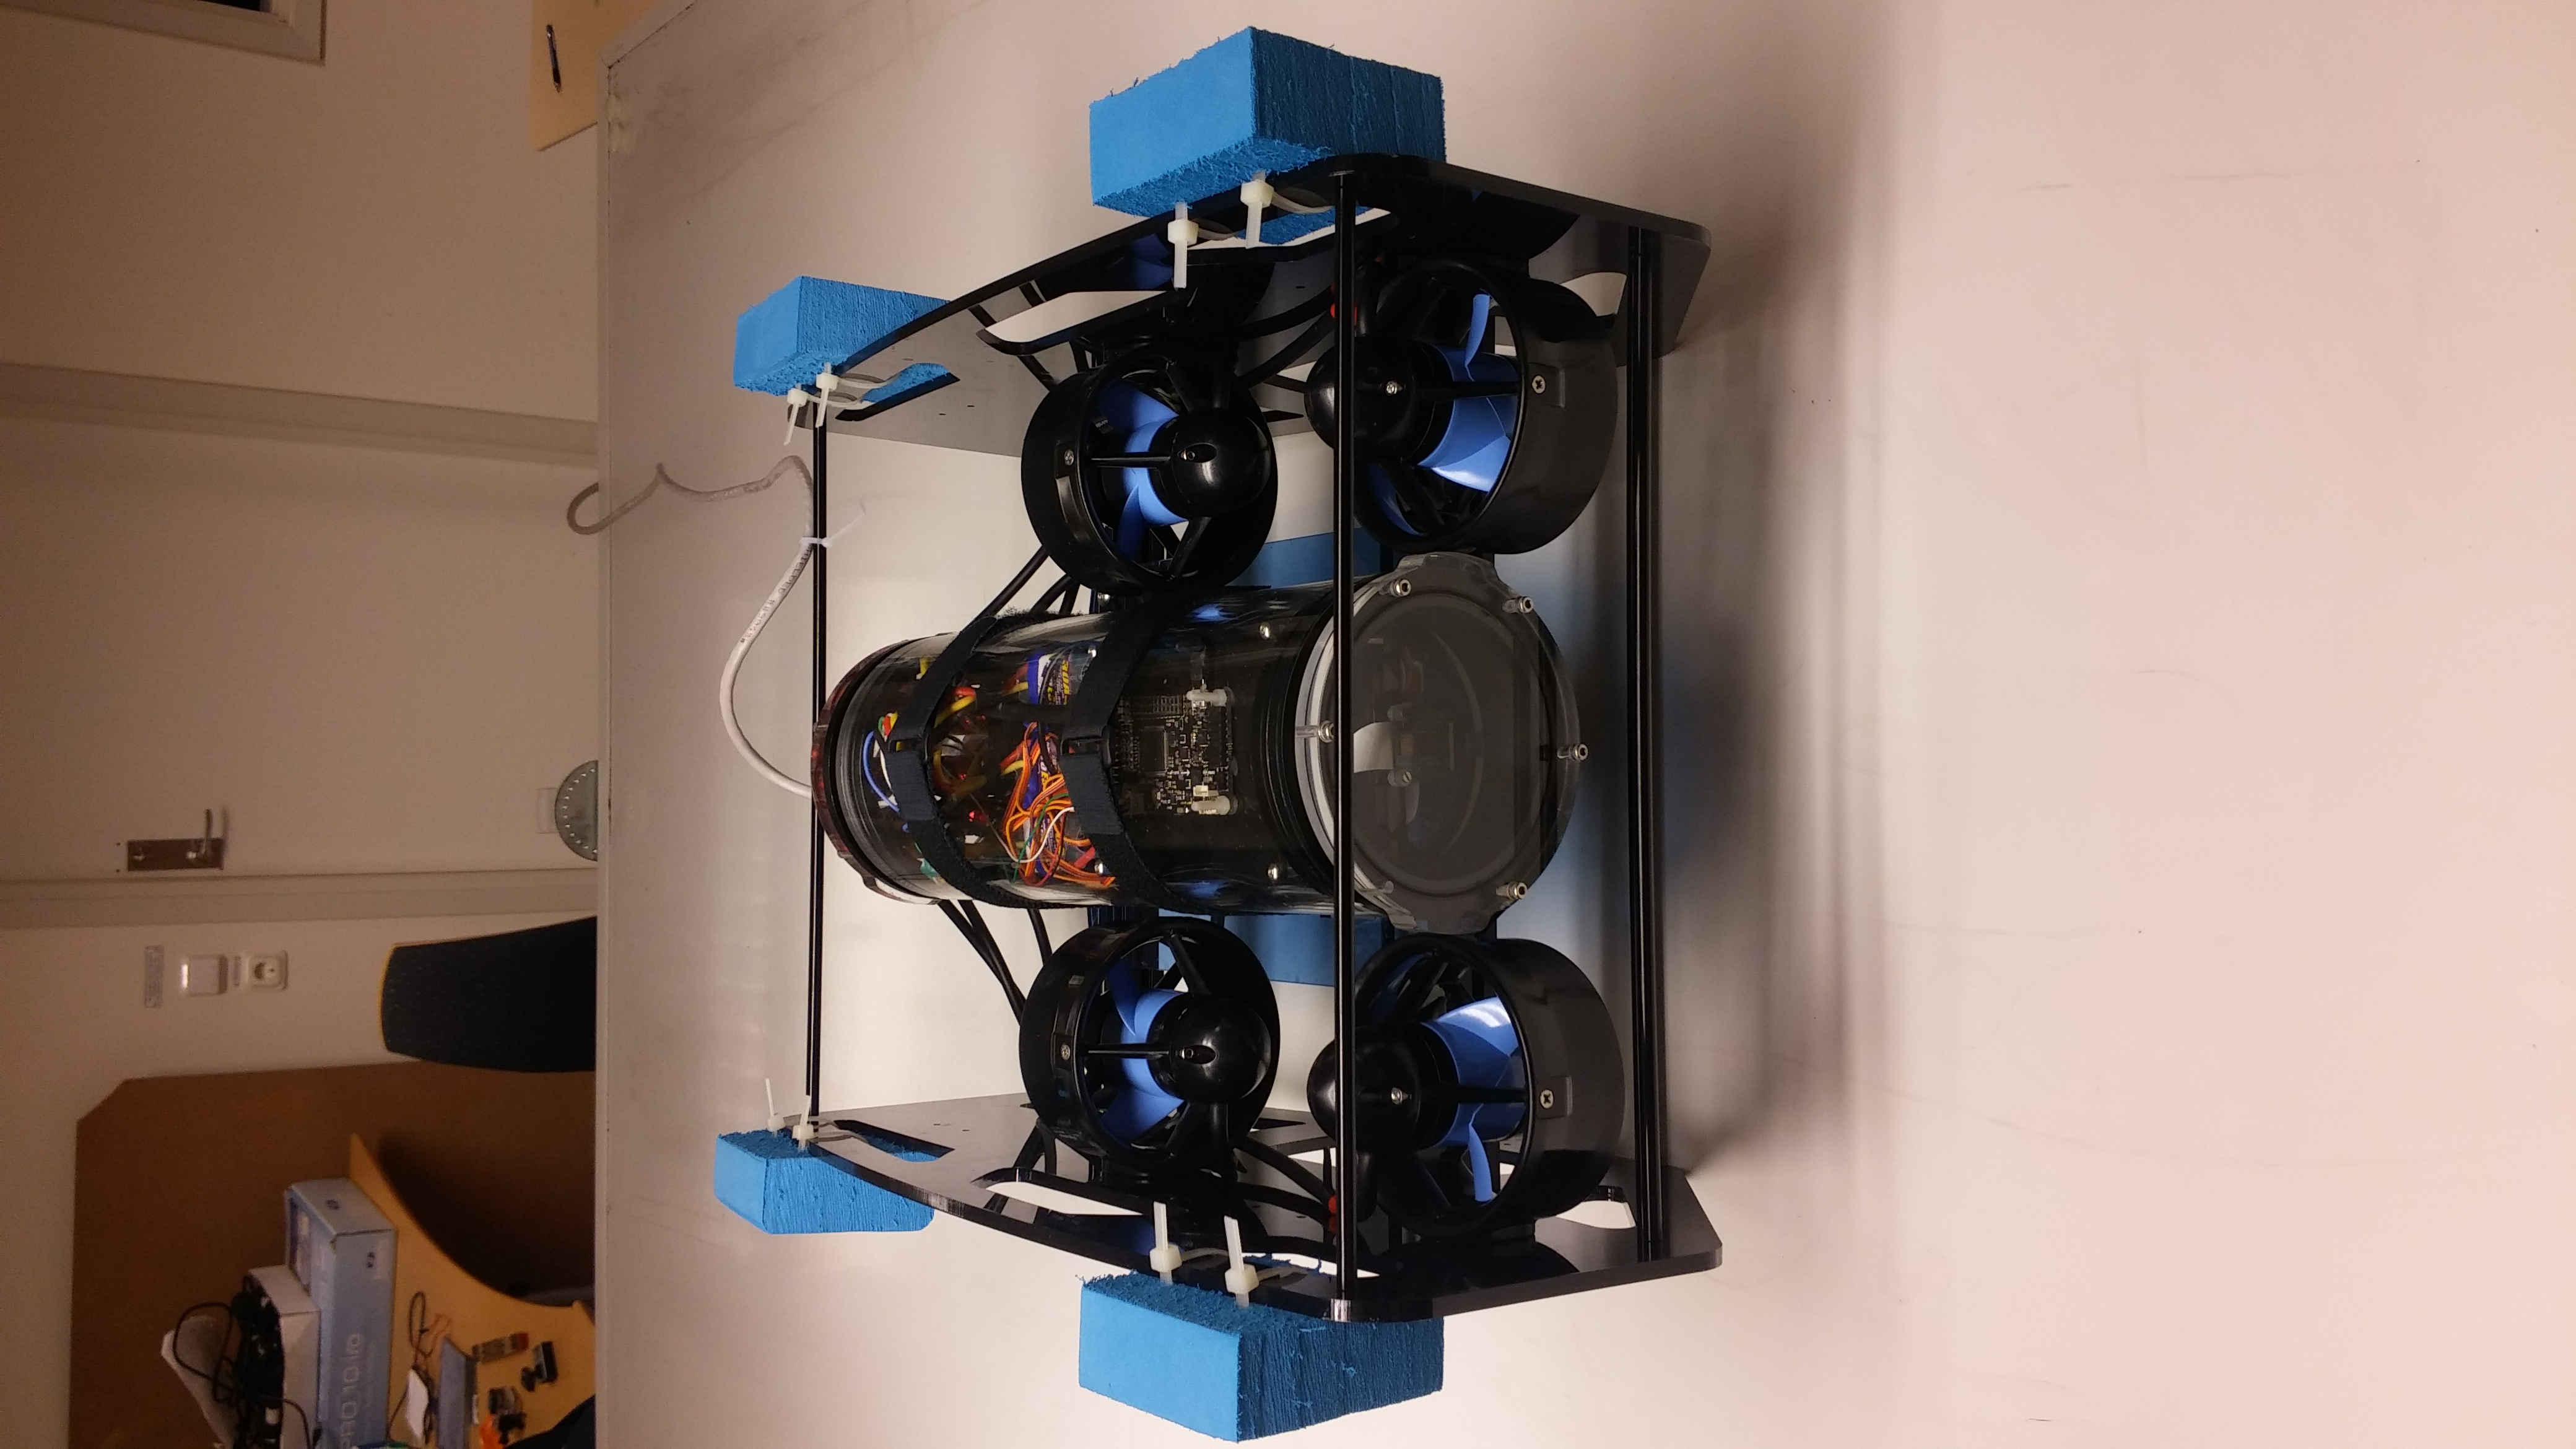
\includegraphics[trim={40cm 0cm 45cm 0cm},clip,angle=270,width=0.9\textwidth]{bluerov}
\caption{A frontal view of the BlueROV from Blue Robotics that was used in the thesis.
Note the four blue squares made of EVA foam mounted in the corners for extra buoyancy.}
\label{fig:rov}
\end{figure}

\section{ROV I/O}
The \abbrROV's \abbrIO consists of an HKPilot Mega 2.7 which is based on Ardupilot Mega. The HKPilot Mega 2.7 has the following on chip sensors
\begin{itemize}
    \item Magnetometer - HMC5883L.
    \item Barometer - MS5611-01BA.
    \item Inertial measurement unit (\abbrIMU) - MPU6000.
\end{itemize}
An external pressure sensor MS5837-30BA which was encased in a watertight case by Blue Robotics was connected to the HKPilot Mega 2.7 by \abbrIC.
The HKPilot Mega 2.7 also controls the six \abbrESC{}s. The \abbrESC{}s are 30A AfroESCs flashed with Blue Robotics linearising firmware. The HKPilot Mega 2.7 is connected to the onboard computer by \abbrUSB cable. The HKPilot Mega 2.7 runs a rosserial-arduino node which is a simpler \abbrROS node that communicates with a master node by serial communication. Scaling and calibration of the sensors are done automatically. However, the offset calibration of the magnetometer and accelerometer has to be performed manually by following the instructions that are produced in the workstation terminal window when the calibration script is run. The external pressure sensor uses the internal barometer to remove the atmospheric pressure offset. The atmospheric pressure offset is measured once, at the start up of the \abbrROV. \index{ROS@\abbrROS!abbreviation} \index{ESC@\abbrESC!abbreviation} 

\section{Power}
To power the \abbrROV a Turnigy 5000mAh 4S 25C Lipo Pack was used. This is a high discharge battery which ensures that all thrusters can be run at the same time without disruptive voltage drops.
To power the Raspberry Pi 2, a HobbyKing LiPo to \abbrUSB Charging Adapter was used. This adapter connects to the JST-XH connector on the LiPo battery and then outputs regular \abbrUSB voltages and currents. A \abbrUSB to micro-\abbrUSB adapter was used to route the power to the Raspberry Pi. 
The \abbrESC{}s are powered via the main lead of the LiPo battery. Lastly, the HKPilot Mega 2.7 is powered via \abbrUSB by the Raspberry Pi \textbf{and} by the \abbrESC{}s. 

\section{The Onboard Computer}
The onboard computer was a Raspberry Pi 2 Model B which can be seen in \Figureref{fig:raspberryandcamera}. A Raspicam was connected to the Raspberry Pi 2 and was used in conjunction with a \abbrROS node to create a video feed. 
The \abbrROS nodes running on the onboard computer can be seen in \Tableref{tab:raspnodes}.\index{ROS@\abbrROS!abbreviation} 
 \begin{table}[tbp]
  \centering
  \caption{\label{tab:raspnodes}%
    The different nodes that run on the onboard computer.}

  \begin{tabular}{l p{0.5\linewidth}}
    \toprule%
    \textbf{Node} & \textbf{Description} \\
    \otoprule%
    roscore             &  Node that handles the \abbrROS backend.\\

    raspicam\_node      &  Camera node for streaming video from the \abbrROV.\\
    
    controller          &  Node that can run different controllers.\\
    
    rosserial           &  Serial node for communication with the HKPilot Mega 2.7.\\
    \bottomrule%
  \end{tabular}
\end{table}

\begin{figure}
    \centering
    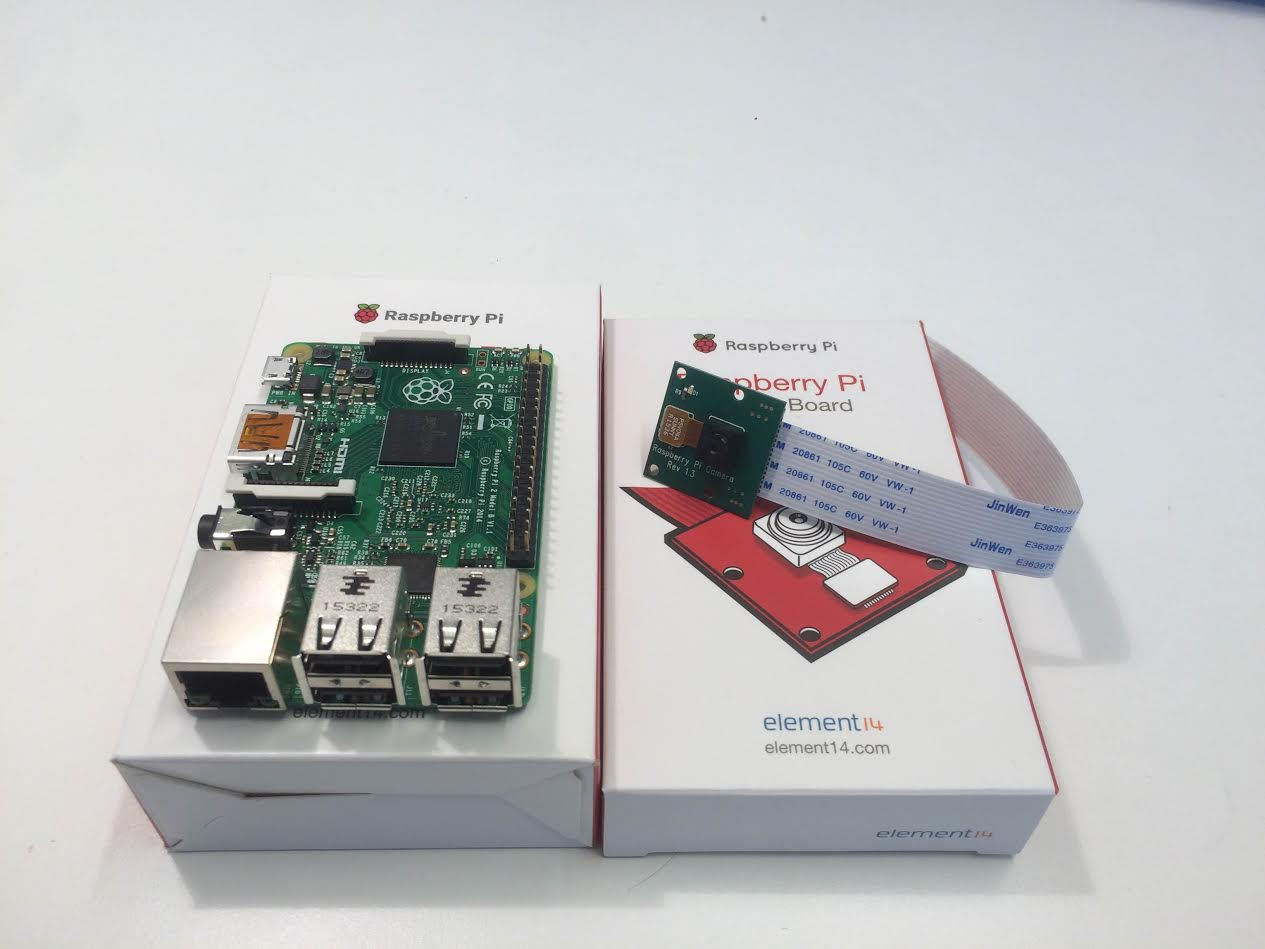
\includegraphics[trim={0 0 0 5cm},clip,width=0.9\textwidth]{raspberryandcamera}
    \caption{The Raspberry Pi 2 Model B, the onboard computer, is shown to the left and the raspicam is shown on the right.}
    \label{fig:raspberryandcamera}
\end{figure}

\begin{figure}
    \centering
    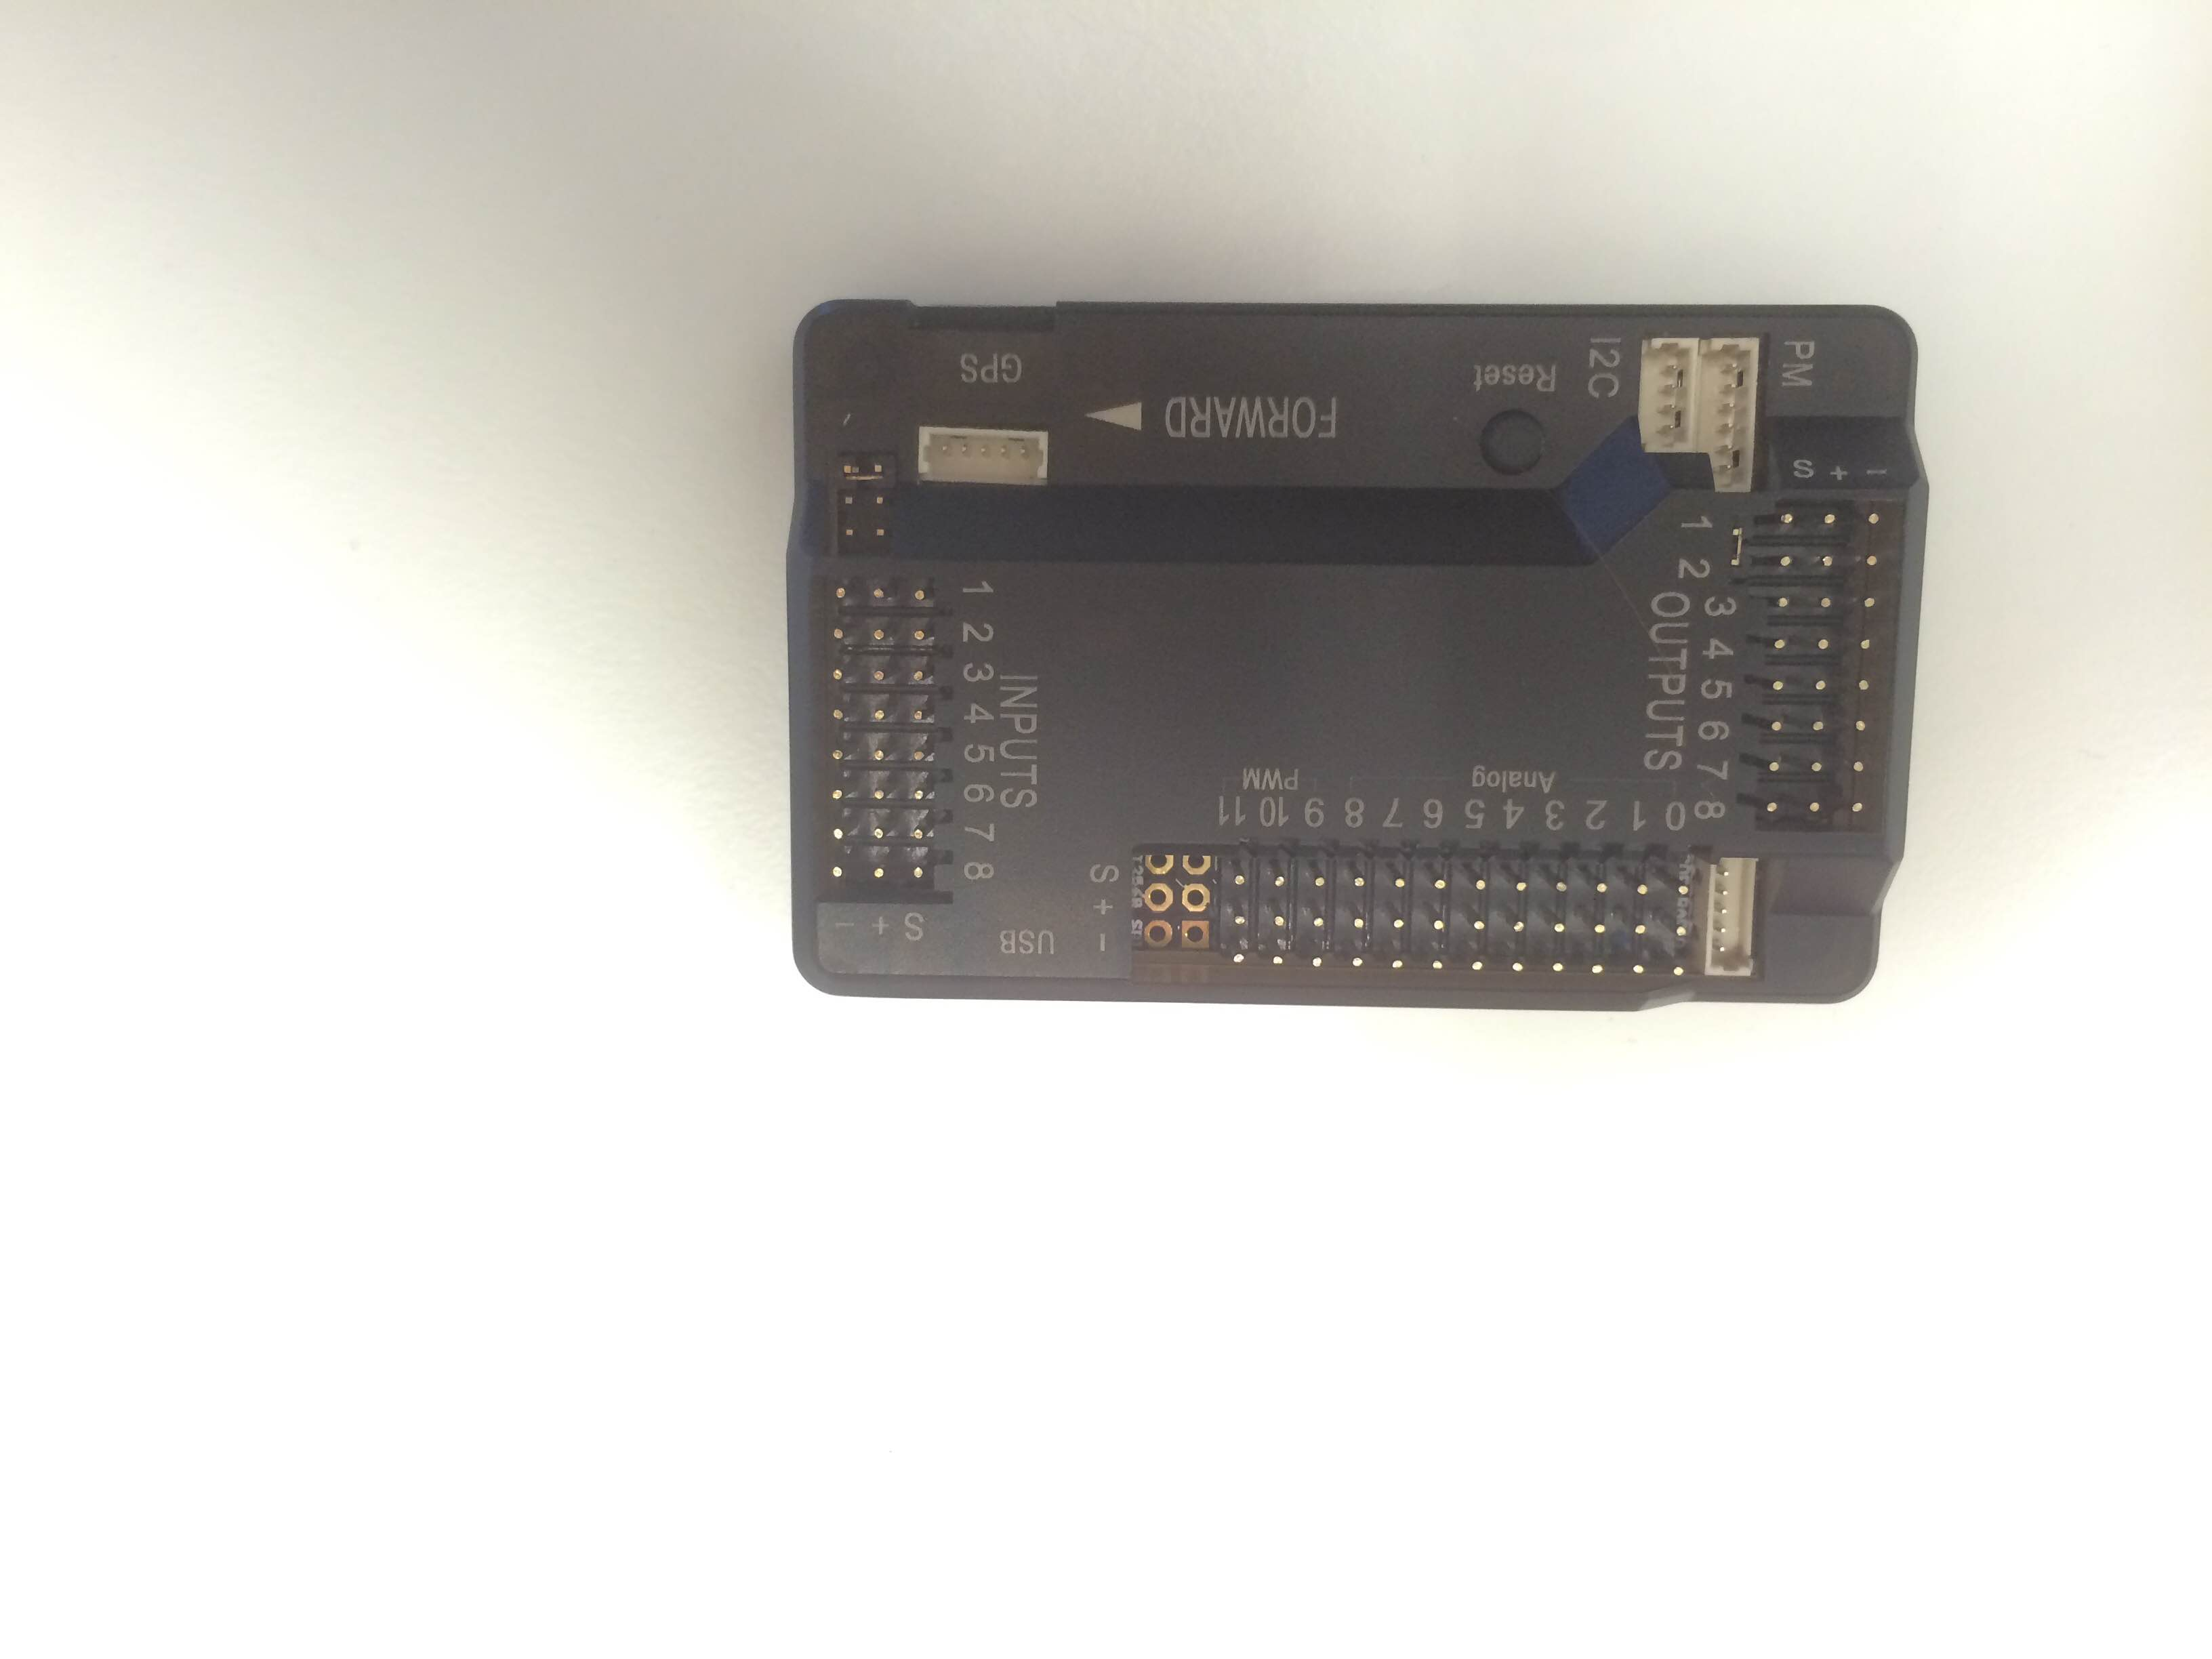
\includegraphics[trim={0 0 4cm 10cm},angle=180,origin=c,clip,width=0.9\textwidth]{apm}
    \caption{The HKPilot Mega 2.7 used for \abbrIO.}
    \label{fig:apm}
\end{figure}

\section{The Workstation}
The workstation used in the thesis is a Lenovo T430 with an Intel\textregistered i5-3210M processor and Intel\textregistered HD Graphics 4000. The workstation was connected via a Cat 6 tether to the Raspberry Pi 2. The different \abbrROS nodes that are run on the workstation can be seen in \Tableref{tab:workstationnodes}.\index{ROS@\abbrROS!abbreviation} 
\begin{table}[tbp]
  \centering
  \caption{\label{tab:workstationnodes}%
    The different nodes that run on the workstation.}

  \begin{tabular}{l p{0.5\linewidth}}
    \toprule%
    \textbf{Node} & \textbf{Description} \\
    \otoprule%
    heartbeat       & Node for checking the connection with the HKPilot Mega 2.7.\\

    teleop\_xbox    & Xbox node for handling inputs from the Xbox controller.\\

    joy             & A joystick node for interacting with the \abbrOS{}s \abbrUSB inputs.\\
        
    
    rqt             & A \abbrGUI for the \abbrROV.\\
    
    sensorfusion    & The sensor fusion node. \\
    \bottomrule%
  \end{tabular}
\end{table}
\chapter{Modelling the ROV} \label{cha:modelling}
This chapter will describe how our \abbrROV is modelled using \citet{fossen2011} 6 \abbrDOF model for \abbrROV's.

A underwater vehicle with 6 \abbrDOF, like our ROV, can be described by\index{Model of an underwater vehicle}
\begin{equation} \label{eq:model}
 \inertia \nuVectordot + \coriolis(\nuVector)\nuVector + \damping(\nuVector)\nuVector + \gravity(\etaVector) = \tauVector
\end{equation}
 
where
\begin{equation*}
  \listEta  
\end{equation*} are generalised positions and
\begin{equation*}
  \listNu 
\end{equation*}
are generalised velocities that are used to describe motion in 6 \abbrDOF. The matrices $\inertia$\index{Inertia matrix}, $\coriolis$\index{Coriolis matrix}, $\damping$\index{Damping matrix} and the vector $\gravity$\index{Restoring forces matrix} respectively describes how inertia, Coriolis forces, damping forces, gravity and buoyancy affect the \abbrROV. The vector $\tauVector$ describes the forces and torques produced by the \abbrROV's actuators and disturbances.
\todo[inline]{Write something about the different coordinate systems}


 
%%%%%%%%%%%%%%%%%%%%%%%%%%%%%%%%%%%%%%%%
In this chapter, the vector cross-product $\cross{\cdot}$ is defined as $\cross{a\boldsymbol{A}} \boldsymbol{B} = a\boldsymbol{A} \times \boldsymbol{B}$. The notation used for the parameters in this chapter and \Chapterref{cha:parameterEstimation} can be seen in \Tableref{tab:notationModelling}. The notation for forces, moments, linear and angular velocities, positions and Euler angles used in the model is summarised in \Tableref{tab:notationMarine}.

 \begin{table}[tbp]
  \centering
  \caption{\label{tab:notationModelling}%
    The notation and description of the parameters used in the \abbrROV model.}

  \begin{tabular}{l p{0.7\linewidth}}
    \toprule%
    \textbf{Notation} & \textbf{Description} \\
    \otoprule%
    $\bodyinertia{b}$ & Inertia matrix for rotation around \abbrCO.\\
    $\bodyinertia{g}$ & Inertia matrix for rotation around \abbrCG.\\
    $\Kp, \Mq,\Nr$    & Linear damping coefficients for rotation in water. \\
    $\Kpabsp, \Mqabsq,\Nrabsr$ & Quadratic damping coefficients for rotation in water. \\
    $\Kpdot, \Mqdot,\Nrdot$    & Increased inertia about $\xPosition, \yPosition, \zPosition$-axis due to rotation in water.\\
    $\Xu, \Yv, \Zw$ & Linear damping coefficients for translation in water.\\
    $\Xuabsu, \Yvabsv, \Zwabsw$ & Quadratic damping coefficients for translation in water.\\
    $\Xudot, \Yvdot, \Zwdot$   & Added mass in $\xPosition, \yPosition, \zPosition$-direction due to translation in water. \\
    $\distance{x}{i}, \distance{y}{i},\distance{z}{i}$. & Moment arms from \abbrCG to each thruster $i$. \\
    $m$ & The \abbrROV's mass \\
    $z_B$ & Distance between \abbrCB and \abbrCG along the $z$-axis. \\
    $V$ & Displaced volume. \\
    $\rho$ & Water density. \\
    $g$ & Gravity. \\
     $r^g_b$ & The distance between \abbrCO and \abbrCG. \\
    \bottomrule%
  \end{tabular}
\end{table}

 \begin{table}[tbp]
  \centering
  \caption{\label{tab:notationMarine}%
    The notation of \citet{sname} for marine vessels.}

  \begin{tabular}{l p{0.35\linewidth}  p{0.14\linewidth} p{0.14\linewidth} p{0.14\linewidth}}
    \toprule%
    \textbf{DOF} & \textbf{Description}  & \textbf{Forces and moments} & \textbf{Linear and angular velocities} & \textbf{Positions and Euler angles} \\
    \otoprule%
    1 & Motions in the x direction (surge).     & \xForce       & \xVelocity        & \xPosition \\
        
    2 & Motions in the y direction (sway).      & \yForce       & \yVelocity        & \yPosition \\
    
    3 & Motions in the z direction (heave).     & \zForce       & \zVelocity        & \zPosition \\
    
    4 & Rotation about the x axis (roll, heel). & \rollMoment   & \rollVelocity     & \rollAngle \\
    
    5 & Rotation about the y axis (pitch, trim).& \pitchMoment  & \pitchVelocity    & \pitchAngle \\
    
    6 & Rotation about the z axis (yaw).        & \yawMoment    & \yawVelocity      & \yawAngle \\
    \bottomrule%
  \end{tabular}
\end{table}

%%%%%%%%%%%%%%%%%%%%%%%%%%%%%%%%%%%%%%%%
\section{The body-fixed and global coordinate systems}
\label{sec:coordinates}\index{NED}\index{body-fixed coordinate system}\index{global coordinate system}
During modelling it is important to choose proper coordinate systems in which to describe the systems behaviour.
The \abbrROV model used in this thesis uses two separate coordinate systems.
The first system, the body-fixed coordinate system, is fixed to the \abbrROV and rotates with the \abbrROV. 
The body-fix coordinate system is a right-hand system, the $\xPosition$-axis is placed along the length of the \abbrROV pointing towards its bow. The $\yPosition$-axis points starboard, and the $\zPosition$-axis points downwards towards the vehicles keel. The coordinate system is assumed to be centred in the \abbrROV's \abbrCG. The body-fixed coordinate system makes it easier to describe sensor readings, since the sensors rotate with the \abbrROV. It is also easier to express the effect of each thruster in forces and moments described in the body-fixed coordinate system.

The global coordinate system is Earthfixed, with axes $\north$, $\east$ and $\down$. The $\north$ axis points in the direction of our calibrated North, the $\east$ axis points in the direction of calibrated East and the $\down$ axis points down towards the \abbrCG of the Earth.
This coordinate system is used to express buoyancy and gravitational forces on the \abbrROV, their effects are transformed to the local coordinate system by a rotation matrix. How the local and global coordinate systems relate to each other can be seen in \Figureref{fig:coordinate_frames}.

\newcommand*{\coordinateRadius}{0.05}
\newcommand*{\coordRot}{30}
\begin{figure}
    \centering
    \begin{tikzpicture}[scale=2]
        \pgfmathsetmacro\by{\coordinateRadius*sin(45)}
        \pgfmathsetmacro\bx{\coordinateRadius*cos(45)}
        \pgfmathsetmacro\ay{\coordinateRadius*sin(\coordRot)}
        \pgfmathsetmacro\ax{\coordinateRadius*cos(\coordRot)}
        \pgfmathsetmacro\coordYRot{sin(\coordRot)}
        \pgfmathsetmacro\coordXRot{cos(\coordRot)}
        
        \coordinate (O) at (0,0);
        \draw[thick,->] (O) ++(\coordinateRadius,0) -- ++(1,0) node[anchor=north east]{$\north$};
        \draw[thick,->] (O) ++(0,-\coordinateRadius)-- ++(0,-1) node[anchor=south east]{$\east$};
        \draw (O) circle (0.05) node[anchor=south,]{$\down$,\color{red}$\zPosition$};
        \draw (O) -- ++(\bx,\by) (O) -- ++(-\bx,-\by) (O) -- ++(-\bx,\by) (O)  -- ++(\bx,-\by);
        
        \draw[thick,red,->] (O) ++(\ax,-\ay) -- ++(\coordXRot,-\coordYRot) node[anchor=north west]{$\xPosition$};
        \draw[thick,red,->] (O) ++(-\ay,-\ax) -- ++(-\coordYRot,-\coordXRot) node[anchor=north east]{$\yPosition$};
        \draw[->] (O) ++(0.5,0) arc (0:-\coordRot:0.5) node[right]{\yawAngle};
        
        \def\coordDistance{1.5}
        
         \coordinate (O) at (\coordDistance,0);
         \draw[thick,->] (O) ++(\coordinateRadius,0) -- ++(1,0) node[anchor=north east]{$\north$};
         \draw[thick,->] (O) ++(0,-\coordinateRadius)-- ++(0,-1) node[anchor=south east]{$\down$};
         \draw (O) circle (0.05) node[anchor=south,]{$\east$,\color{red}$\yPosition$};
         \draw[fill=black] (O) circle (0.0125);
        
         \draw[thick,red,->] (O) ++(\ax,\ay) -- ++(\coordXRot,\coordYRot) node[anchor=south west]{$\xPosition$};
         \draw[thick,red,->] (O) ++(\ay,-\ax) -- ++(\coordYRot,-\coordXRot) node[anchor=north east]{$\zPosition$};
         \draw[->] (O) ++(0.5,0) arc (0:\coordRot:0.5) node[right]{\pitchAngle};
         
          
        \pgfmathsetmacro\coordDistanceZ{2*\coordDistance+1}
        
         \coordinate (O) at (\coordDistanceZ,0);
         \draw[thick,->] (O) ++(-\coordinateRadius,0) -- ++(-1,0) node[anchor=north west]{$\east$};
         \draw[thick,->] (O) ++(0,-\coordinateRadius) -- ++(0,-1) node[anchor=south east]{$\down$};
         \draw (O) circle (0.05) node[anchor=south,]{$\north$,\color{red}$\xPosition$};
         \draw[fill=black] (O) circle (0.0125);
        
        \draw[thick,red,->] (O) ++(\ay,-\ax) -- ++(\coordYRot,-\coordXRot) node[anchor=north west]{$\zPosition$};
        \draw[thick,red,->] (O) ++(-\ax,-\ay) -- ++(-\coordXRot,-\coordYRot) node[anchor=south east]{$\yPosition$};
        \draw[->] (O) ++(-0.5,0) arc (180:180+\coordRot:0.5) node[left]{\rollAngle};
    
    \end{tikzpicture}
    \caption{The local and global coordinate systems relate to each other by the rotations \yawAngle, \pitchAngle and \rollAngle. The rotations are defined from the global coordinate system (black) to the body-fixed coordinate system (red).} 
    \label{fig:coordinate_frames}
\end{figure}

\todo[inline]{Write about kinetics}
\missingfigure{Picture of the rov with the coordinate system.}

%%%%%%%%%%%%%%%%%%%%%%%%%%%%%%%%%%%%%%%%
\section{Inertia}
The inertia matrix $\inertia$ describes the resistance of moving and rotating the \abbrROV in its 6 \abbrDOF. It also describes the added mass that comes from rotating and translating a body in a liquid media. The inertia matrix is defined as
\begin{equation}
    \inertia = \inertia_{RB}+\inertia_{A}
\end{equation}
where $\inertia_{RB}$ is the inertia Matrix for a rigid-body and $\inertia_{A}$ is the added mass \citep{fossen2011}.\index{Added mass} \index{Inertia}

The inertia matrix, $\inertia_{RB}$, for a rigid-body is defined as
\begin{equation}
\label{eq:inertia}
    \inertia_{RB} = 
    \begin{pmatrix}
    m\eye{3}       & -m\cross{r^b_g} \\
    m\cross{r^b_g} & \bodyinertia{b}
    \end{pmatrix}
\end{equation}
where $r^b_g$ is the distance between the \abbrROV's \abbrCO and \abbrCG \citep[p.52]{fossen2011}.
It has been assumed that the \abbrROV's \abbrCO and \abbrCG coincide, thus simplifying \eqref{eq:inertia} to
\begin{equation}
   \inertia_{RB} = 
    \begin{pmatrix}
        m\eye{3} & \zero{3} \\
        \zero{3} & \bodyinertia{g}
    \end{pmatrix}
\end{equation} 
The added mass of the water, $\inertia_A$, acting upon the \abbrROV is defined as
\begin{equation}
\inertia_A =
-\begin{pmatrix}
    \Xudot & 0 & 0 & 0 & 0 & 0 \\
    0 & \Yvdot & 0 & 0 & 0 & 0 \\
    0 & 0 & \Zwdot & 0 & 0 & 0 \\
    0 & 0 & 0 & \Kpdot& 0 & 0 \\
    0 & 0 & 0 & 0 & \Mqdot & 0 \\
    0 & 0 & 0 & 0 & 0 & \Nrdot \\
    \end{pmatrix}
\end{equation}
under the assumption that the \abbrROV moves at low speeds relative to the water \citep[p.121]{fossen2011}.
%%%%%%%%%%%%%%%%%%%%%%%%%%%%%%%%%%%%%%%%
\section{Coriolis forces}
Since the \abbrROV travels in a rotating reference frame, the Earth, the \abbrROV is subjected to inertial forces called Coriolis forces. The Coriolis forces acting on the \abbrROV are described in a similar manner to the inertia matrix, $\inertia$, with
\begin{equation}
    \coriolis(\nuVector) = \coriolis_{RB}(\nuVector) + \coriolis_A(\nuVector)
\end{equation}\citep[p.110]{fossen2011}. $\coriolis_{RB}(\nuVector)$ describes the Coriolis and centripetal forces caused by the rigid body's mass, while $\coriolis_A(\nuVector)$ describe the same effects but caused by the added inertia and mass.\index{Added mass}\index{Coriolis}

The rigid-body Coriolis vector is given as
\begin{equation}
\begin{split}
    \coriolis_{RB}(\nuVector)\nuVector &= 
    \begin{pmatrix}
        m\cross{\nuVectorAng}              & -m\cross{\nuVectorAng}\cross{r_g^b}  \\
        m\cross{r_g^b}\cross{\nuVectorAng} & -\cross{\bodyinertia{b}\nuVectorAng} \\
    \end{pmatrix}
    \nuVector = 
    \begin{pmatrix}
    m (q w-r v) \\
    m (r u-p w) \\
    m (p v-q u) \\
    q r(\bodyinertiaconstant{y}-\bodyinertiaconstant{z}) \\
    r p(\bodyinertiaconstant{z}-\bodyinertiaconstant{x}) \\
    q p(\bodyinertiaconstant{x}-\bodyinertiaconstant{y}) \\
    \end{pmatrix}
\end{split}
\end{equation}
where it has been assumed that the \abbrROV is symmetric about the $xyz$-plane to eliminate cross-terms in $\coriolis(\nuVector)$\citep[p.55]{fossen2011}.
The Coriolis and centripetal effects from the added mass are described as
\begin{equation}
\begin{split}
    \coriolis_A(\nuVector) \nuVector &= 
    \begin{pmatrix}
    0 & 0 & 0 & 0 & -\Zwdot w & \Yvdot v \\
    0 & 0 & 0 & \Zwdot w & 0 & -\Xudot u \\
    0 & 0 & 0 & -\Yvdot v & \Xudot u & 0 \\
    0 & -\Zwdot w & \Yvdot v & 0 & -\Nrdot r & \Mqdot q \\
    \Zwdot w & 0 & -\Xudot u & \Nrdot r & 0 & -\Kpdot p \\
    -\Yvdot v & \Xudot u & 0 & - \Mqdot q & \Kpdot p & 0 \\
    \end{pmatrix}
    \nuVector = \\ 
    &= \begin{pmatrix}
        \Yvdot v r - \Zwdot w q\\
        \Zwdot w p - \Xudot u r\\
        \Xudot u q - \Yvdot v p \\
        (\Yvdot - \Zwdot) v w + (\Mqdot - \Nrdot) q r\\
        (\Zwdot - \Xudot) u w + (\Nrdot - \Kpdot) p r\\
        (\Xudot - \Yvdot) u v + (\Kpdot - \Mqdot) p q \\
    \end{pmatrix}
\end{split}
\end{equation} Under the assumption that the \abbrROV is moving slowly and has three planes of symmetry \citep[p.121]{fossen2011}. 
%%%%%%%%%%%%%%%%%%%%%%%%%%%%%%%%%%%%%%%%
\section{Viscous damping}
There are four main sources of hydrodynamic damping acting upon a submersed vehicle \citep[p.122]{fossen2011}.
Potential damping, skin friction, wave drift damping and damping from vortex shedding. The effects of these four sources on a 6 \abbrDOF vehicle can be described by two 6-by-6 matrices.\index{Viscous damping}
The matrix $\damping$ contains the linear damping terms, while the matrix $\damping_{n}(\nuVector)$ contains the quadratic, or non-linear, damping terms \citep{fossen2011}. The sum of these two matrices form the Viscous damping matrix $\damping(\nuVector)$ which in turn can be simplified to
\begin{equation}
\begin{split}
    \damping(\nuVector) &= \damping + \damping_{n}(\nuVector) = \\
    -& \scalemath{0.7}{\begin{pmatrix}
        \Xu+\Xuabsu\abs{u} & 0 & 0 & 0 & 0 & 0 \\
        0 & \Yv+\Yvabsv\abs{v} & 0 & 0 & 0 & 0 \\
        0 & 0 & \Zw+\Zwabsw\abs{w} & 0 & 0 & 0 \\
        0 & 0 & 0 & \Kp+\Kpabsp\abs{p} & 0 & 0 \\
        0 & 0 & 0 & 0 & \Mq+\Mqabsq\abs{q} & 0 \\
        0 & 0 & 0 & 0 & 0 & \Nr+\Nrabsr\abs{r} \\
    \end{pmatrix}}
\end{split}
\end{equation}
If the \abbrROV is symmetric about the $xz$-plane and the damping is assumed to be decoupled, $\damping(\nuVector)$ is a diagonal matrix \citep[p.129-130]{fossen2011}. The following vector is obtained when $\damping(\nuVector)$ is multiplied with $\nuVector$
\begin{equation}
    \damping(\nuVector) \nuVector =
     -\begin{pmatrix}
    (\Xu + \Xuabsu \abs{u}) u\\
    (\Yv + \Yvabsv \abs{v}) v\\
    (\Zw + \Zwabsw \abs{w}) w\\
    (\Kp + \Kpabsp \abs{p}) p\\
    (\Mq + \Mqabsq \abs{q}) q\\
    (\Nr + \Nrabsr \abs{r}) r\\
    \end{pmatrix}    
\end{equation}.



%%%%%%%%%%%%%%%%%%%%%%%%%%%%%%%%%%%%%%%%
\section{Restoring forces}\index{Restoring forces}\index{buoyancy}
Since the \abbrROV is submerged it will experience forces and moments caused by the Earths gravitational pull and the buoyancy force, in hydrostatic terms these are called restoring forces and act as spring forces on the \abbrROV \citep{fossen2011}. The restoring forces and moments are calculated using four main parameters; the mass of the vehicle, $m$, its buoyancy $B$ and lastly the coordinates for the \abbrROV's \abbrCG and center of buoyancy (\abbrCB) \citep{fossen2011}.
The restoring forces matrix, $\gravity(\etaVector)$, according to \citet[p.60]{fossen2011} defined as
\begin{equation}
    g(\etaVector) =
    \begin{pmatrix}
        (W - B) \sin \pitchAngle\\
    -(W - B) \cos \pitchAngle \sin \rollAngle\\
    -(W - B) \cos \pitchAngle \sin \rollAngle\\
    -z_B B \cos \pitchAngle \sin \rollAngle\\
    -z_B B \sin \pitchAngle\\
    0\\
    \end{pmatrix}
\end{equation}
describes how the forces and moments caused by the buoyancy force and gravitational pull of the Earth act on a 6 \abbrDOF model. Here $B$ is given by $B = \rho g V$ and $W = m g$. $m$ is the \abbrROV's mass, $g$ the gravitational constant, $\rho$ the density of water and $V$ the volume of displaced water. In other words the magnitude of the buoyancy forces is equal to the weight of the displaced water. For a fully submerged vehicle, $V$ will naturally be equal the volume of the vehicle.
In these calculations it is assumed that the \abbrCG coincides with the \abbrCO and that the \abbrCB lies at coordinate $[0, 0, z_B]$, directly above or below the \abbrCO. Note that the positions of the three centers are described using the coordinate system described in \Sectionref{sec:coordinates}, a roll and pitch stable \abbrROV should thus have a $z_B < 0$.

%%%%%%%%%%%%%%%%%%%%%%%%%%%%%%%%%%%%%%%%
\section{Thrust Matrix}
\missingfigure{Picture of the moments and forces including the name of the thrusters.}
The \abbrROV's actuators can be modelled as
\begin{equation}
    \tauVector = \thrusterGeometry \boldsymbol{\thrusterfun{}} 
\end{equation}
where $\thrusterGeometry$\index{thruster geometry} is a matrix describing the geometry of the actuators, see \Figureref{fig:thrusterlocation} \citep[p.401]{fossen2011}.
\begin{equation}
\begin{split}
    \tauVector = \thrusterGeometry \boldsymbol{\thrusterfun{}} 
    &=
    \begin{pmatrix}
    0& 0& 1& 1& 0& 0\\
    0& 0& 0&  0& 0& -1\\
    -1& -1& 0& 0& -1& 0\\
    \distance{y}{1} & -\distance{y}{2} & 0 &  0 &  0 & \distance{z}{6} \\
    \distance{x}{1} & \distance{x}{2} & 0 & 0 & -\distance{x}{5} & 0 \\
    0 & 0 & \distance{y}{3} & -\distance{y}{4} & 0 & 0 \\
    \end{pmatrix}
    \begin{pmatrix}
    \thrusterfun{1} \\
    \thrusterfun{2} \\
    \thrusterfun{3} \\
    \thrusterfun{4} \\
    \thrusterfun{5} \\
    \thrusterfun{6} \\
    \end{pmatrix}
    = \\
    &=\begin{pmatrix}
     \thrusterfun{3} + \thrusterfun{5} g \\
     -\thrusterfun{6} \\
     -\thrusterfun{1} - \thrusterfun{2} - \thrusterfun{4} \\
    \thrusterfun{2} \distance{y}{2} - \thrusterfun{1} \distance{y}{1} + \thrusterfun{6} \distance{z}{6} \\
    \thrusterfun{2} \distance{x}{2} - \thrusterfun{1} \distance{x}{1} - \thrusterfun{4} \distance{x}{4} \\
    \thrusterfun{3} \distance{y}{3} - \thrusterfun{5} \distance{y}{5} \\
    \end{pmatrix}
\end{split}
\end{equation}
where \distance{x}{1}, \distance{x}{2}, \distance{y}{1}, \distance{y}{2}, \distance{y}{3}, \distance{y}{4} and \distance{z}{6} are the offsets in the $x$, $y$ or $z$ direction of the $n$:th thruster and $\thrusterfun{i}$ is a lookup table from control signal to thrust in Newtons. See \appref{app:thrustmapping} for details regarding the lookup table.
\todo[inline]{Write \appref{app:thrustmapping}.}
%%%%%%%%%%%%%%%%%%%%%%%%%%%%%%%%%%%%%%%%
\section{Equations in Component Form}
If the matrices and vectors in \eqref{eq:model} are substituted with the matrices and vectors previously defined in this chapter and \eqref{eq:model} then solved for $\nuVectordot$ the following equations can be derived 
\begin{multline} \label{eq:u_dot}
\dot{u} = \frac{\thrusterfun{3} + \thrusterfun{4}}{m -\Xudot} + \frac{u (\Xu + \Xuabsu \abs{u})}{m -\Xudot} + \frac{\sin(\theta)(B - W)}{m -\Xudot} +\\
\frac{m(r v - q w )}{m -\Xudot} + \frac{-\Yvdot r v}{m -\Xudot} + \frac{\Zwdot q w}{m -\Xudot},
\end{multline}
\begin{multline} \label{eq:v_dot}
\dot{v} = \frac{-\thrusterfun{6}}{m - \Yvdot} + \frac{v (\Yv + \Yvabsv \abs{v})}{m - \Yvdot} + \frac{-\cos{\theta} \sin{\phi}(B - W)}{m - \Yvdot} +\\ \frac{m(p w - r u)}{m - \Yvdot} + \frac{\Xudot r u}{m - \Yvdot} + \frac{-\Zwdot p w}{m - \Yvdot},
\end{multline}
\begin{multline} \label{eq:w_dot}
\dot{w} = \frac{-\thrusterfun{1} - \thrusterfun{2} - \thrusterfun{5}}{m - \Zwdot} + \frac{w (\Zw + \Zwabsw \abs{w})}{m - \Zwdot} + \frac{-\cos{\phi}\cos{\theta}(B - W)}{m - \Zwdot} +\\
\frac{m (q u - p v)}{m - \Zwdot} + \frac{-\Xudot q u}{m - \Zwdot} + \frac{\Yvdot p v}{m - \Zwdot},
\end{multline}
\begin{multline} \label{eq:p_dot}
\dot{p} = \frac{\thrusterfun{1} \distance{y}{1} - \thrusterfun{2} \distance{y}{2} + \thrusterfun{6} \distance{z}{6}}{\Ix - \Kpdot} + \frac{p (\Kp + \Kpabsp \abs{p})}{\Ix - \Kpdot} + \frac{-\Mqdot q r}{\Ix - \Kpdot} + \frac{\Nrdot q r}{\Ix - \Kpdot} +\\
\frac{q r (\Iy - \Iz)}{\Ix - \Kpdot} + \frac{- \Yvdot v w}{\Ix - \Kpdot} + \frac{\Zwdot v w}{\Ix - \Kpdot} + \frac{B \cos{\theta} \sin{\phi} z_B}{\Ix - \Kpdot},
\end{multline}
\begin{multline} \label{eq:q_dot}
\dot{q} =\frac{\thrusterfun{1} \distance{x}{1} + \thrusterfun{2} \distance{x}{2} - \thrusterfun{5} \distance{x}{5}}{\Iy - \Mqdot} + \frac{q (\Mq + \Mqabsq \abs{q})}{\Iy - \Mqdot} + \frac{\Kpdot p r}{\Iy - \Mqdot} + \frac{-\Nrdot p r}{\Iy - \Mqdot} +\\
\frac{p r (\Iz - \Ix)}{\Iy - \Mqdot} + \frac{-\Zwdot u w}{\Iy - \Mqdot} + \frac{\Xudot u w}{\Iy - \Mqdot} + \frac{B \sin{\theta} z_B}{\Iy - \Mqdot} 
\end{multline} and 
\begin{multline} \label{eq:r_dot}
\dot{r} = \frac{\thrusterfun{3} \distance{y}{3} - \thrusterfun{4} \distance{y}{4}}{\Iz - \Nrdot} + \frac{r (\Nr + \Nrabsr \abs{r})}{\Iz - \Nrdot} + \frac{-\Kpdot p q}{\Iz - \Nrdot} + \frac{\Mqdot p q}{\Iz - \Nrdot} +\\
\frac{p q (\Ix - \Iy)}{\Iz - \Nrdot} + \frac{- \Xudot u v}{\Iz - \Nrdot} + \frac{\Yvdot u v}{\Iz - \Nrdot}
\end{multline} 
\chapter{Sensor fusion}
In order to properly estimate its attitude in the global coordinate system the \abbrROV needs sensor to measure inputs from its environment.
Unfortunately signals from sensors do not necessarily give direct information about attitude and are to some extent noisy. Smart algorithms and filters can nevertheless be used to extract and combine the information from the different sensors into a high certainty attitude estimate. The combination, or fusion, of several sensor sources into a estimate goes under the name sensor fusion. One filter that can accomplish the task of fusing different measurements and estimating states in a non-linear dynamic system is the extended Kalman filter (\abbrEKF). 
\section{Filter notation}
To be able to understand how a filter like the extended Kalman filter works, it is important to understand the notation. In table \ref{tab:notationKalman} the notation used in this chapter is listed.
 \begin{table}[htbp]
  \centering
  \caption{\label{tab:notationKalman}%
    The notation used for describing the extended Kalman filter.}
    \begin{tabular}{l p{0.7\linewidth}}
    \toprule%
    \textbf{Notation} & \textbf{Description} \\
    \otoprule%
    $x$ & State vector.\\
    $\hat{x}$ & State vector estimate.\\
    $y$    & Measurement vector.\\
    $u$ & Control signal.\\
    $v,e$ & Noise.\\
    $_k$ & At time k.\\
    $_{k|m}$ & At time $k$ given information up to time $m$.\\
    $f_x$ & Jacobian of $f$ with respect to states.\\
    $f_v$ & Jacobian of $f$ with respects to noise.\\
    $E(x)$ & The expected value of x.\\
    $Cov(x)$ & The covariance of x.\\
    \bottomrule%
 \end{tabular}
\end{table}

\section{The extended Kalman filter}
According to \citet{sensorfusion} the Kalman filter (\abbrKF) is a linear state space observer, meaning that it estimates states, both measurable and unmeasurable, in a linear system. It utilises a motion model, a model of the systems dynamics, in conjunction with measurements to provide the best possible estimate of the model's states. It's also stated in \citet{sensorfusion} that the Kalman filter finds the best possible linear filter for the given input $y_{k}$. The extended Kalman filter can, unlike the regular Kalman filter, handle non-linear motion models and measurement equations. It accomplishes this by using Taylor expansions of the non-linear system and measurement equations to approximate a linear system. If a \abbrEKF can provide satisfactory results depends on the rest terms from the Taylor expansion and it is therefore dependent on the degree of non-linearity of the system and measurement equations\citep{sensorfusion}. As rule of thumb the rest term will be small enough if the system model is close to linear and if measurements are of good quality, meaning that the signal to noise ration is high\citep{sensorfusion}. 

The \abbrEKF algorithm is comprised of two key steps called updates.
The time update uses the current states estimates and the user specified motion model to predict the values of the states the next time instant. The second update is called the measurement update and it uses sampled sensor data in conjunction with the user specified measurement equations to strengthen the state estimates. \todo{Reference needed!}
The order in which to run these updates is dependent on design and on sample time of the sensors used. If the measurements are independent a measurement update can be done at the arrival of each measurement without the need of a time update in between\citep[p.170]{sensorfusion}.

The complete extended Kalman filter algorithm can be viewed in \ref{alg:EKF}.
\begin{algorithm}
\label{alg:EKF}
\caption{The extended Kalman filter algorithm.}
  The extended Kalman filter applied on a system
    \begin{align*}
    x_{k+1} &= f(x_{k},u_{k},v_{k})\\
    y_{k} &= h(x_{k},u_{k},e_{k})
    \end{align*} is given by the following algorithm:\\
    \textbf{Initialisation:}
    \begin{align*}
    \hat{x}_{1|0} &= E(x_{0})\\
    P_{1|0} &= Cov(x_{0})\\
    \end{align*}
     
    \textbf{Measurement update:}
    \begin{align*}
    S_{k} &= h_{x}(\hat{x}_{k|k-1},u_ {k}) P_{k|k-1} h_{x}(\hat{x}_{k|k-1},u_ {k})^{T} + R_{k}\\
    K_{k} &= P_{k|k-1} h_{x}(\hat{x}_{k|k-1},u_ {k})^{T} S_{k}^{-1}\\
    \hat{x}_{k|k} &= \hat{x}_{k|k-1} + K_{k} (y_{k} - h(\hat{x}_{k|k-1},u_ {k}))\\
    P_{k|k} &= P_{k|k-1} - P_{k|k-1} h_{x}(\hat{x}_{k|k-1},u_ {k})^{T} S_{k}^{-1} h_{x}(\hat{x}_{k|k-1},u_ {k}) P_{k|k-1}\\
    \end{align*}
    
   \textbf{Time update:}
    \begin{align*}
    \hat{x}_{k+1|k} &= f(\hat{x}_{k|k},u_ {k})\\
    P_{k+1|k} &= f_{x}(\hat{x}_{k|k},u_ {k})P_{k|k} f_{x}(\hat{x}_{k|k},u_ {k})^{T} + f_{v}(\hat{x}_{k|k},u_ {k}) Q_{k} f_{v}(\hat{x}_{k|k},u_ {k})^{T}
    \end{align*}    
\end{algorithm}

\section{Motion model}
A Kalman filter uses knowledge of the system dynamics to strengthen the estimates of the models states. It is therefore very important to choose a model the sufficiently describes the systems dynamics. The better the model the better performance of the filter. In this thesis a simple motion model with quaternions $Q$, angular velocities $\omega$, gyro biases $b_{\omega}$ and depth $d$ as states was used. The model is based on the work of \todo{Hitta avhandlingen som Jonas prata om} and when is when discretised 
\begin{equation}
\begin{split}
\begin{pmatrix}
Q_{k+1}\\
\omega_{k+1}\\
b_{k+1}\\
d_{k+1}
\end{pmatrix}&=
\left(
\begin{array}{c|c|c|c}
I_{4\times4} + \frac{T}{2}S(\omega_{k})& \frac{T^2}{2} \bar{S}(Q_{k}) & 0_{4\times3} & 0_{4\times1} \\
\hline
0_{3\times4} & I_{3\times3} & 0_{3\times3} & 0_{3\times1}\\
\hline
0_{3\times4} & 0_{3\times3} & I_{3\times3} & 0_{3\times1}\\
\hline
0_{1\times4} & 0_{1\times3} & 0_{1\times3} & I_{1\times1}\\
\end{array}
\right)
\begin{pmatrix}
Q_{k}\\
\omega_{k}\\
b_{k}\\
d_{k}
\end{pmatrix}
\\ &+\left(\begin{array}{c|c|c}
\frac{T^3}{4}\bar{S}(Q_{k}) & 0_{3\times3} & 0_{3\times1}\\
\hline
T I_{3\times3}& 0_{3\times3} & 0_{3\times1}\\
\hline
0_{3\times3} & T I_{3\times3} & 0_{3\times1}\\
\hline
0_{1\times3} & 0_{1\times3} & T I_{1\times1}\\
\end{array}
\right)
\begin{pmatrix}
v_{\omega}\\
v_{bias}\\
v_{d}
\end{pmatrix}
\end{split}
\end{equation}
where
\begin{equation}
S(\omega_{k}) = \begin{pmatrix}
    0 & -p_{k} & -q_{k} & -r_{k} \\
     p_{k} & 0 & r_{k} & -q_{k} \\
     q_{k} & -r_{k} & 0 & p_{k} \\
     r_{k} & q_{k} & -p_{k} &0
\end{pmatrix}
\end{equation},
\begin{equation}
\omega_{k} = \begin{pmatrix}
p_{k}\\
q_{k}\\
r_{k}
\end{pmatrix}
\end{equation}
and
\begin{equation}
\bar{S}(Q_{k}) = \begin{pmatrix}
    -Q_{1,k} & -Q_{2,k} & -Q_{3,k}\\
    Q_{0,k} & -Q_{3,k} &  Q_{2,k}\\
    Q_{3,k} &  Q_{0,k} & -Q_{1,k}\\
    -Q_{2,k} & Q_{1,k} &  Q_{0,k}
\end{pmatrix}
\end{equation}. Here $p$, $q$ and $r$ represent roll-, pitch- and yaw-rate. $Q_0$ \rightarrow $Q_3$ are quaternions which are used to represent the attitude of the \abbROV.

%Since $Cov(v_{k})$, $Cov(e_{k})$ and $Cov(x_{0})$ often can be hard to properly estimate, the matrices $Q_{k}$, $R_{k}$ and $P_{1|0}$ can be seen as design variables denoting certainty in the model, sensors and initial state.
%It is important to note that several time updates or measurement updates can be made in a row. One may for example run a time update at a given rate, while measurements are received sporadically.\citep[p.170]{sensorfusion}

\subsection{Gyro measurement equation}
The \abbrROV is equipped with an \abbrIMU. The gyro measurement equation is 
\begin{equation}
\begin{pmatrix}
\omega_x\\
\omega_y\\
\omega_z\\
\end{pmatrix}= \begin{pmatrix}
p + b_p\\
q + b_q\\
r + b_r
\end{pmatrix}
\end{equation}
where $\omega_x$, $\omega_y$ and $\omega_z$ are the readings form the \abbrIMU's gyro in $rad/s$. $b_p$, $b_q$ and $b_r$ are the gyro's biases in roll-, pitch- and yaw-rate. No outlier rejection is performed with the gyro measurements.

\subsection{Accelerometer measurement equation}
Since the \abbrIMU sends accelerometer data in addition to angular velocities a accelerometer measurement update can be done with each new \abbrIMU data packet. The measurement equation for the accelerometer is
\begin{equation}
    \begin{pmatrix}
    a_x\\
    a_y\\
    a_z
    \end{pmatrix}
    =
    R^T
    \begin{pmatrix}
    0\\
    0\\
    -g
    \end{pmatrix}
    =
    \begin{pmatrix}
        2(Q_0^2+Q_1^2) - 1 &  2(Q_1 Q_2-Q_0 Q_3) &    2(Q_1 Q_3+Q_0 Q_2)\\
        2(Q_1 Q_2+Q_0 Q_3) &    2(Q_0^2+Q_2^2) - 1 &  2(Q_2 Q_3-Q_0 Q_1)\\
        2(Q_1 Q_3-Q_0 Q_2) &    2(Q_2 Q_3+Q_0 Q_1) &    2(Q_0^2+Q_3^2) - 1
    \end{pmatrix}^T
    \begin{pmatrix}
        0\\
        0\\
        -g
    \end{pmatrix}
\end{equation}
    where $R$ is a rotation matrix from the local to the global coordinate system and $g$ is the gravitational constant. To ensure that only the gravitational constant $g$ is used to update the \abbrROV's attitude outlier rejection is performed. Accelerometer measurements are used if 
\begin{align*}
    \abs{ ||
    \begin{pmatrix}
        a_x\\
        a_y\\
        a_z
    \end{pmatrix}||
    -g
     } < \epsilon
\end{align*} holds true.
Here epsilon is a design variable that tweaks how harsh the outlier rejection should be.

\subsection{Magnetometer measurement equation}
The internal magnetometer enables the \abbrROV to measure the magnetic field strength in the three local axes $x$, $y$ and $z$. This data is used as a measurement in a measurement update that is constructed the following way:
\begin{equation}
    \begin{pmatrix}
        m_x\\
        m_y\\
        m_z
    \end{pmatrix} = 
    R^T
    \begin{pmatrix}
        m_N\\
        m_E\\
        m_D
    \end{pmatrix}=
    \begin{pmatrix}
        2(Q_0^2+Q_1^2) - 1 &  2(Q_1 Q_2-Q_0 Q_3) &    2 (Q_1 Q_3+Q_0 Q_2)\\
        2(Q_1 Q_2+Q_0 Q_3) &  2(Q_0^2+Q_2^2) - 1 &  2(Q_2 Q_3-Q_0 Q_1)\\
        2(Q_1 Q_3-Q_0 Q_2) &  2(Q_2*Q_3+Q_0 Q_1) &    2(Q_0^2+Q_3^2) - 1
    \end{pmatrix}^T
    \begin{pmatrix}
        m_N\\
        m_E\\
        m_D
    \end{pmatrix}
\end{equation}
where $m_x$, $m_y$ and $m_z$ are the components of the measured magnetic field in the local coordinate system. $m_N$, $m_E$ and $m_D$ are the components of the Earth's magnetic field in the $NED$ coordinate system and should be set during calibration.
To ensure that the good measurements are used an outlier rejection equation was implemented. Magnetometer measurements are used if 
\begin{equation}
        \abs{ ||
    \begin{pmatrix}
        m_x\\
        m_y\\
        m_z
    \end{pmatrix}||
    -
    ||
    \begin{pmatrix}
        m_N\\
        m_E\\
        m_D
    \end{pmatrix}||
     } < \epsilon
\end{equation}
holds.

\subsection{Pressure sensor measurement equation}
The \abbrROV is also equipped with a pressure sensor. The sensor is placed in the rear, or bow, of the \abbrROV which in turn means that the attitude of the \abbrROV needs to be taken in to account when calculating the depth.
The measurement equation for the pressure sensor is
\begin{equation}
p =  \rho g (d + \begin{pmatrix}
    0 & 0 & 1
\end{pmatrix} R 
\begin{pmatrix}
x_{offset}\\
0\\
0
\end{pmatrix}
\end{equation}.
Here $p$ is the measured pressure in pascal, $\rho$ is the density of the water, $d$ is the current depth in meters and $x_{offset}$ is the pressure sensors offset from the \abbrROV's \abbrCO in the x direction. In this case $x_{offset}$ is a negative number. A basic form of outlier rejection is implemented in the pressure sensor measurement update. The update is performed if
\begin{equation}
    p > 0
\end{equation}
holds true.

\chapter{Parameter Estimation} \label{cha:parameterEstimation}\index{Parameter Estimation}
A central part in modelling is parameter estimation and its importance is often underestimated. If the model is not well estimated several problems arise when trying to synthesise model-based controllers. If a system's dynamics are completely unknown, a black-box method is used, \emph{i.e.} general equations are fitted to test data and the parameters have no physical significance. When a system can be completely modelled using first principles, for example, Newtons laws, it is called white-box modelling. In this thesis, the model structure of the system is assumed to be known
\begin{align}
x_{k+1} &=f(x_k,u_k,w_k)\\
y_{k} &= h(x_k,u_k,v_k)
\end{align}
but several of the parameters are unknown.
To estimate parameters in a know model structure is called-gray box modelling. 

In general, parameter estimation is to fit a model structure's parametrising vector $\boldsymbol{\theta}$ such that the model best describes the estimation data. The model is then validated with a dataset which was not used during estimation. If the model describes the validation data well the model and its parameter values are accepted. A measure of how well a model describes a dataset is the normalised root mean square error
\begin{equation}
\text{Fit} = 100 \Biggr(1 - \frac{\sqrt{\sum\limits_{t=1}^N \bigr(\boldsymbol{y}(t) - \hat{\boldsymbol{y}}(t)\bigl)^2}}{\sqrt{\sum\limits_{t=1}^N \bigr(\boldsymbol{y}(t)-\frac{1}{N}\sum\limits_{t=1}^N \boldsymbol{y}(t)\bigl)^2}}\Biggl)
\end{equation} \index{Fit}
A high fit value often indicate that the model describes the validation data well.

Relations between states can be used to get better estimates of parameters for example, if the angles of the \abbrROV are estimated well the relations \eqref{eq:eulerAnglesdot} from \Chapterref{cha:modelling} could be used. Another aspect to consider when estimating model parameters is what to model as inputs and what to model as outputs. Inputs to a system are considered to be true signals, thus if they are noisy or inaccurate they can effect the estimation negatively \citep{modellbygge}. Outputs from a system are measurements of a state and are thus expected to be somewhat noisy. In this chapter it is assumed that the \abbrROV has neutral buoyancy which means that $B = W$. 

To estimate the unknown parameters in the \abbrROV model described in \Chapterref{cha:modelling}, different methods can be used. Two different methods will be explained further in this chapter  
%%%%%%%%%%%%%%%%%%%%%%%%%%%%%%%%%


\section{Prediction-Error Method}
The prediction-error method uses a prediction $\hat{\boldsymbol{y}}(t|\boldsymbol{\theta})$ of a systems output to compare with the present output of the system. The discrete-time predictor can be described by 
\begin{equation}
\boldsymbol{x}_{k+1}(\theta) = f(\boldsymbol{\hat{x}_k}(\theta), \boldsymbol{u}_k,\boldsymbol{y}_k, \boldsymbol{\theta})
\end{equation}
and the predictor can be described by
\begin{equation}
\hat{\boldsymbol{y}}_k(\boldsymbol{\theta}) = h(\boldsymbol{x}_k, \boldsymbol{u}_k, \boldsymbol{\theta})
\end{equation}
where $\boldsymbol{x}$ are the states and $\boldsymbol{u}$ are the inputs and the vector $\hat{\boldsymbol{y}}_k(\boldsymbol{\theta})$ is the predicted output of the model given the parameter vector~$\boldsymbol{\theta}$. 

The fitting is done by minimising a cost function $V(\boldsymbol{\theta})$ with respect to the parameter vector $\boldsymbol{\theta}$ \emph{i.e.}
\begin{equation}
\hat{\boldsymbol{\theta}} = \underset{\boldsymbol{\theta}}{\argmin} V(\boldsymbol{\theta})
\end{equation}
The cost function in this thesis has been defined as the squared error
\begin{equation}
    V(\boldsymbol{\theta}) = \frac{1}{N} \sum_{t=1}^{N} \boldsymbol{e}^T_k(\boldsymbol{\theta}) \boldsymbol{W}(\boldsymbol{\theta})  \boldsymbol{e}_k(\boldsymbol{\theta})
\end{equation}
where $N$ is the number of samples in the dataset, $\boldsymbol{e}_k(\boldsymbol{\theta})$ is the error vector with the parameter vector~$\boldsymbol{\theta}$ and $\boldsymbol{W}$ is a positive definite weight matrix.

Several tools exists	which can estimate parameters using the prediction-error method. In this thesis the System Identification Toolbox\texttrademark has been used with the reflective Newton Method as the choose method for minimisation of the cost function.

To handle noisy signals an error threshold was introduced. An error threshold means that after a breakpoint the cost function becomes linear instead of quadratic. This makes the parameter estimation less sensitive to outliers. To reduce the impact of the noise even further the used weight matrix in the cost function was the inverse of the estimated noise covariance. 

%%%%%%%%%%%%%%%%%%%%%%%%%%%%%%%%%
\section{Extended Kalman Filter Estimation}\index{EKF@\abbrEKF!abbreviation}
An \abbrEKF can also be used to estimate parameters of the \abbrROV. This can be done by extending the state vector of the \abbrEKF with the parameters that need to be estimated \citep{Roger}.
\begin{equation}
\bar{\boldsymbol{x}} = \begin{bmatrix}
\boldsymbol{x}_k\\
\boldsymbol{\theta}_k
\end{bmatrix}
\end{equation}
which yields the following.
The added parameters are modelled as static states that don't move with time giving the following augmented state-space form 
\begin{equation}
\bar{\boldsymbol{x}}_{k+1}(\boldsymbol{\theta}) =\begin{bmatrix}
\boldsymbol{f}(\boldsymbol{x}_k(\boldsymbol{\theta}),\boldsymbol{u}_k,\boldsymbol{\theta})\\
\boldsymbol{\theta}_k
\end{bmatrix} 
+\boldsymbol{v}
\end{equation}
\begin{equation}
\boldsymbol{y}_k=\boldsymbol{h}(\bar{\boldsymbol{x}}_k(\boldsymbol{\theta}),\boldsymbol{u}_k)
\end{equation}
Since the \abbrEKF tries to minimise state variance it will also try to estimate the parameters $\boldsymbol{\theta}$ since they are included in the state vector \citep{Roger}.

\subsection{Implementation}\label{sec:KalmanEstimatorImpl}
The reparametrised model \eqref{eq:quatModel} was used to model $\etaVector$ and $\nuVector$. Measurement equations were taken from \Chapterref{cha:sensor_fusion}. Each model parameter was modelled as a state using a constant position motion model and the motion model was discretised using the Euler forward discretisation method. The complete discrete model is
\begin{equation}
\label{eq:motionModelKalman}
\begin{pmatrix}
\etaVector_{k+1}\\ 
\nuVector_{k+1}\\
\boldsymbol{b}_{k+1}\\
\boldsymbol{\theta}_{k+1}
\end{pmatrix} = 
\begin{pmatrix}
\etaVector_k + T_s \boldsymbol{T}(\etaVector_k)\nuVector_k\\
\nuVector_k + T_s f(\etaVector_k,\nuVector_k,\boldsymbol{\theta}_k)\\
\boldsymbol{b}_k\\
\boldsymbol{\theta}_k
\end{pmatrix}
+ \begin{pmatrix}
\boldsymbol{v}_{\etaVector}\\
\boldsymbol{v}_{\nuVector}\\
\boldsymbol{v}_{\boldsymbol{b}}\\
\boldsymbol{v}_{\boldsymbol{\theta}}
\end{pmatrix}
\end{equation}
Here, $\boldsymbol{\theta}$ is a vector containing the parameters that were estimated. The vector-valued function $\boldsymbol{f}(\etaVector,\nuVector,\boldsymbol{\theta})$ is \eqref{eq:quatModel}. The vector $\boldsymbol{b}$  contains the biases of the gyroscope. The vector $\boldsymbol{v}$ is the system noise and is assumed to enter each term directly, this resulted in a diagonal $\boldsymbol{Q}$-matrix when implementing the model in the \abbrEKF. The matrix $\boldsymbol{T}(\etaVector)$ is an angular velocity transformation matrix using the quaternion form of $\etaVector$ and is defined in \Chapterref{cha:modelling}. Measurement equations are taken from \sectionref{sec:Meas}.

To increase the performance of the filter a method for outlier detection and rejection was implemented. Since time updates were done batch wise it was decided to use a new for of outlier rejection and not to reimplement the method used on the \abbrROV. The outlier rejection method that was decided on is based on the assumption that the normalised innovation $\boldsymbol{\epsilon}^T \boldsymbol{S}^{-1} \boldsymbol{\epsilon}$ should be $\chi_{n}^{2}$ distributed. Here $n$ is the number of measurements. To check the validity of a single measurement the previous assumption gives that $\epsilon_i^{2}/S_{i,i} \sim \chi_{1}^{2}$ \citep{sensorfusion}. This is implemented in the \abbrEKF using the following algorithm:
\begin{algorithm}[h]
\label{alg:outlier}
\caption{The outlier rejection algorithm used during the measurement update step of the parameter estimation \abbrEKF.}
\textbf{1.} Calculate $\boldsymbol{S}=h_{\boldsymbol{x}} \boldsymbol{P} h_{\boldsymbol{x}}^T + \boldsymbol{R}$ and the innovation $\epsilon$.
\\
\textbf{2.} For each row $i$ in $\boldsymbol{\epsilon}$ do the comparison
\begin{equation}
\epsilon_{i}^{2} > \sigma_i S_{i,i}
\end{equation}
If the expression holds true remove the $i$:th row from $\boldsymbol{\epsilon}$ and the $i$:th row and column from $\boldsymbol{S}$ and $h_{\boldsymbol{x}}$.\\
\textbf{3.} Proceed with the Kalman algorithm using the cropped $h_{\boldsymbol{x}}$, $\boldsymbol{S}$ and $\boldsymbol{\epsilon}$.
\end{algorithm}
Here, $\boldsymbol{\sigma}$ is a $n\times1$ dimensional design variable and $n$ is the number of measurements that are used in the \abbrEKF. A higher value of $\sigma_i$ decreases the sensitivity of the outlier rejection on the $i$:th measurement.

The filter was run on each collected dataset. The final values of $\hat{\boldsymbol{\theta}}$ from a dataset were used as initial values for $\hat{\boldsymbol{\theta}}$ when the filter was applied on the next dataset. The same was done for the covariance matrix $\boldsymbol{P}$. The final covariance from an earlier run was set as the initial covariance when the filter was applied on subsequent dataset. At completion the parameters were entered in a simulator which was feed with the control signals from the corresponding dataset. The simulated  output was then compared with the original data.

%%%%%%%%%%%%%%%%%%%%%%%%%%%%%%%%%%%%%%%%%%%%%
\section{Data Collection and Processing} \index{Data preprocessing}
To conduct parameter estimation experiments data from live tests had to be collected. To be able to use the assumptions in \eqref{eq:pq_dot_decouple} and \eqref{eq:r_dot_decouple} data collection had to be done in three specific ways.
First the \abbrROV was excited in $p$ and $q$, then in $r$ and lastly the \abbrROV was excited in all rotations. \Figureref{fig:pqTest} illustrates that $r$ is approximately small while exciting $p$ and $q$, the other way around in \Figureref{fig:rTest}. All experiments were conducted in such a way that linear velocities were kept at a minimum.
The main control signals used during data collection tests were telegraph signals. Both the scaling of the output magnitude and switch factors were changed in between tests in order to find signals that excited the desired states sufficiently. An example of a such a signal can be seen in \Figureref{fig:telegraph}.

Data preprocessing was done by synchronising the data streams by checking the start and end times of each experiment, here chosen as the time of arrival of the first control signal. The sensor data was aligned such that the data sample of each sensor whose arrival time was closest to the starting time of the test was chosen as the initial sample of each data stream. Data outside the test interval was discarded. After alignment the data was resampled to a chosen frequency in this case 100 Hz. The sensor data was resampled using first-order hold while the control signals were resampled using zero-order hold since the control signal data only contained points were the control signals changed.  

\begin{figure}[htbp]
\centering
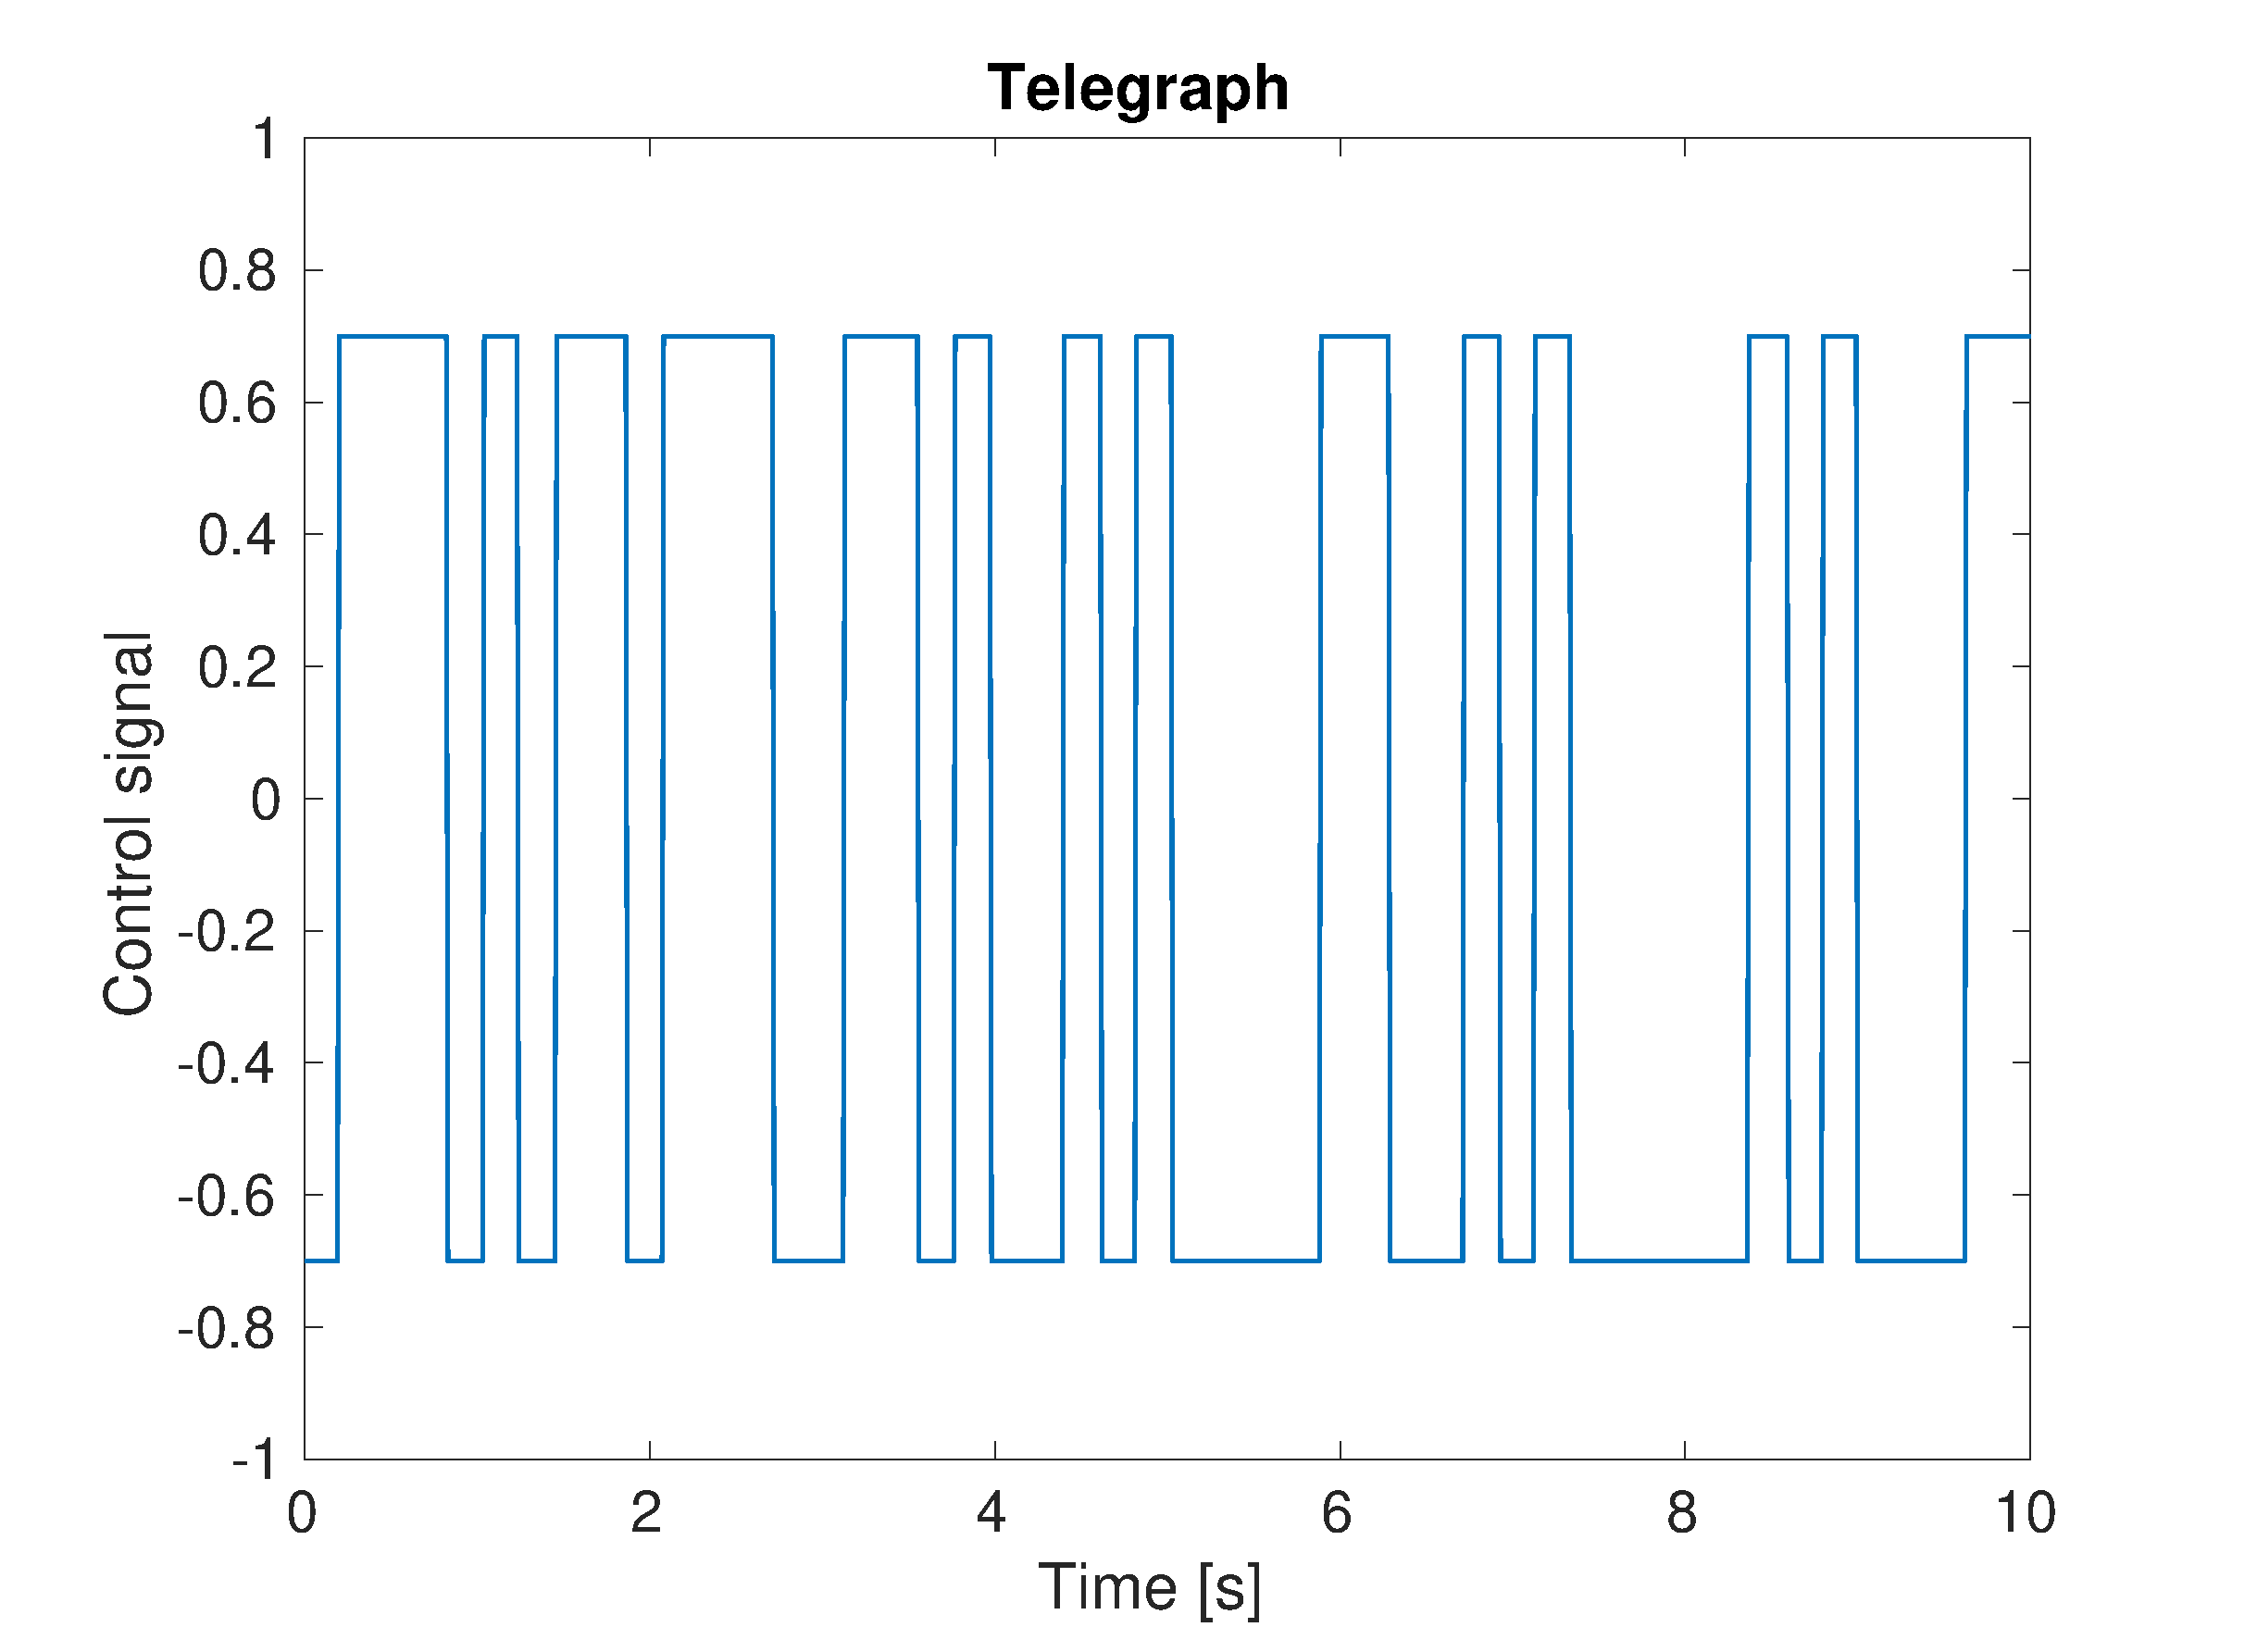
\includegraphics[width=0.8\textwidth]{telegraph}
\caption{An example of a telegraph signal which was sent to a thruster during data collection experiments.}
\label{fig:telegraph}
\end{figure}

\begin{figure}[htbp]
  \centering
  \subfloat[][\label{fig:p_pqTest}Excitation in $p$ during $p$ and $q$ test.]{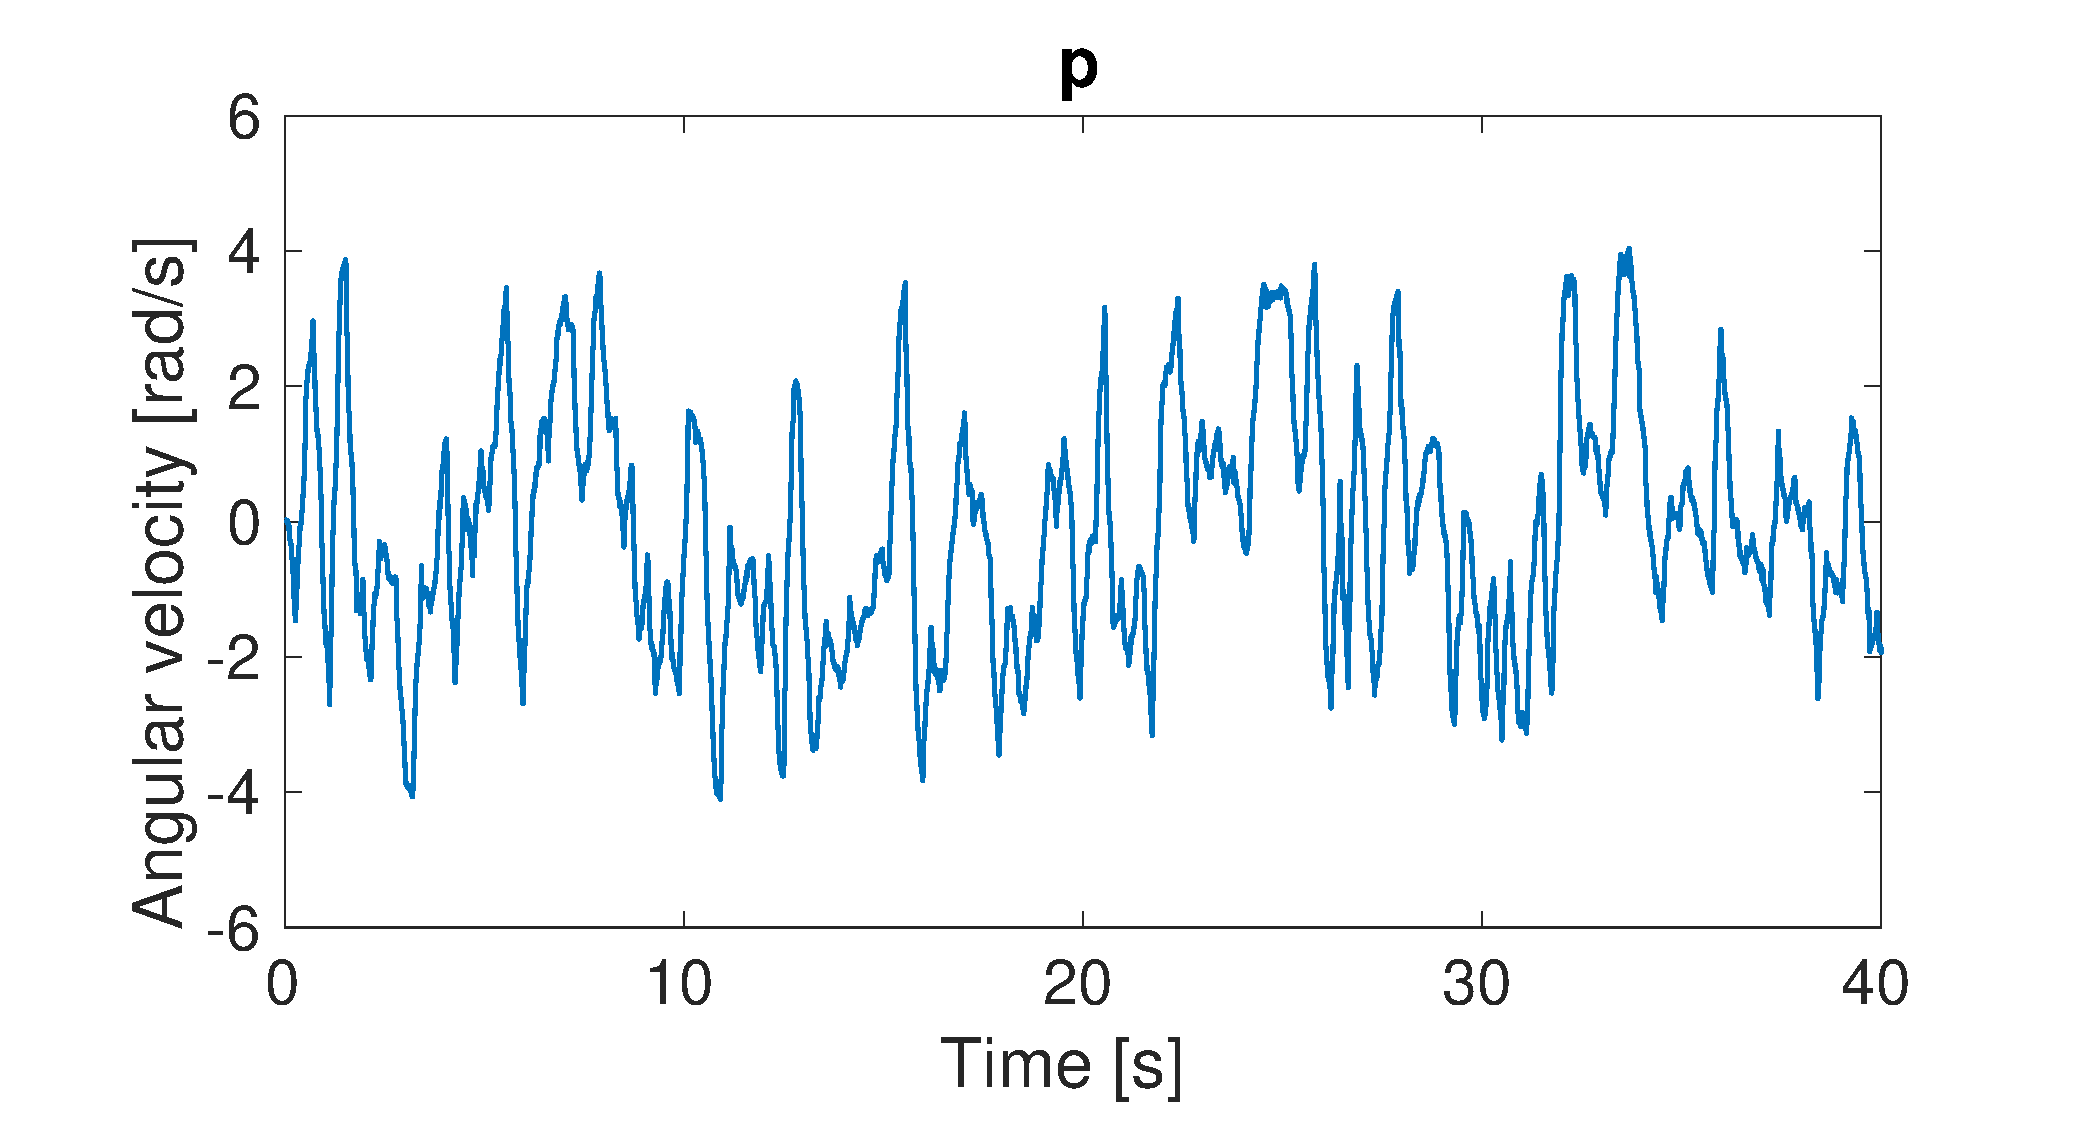
\includegraphics[width=0.7\textwidth]{p_pq_test}}
  \qquad
  \subfloat[][\label{fig:q_pqTest}Excitation in $q$ during $p$ and $q$ test.]{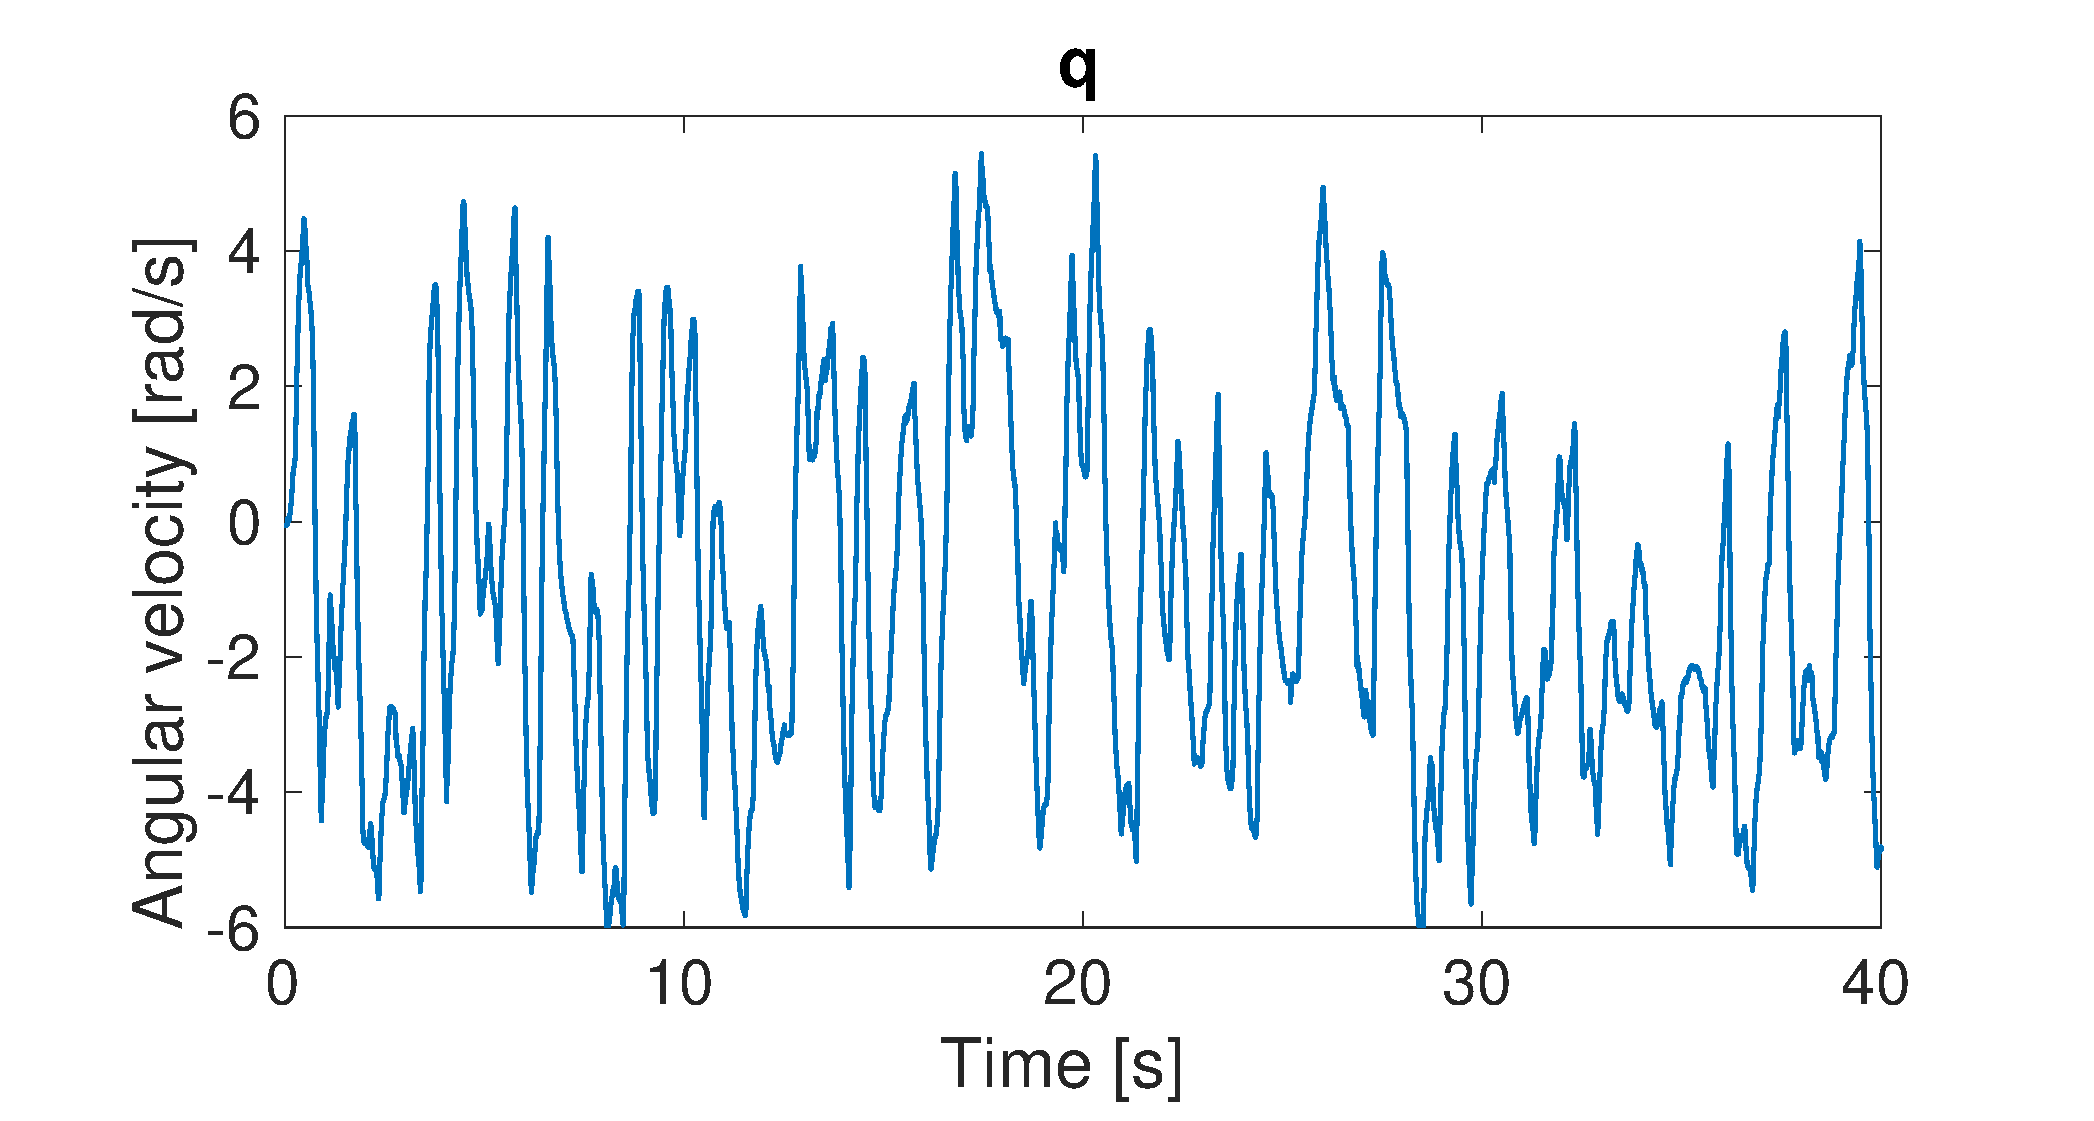
\includegraphics[width=0.7\textwidth]{q_pq_test}}
  \\
  \subfloat[][\label{fig:r_pqTest}Excitation in $r$ during $p$ and $q$ test.]{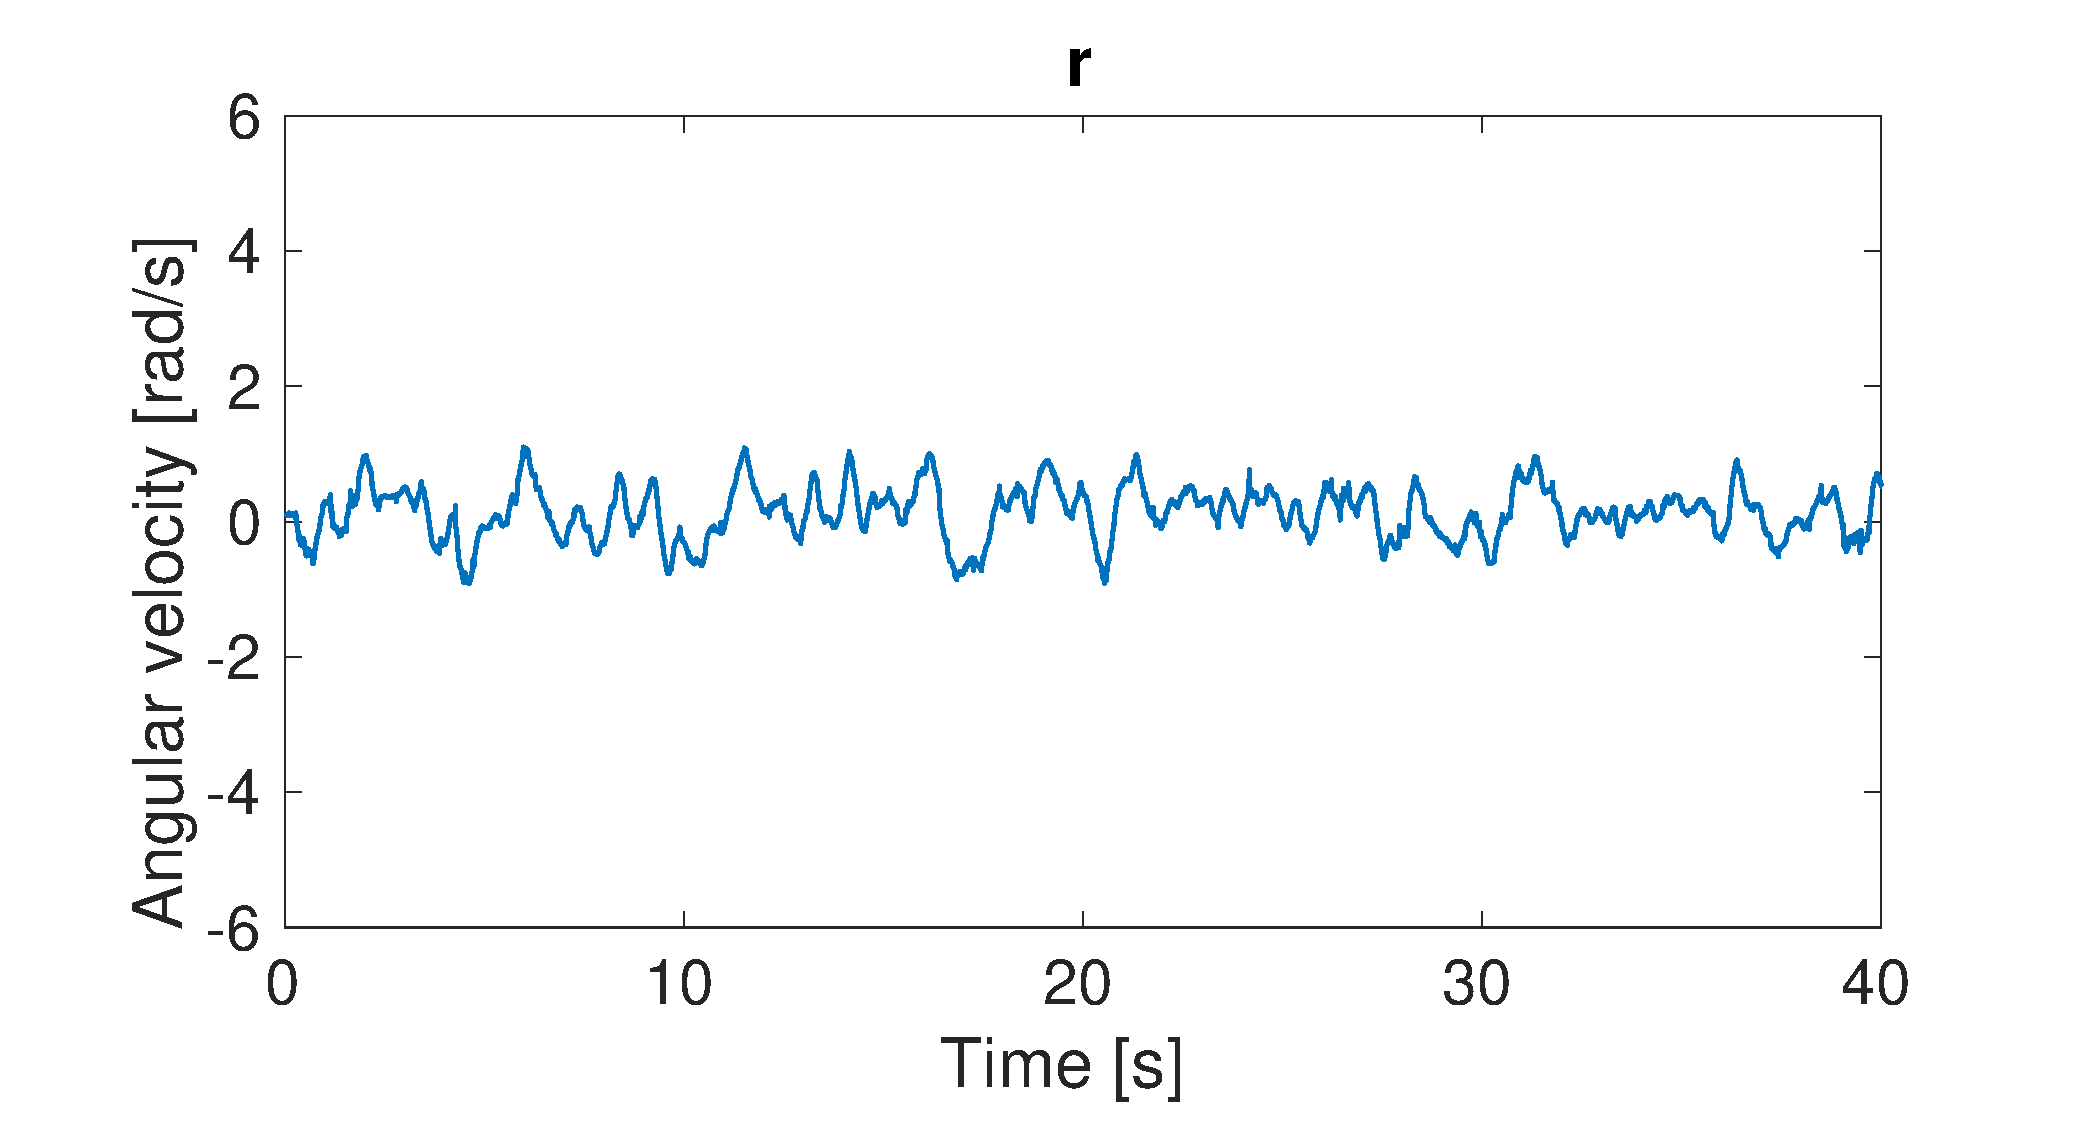
\includegraphics[width=0.7\textwidth]{r_pq_test}}
  \caption{\label{fig:pqTest}%
 Plots of excitation of the three angular velocities $p$, $q$ and $r$ from a test intended to mainly excite $p$ and $q$. Note that the amplitude in $r$ is four times smaller than that of $p$ and $q$.}
\end{figure}

\begin{figure}[htbp]
  \centering
  \subfloat[][\label{fig:p_rTest}Excitation in $p$ during $r$ test.]{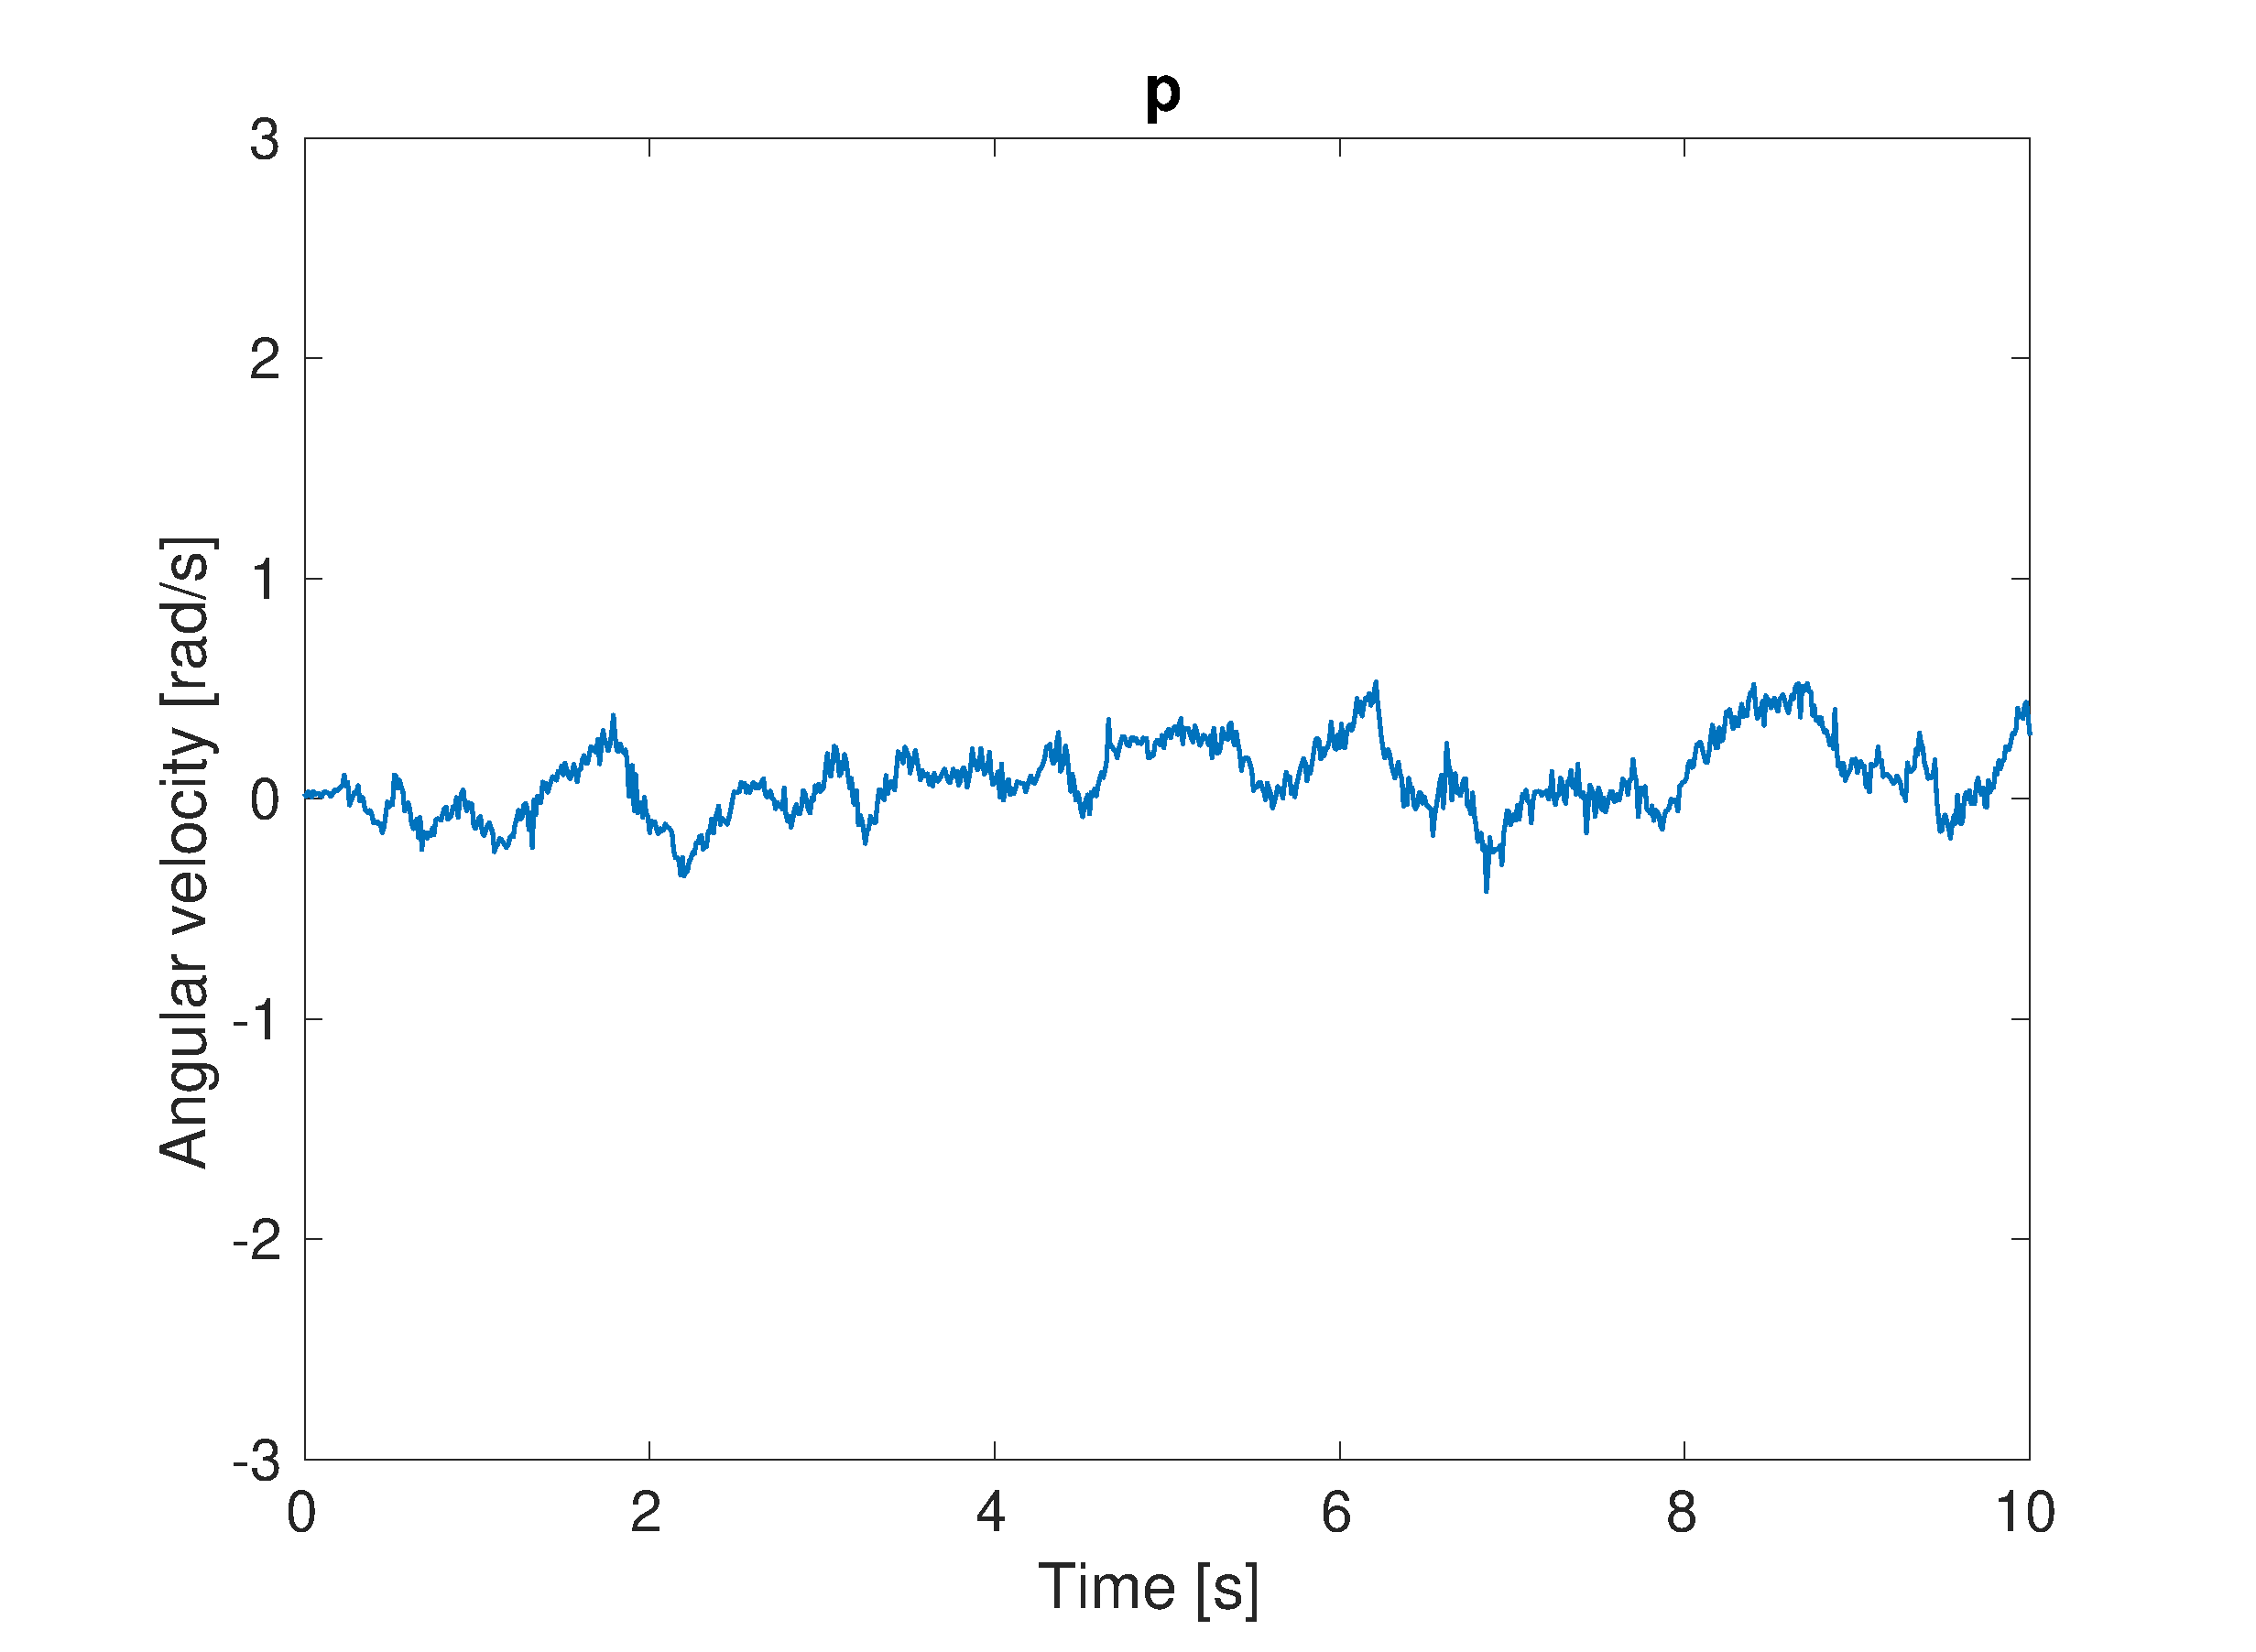
\includegraphics[width=0.7\textwidth]{p_r_test}}
  \qquad
  \subfloat[][\label{fig:q_rTest}Excitation in $q$ during $r$ test.]{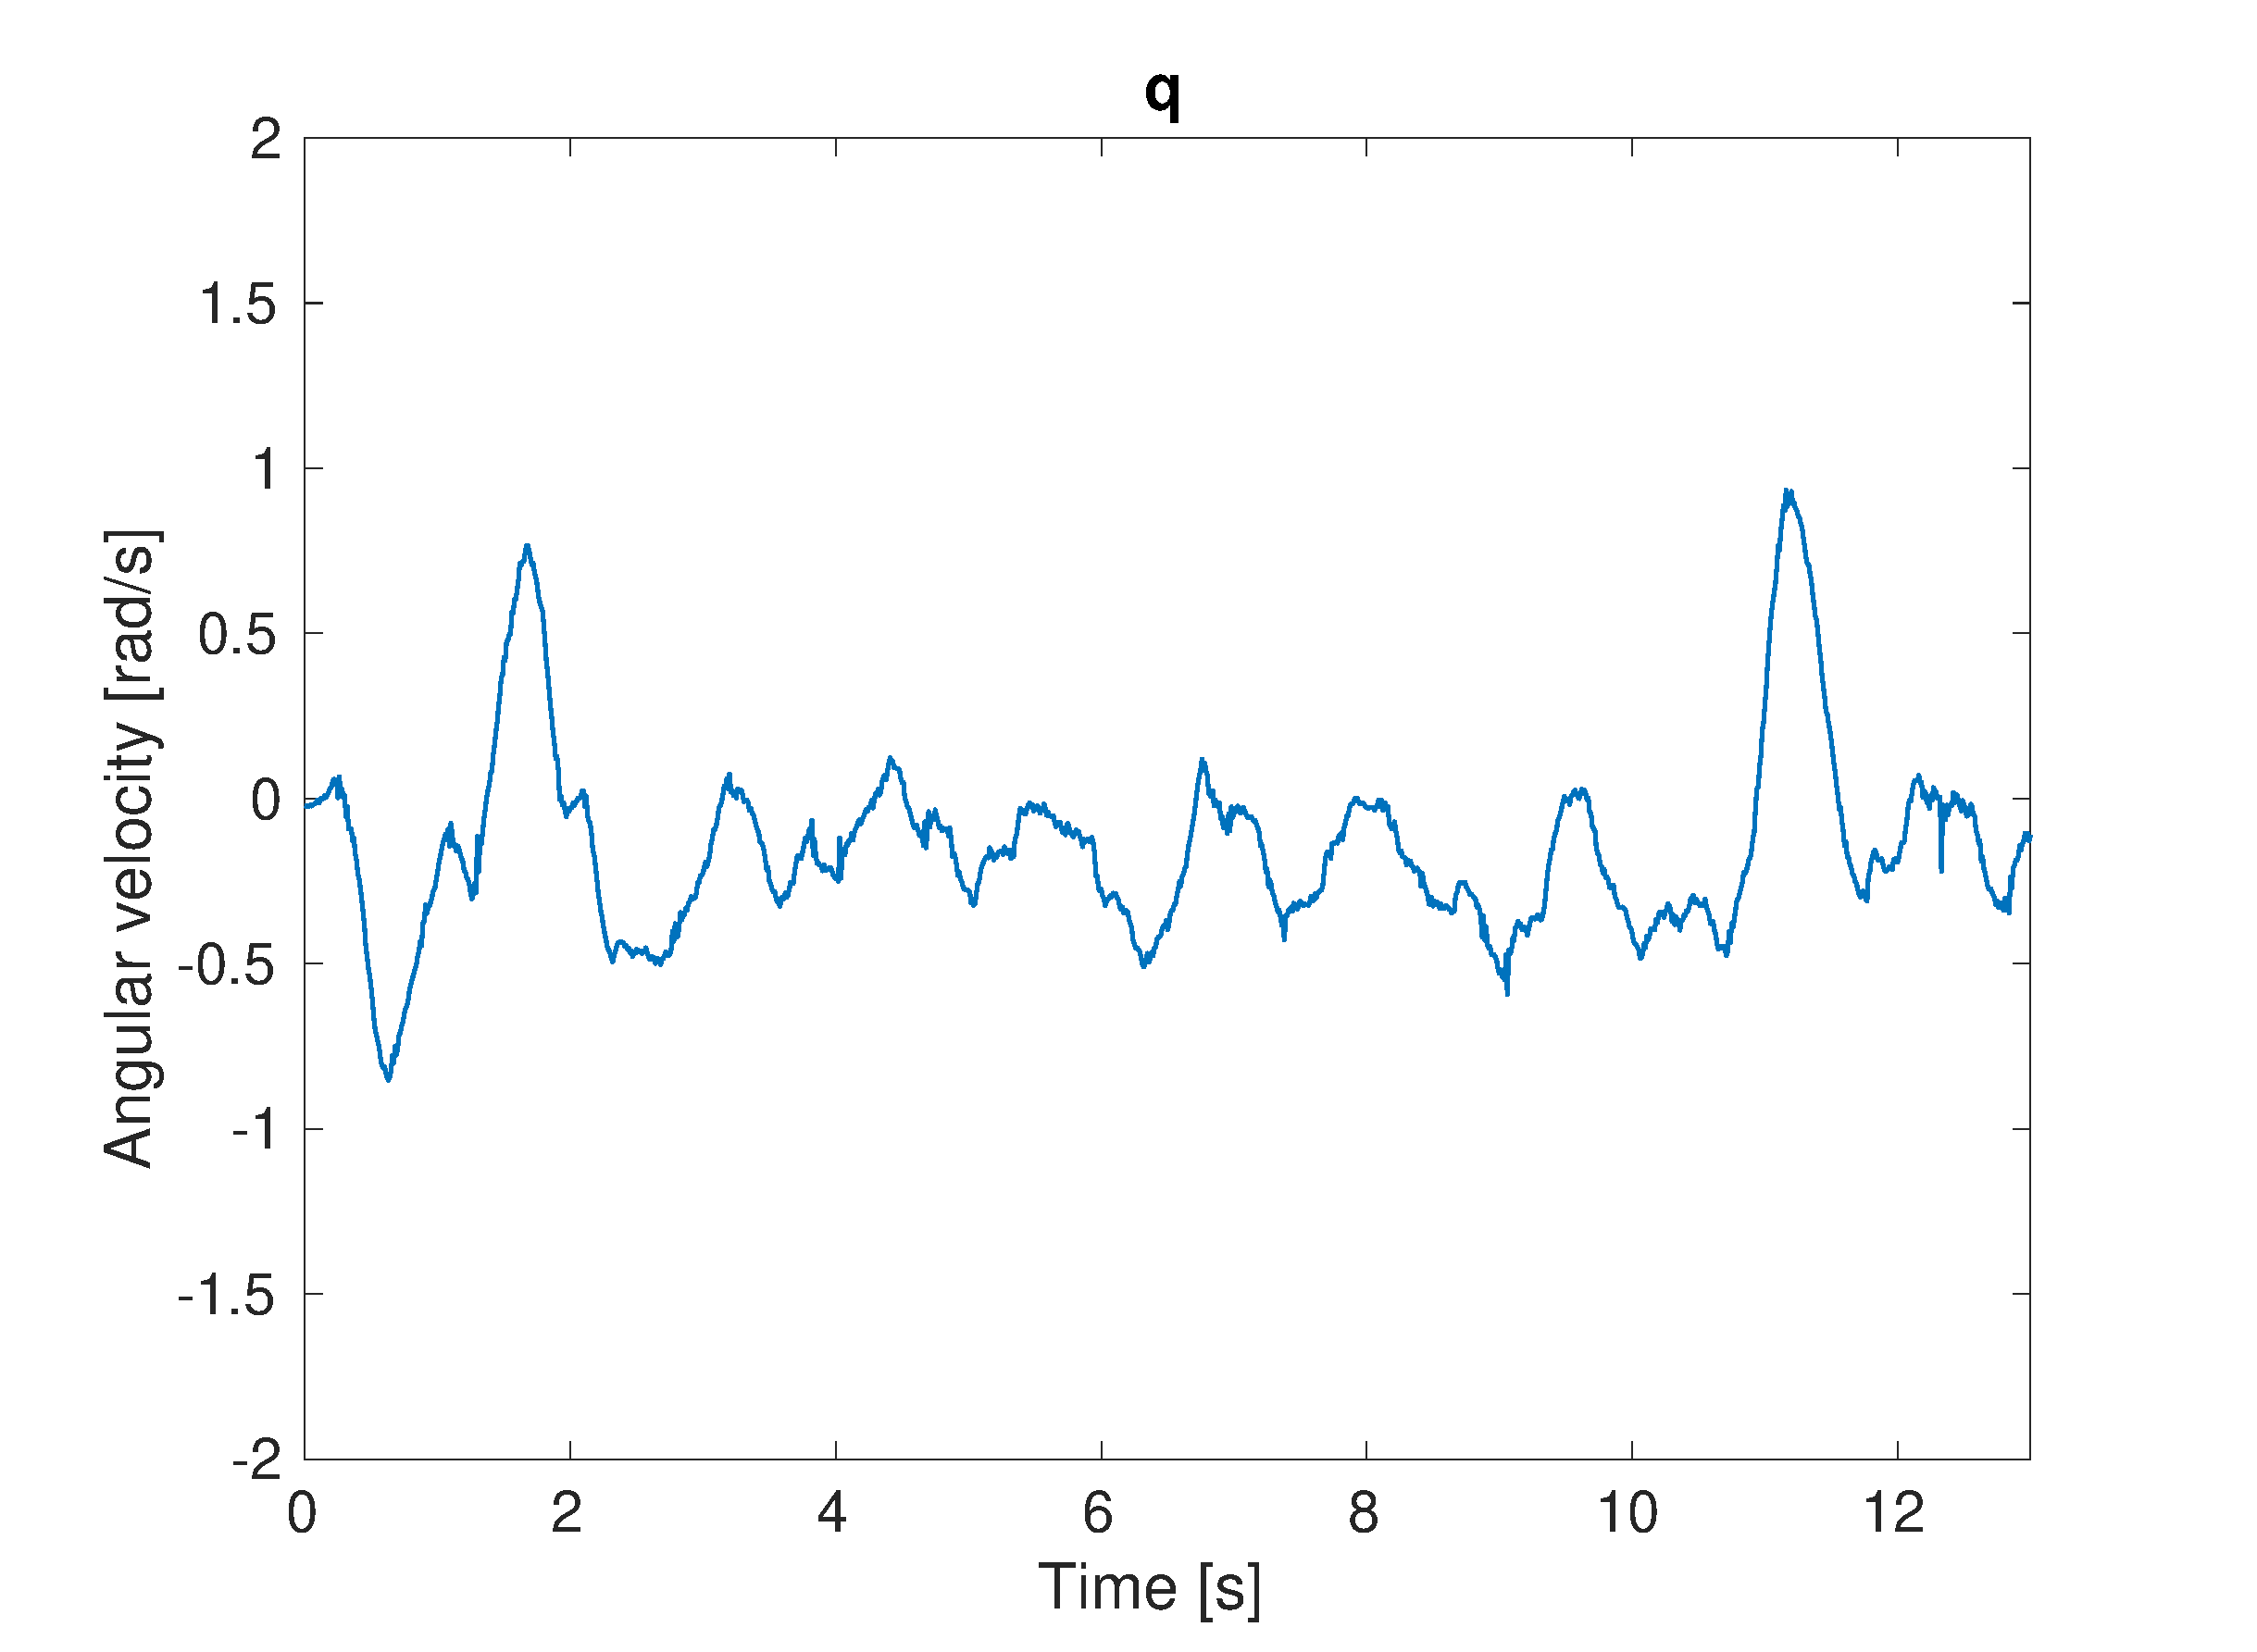
\includegraphics[width=0.7\textwidth]{q_r_test}}
  \\
  \subfloat[][\label{fig:r_rTest}Excitation in $r$ during $r$ test.]{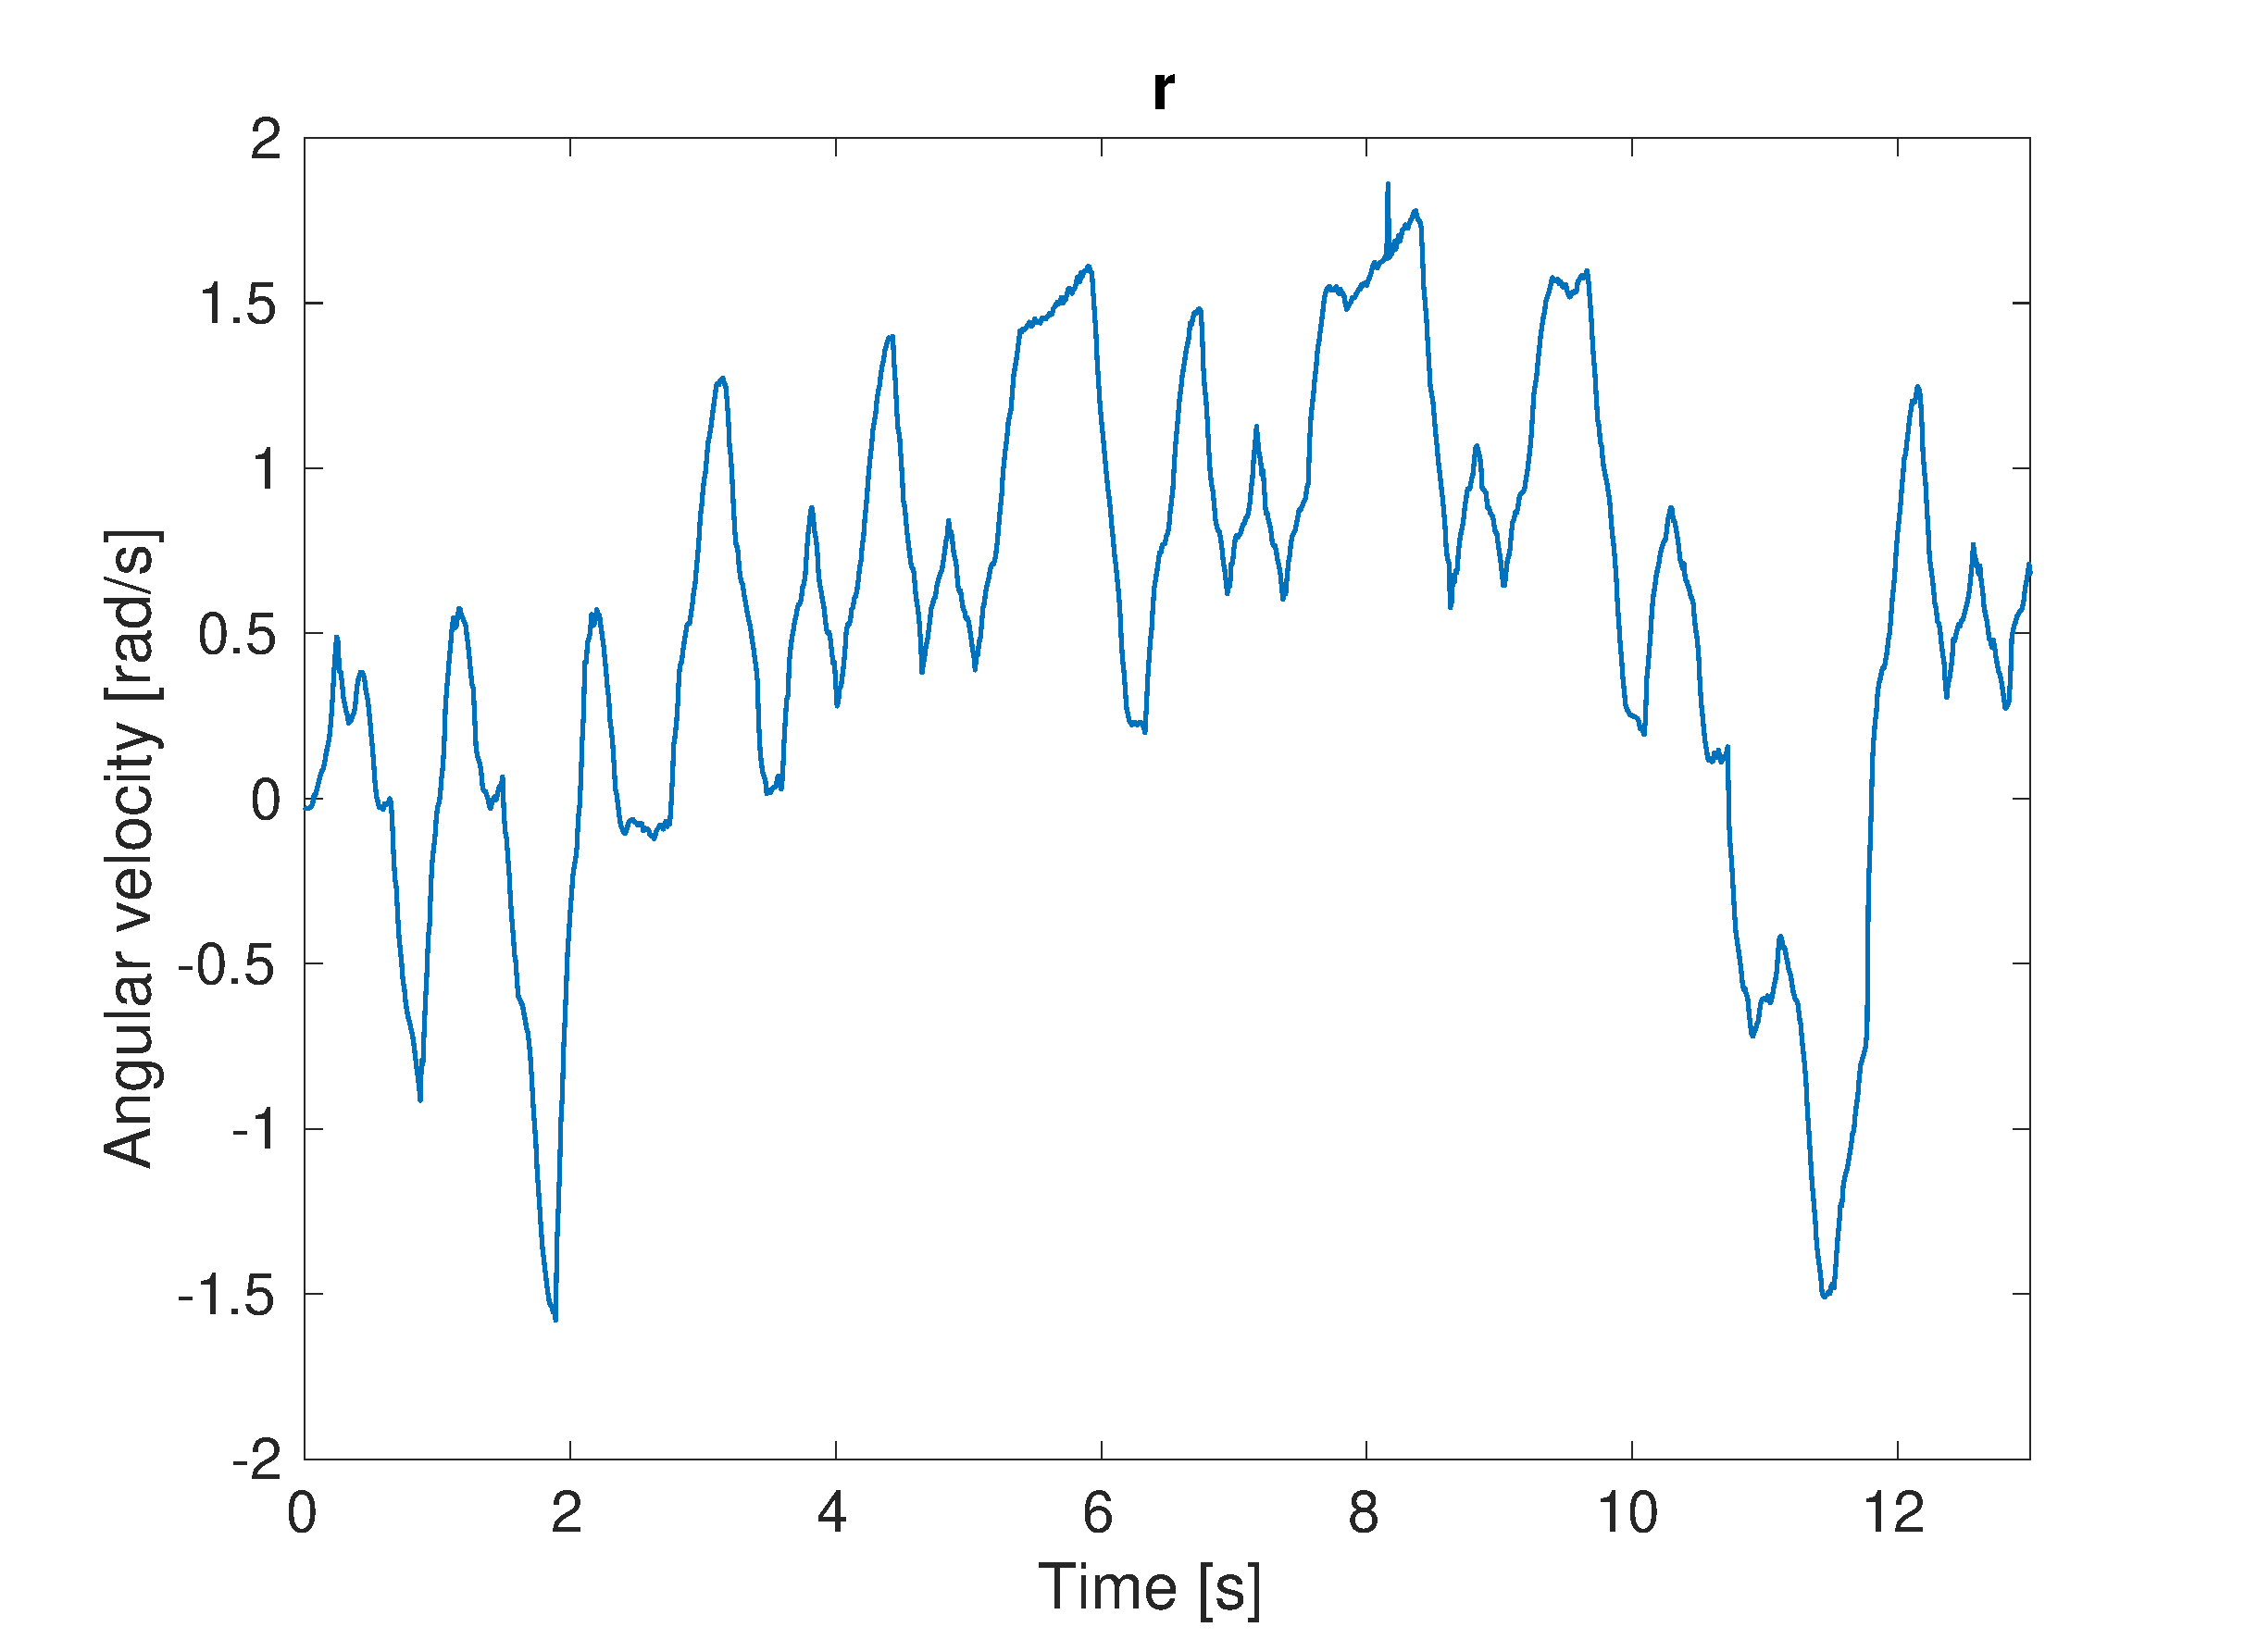
\includegraphics[width=0.7\textwidth]{r_r_test}}
  \caption{\label{fig:rTest}%
 Plots of excitation of the three angular velocities $p$, $q$ and $r$ from a test intended to mainly excite $r$. Note that the amplitude in $r$ is approximately two times larger than that of $p$ and $q$.}
\end{figure}

%%%%%%%%%%%%%%%%%%%%%%%%%%%%%%%%%%%%%%%%%%%%%%%%%%%%%%%%%%%
\section{Results}
In this section will the results from the different parameter estimation methods be presented. Estimated parameter values and the fit of the models compared to validation data are presented.

\subsection{Prediction-Error Method}
Using the model structure \eqref{eq:pq_dot_decouple} and \eqref{eq:r_dot_decouple} with the reparametrisation done in \eqref{eq:quatModel} and using the estimated angles as inputs and angular velocities as outputs gave the following model structure to be estimated
\begin{equation}
\etaVectordot = f(\nuVector, \hat{\etaVector}, \tauVector),
\end{equation}
and
\begin{equation}
\boldsymbol{y} = \nuVector
\end{equation}
where $\hat{\etaVector}$ are the estimated Euler angles from the sensor fusion.
The result of the estimation can be seen in \Tableref{tab:ResultEstimAngular}. The estimation used two datasets as estimation data and used one dataset for validation data. The fit of the model compared to validation data can be seen in \Figureref{fig:velocityCompareCong}.

\begin{table}[hbp]
  \centering
  \caption{\label{tab:ResultEstimAngular}%
    The estimated parameters from the prediction-error method using the estimated angles as inputs and angular velocities as outputs. During estimation was $\distance{z}{6} = 0.11$.}
  \begin{tabular}{l l p{0.25\linewidth}}
    \toprule%
    \textbf{Notation}  & \textbf{Starting Value} & \textbf{Estimated Value} \\
    \otoprule%   
    % Parameters that will be estimated
	$z_B$               & -0.01 	\meter 						& -0.017849 \meter\\
    $\Kp$               & -1   	\kilogram\usk\meter\squared 	& -1.3275  	\kilogram\usk\meter\squared\\
    $\Kpabsp$           & -1  	\kilogram\usk\meter\squared	& 	0  		\kilogram\usk\meter\squared\\
    $\Mq$               & -1  	\kilogram\usk\meter\squared	& -1.1925	\kilogram\usk\meter\squared\\
    $\Mqabsq$           & -1  	\kilogram\usk\meter\squared	& -0.10935  \kilogram\usk\meter\squared\\
    $\Nr$               & -1  	\kilogram\usk\meter\squared	&  -2.7838 	\kilogram\usk\meter\squared\\
    $\Nrabsr$           & -1  	\kilogram\usk\meter\squared	& -0.67509	\kilogram\usk\meter\squared\\
    $A_p$               & 1.5 	\kilogram\usk\meter\squared	& 0.32545  	\kilogram\usk\meter\squared\\
    $B_q$               & 1.5 	\kilogram\usk\meter\squared	& 0.37526 	\kilogram\usk\meter\squared\\
    $C_r$               & 1.5 	\kilogram\usk\meter\squared	& 0.95462	\kilogram\usk\meter\squared\\
    \bottomrule%
  \end{tabular}
\end{table}  

\begin{figure}[tbp]
  \centering
  \subfloat[][\label{fig:velocityCompareCongp}Comparison between a simulated model without reparametrisation and validation data in the $p$.]{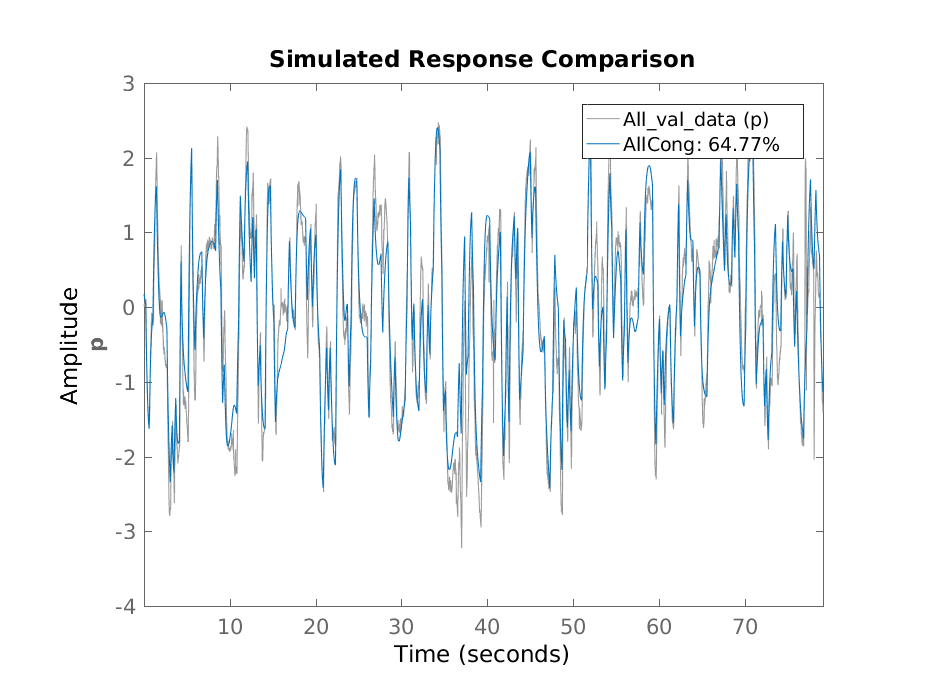
\includegraphics[width=0.5\textwidth]{velocityCompareCongp}}
  \qquad
  \subfloat[][\label{fig:velocityCompareCongq}Comparison between a simulated model without reparametrisation and validation data in the $q$.]{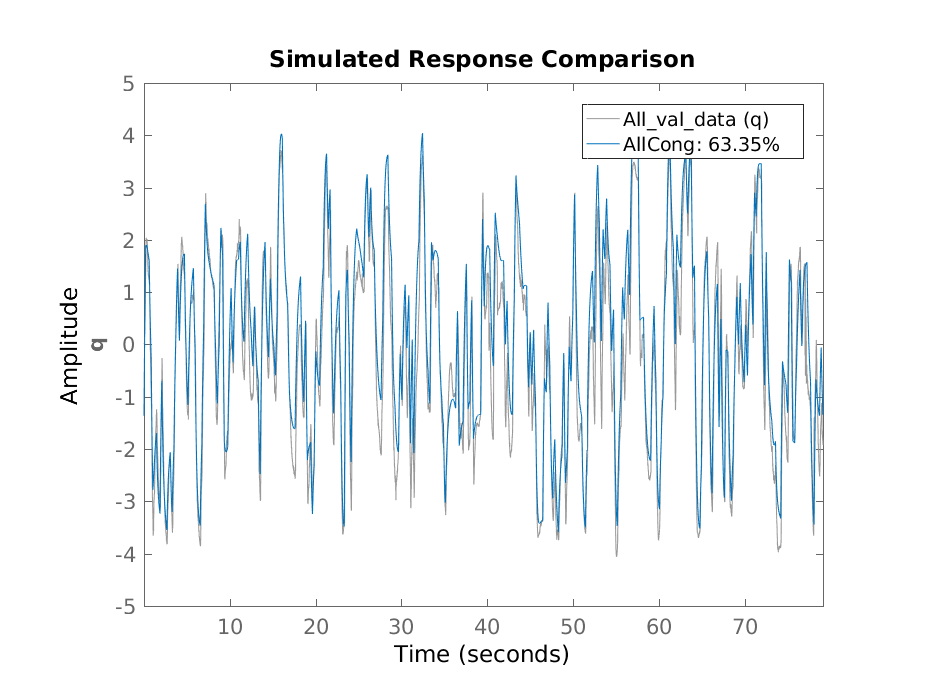
\includegraphics[width=0.5\textwidth]{velocityCompareCongq}}
  \\
  \subfloat[][\label{fig:velocityCompareCongr}Comparison between a simulated model without reparametrisation and validation data in the $r$.]{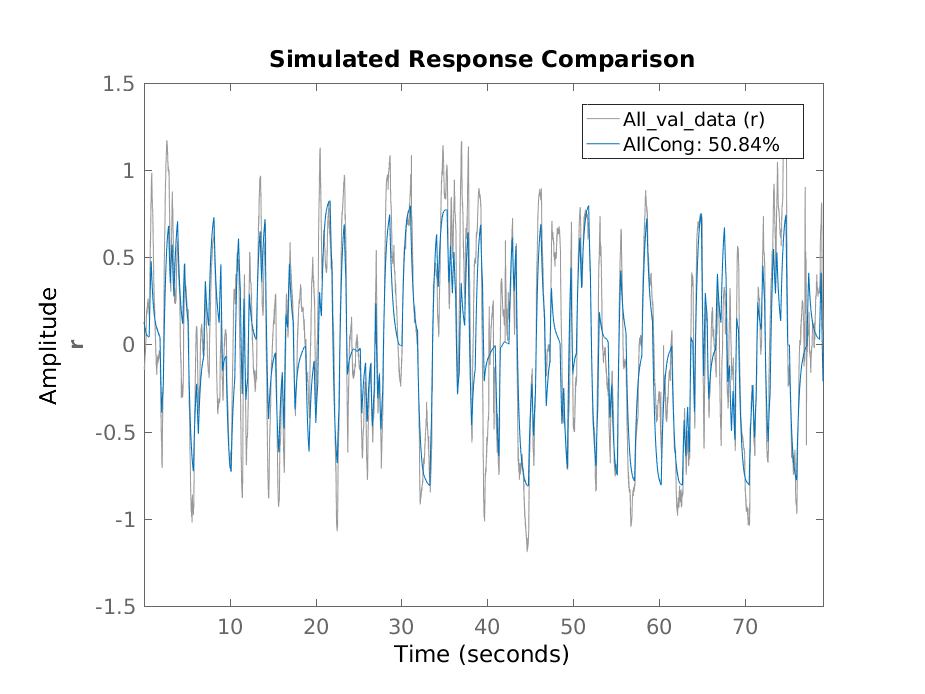
\includegraphics[width=0.5\textwidth]{velocityCompareCongr}}
  \caption{\label{fig:velocityCompareCong}%
    Comparison of simulation of the attitude model against validation data using the estimated angels as inputs and angular velocities as outputs.}
\end{figure}

Using the model structure defined in \eqref{eq:pq_dot_decouple} with angular velocities and linear acceleration as outputs resulted in the model structure
\begin{equation}
\etaVectordot = J(\etaVector) \nuVector,
\end{equation}
\begin{equation}
\dot{\nuVector} =  f(\etaVector, \nuVector, \tauVector)
\end{equation}
with 
\begin{equation}
\boldsymbol{y} = \begin{pmatrix}
\etaVector \\
\boldsymbol{a}
\end{pmatrix}
\end{equation}
where $\boldsymbol{a}$ is the linear acceleration in the \abbrROV frame.
The estimated parameter values obtained using this model structure can be seen in \Tableref{tab:ResultangVellz60} and \Tableref{tab:ResultangVellz}. The estimation was done with four datasets and two datasets was used for validation.

\begin{table}[hbp]
  \centering
  \caption{\label{tab:ResultangVellz60}%
    The estimated parameters from the prediction-error method using angular velocities and linear acceleration as outputs with $\distance{z}{6} = 0$.}
  \begin{tabular}{l l p{0.25\linewidth}}
    \toprule%
    \textbf{Notation}  & \textbf{Starting Value} & \textbf{Estimated Value} \\
    \otoprule%   
    % Parameters that will be estimated
	$z_B$               & -0.01 	\meter 						& -0.010625 \meter\\
    $\Kp$               & -1   	\kilogram\usk\meter\squared 	& -2.4079  	\kilogram\usk\meter\squared\\
    $\Kpabsp$           & -1  	\kilogram\usk\meter\squared	& 	0  		\kilogram\usk\meter\squared\\
    $\Mq$               & -1  	\kilogram\usk\meter\squared	& -0.14202  \kilogram\usk\meter\squared\\
    $\Mqabsq$           & -1  	\kilogram\usk\meter\squared	& -0.80813  \kilogram\usk\meter\squared\\
    $\Nr$               & -1  	\kilogram\usk\meter\squared	& -2.4975 	\kilogram\usk\meter\squared\\
    $\Nrabsr$           & -1  	\kilogram\usk\meter\squared	& -1.7811	\kilogram\usk\meter\squared\\
    $A_p$               & 1.5 	\kilogram\usk\meter\squared	& 0.55821  	\kilogram\usk\meter\squared\\
    $B_q$               & 1.5 	\kilogram\usk\meter\squared	& 0.49512 	\kilogram\usk\meter\squared\\
    $C_r$               & 1.5 	\kilogram\usk\meter\squared	& 1.026 		\kilogram\usk\meter\squared\\
    \bottomrule%
  \end{tabular}
\end{table}

The fit of the model using the estimated parameters, with $\distance{z}{6} = 0$, can be viewed in \Figureref{fig:angVelCompare} and the fit of the model with $\distance{z}{6} = 0.11$ can be seen in \Figureref{fig:angVelComparelz6}. 

\begin{figure}[tbp]
  \centering %simulation of estimation. Estimator given wrong initial state
  \subfloat[][\label{fig:angVelComparep}Comparison of angular velocity around the \abbrROV's x-axis between validation data and the simulated model.]{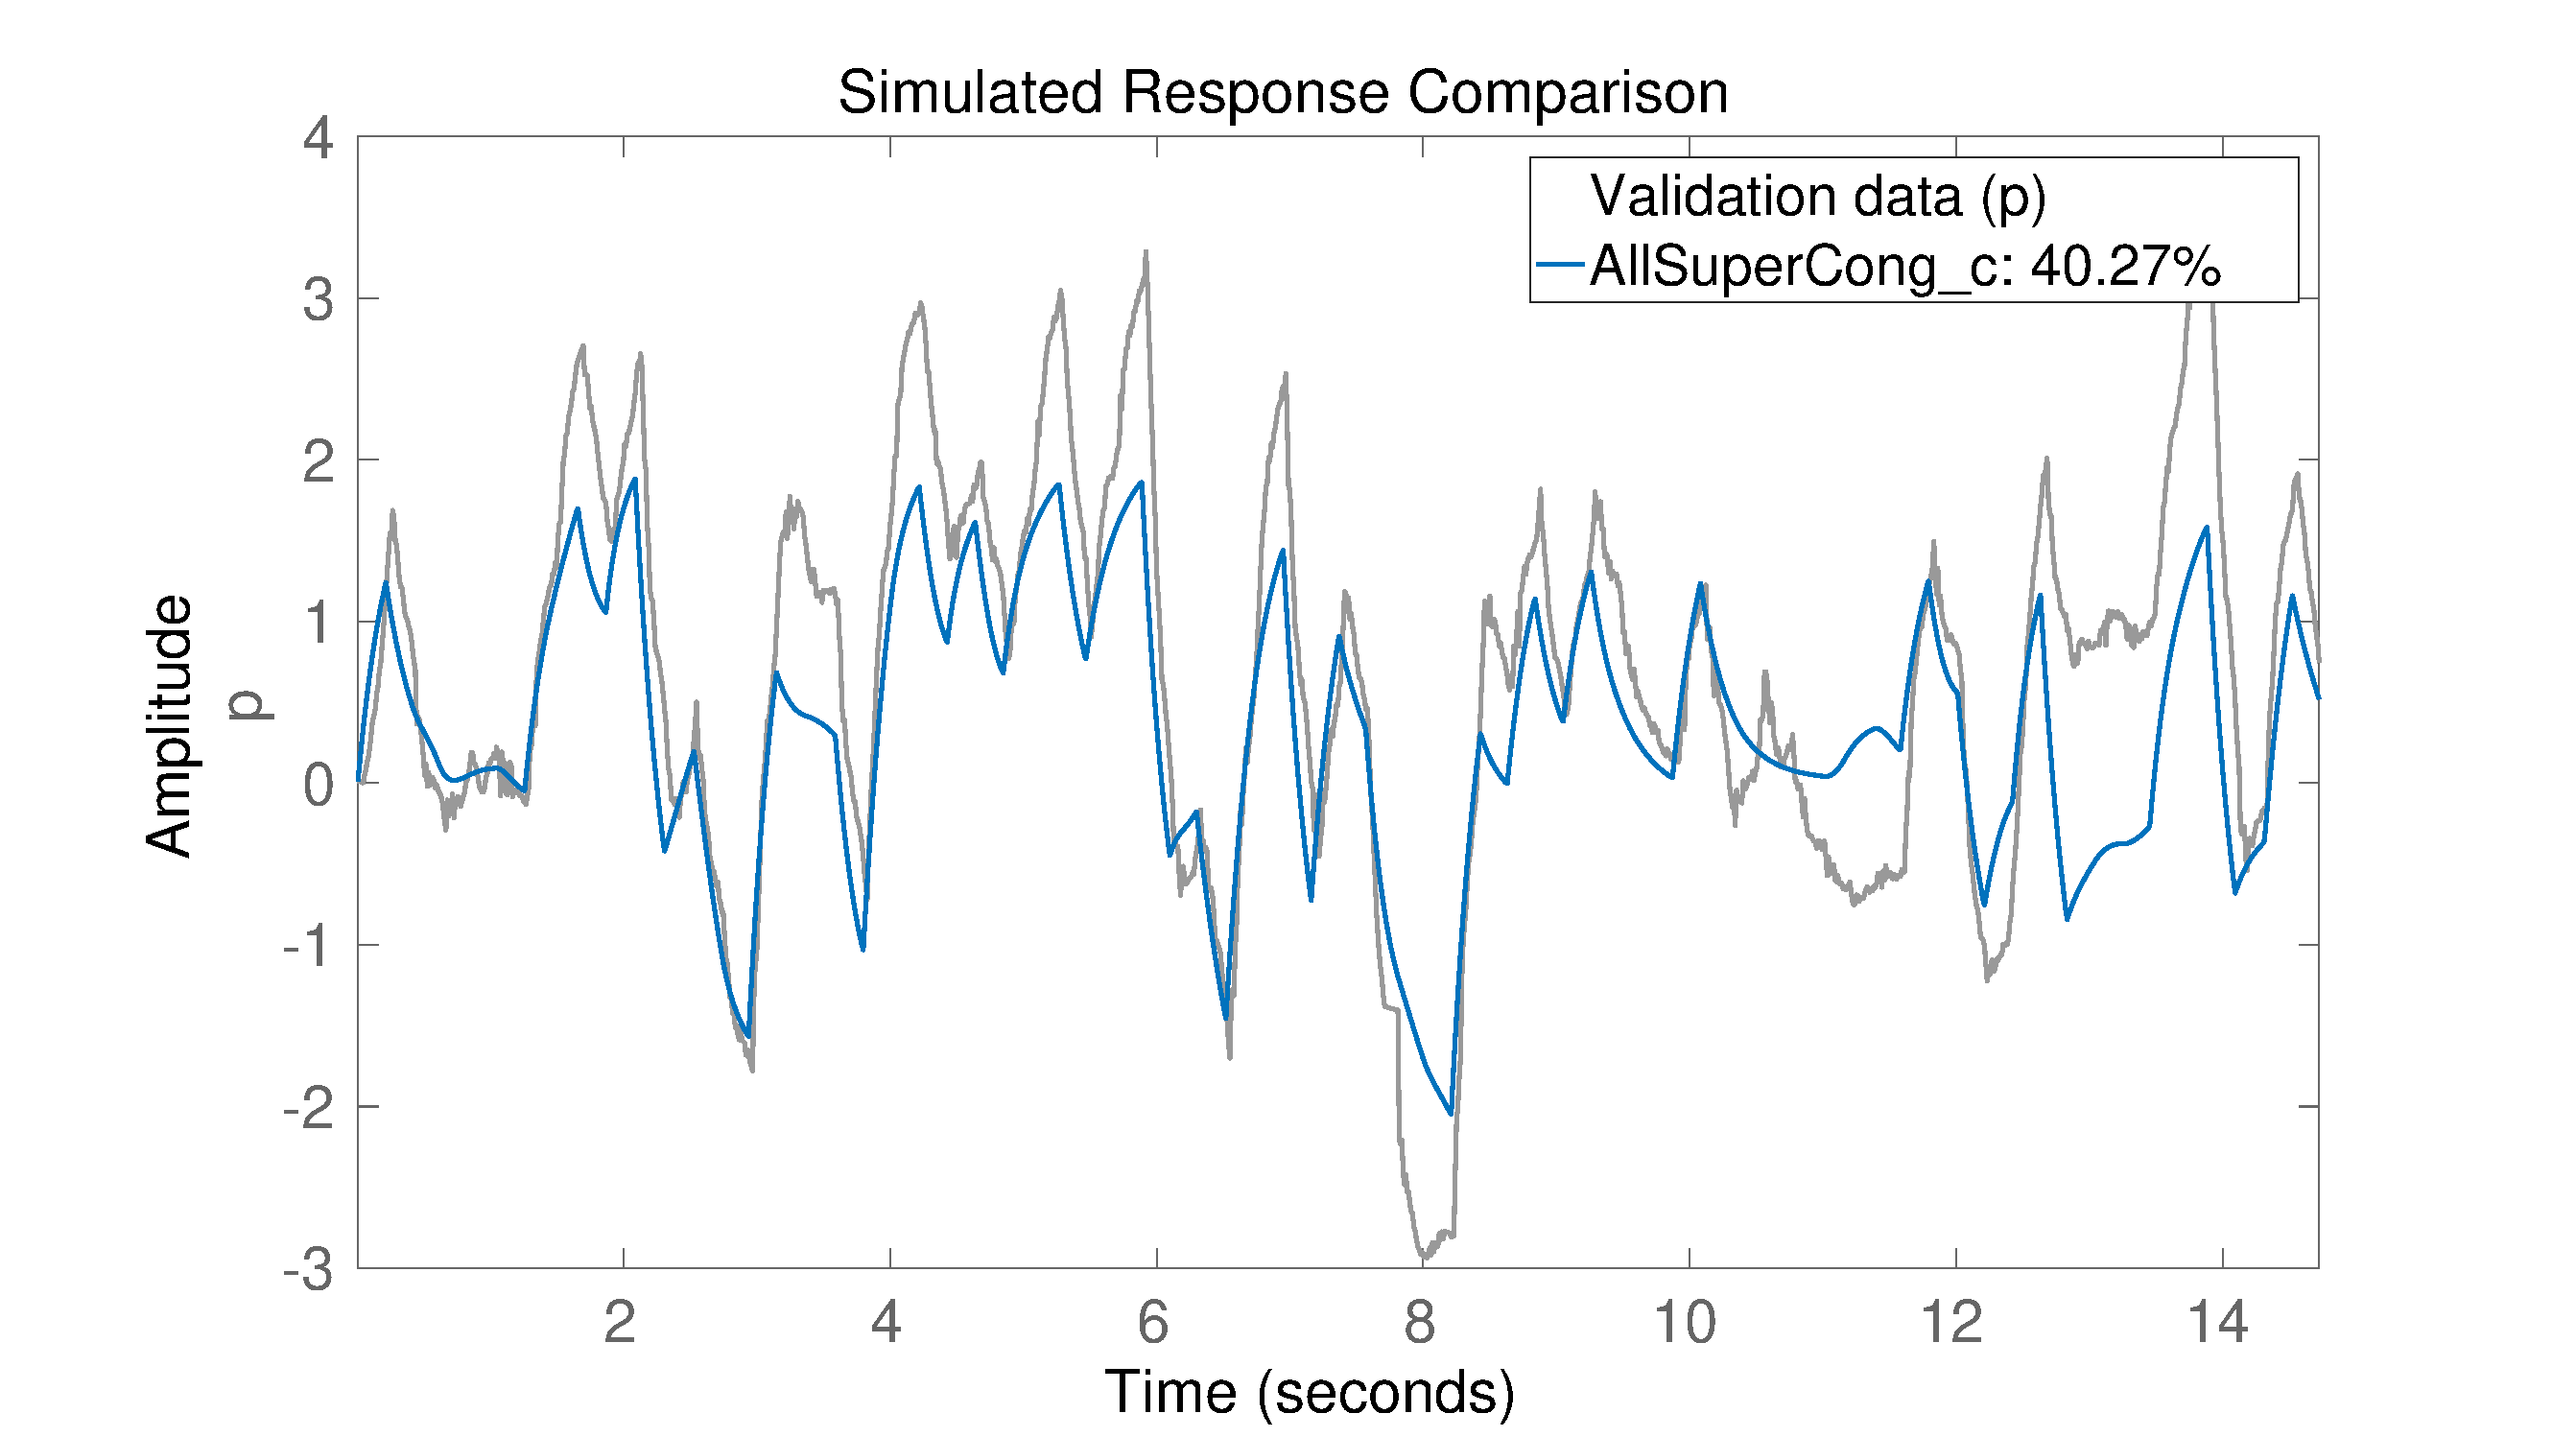
\includegraphics[width=0.4\textwidth]{angVelComparep}}
  \qquad
  \subfloat[][\label{fig:angVelCompareq}Comparison of angular velocity around the \abbrROV's y-axis between validation data and the simulated model.]{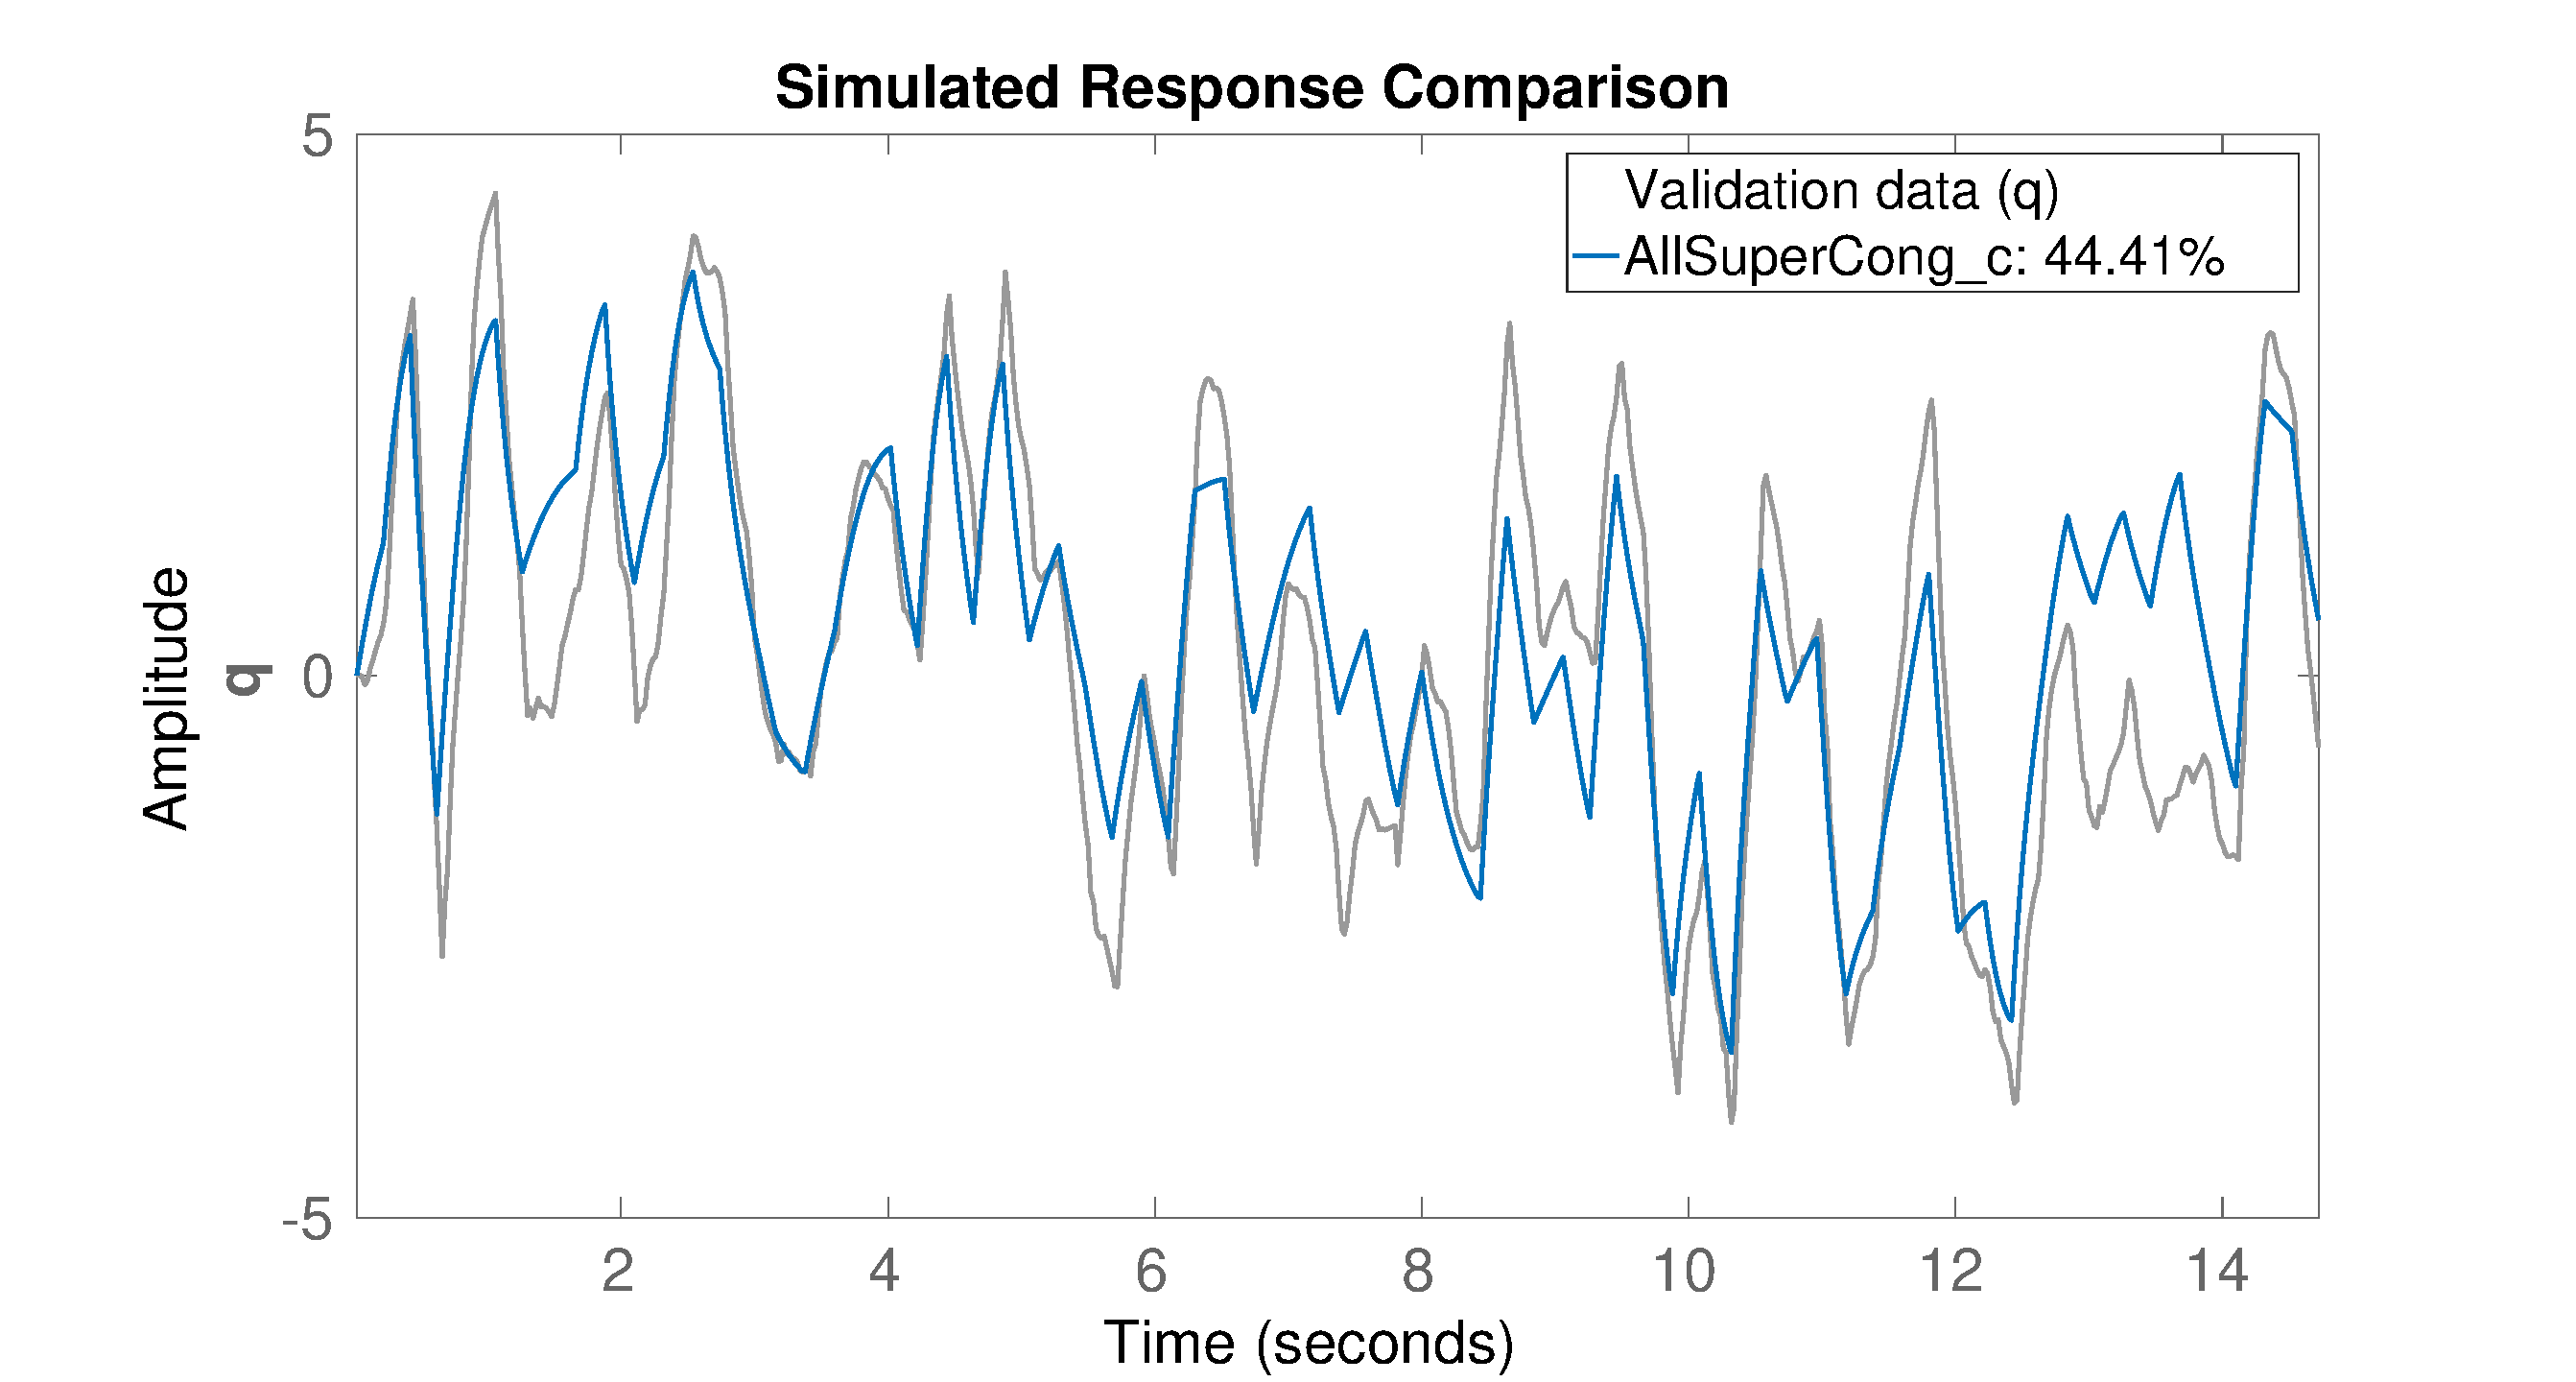
\includegraphics[width=0.4\textwidth]{angVelCompareq}}
  \qquad
  \subfloat[][\label{fig:angVelComparer}Comparison of angular velocity around the \abbrROV's z-axis between validation data and the simulated model.]{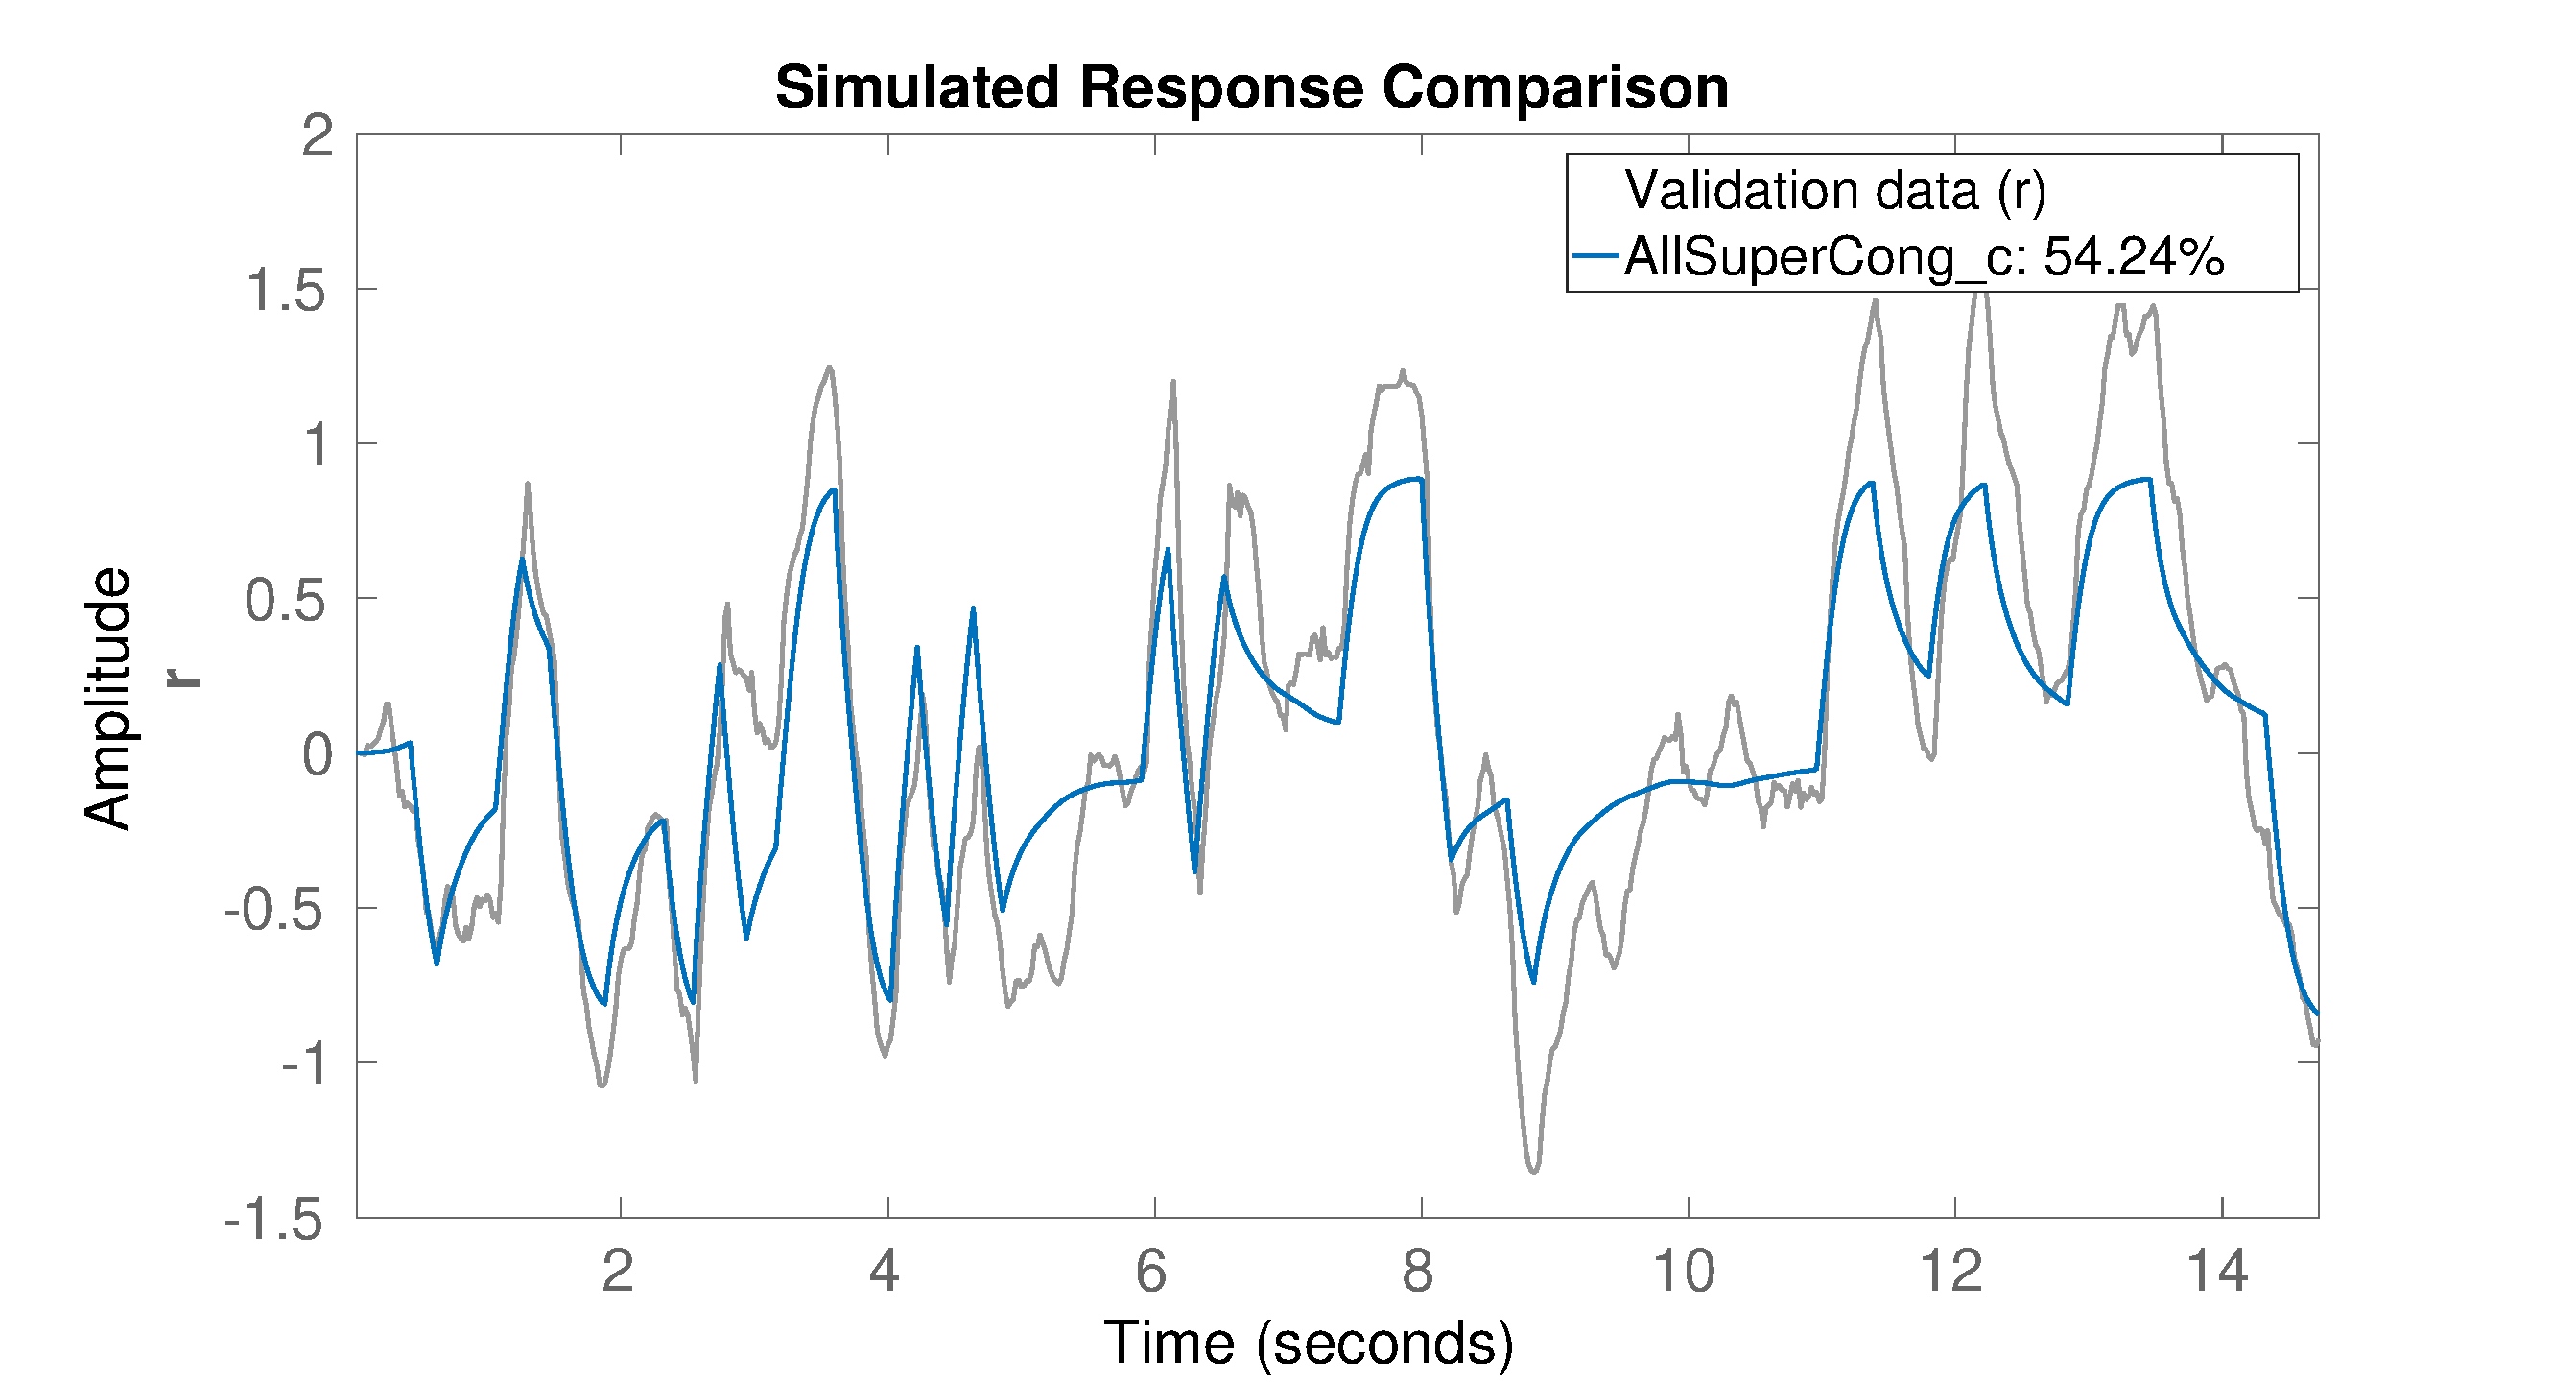
\includegraphics[width=0.4\textwidth]{angVelComparer}}
    \qquad
  \subfloat[][\label{fig:linAccComparex}Comparison of linear acceleration in the \abbrROV's x-axis between validation data and the simulated model.]{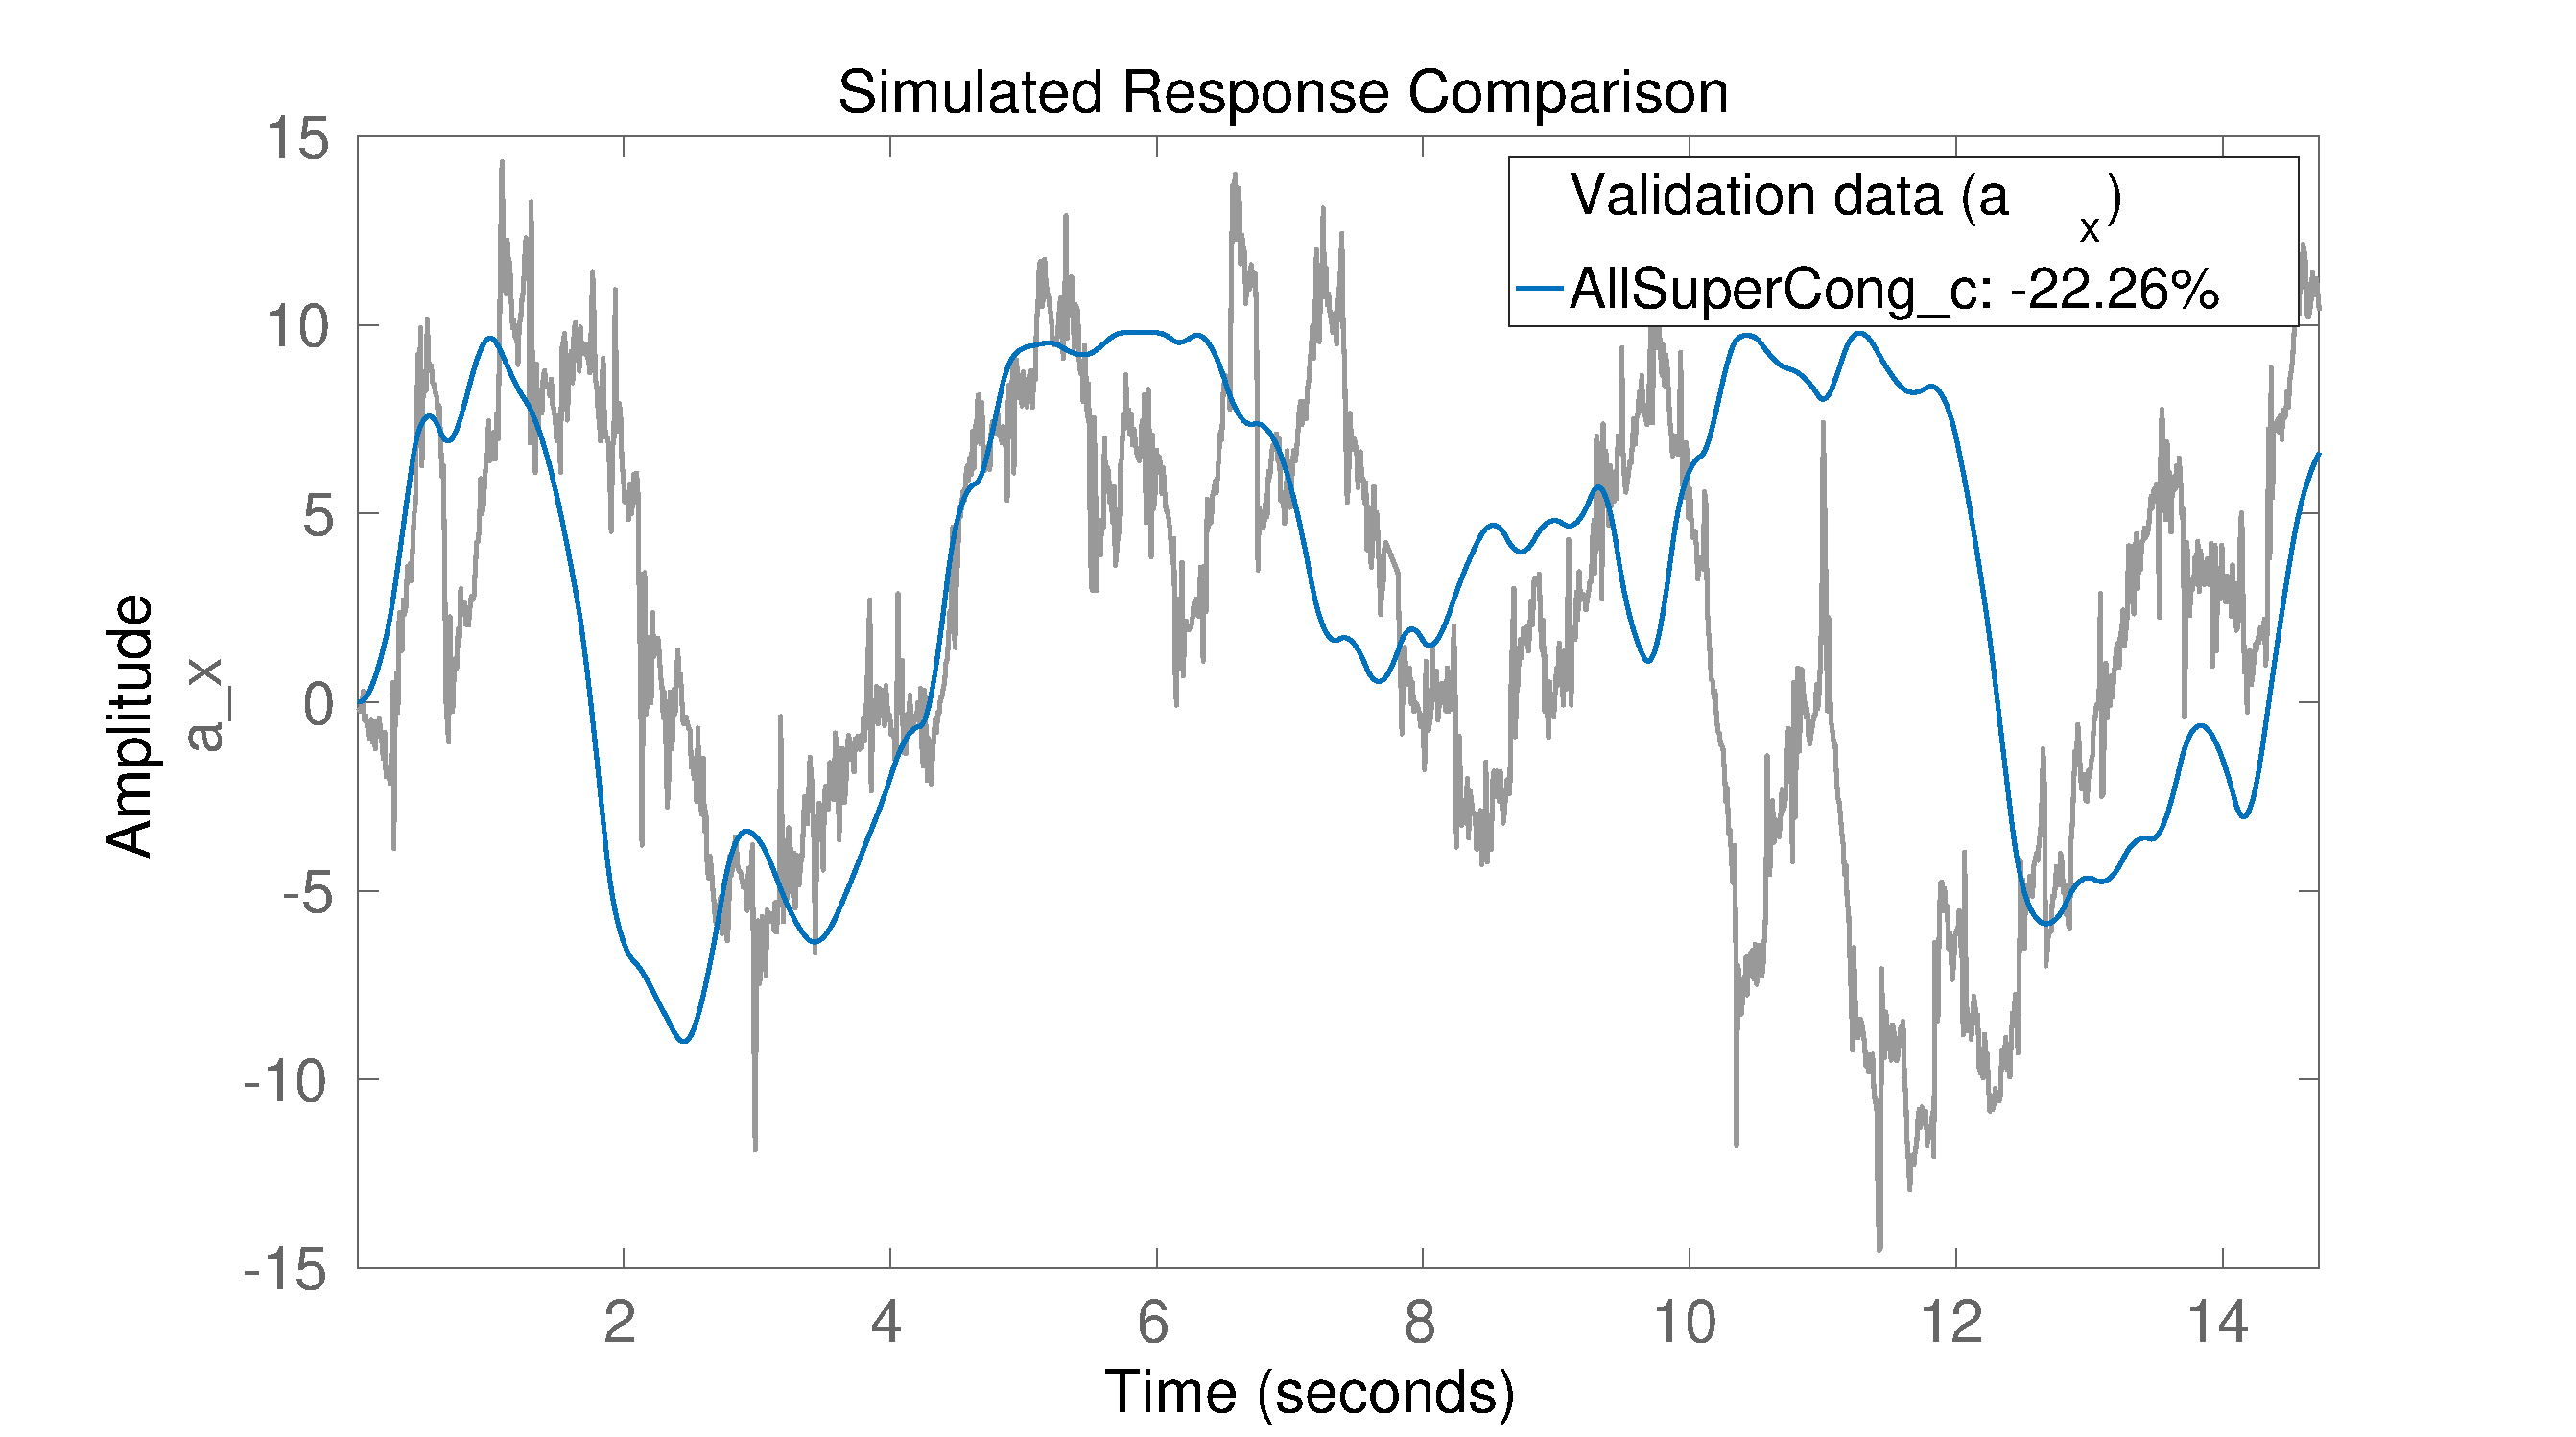
\includegraphics[width=0.4\textwidth]{linAccComparex}}
    \qquad
  \subfloat[][\label{fig:linAccComparey}Comparison of linear acceleration in the \abbrROV's y-axis between validation data and the simulated model.]{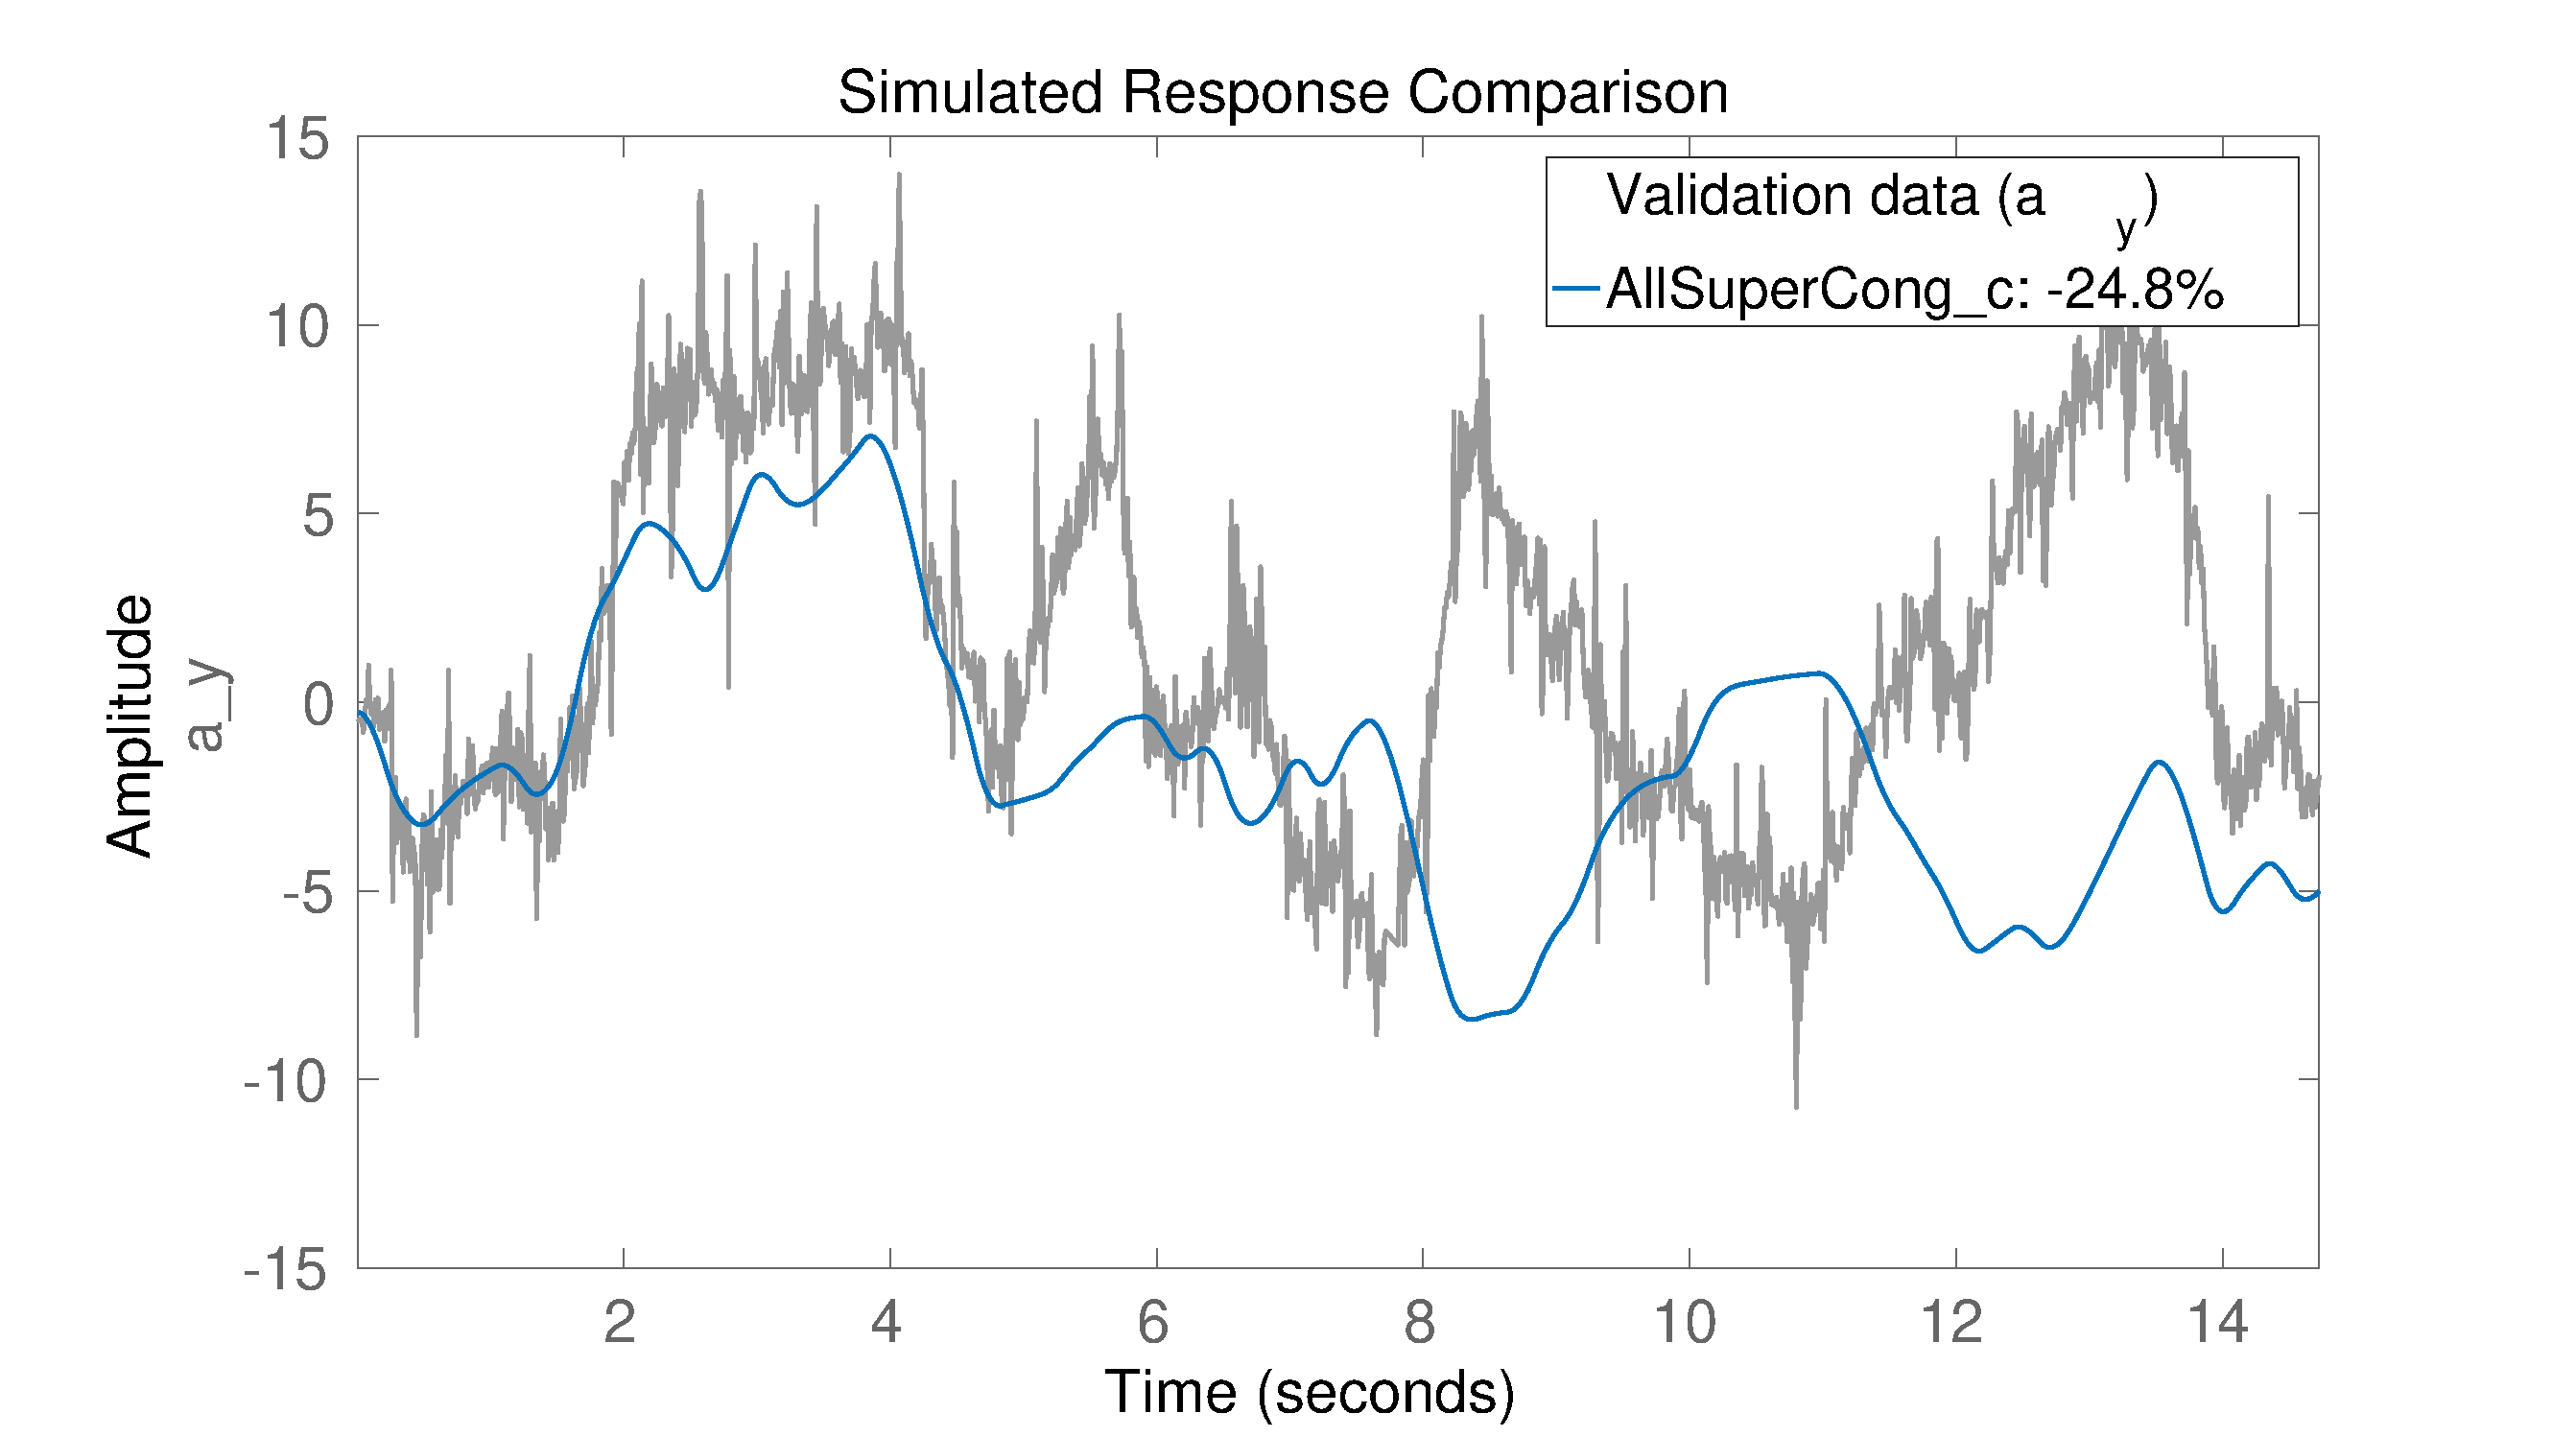
\includegraphics[width=0.4\textwidth]{linAccComparey}}
    \qquad
  \subfloat[][\label{fig:linAccComparez}Comparison of linear acceleration in the \abbrROV's z-axis between validation data and the simulated model.]{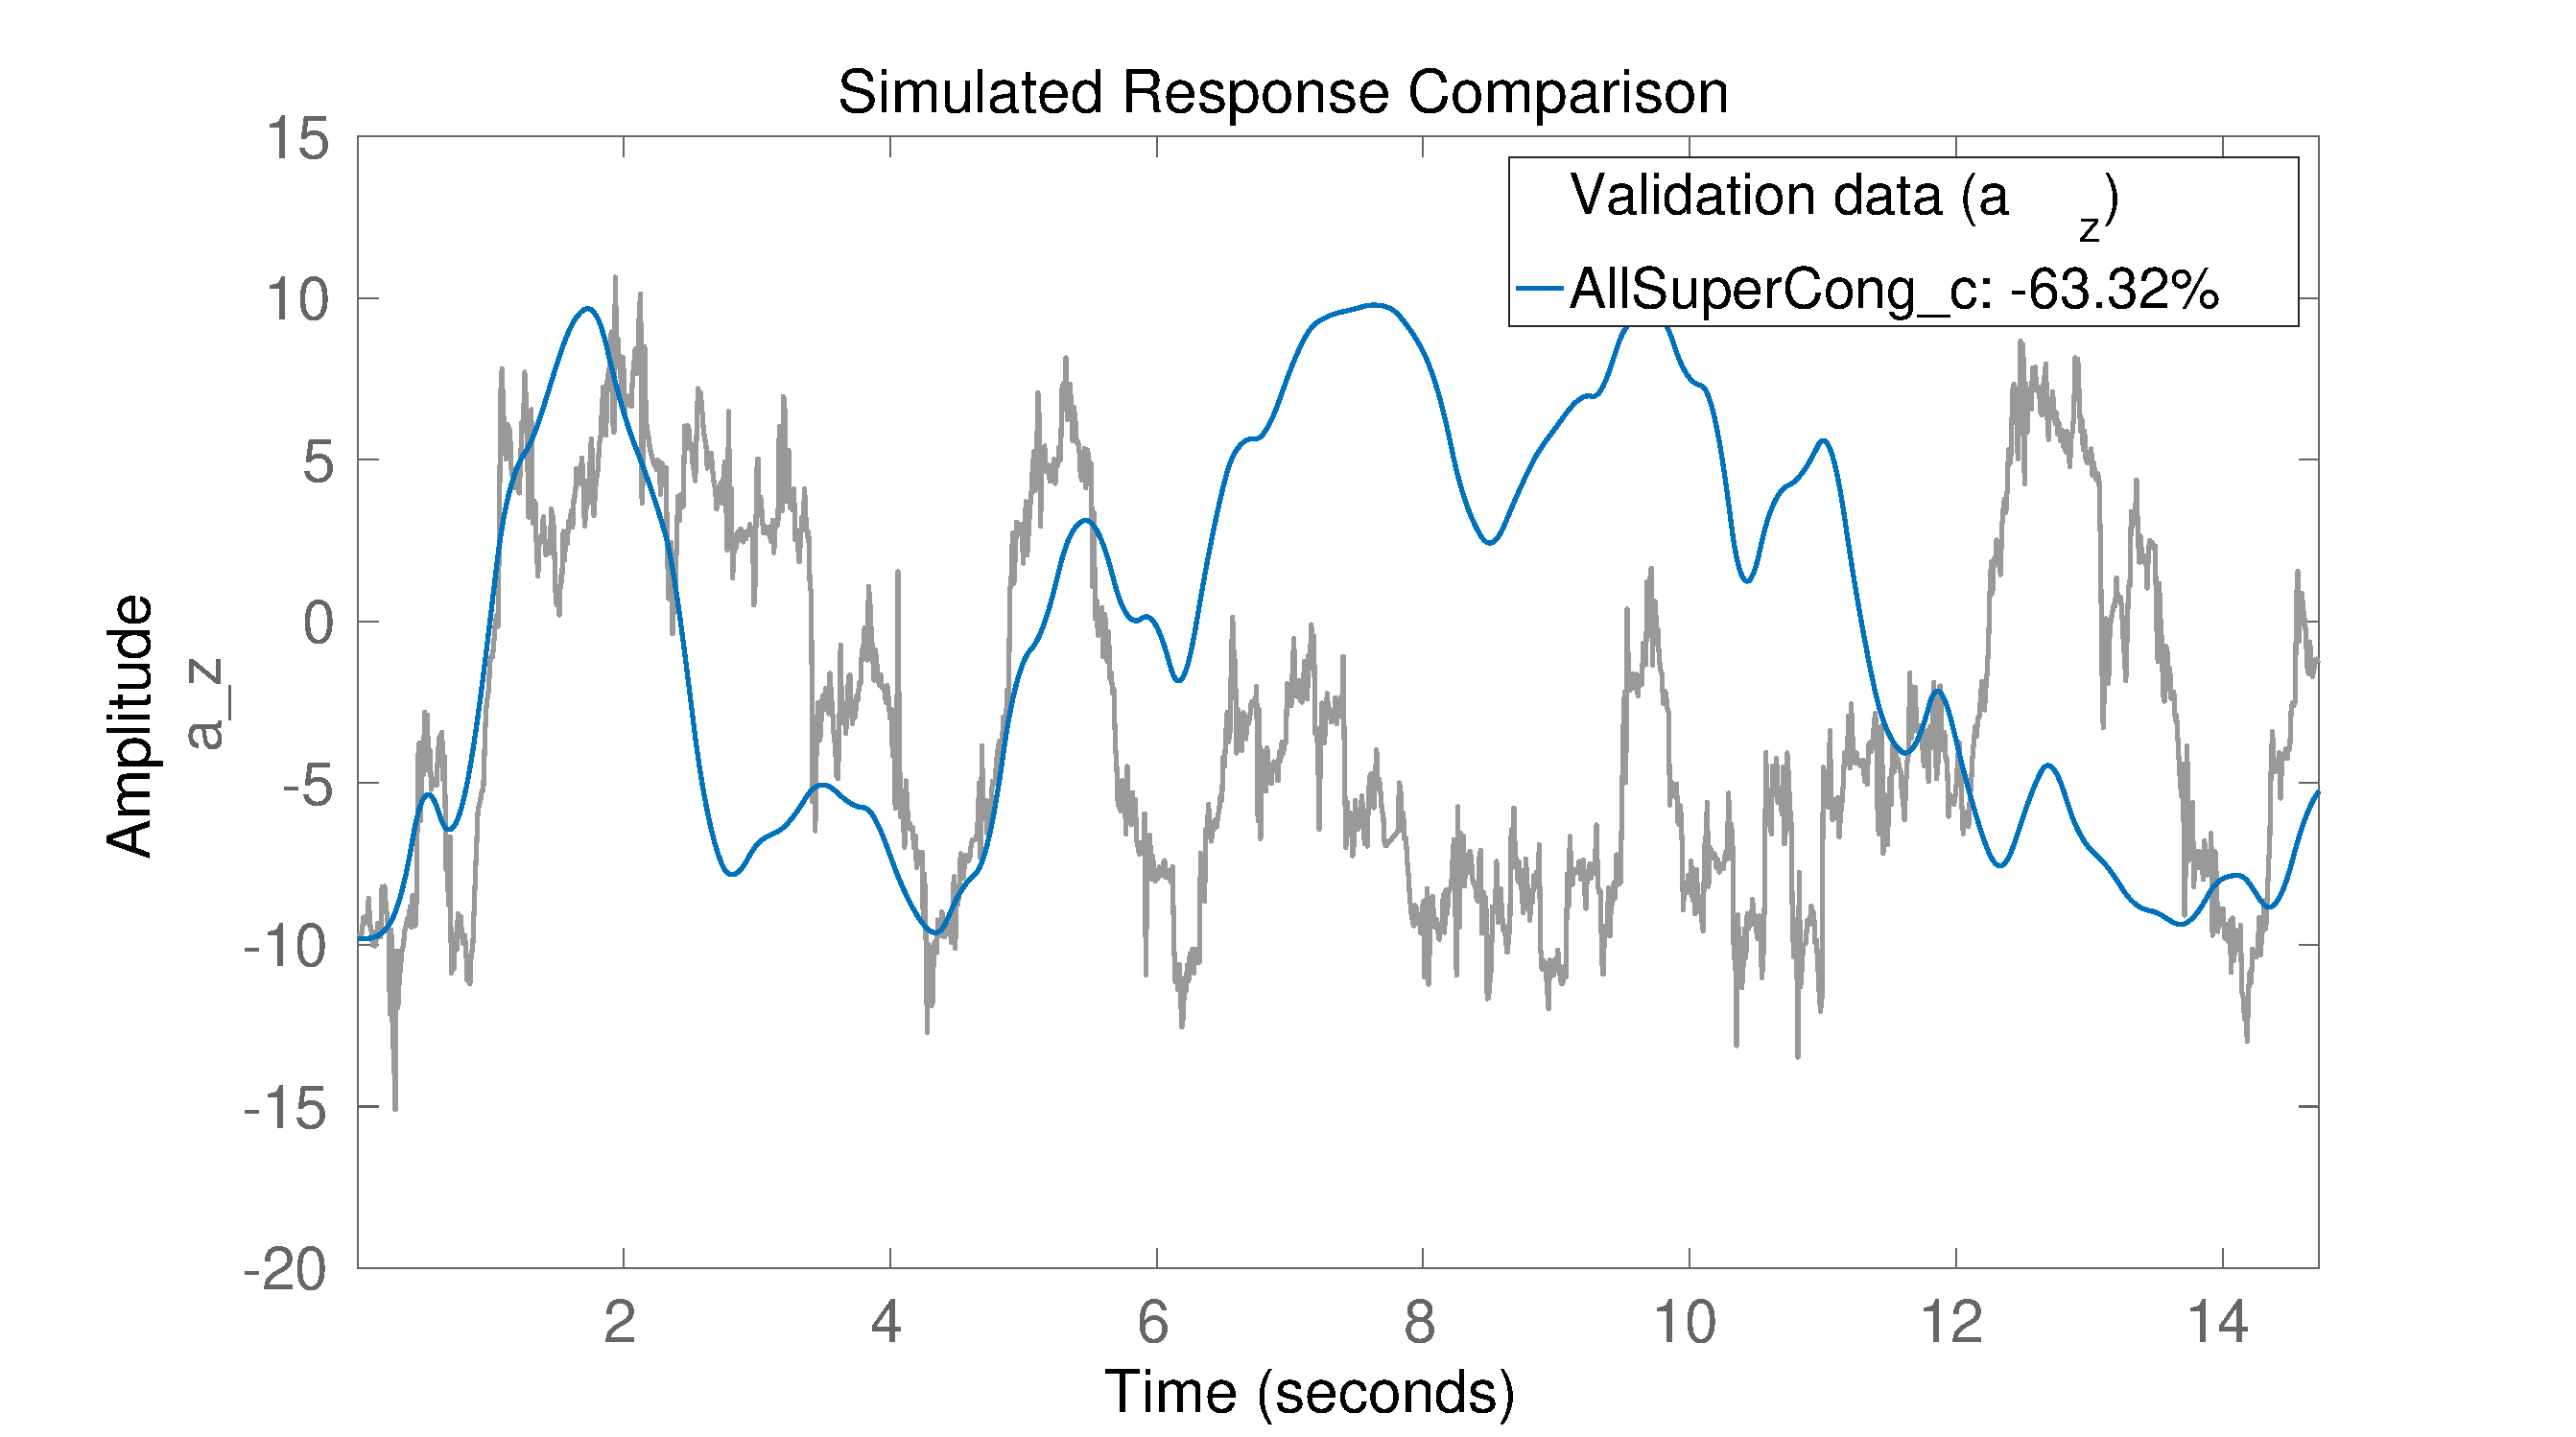
\includegraphics[width=0.4\textwidth]{linAccComparez}}
  \caption{\label{fig:angVelCompare}%
    Comparison of validation data (grey) against the simulated response from the model(blue). The fit for the model in each state is stated in each plot. During estimation was $\distance{z}{6} = 0$. The estimation used angular velocities and linear accelerations as outputs.}
\end{figure}

\begin{table}[hbp]
  \centering
  \caption{\label{tab:ResultangVellz}%
    The estimated parameters from the prediction-error method using angular velocities and linear acceleration as outputs with $\distance{z}{6} = 0.11$.}
  \begin{tabular}{l l p{0.25\linewidth}}
    \toprule%
    \textbf{Notation}  & \textbf{Starting Value} & \textbf{Estimated Value} \\
    \otoprule%   
    % Parameters that will be estimated
	$z_B$               & -0.01 	\meter 						& -0.029425  	\meter\\
    $\Kp$               & -1   	\kilogram\usk\meter\squared 	& -2.594 		\kilogram\usk\meter\squared\\
    $\Kpabsp$           & -1  	\kilogram\usk\meter\squared	& -0.30922  		\kilogram\usk\meter\squared\\
    $\Mq$               & -1  	\kilogram\usk\meter\squared	& -2.0425  		\kilogram\usk\meter\squared\\
    $\Mqabsq$           & -1  	\kilogram\usk\meter\squared	& -0.0070722  	\kilogram\usk\meter\squared\\
    $\Nr$               & -1  	\kilogram\usk\meter\squared	& -2.9364		\kilogram\usk\meter\squared\\
    $\Nrabsr$           & -1  	\kilogram\usk\meter\squared	& -2.1843 		\kilogram\usk\meter\squared\\
    $A_p$               & 1.5 	\kilogram\usk\meter\squared	&  0.7186 		\kilogram\usk\meter\squared\\
    $B_q$               & 1.5 	\kilogram\usk\meter\squared	&  0.61119		\kilogram\usk\meter\squared\\
    $C_r$               & 1.5 	\kilogram\usk\meter\squared	&  1.0981		\kilogram\usk\meter\squared\\
    \bottomrule%
  \end{tabular}
\end{table}  

\begin{figure}[tbp]
  \centering %simulation of estimation. Estimator given wrong initial state
  \subfloat[][\label{fig:angVelCompareplz6}Comparison of angular velocity around the \abbrROV's x-axis between validation data and the simulated model.]{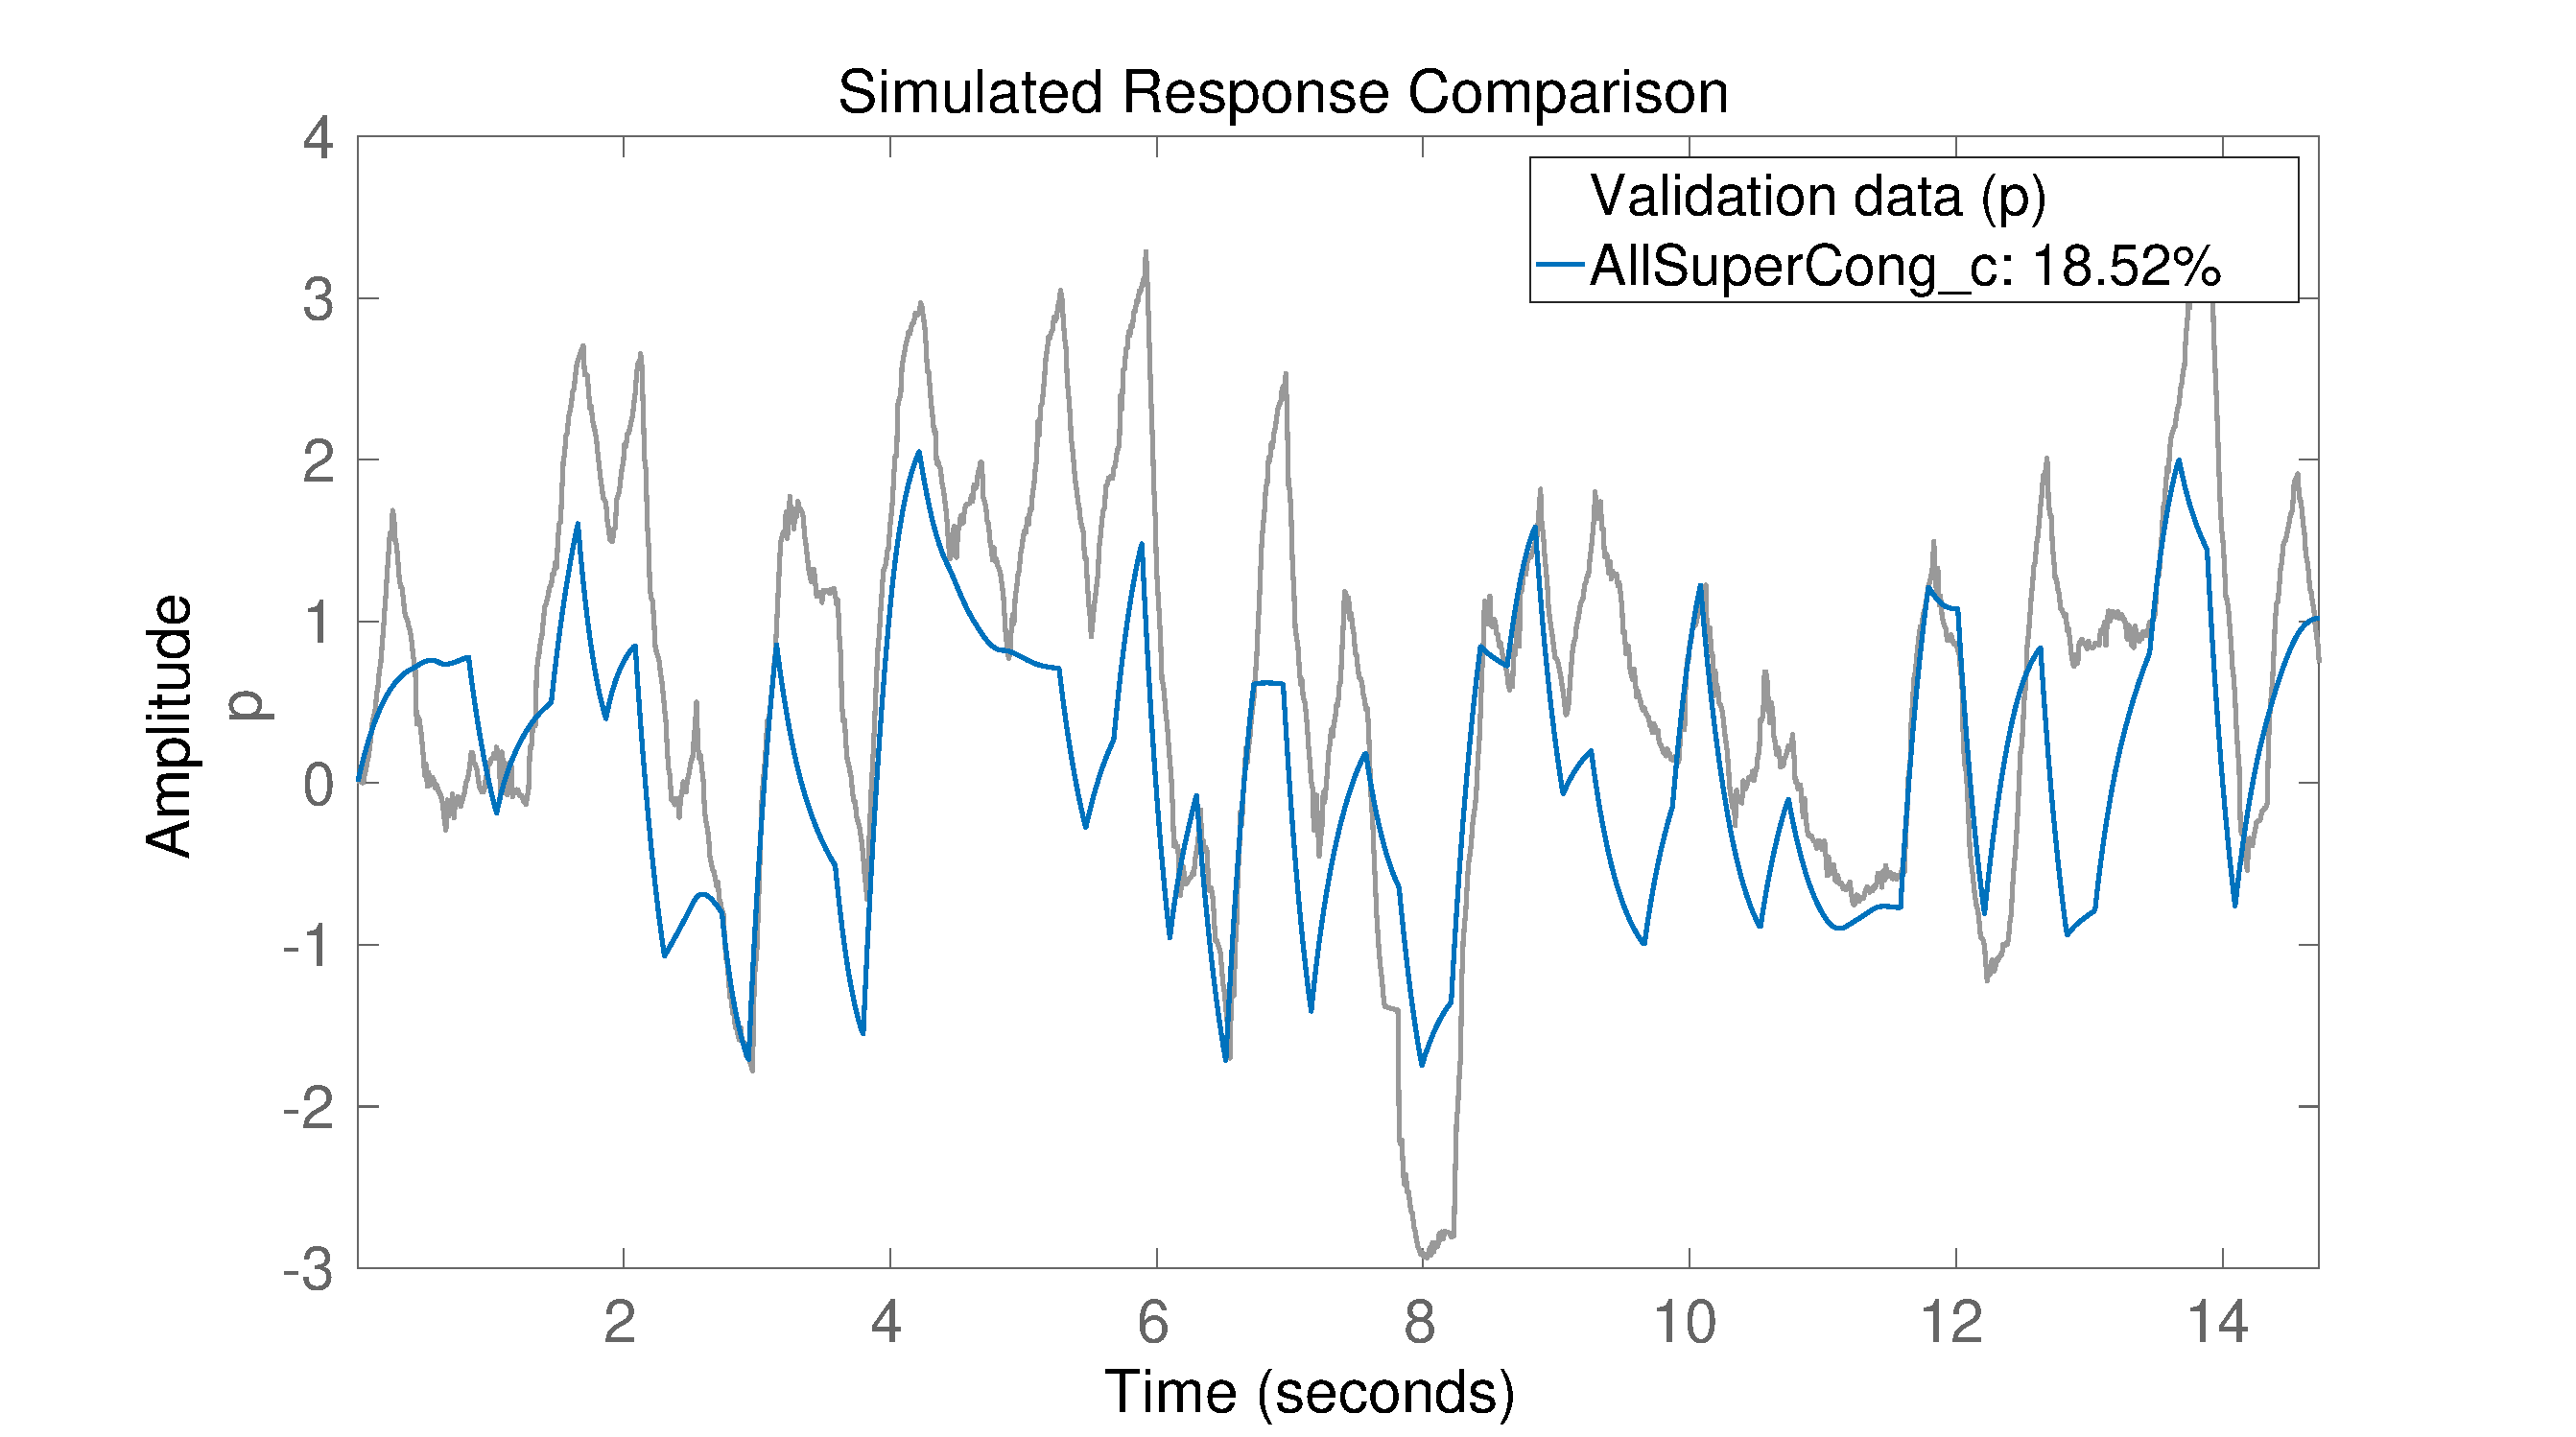
\includegraphics[width=0.4\textwidth]{angVelCompareplz6}}
  \qquad
  \subfloat[][\label{fig:angVelCompareqlz6}Comparison of angular velocity around the \abbrROV's y-axis between validation data and the simulated model.]{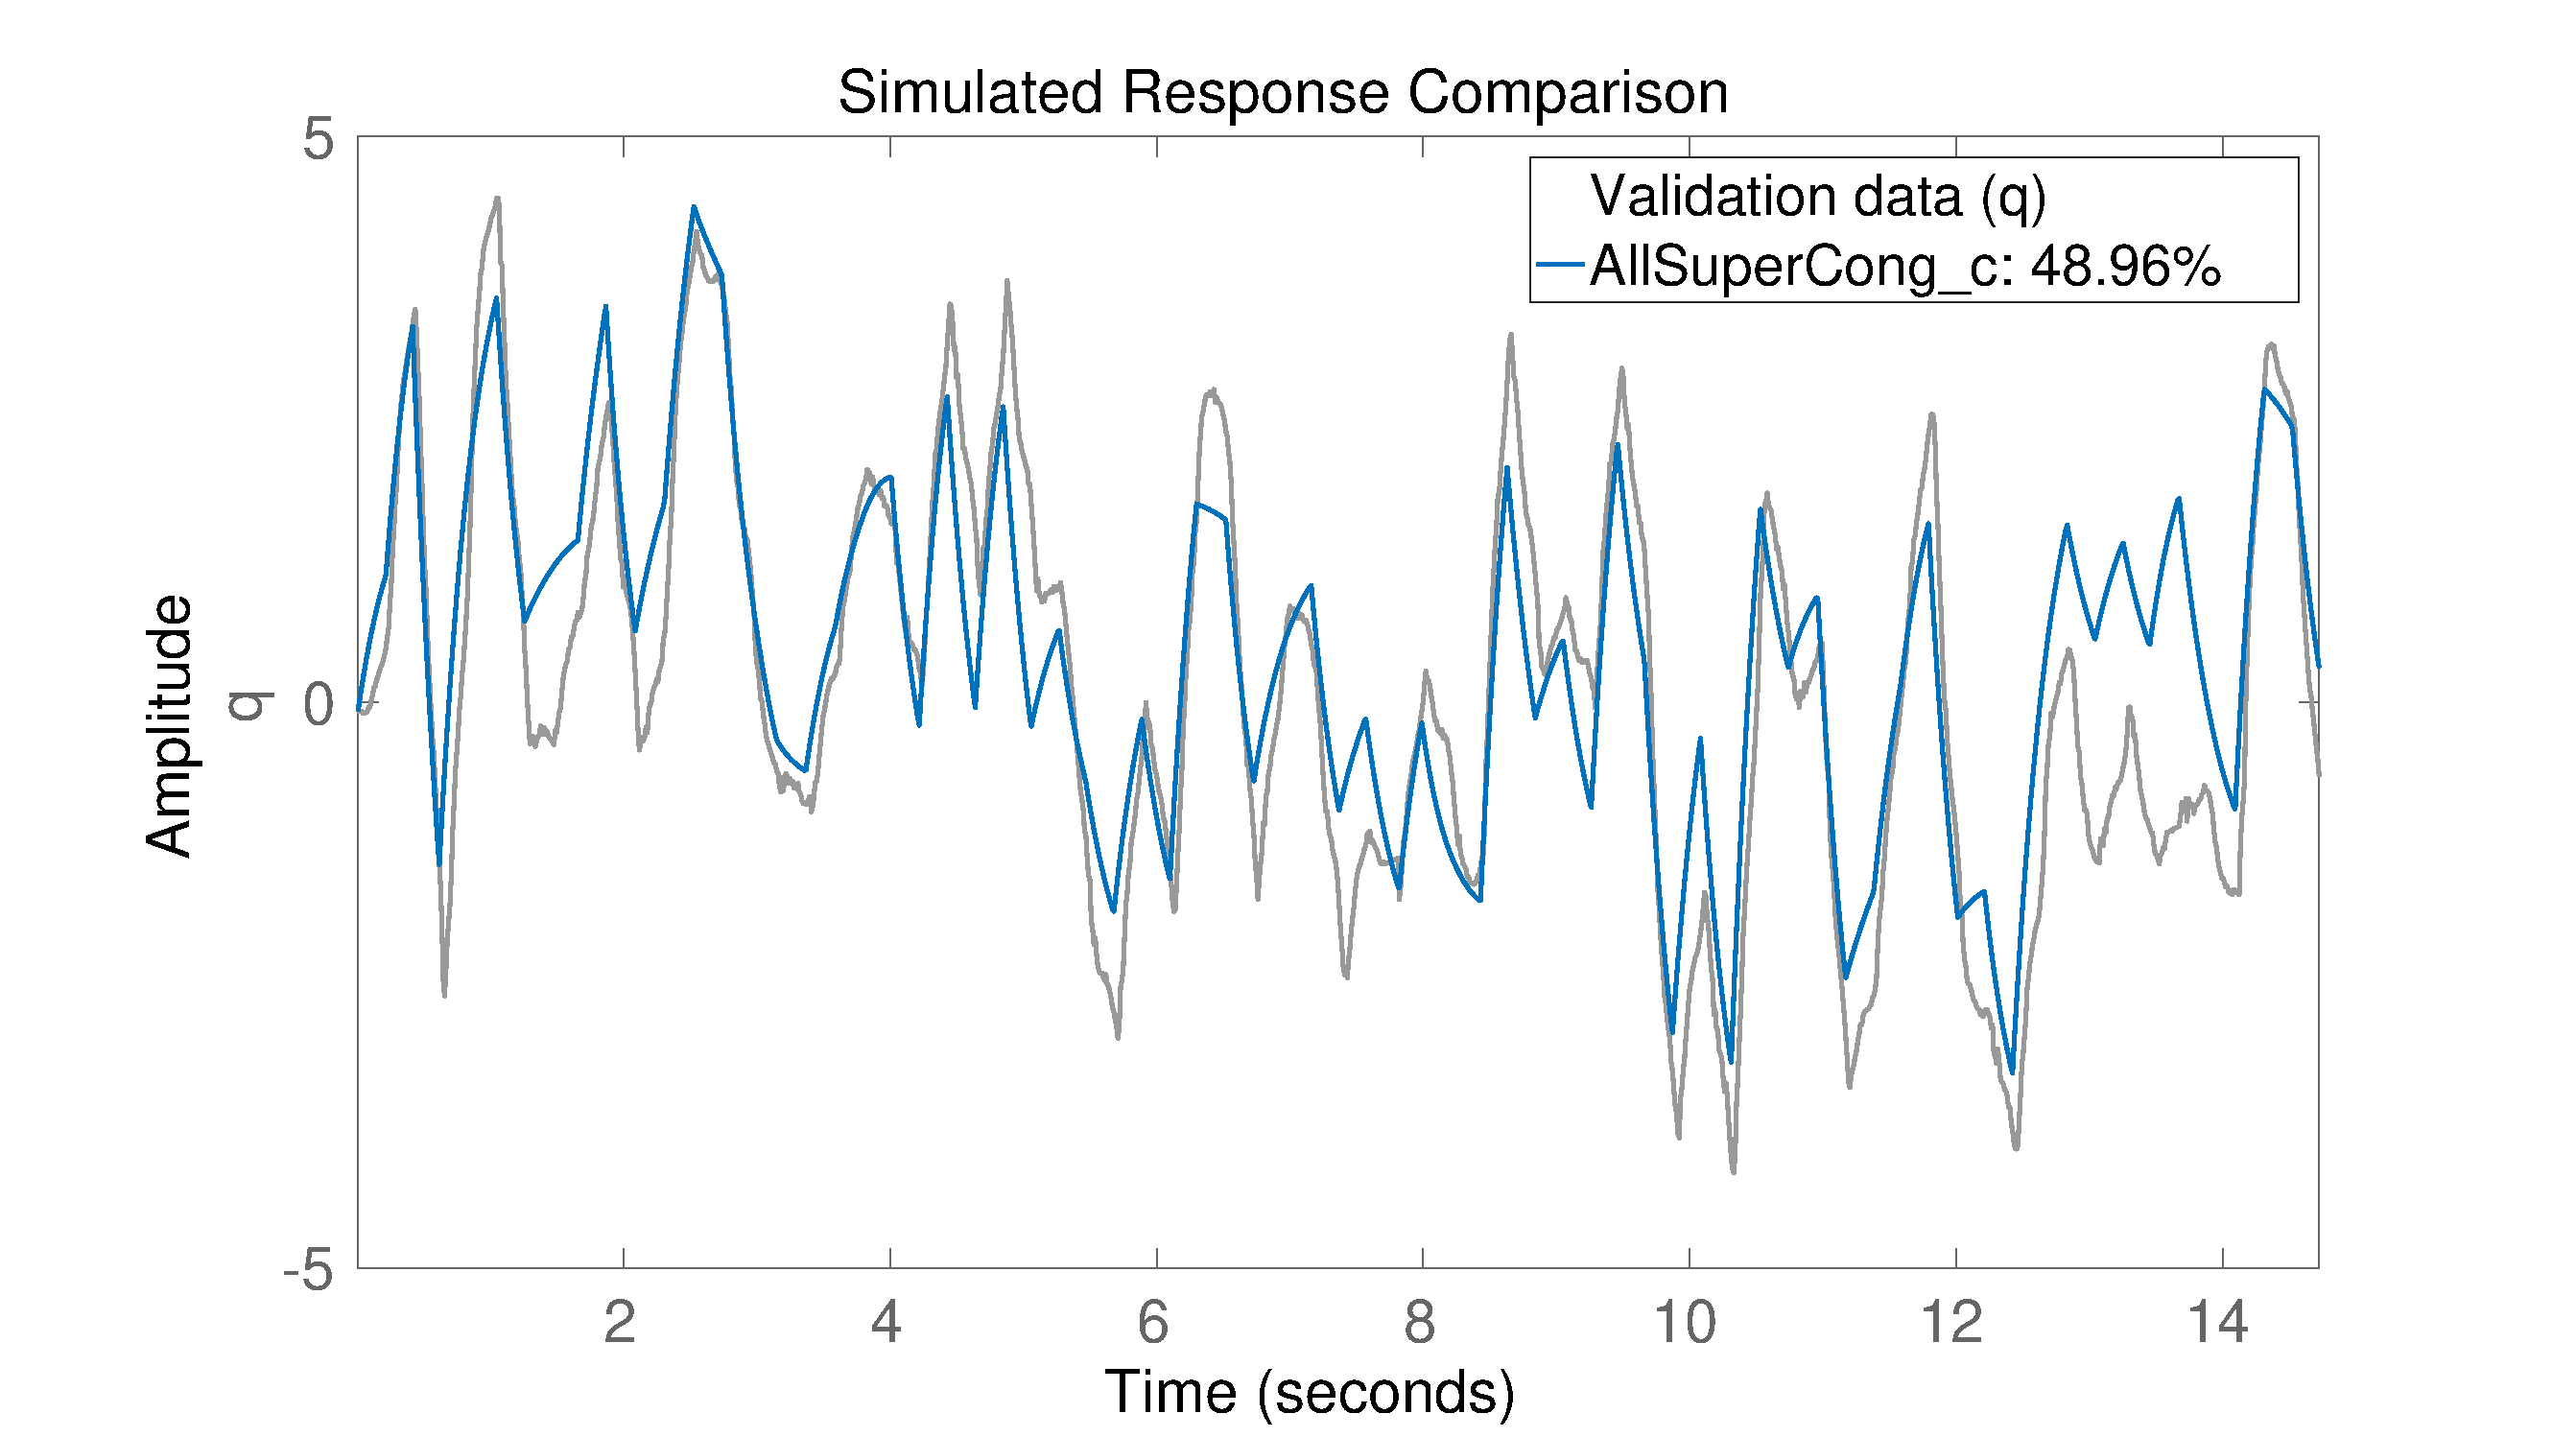
\includegraphics[width=0.4\textwidth]{angVelCompareqlz6}}
  \qquad
  \subfloat[][\label{fig:angVelComparerlz6}Comparison of angular velocity around the \abbrROV's z-axis between validation data and the simulated model.]{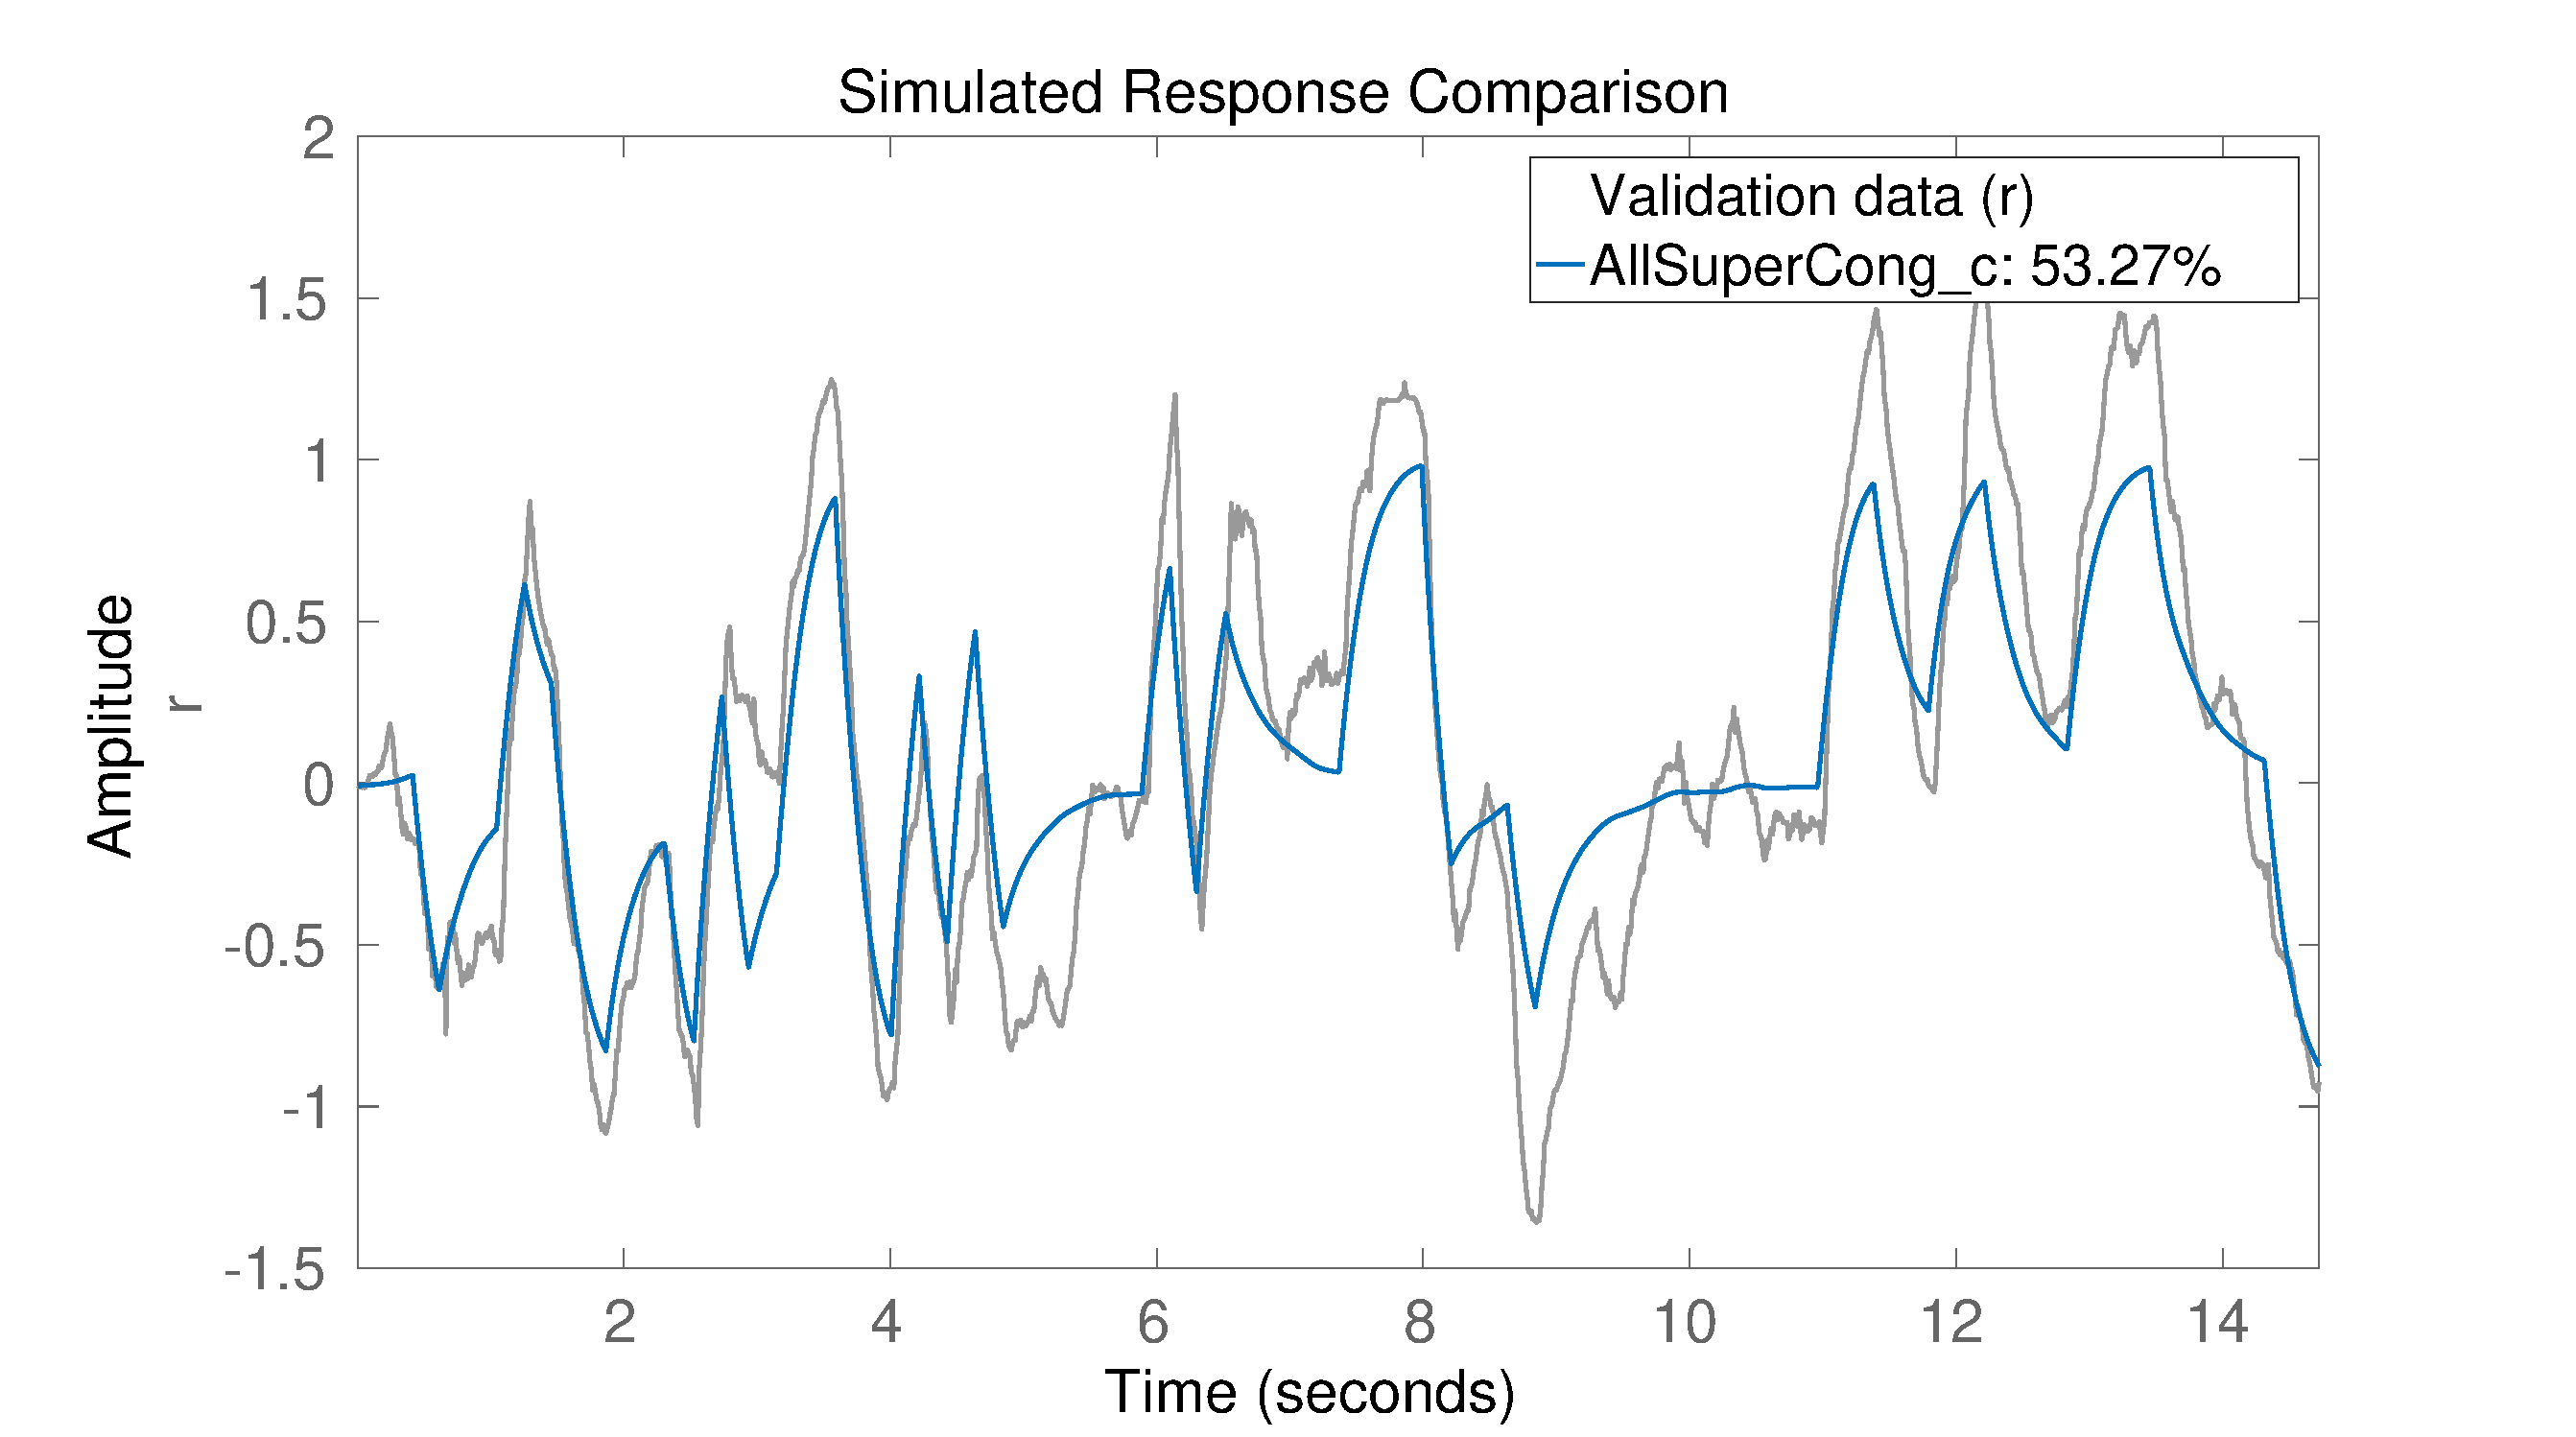
\includegraphics[width=0.4\textwidth]{angVelComparerlz6}}
    \qquad
  \subfloat[][\label{fig:linAccComparexlz6}Comparison of linear acceleration in the \abbrROV's x-axis between validation data and the simulated model.]{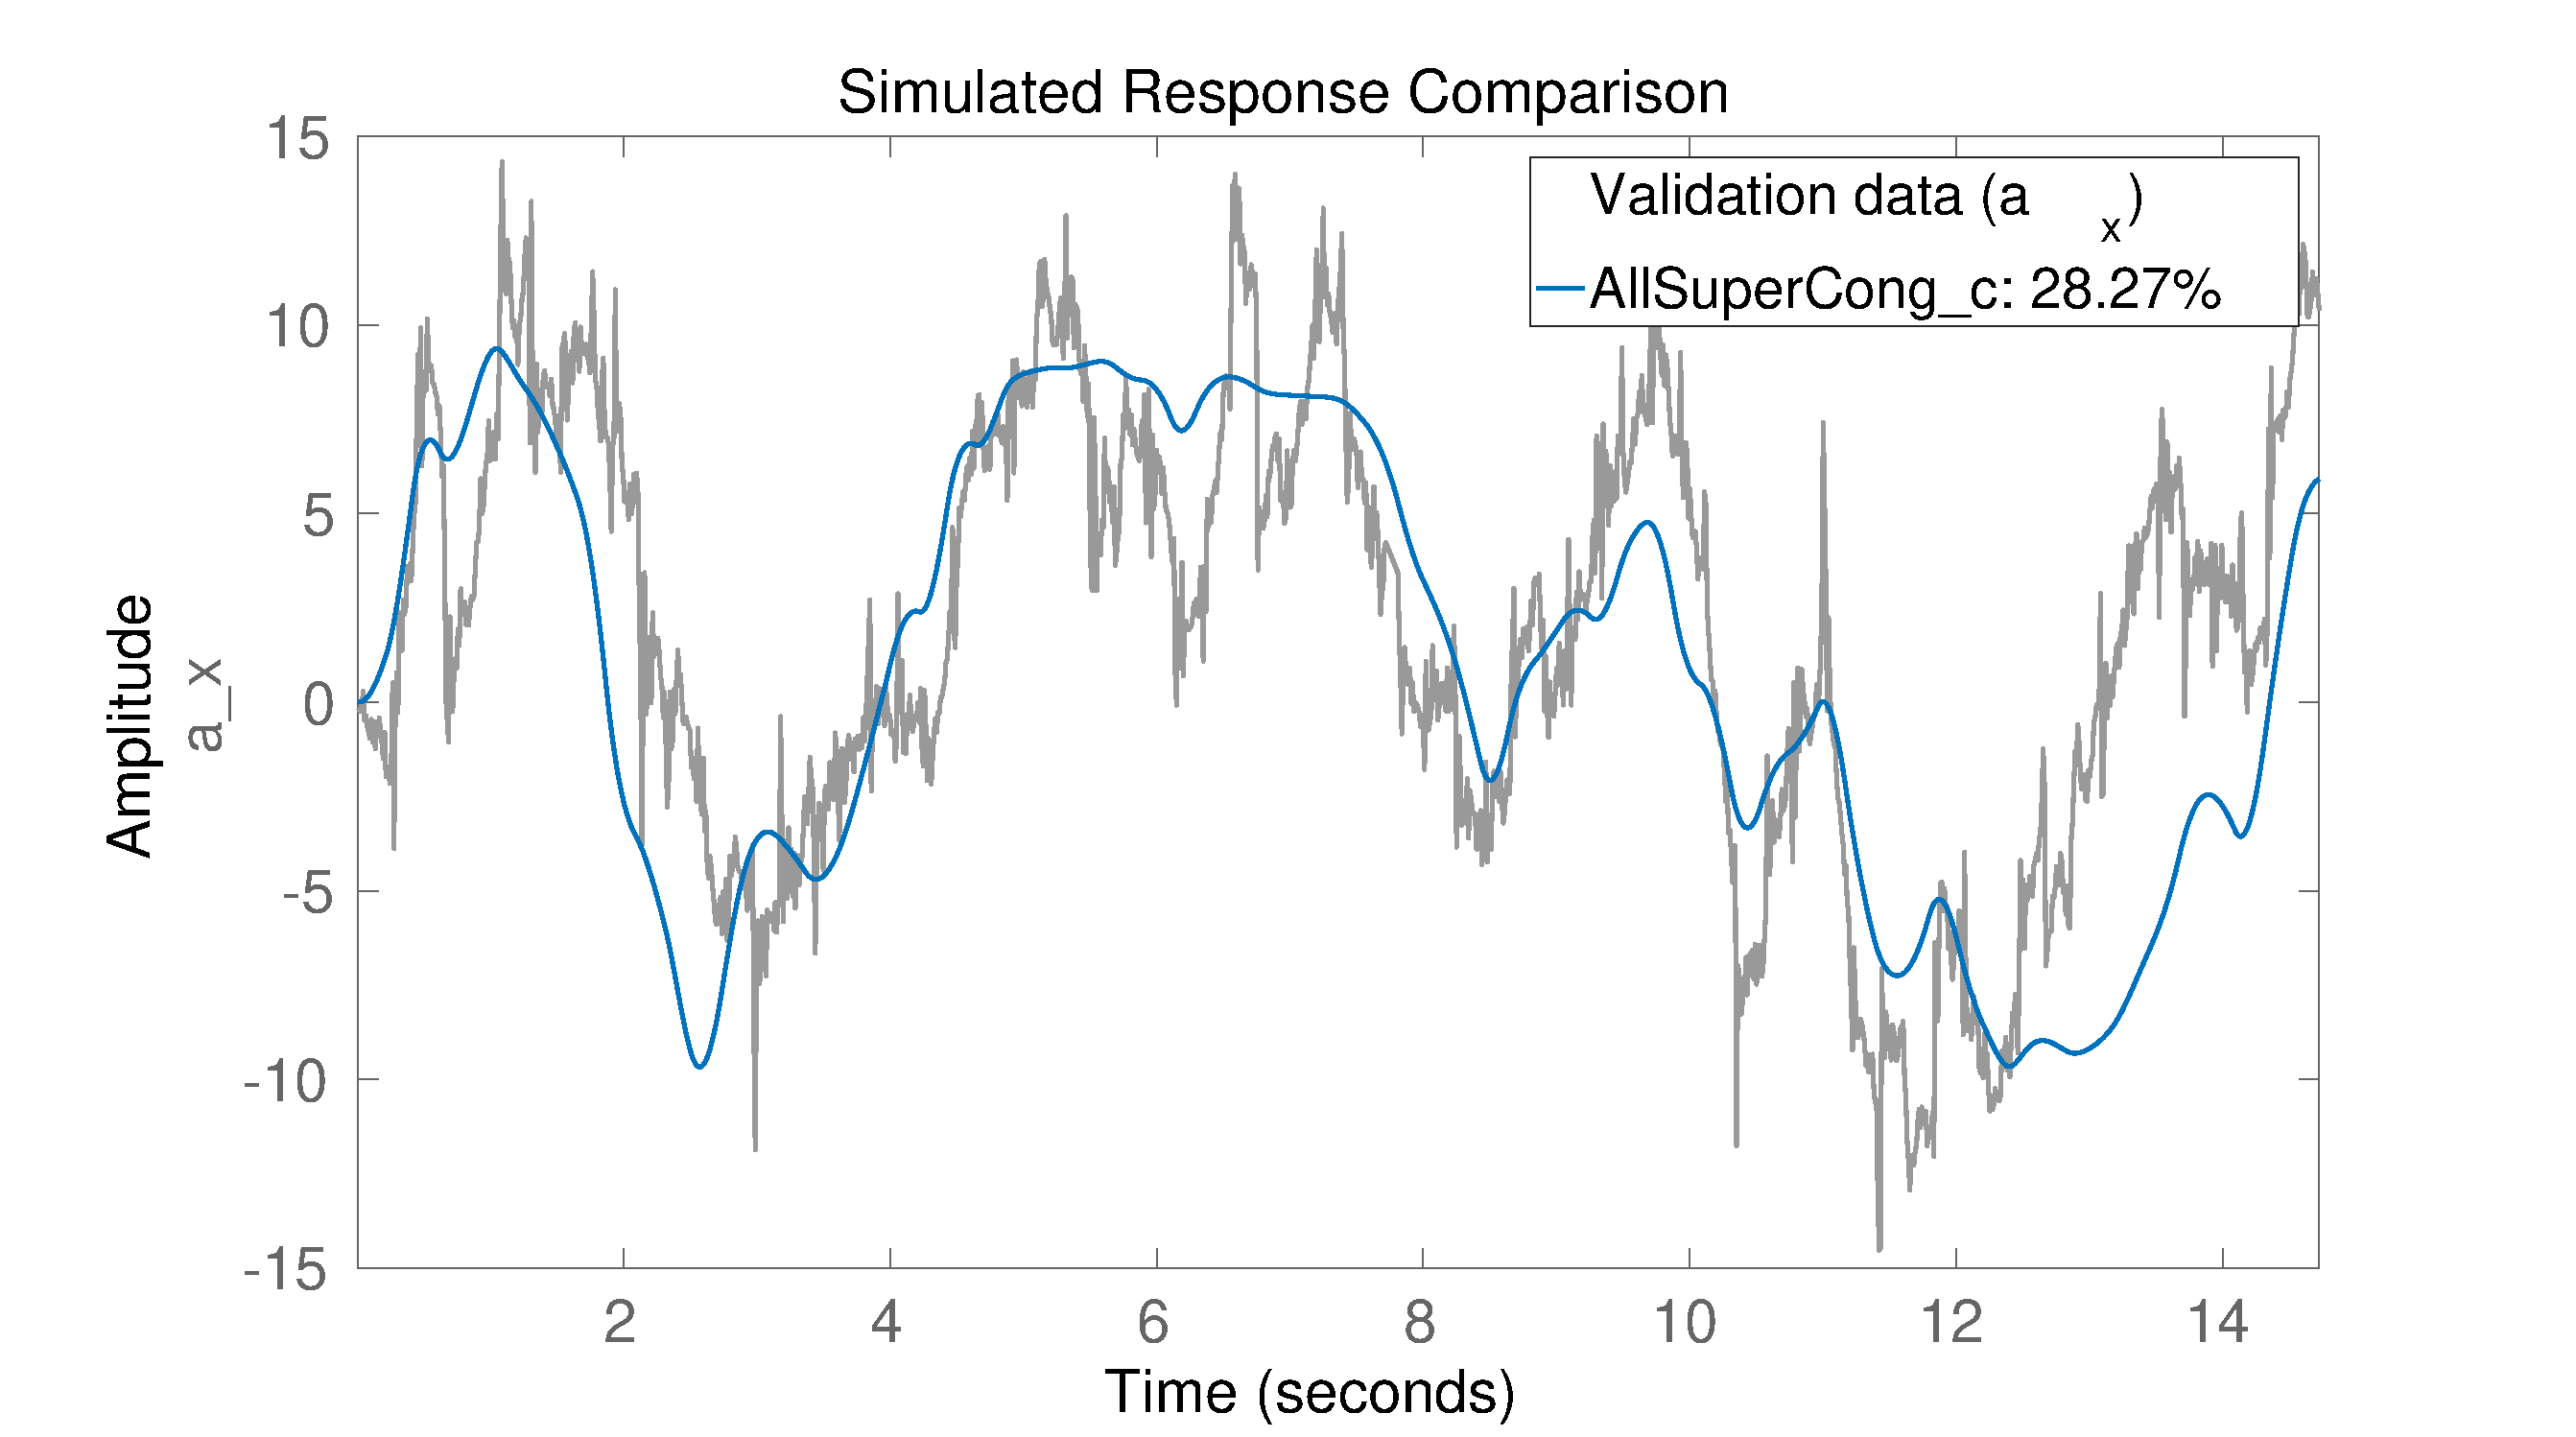
\includegraphics[width=0.4\textwidth]{linAccComparexlz6}}
    \qquad
  \subfloat[][\label{fig:linAccCompareylz6}Comparison of linear acceleration in the \abbrROV's y-axis between validation data and the simulated model.]{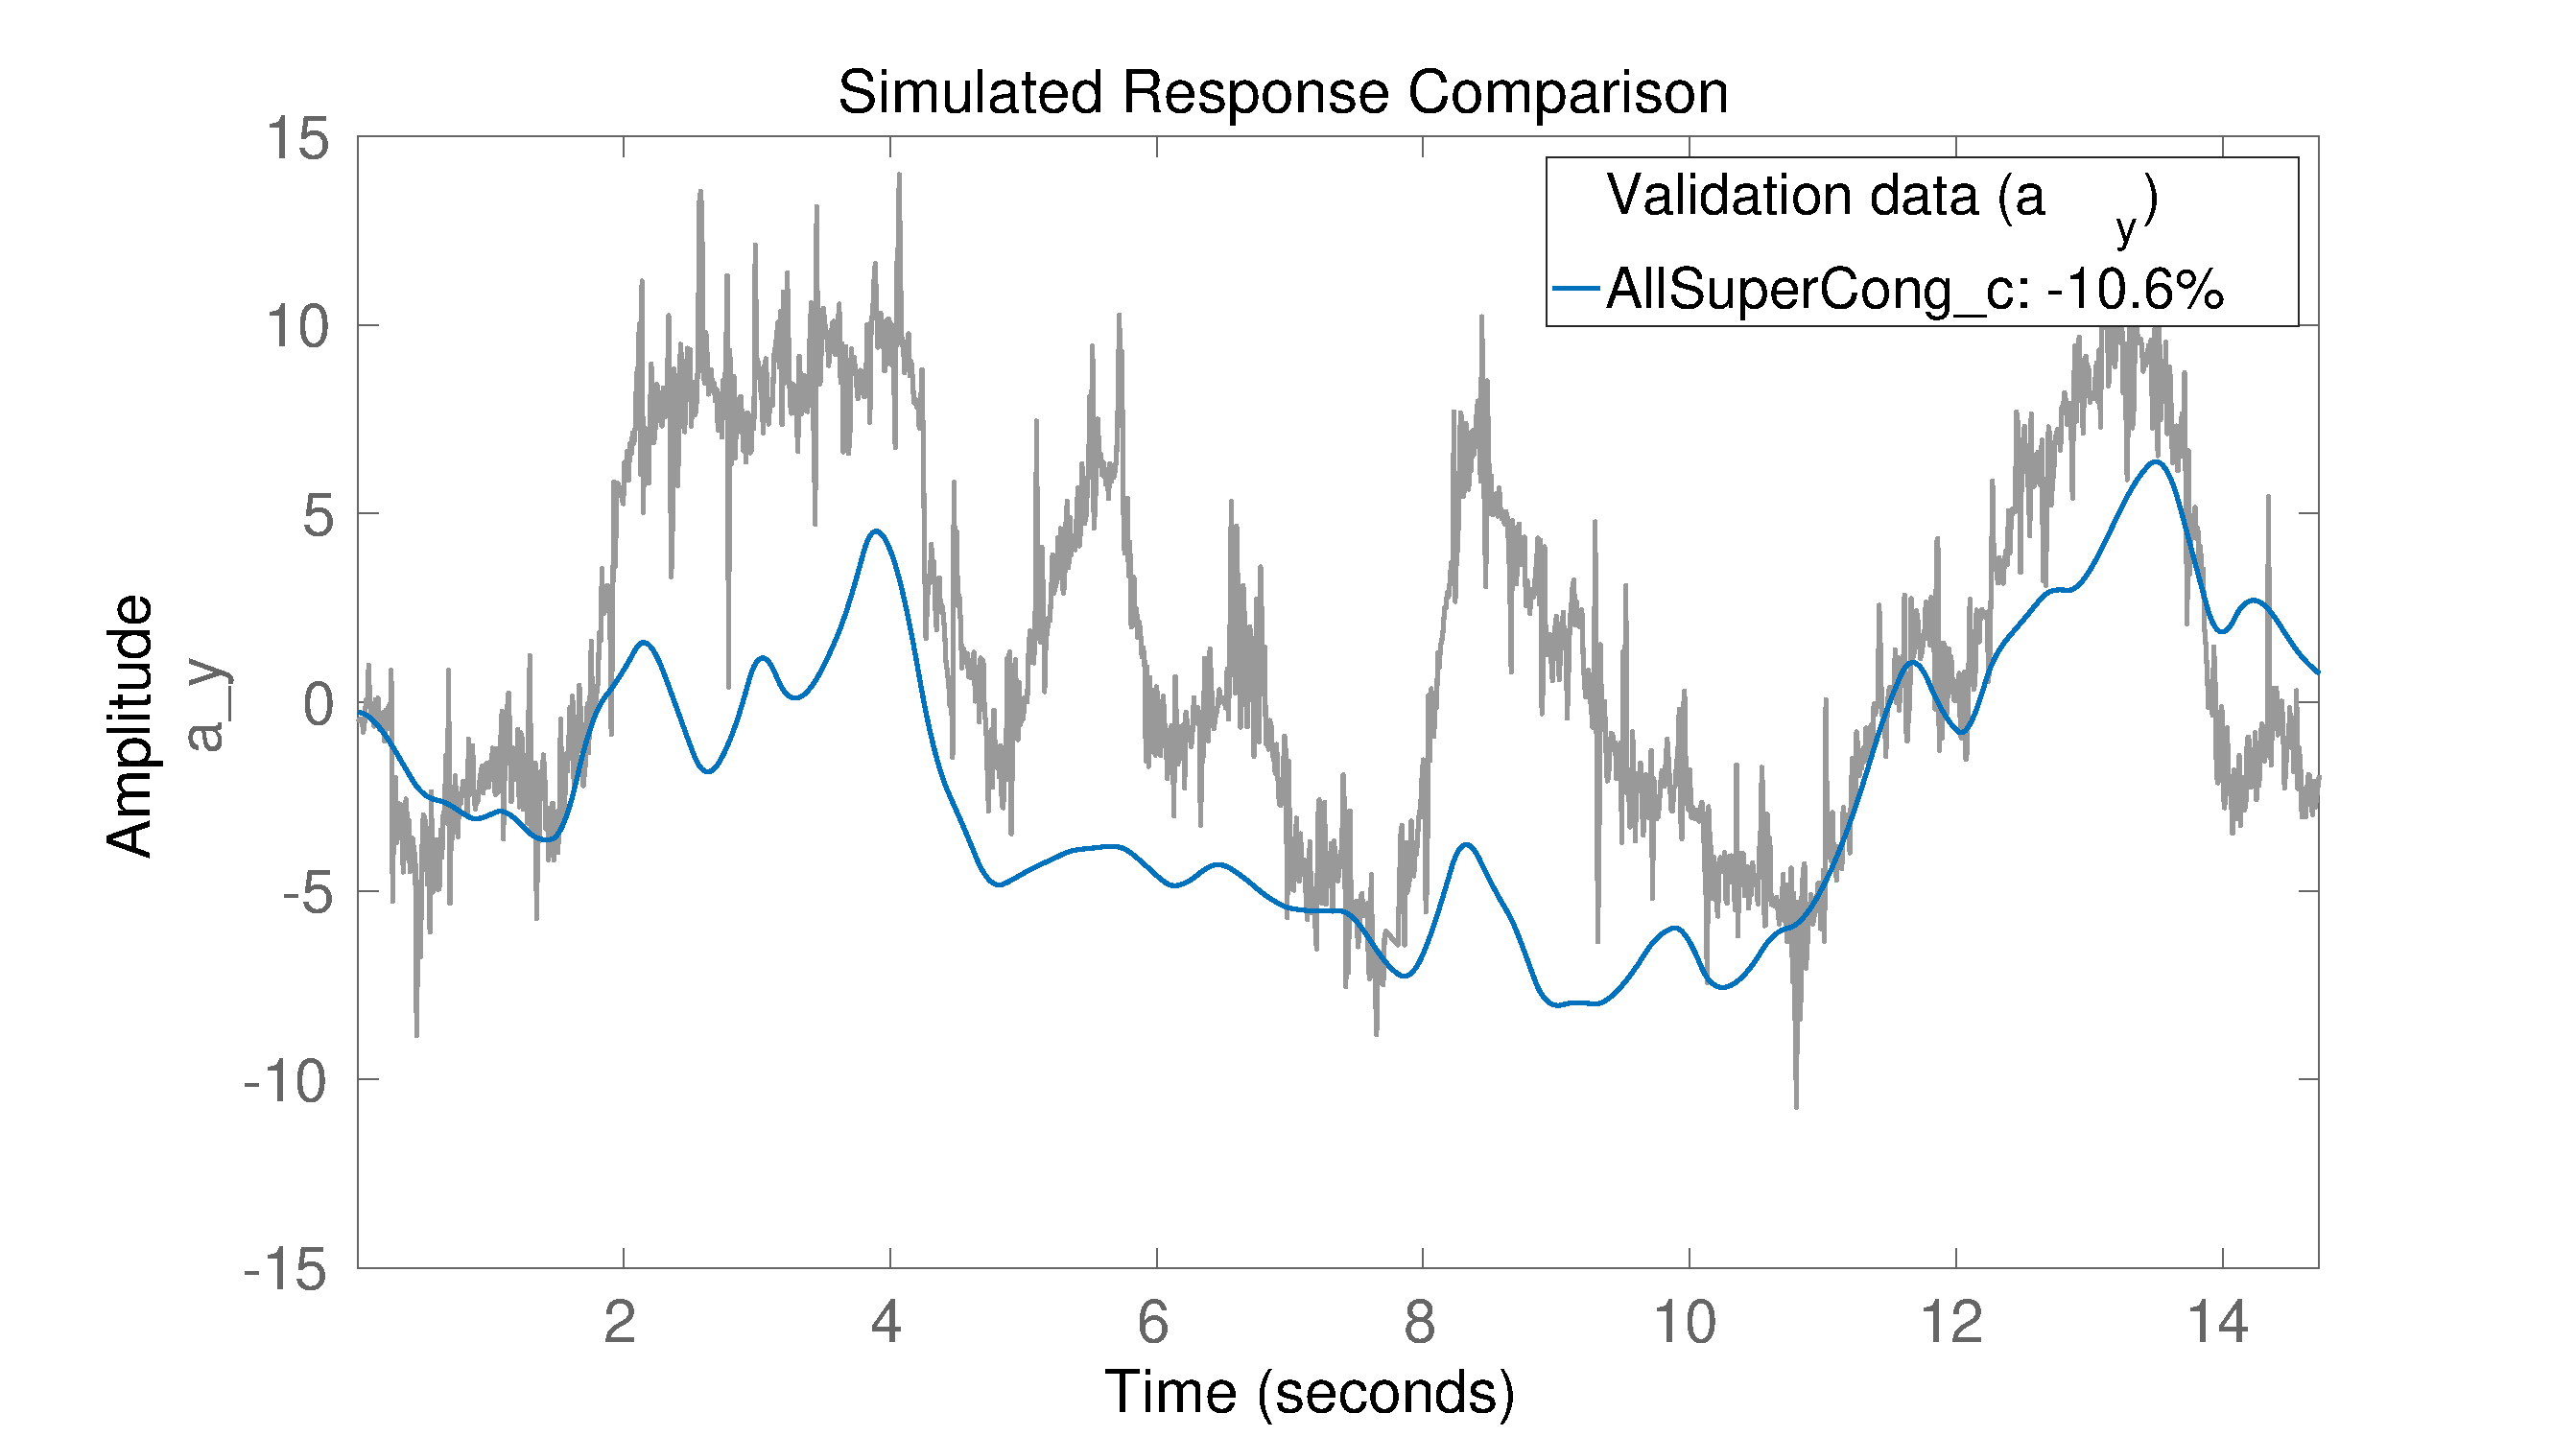
\includegraphics[width=0.4\textwidth]{linAccCompareylz6}}
    \qquad
  \subfloat[][\label{fig:linAccComparezlz6}Comparison of linear acceleration in the \abbrROV's z-axis between validation data and the simulated model.]{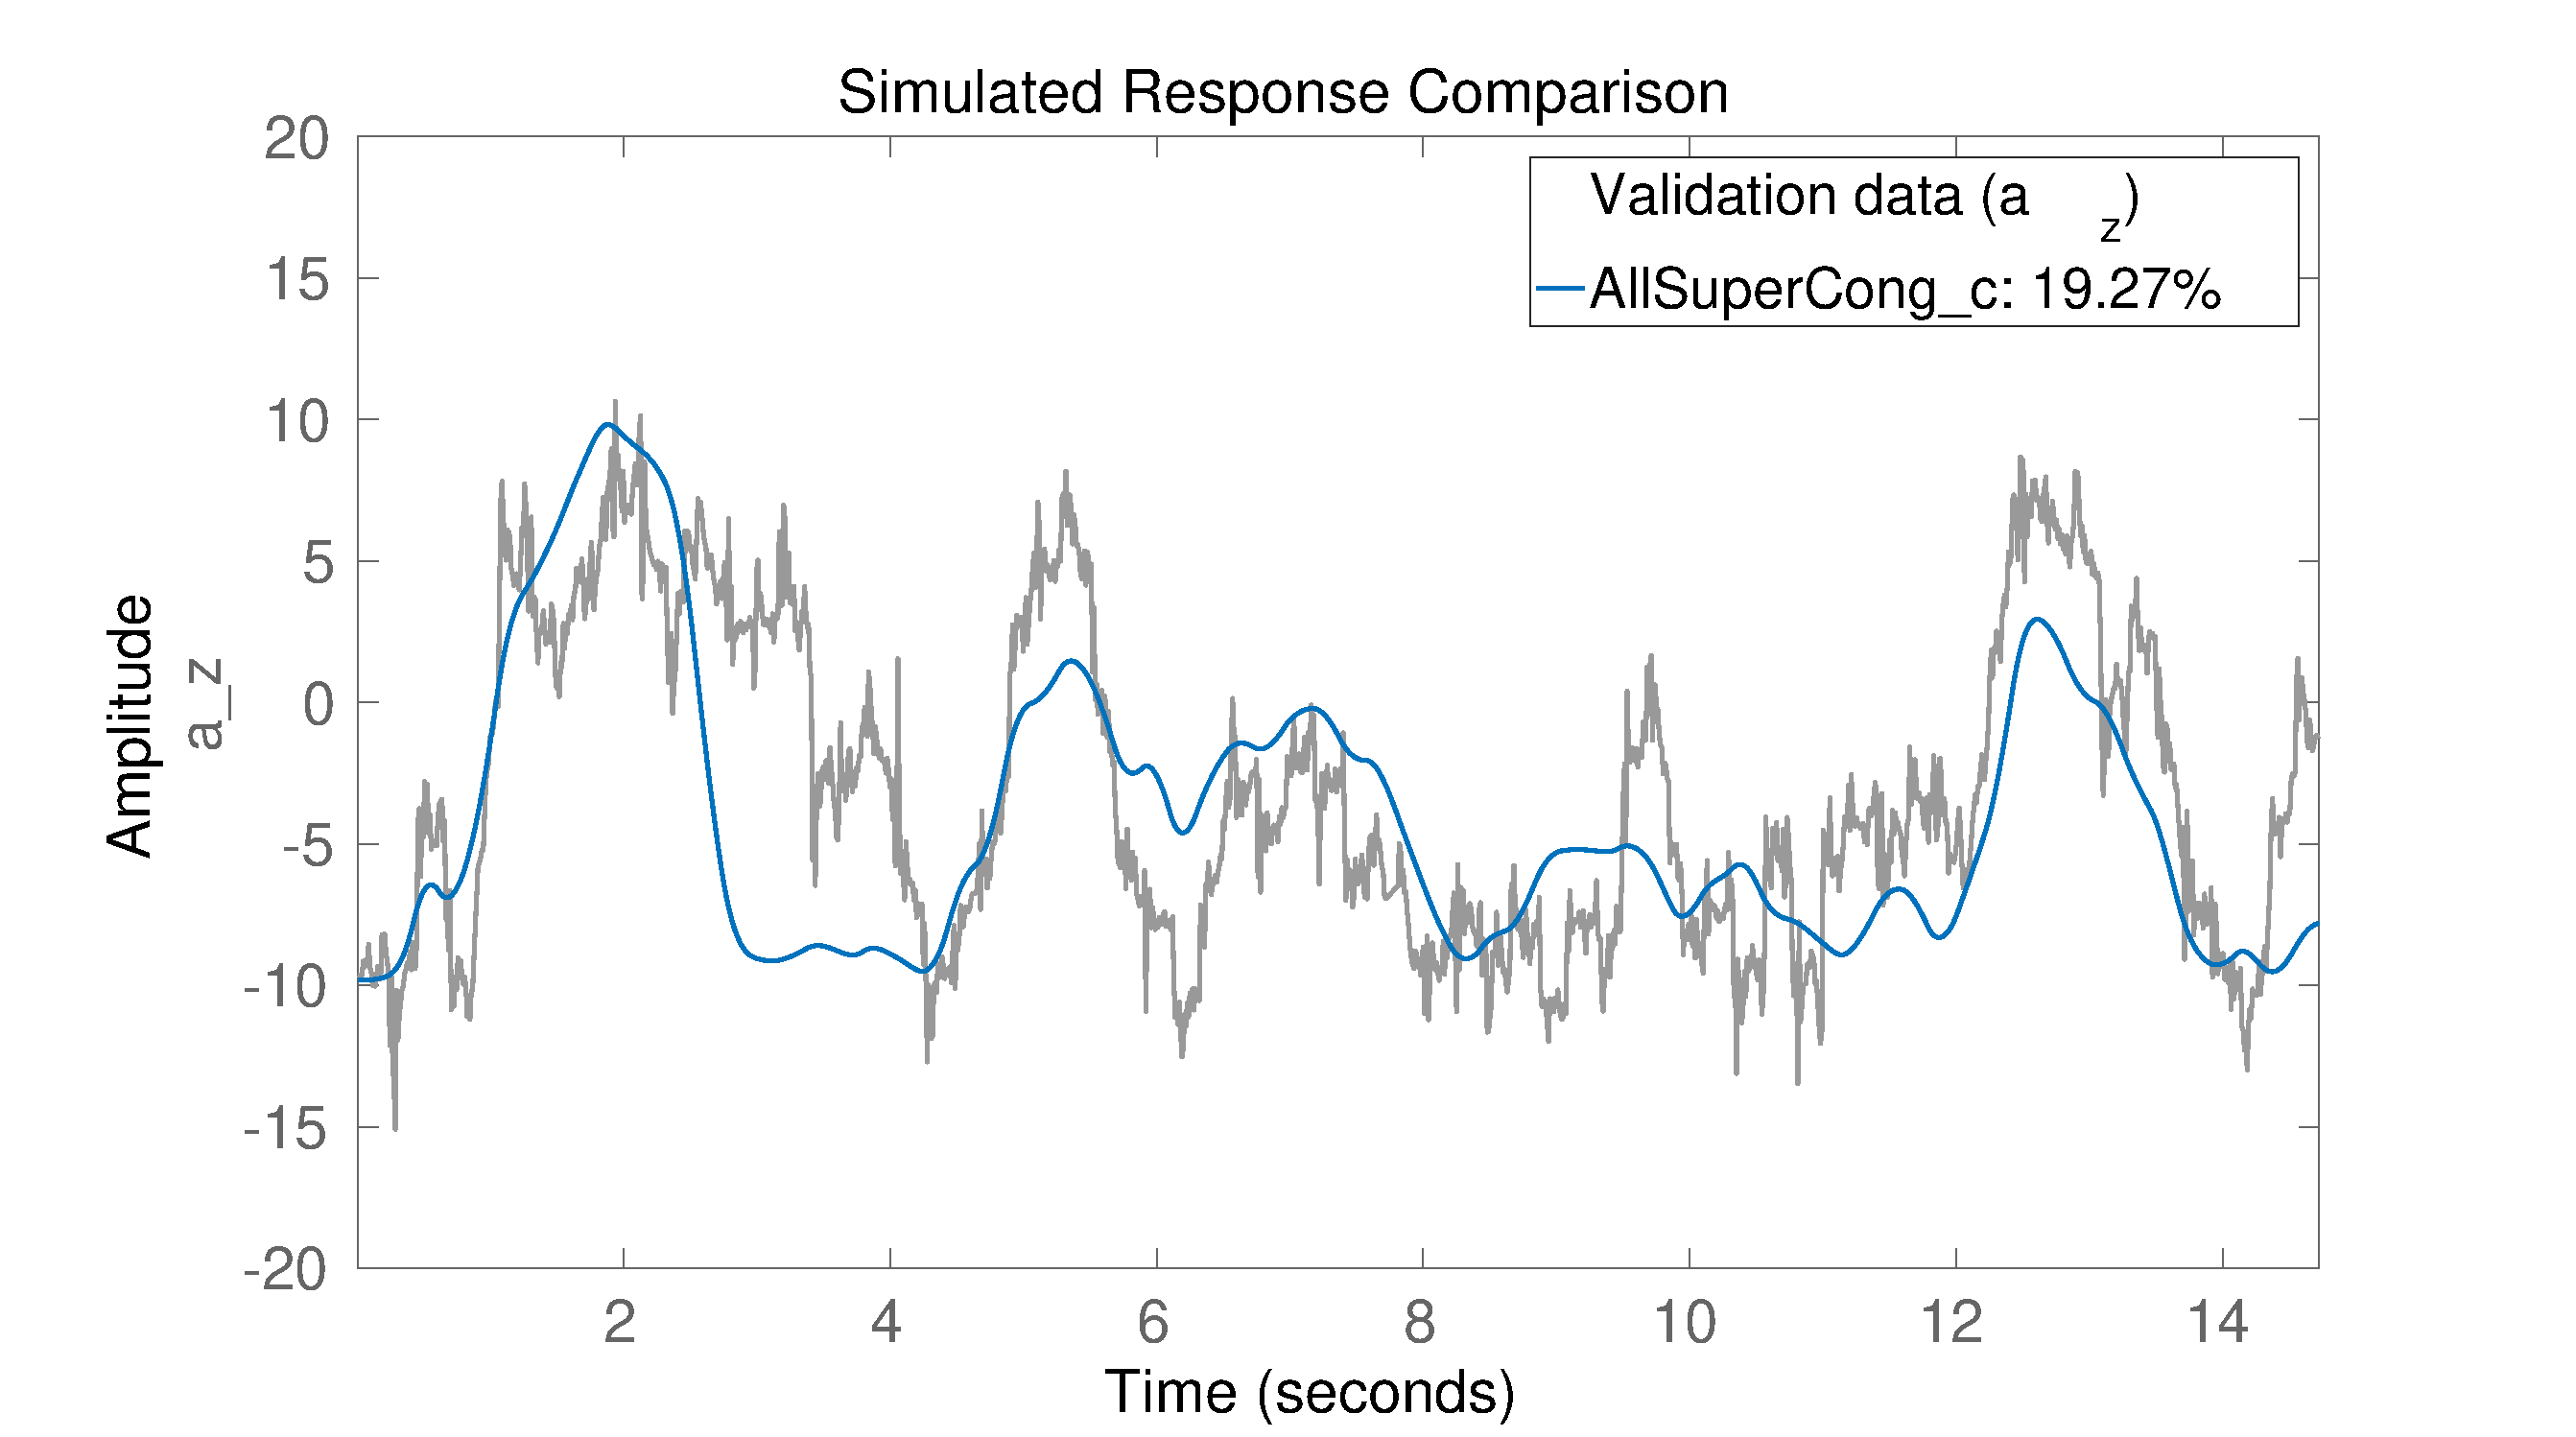
\includegraphics[width=0.4\textwidth]{linAccComparezlz6}}
  \caption{\label{fig:angVelComparelz6}%
    Comparison of validation data (grey) against the simulated response from the model(blue). The fit for the model in each state is stated in each plot. During the estimation was $\distance{z}{6} = 0.11$. The estimation used angular velocities and linear accelerations as outputs.}
\end{figure}

\subsection{Extended Kalman Filter Estimation}
Using the model defined in \sectionref{sec:KalmanEstimatorImpl} with process noise matrix
\begin{equation*}
\boldsymbol{Q}=\text{diag}[\underbrace{\overbrace{100}^{\times4}}_{\etaVector}... \underbrace{\overbrace{1000}^{\times3}}_{\nuVector}...\underbrace{\overbrace{0.01}^{\times3}}_{\boldsymbol{b}}... \underbrace{\overbrace{0.01}^{\times10}... \overbrace{0.000001}^{\times5}}_{\boldsymbol{\theta}}]\text{ ,}
\end{equation*}
measurement noise matrix
\begin{equation*}
\boldsymbol{R} = \text{diag}[\underbrace{\overbrace{0.01}^{\times3}}_{\text{Gyro}}... \underbrace{\overbrace{0.1}^{\times3}}_{\text{Acc}}... \underbrace{\overbrace{100}^{\times3}}_{\text{mag}}]
\end{equation*}
The extremely low values of the last five elements in $\boldsymbol{Q}$ were chosen to fixate the measured moment arms of the thrusters. Four data sets were feed in to the estimator and a fifth was used as validation data. All data sets were of excitations in $p$, $q$ and $r$. Parameter values from the estimation can be viewed together with the starting state in \tableref{tab:ResultKalmanFixedMomentArms}.
\begin{table}[hbp]
  \centering
  \caption{\label{tab:ResultKalmanFixedMomentArms}%
    The estimated parameters from the Kalman estimator method. Moment arms are fixed to measured values.}
  \begin{tabular}{l l p{0.25\linewidth}}
    \toprule%
    \textbf{Notation}  & \textbf{Starting Value} & \textbf{Estimated Value} \\
    \otoprule%   
    % Parameters that will be estimated
    $\etaVector$			&$[1\ 0\ 0\ 0]^T$					&\\
    $\nuVector$			&$[0\ 0\ 0]^T$						&\\
    $\boldsymbol{b}$		&$[0\ 0\ 0]^T$						&\\
	$z_B$               & -0.05 	\meter 						& -0.0606  	\meter\\
    $\Kp$               & -1   	\kilogram\usk\meter\squared 	& -0.8745 		\kilogram\usk\meter\squared\\
    $\Kpabsp$           & -1  	\kilogram\usk\meter\squared	& -0.6279  		\kilogram\usk\meter\squared\\
    $\Mq$               & -1  	\kilogram\usk\meter\squared	& -0.8529  		\kilogram\usk\meter\squared\\
    $\Mqabsq$           & -1  	\kilogram\usk\meter\squared	& -0.2505  	\kilogram\usk\meter\squared\\
    $\Nr$               & -1  	\kilogram\usk\meter\squared	& -1.0469		\kilogram\usk\meter\squared\\
    $\Nrabsr$           & -1  	\kilogram\usk\meter\squared	& -1.0405 		\kilogram\usk\meter\squared\\
    $A_p$               & 1 	\kilogram\usk\meter\squared	&  0.9728 		\kilogram\usk\meter\squared\\
    $B_q$               & 1 	\kilogram\usk\meter\squared	&  0.7266		\kilogram\usk\meter\squared\\
    $C_r$               & 1 	\kilogram\usk\meter\squared	&  1.2013		\kilogram\usk\meter\squared\\
    $\distance{x}{1}$  &0.19 \meter & 0.1900 \meter\\
    $\distance{y}{1}$  &0.11 \meter & 0.1106 \meter\\
    $\distance{x}{2}$  &0.19 \meter & 0.1900 \meter\\
    $\distance{y}{2}$  &0.11 \meter & 0.1106 \meter\\
    $\distance{y}{3}$  &0.11 \meter & 0.1099 \meter\\
    $\distance{x}{5}$  &0.17 \meter & 0.1704 \meter\\
    $\distance{y}{4}$  &0.11 \meter & 0.1099 \meter\\
    $\distance{z}{6}$  &0.11 \meter & 0.1091 \meter\\ 
    \bottomrule%
  \end{tabular}
\end{table}
The fit of the model using the estimated parameters can be viewed in \figureref{fig:ResultKalmanFixedMomentArms}
% results kalman fixed moment arms
\begin{figure}[tbp]
  \centering
  \subfloat[][Comparison between a simulated model response and validation data in $p$.]{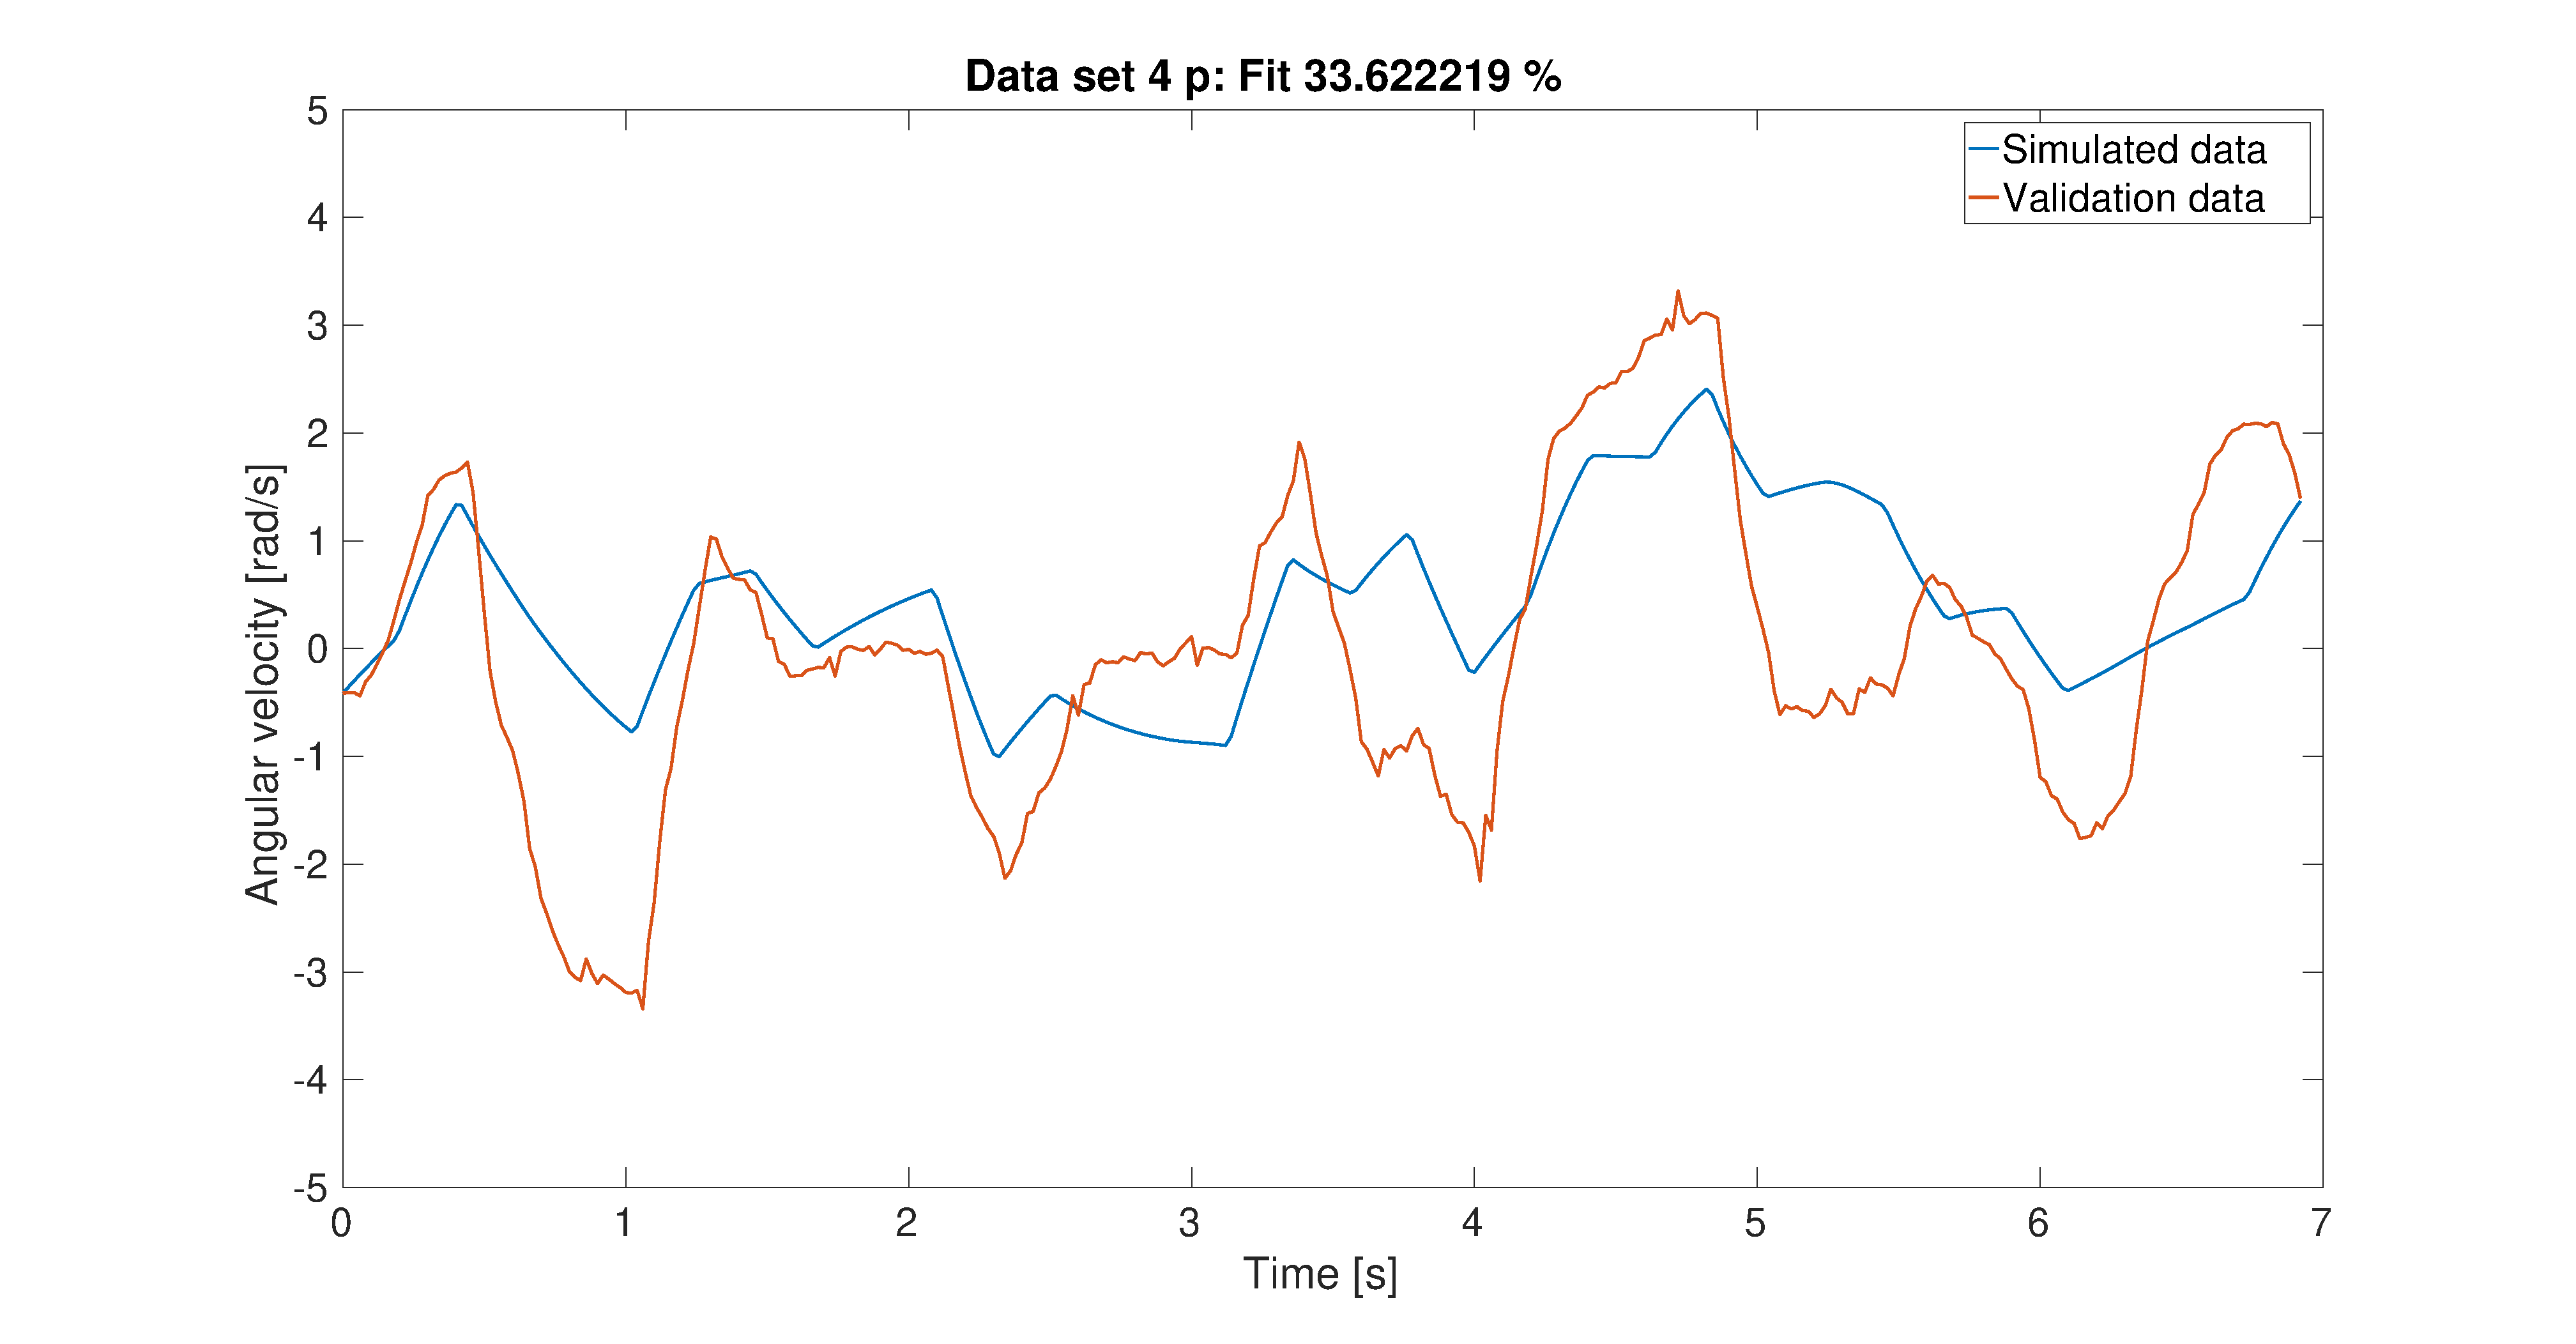
\includegraphics[width=0.7\textwidth]{ResultKalmanFixedMomentP}}
  \qquad
  \subfloat[][Comparison between a simulated model response and validation data in $q$.]{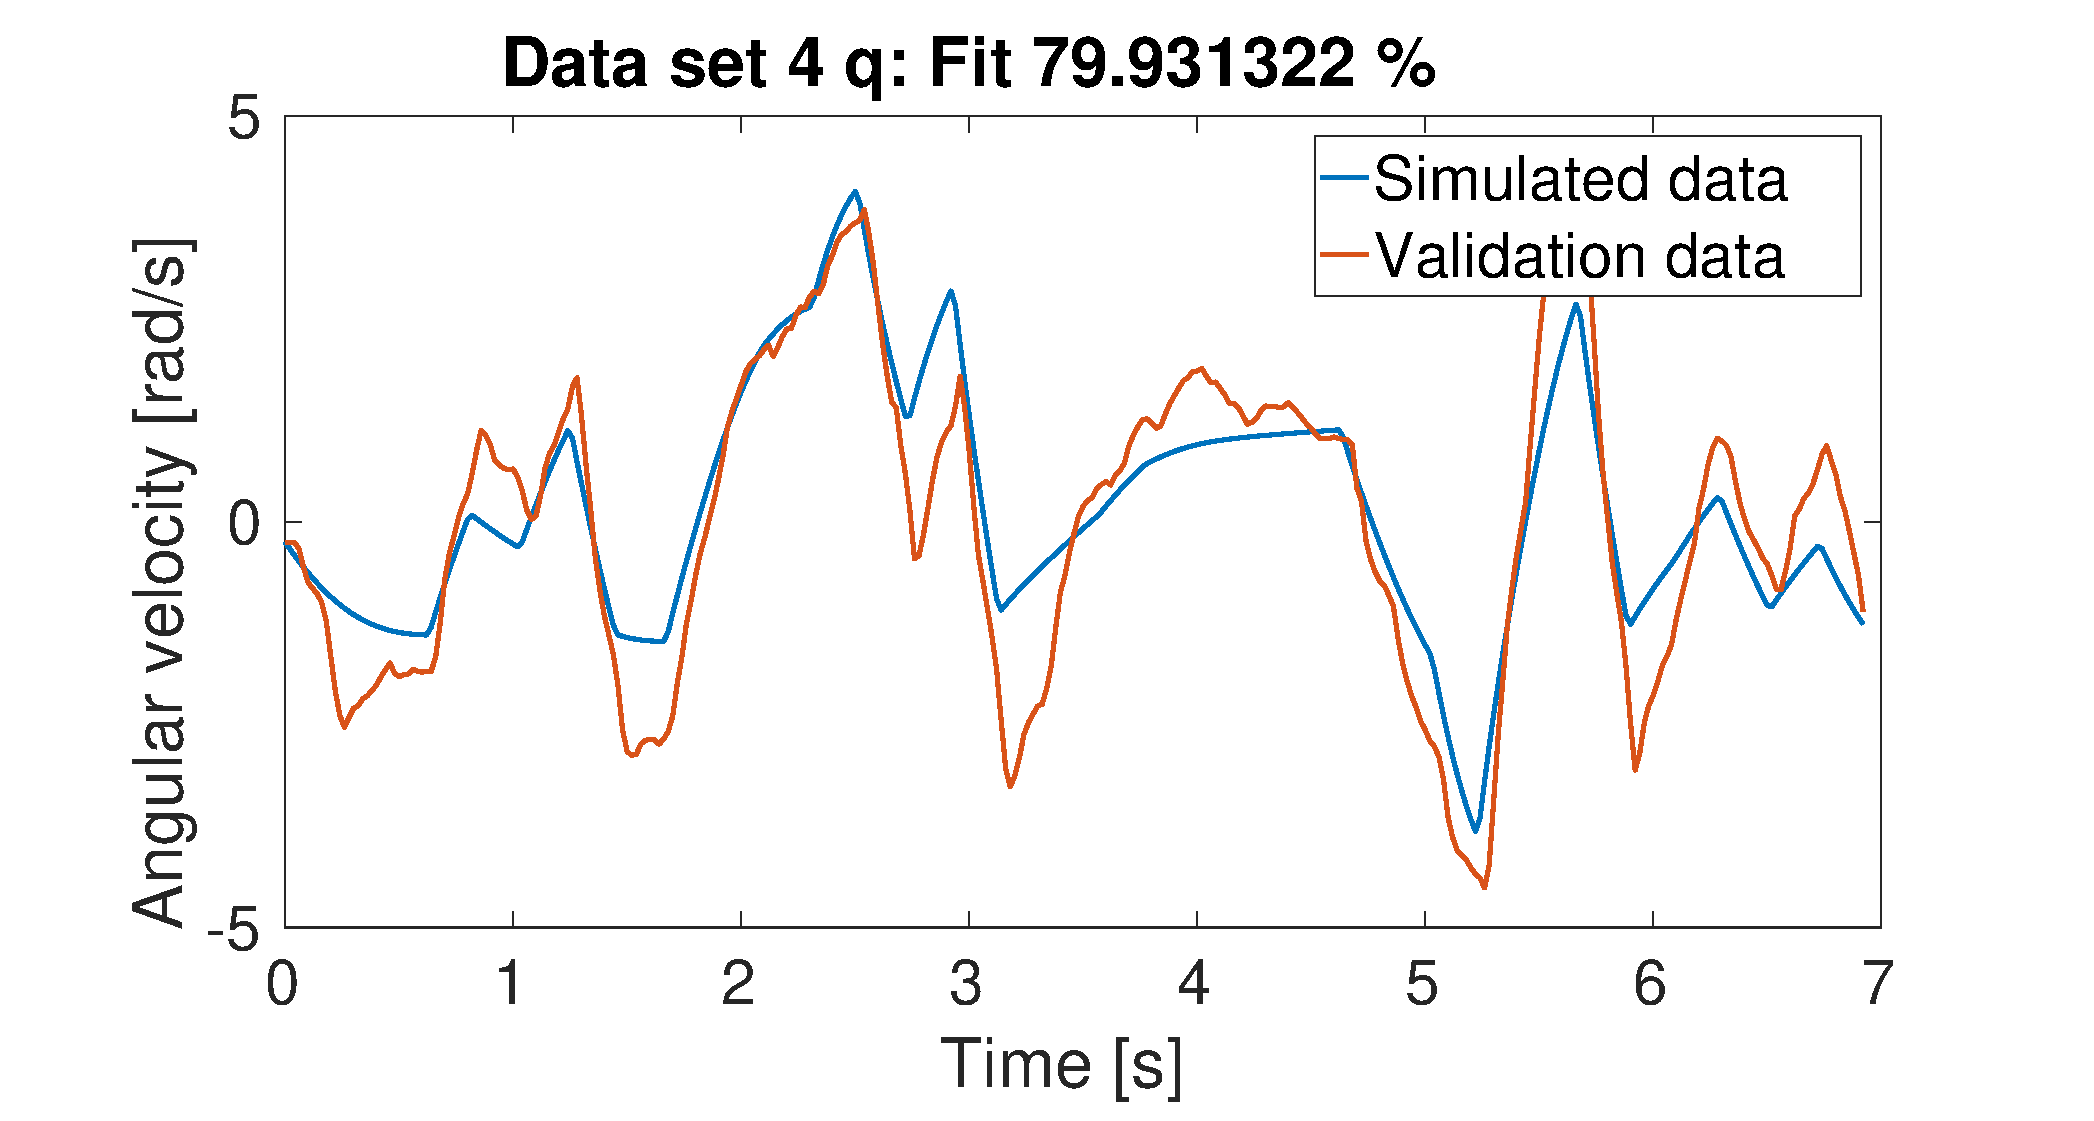
\includegraphics[width=0.7\textwidth]{ResultKalmanFixedMomentQ}}
  \\
  \subfloat[][Comparison between a simulated model response and validation data in $r$.]{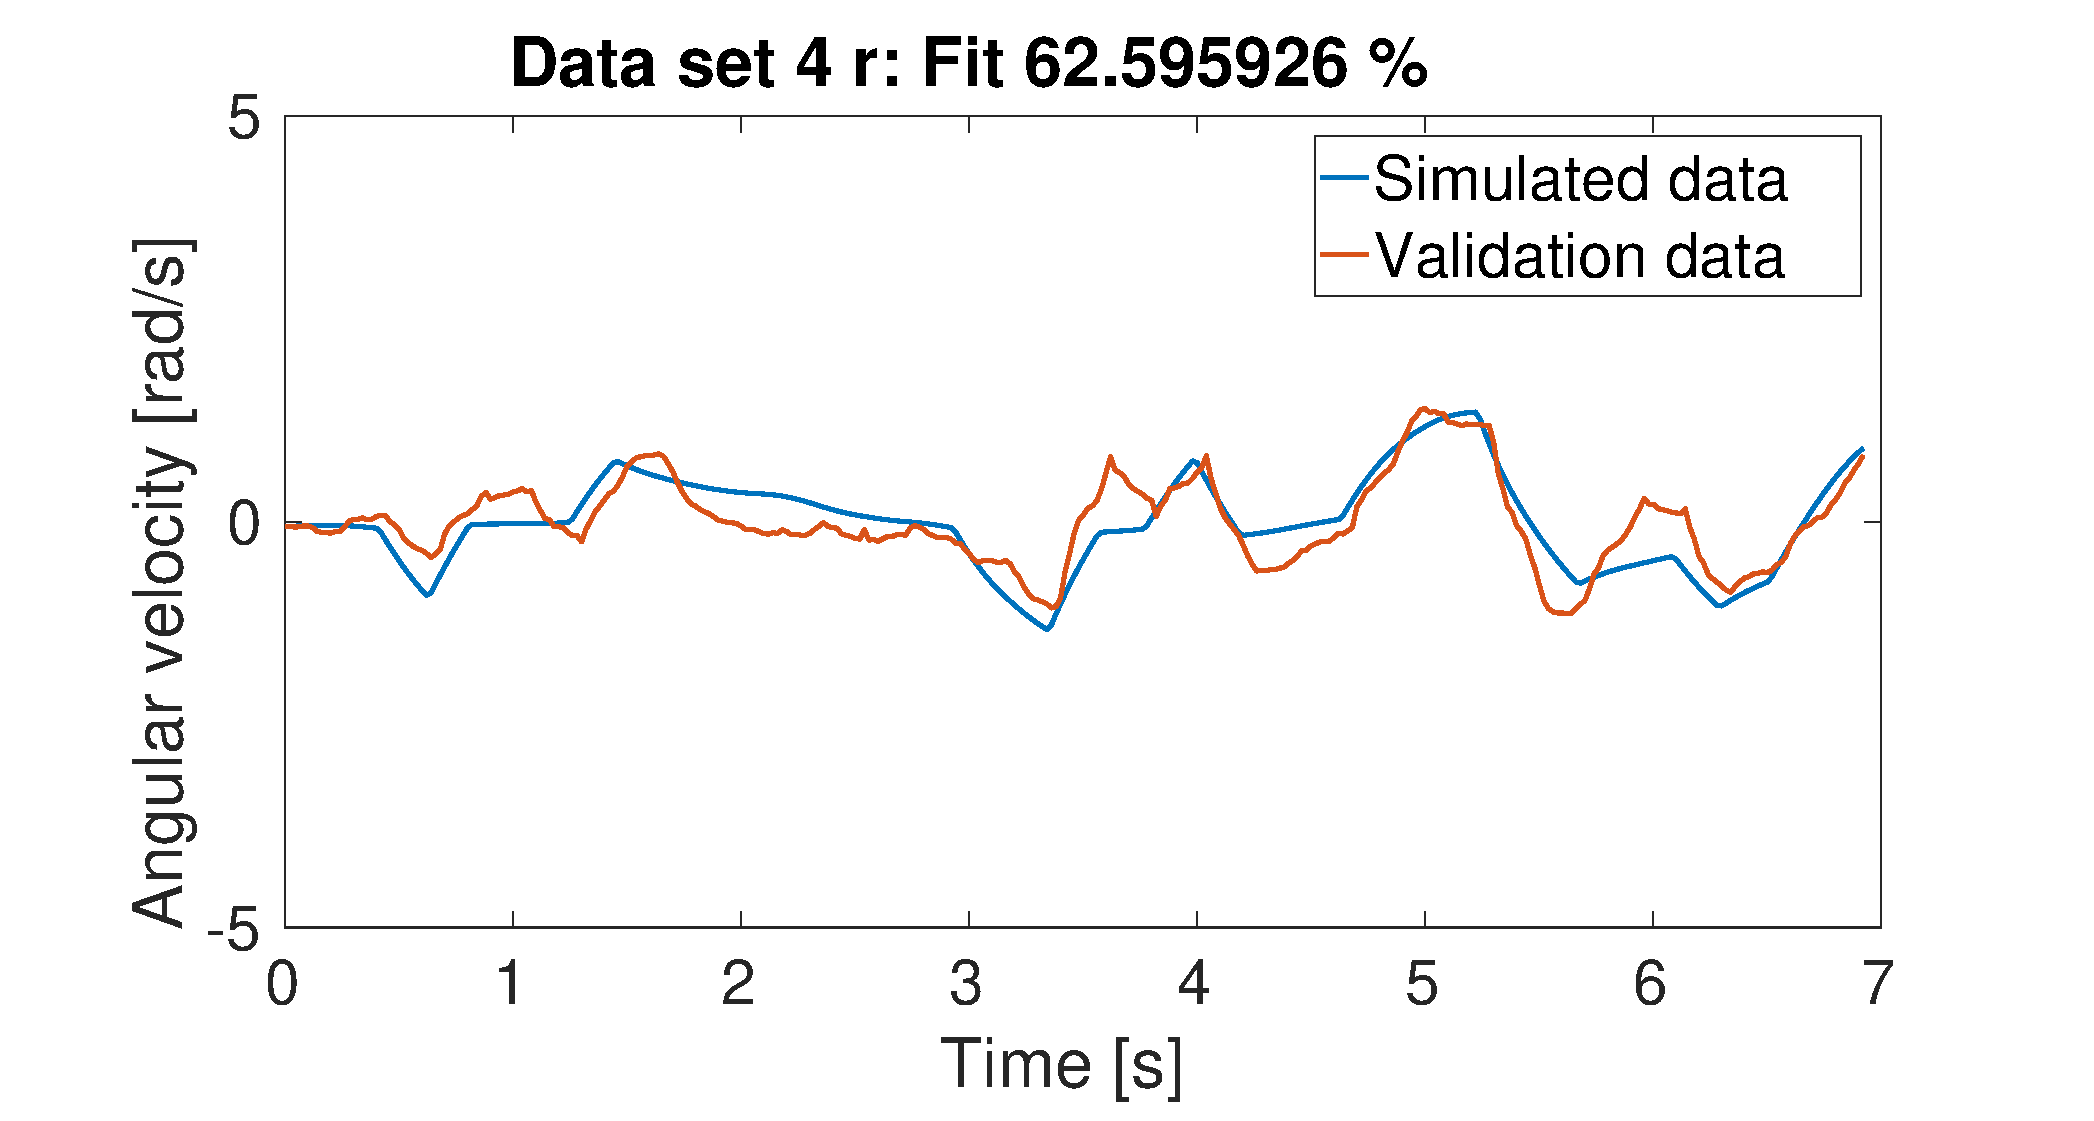
\includegraphics[width=0.7\textwidth]{ResultKalmanFixedMomentR}}
  \caption{\label{fig:ResultKalmanFixedMomentArms}%
    Comparison between simulation of $\nuVector$ (blue) with validation data (red). Moment-arm parameters are fixed. Goodness of fit statistic is displayed at the top of each sub-figure.}
\end{figure}

A second estimation was run using same model with the following settings
\begin{equation*}
\boldsymbol{Q}=\text{diag}[\underbrace{\overbrace{100}^{\times4}}_{\etaVector}... \underbrace{\overbrace{1000}^{\times3}}_{\nuVector}...\underbrace{\overbrace{0.01}^{\times3}}_{\boldsymbol{b}}... \underbrace{\overbrace{0.01}^{\times10}... \overbrace{0.000001}^{\times5}}_{\boldsymbol{\theta}}]\text{ ,}
\end{equation*}
\begin{equation*}
\boldsymbol{R} = \text{diag}[\underbrace{\overbrace{0.001}^{\times3}}_{\text{Gyro}}... \underbrace{\overbrace{0.1}^{\times3}}_{\text{Acc}}... \underbrace{\overbrace{100}^{\times3}}_{\text{mag}}]
\end{equation*}
The estimation was done with three data sets, of which the first two were used for estimation and the third for validation. Since these datasets were shorter the estimator was iterated five times, using the parameter values from the previous iteration as the new initial states. The resulting parameter values and their initial values can be viewed in \tableref{tab:ResultKalmanFixedMomentArmsLz6} and a comparison of a simulated run against validation data is shown in \figureref{fig:ResultKalmanFixedMomentArmsLz6}

% results kalman lz6=0 fixed moment arms
\begin{table}[hbp]
  \centering
  \caption{\label{tab:ResultKalmanFixedMomentArmsLz6}%
    The estimated parameters from the Kalman estimator method with moment arms fixed to measured values but with $\distance{z}{6}$ fixed to zero.}
  \begin{tabular}{l l p{0.25\linewidth}}
    \toprule%
    \textbf{Notation}  & \textbf{Starting Value} & \textbf{Estimated Value} \\
    \otoprule%   
    % Parameters that will be estimated
    $\etaVector$			&$[1\ 0\ 0\ 0]^T$					&\\
    $\nuVector$			&$[0\ 0\ 0]^T$						&\\
    $\boldsymbol{b}$					&$[0\ 0\ 0]^T$			&\\
	$z_B$               & -0.05	\meter 						& -0.0606  	\meter\\
    $\Kp$               & -1   	\kilogram\usk\meter\squared 	& -0.8745 		\kilogram\usk\meter\squared\\
    $\Kpabsp$           & -1  	\kilogram\usk\meter\squared	& -0.6279  		\kilogram\usk\meter\squared\\
    $\Mq$               & -1  	\kilogram\usk\meter\squared	& -0.8529  		\kilogram\usk\meter\squared\\
    $\Mqabsq$           & -1  	\kilogram\usk\meter\squared	& -0.2505  	\kilogram\usk\meter\squared\\
    $\Nr$               & -1  	\kilogram\usk\meter\squared	& -1.0469		\kilogram\usk\meter\squared\\
    $\Nrabsr$           & -1  	\kilogram\usk\meter\squared	& -1.0405 		\kilogram\usk\meter\squared\\
    $A_p$               & 1 	\kilogram\usk\meter\squared	&  0.9728 		\kilogram\usk\meter\squared\\
    $B_q$               & 1 	\kilogram\usk\meter\squared	&  0.7266		\kilogram\usk\meter\squared\\
    $C_r$               & 1 	\kilogram\usk\meter\squared	&  1.2013		\kilogram\usk\meter\squared\\
    $\distance{x}{1}$  &0.19 \meter & 0.19 \meter\\
    $\distance{y}{1}$  &0.11 \meter & 0.1102 \meter\\
    $\distance{x}{2}$  &0.19 \meter & 0.19 \meter\\
    $\distance{y}{2}$  &0.11 \meter & 0.1102 \meter\\
    $\distance{y}{3}$  &0.11 \meter & 0.11 \meter\\
    $\distance{x}{5}$  &0.17 \meter & 0.1701 \meter\\
    $\distance{y}{4}$  &0.11 \meter & 0.11 \meter\\
    $\distance{z}{6}$  &0.0 \meter & 0.0 \meter\\ 
    \bottomrule%
  \end{tabular}
\end{table}

% results kalman lz6=0 fixed moment arms
\begin{figure}[tbp]
  \centering
  \subfloat[][Comparison between a simulated model response and validation data in $p$.]{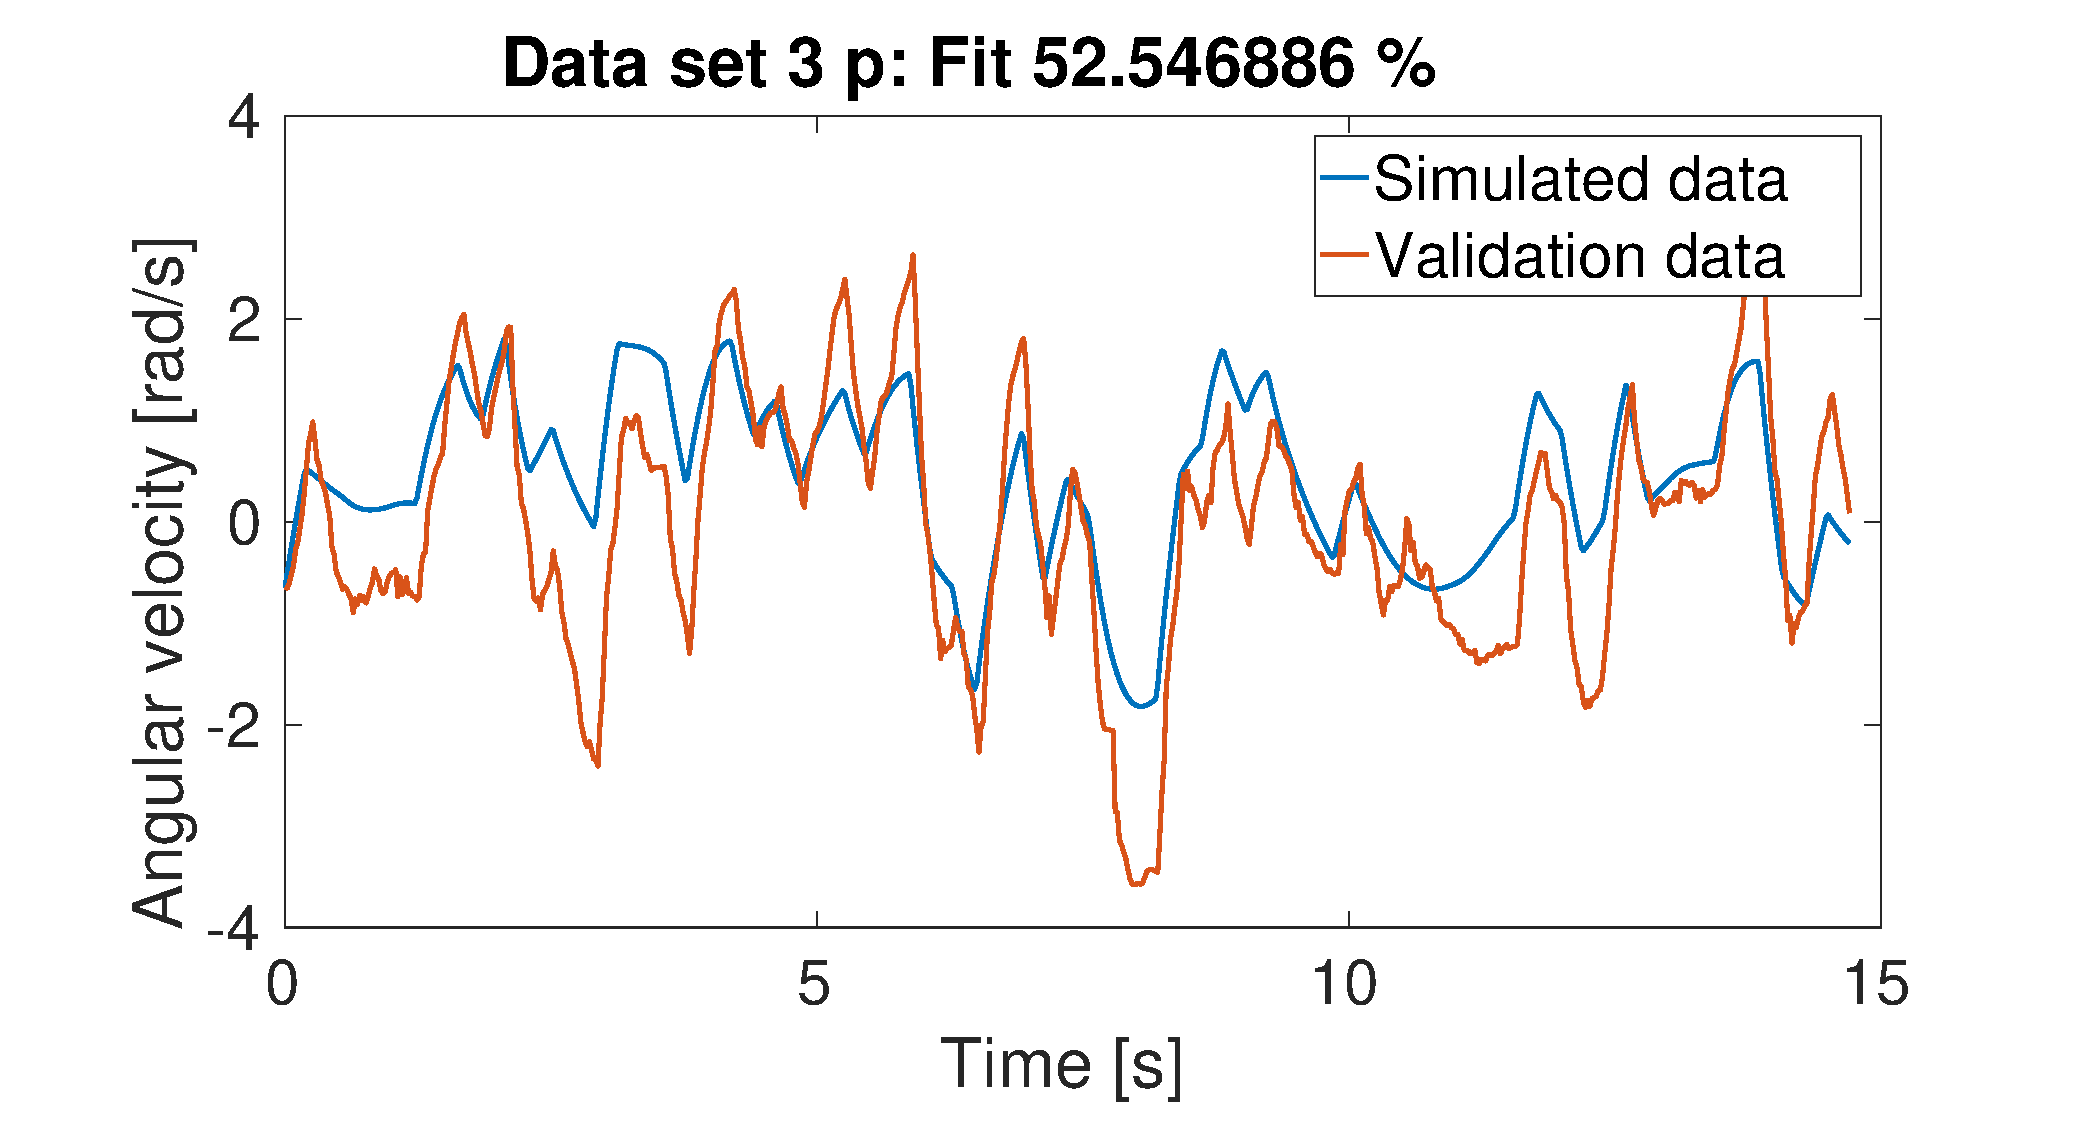
\includegraphics[width=0.7\textwidth]{ResultKalmanFixedMomentPLz0}}
  \qquad
  \subfloat[][Comparison between a simulated model response and validation data in $q$.]{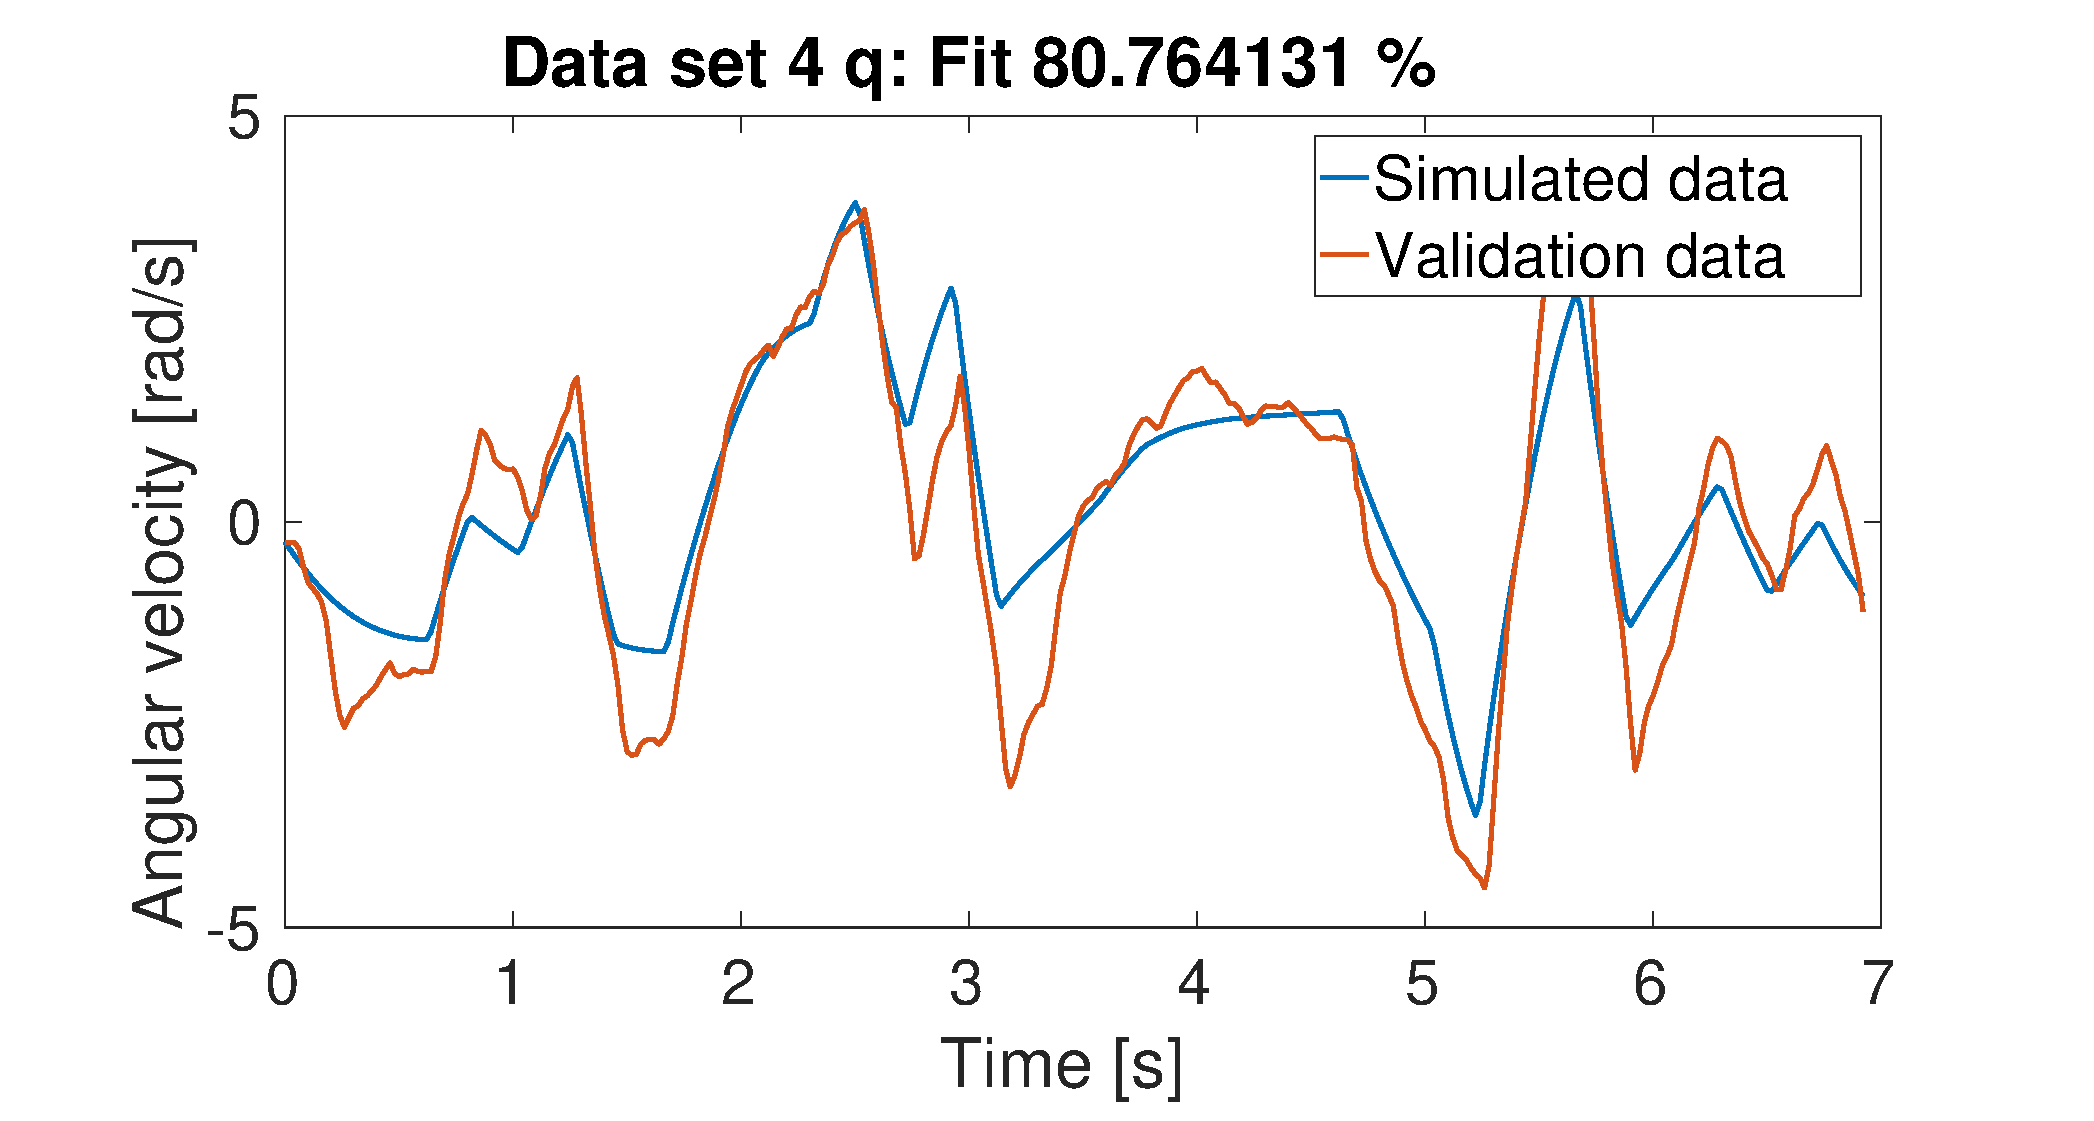
\includegraphics[width=0.7\textwidth]{ResultKalmanFixedMomentQLz0}}
  \\
  \subfloat[][Comparison between a simulated model response and validation data in $r$.]{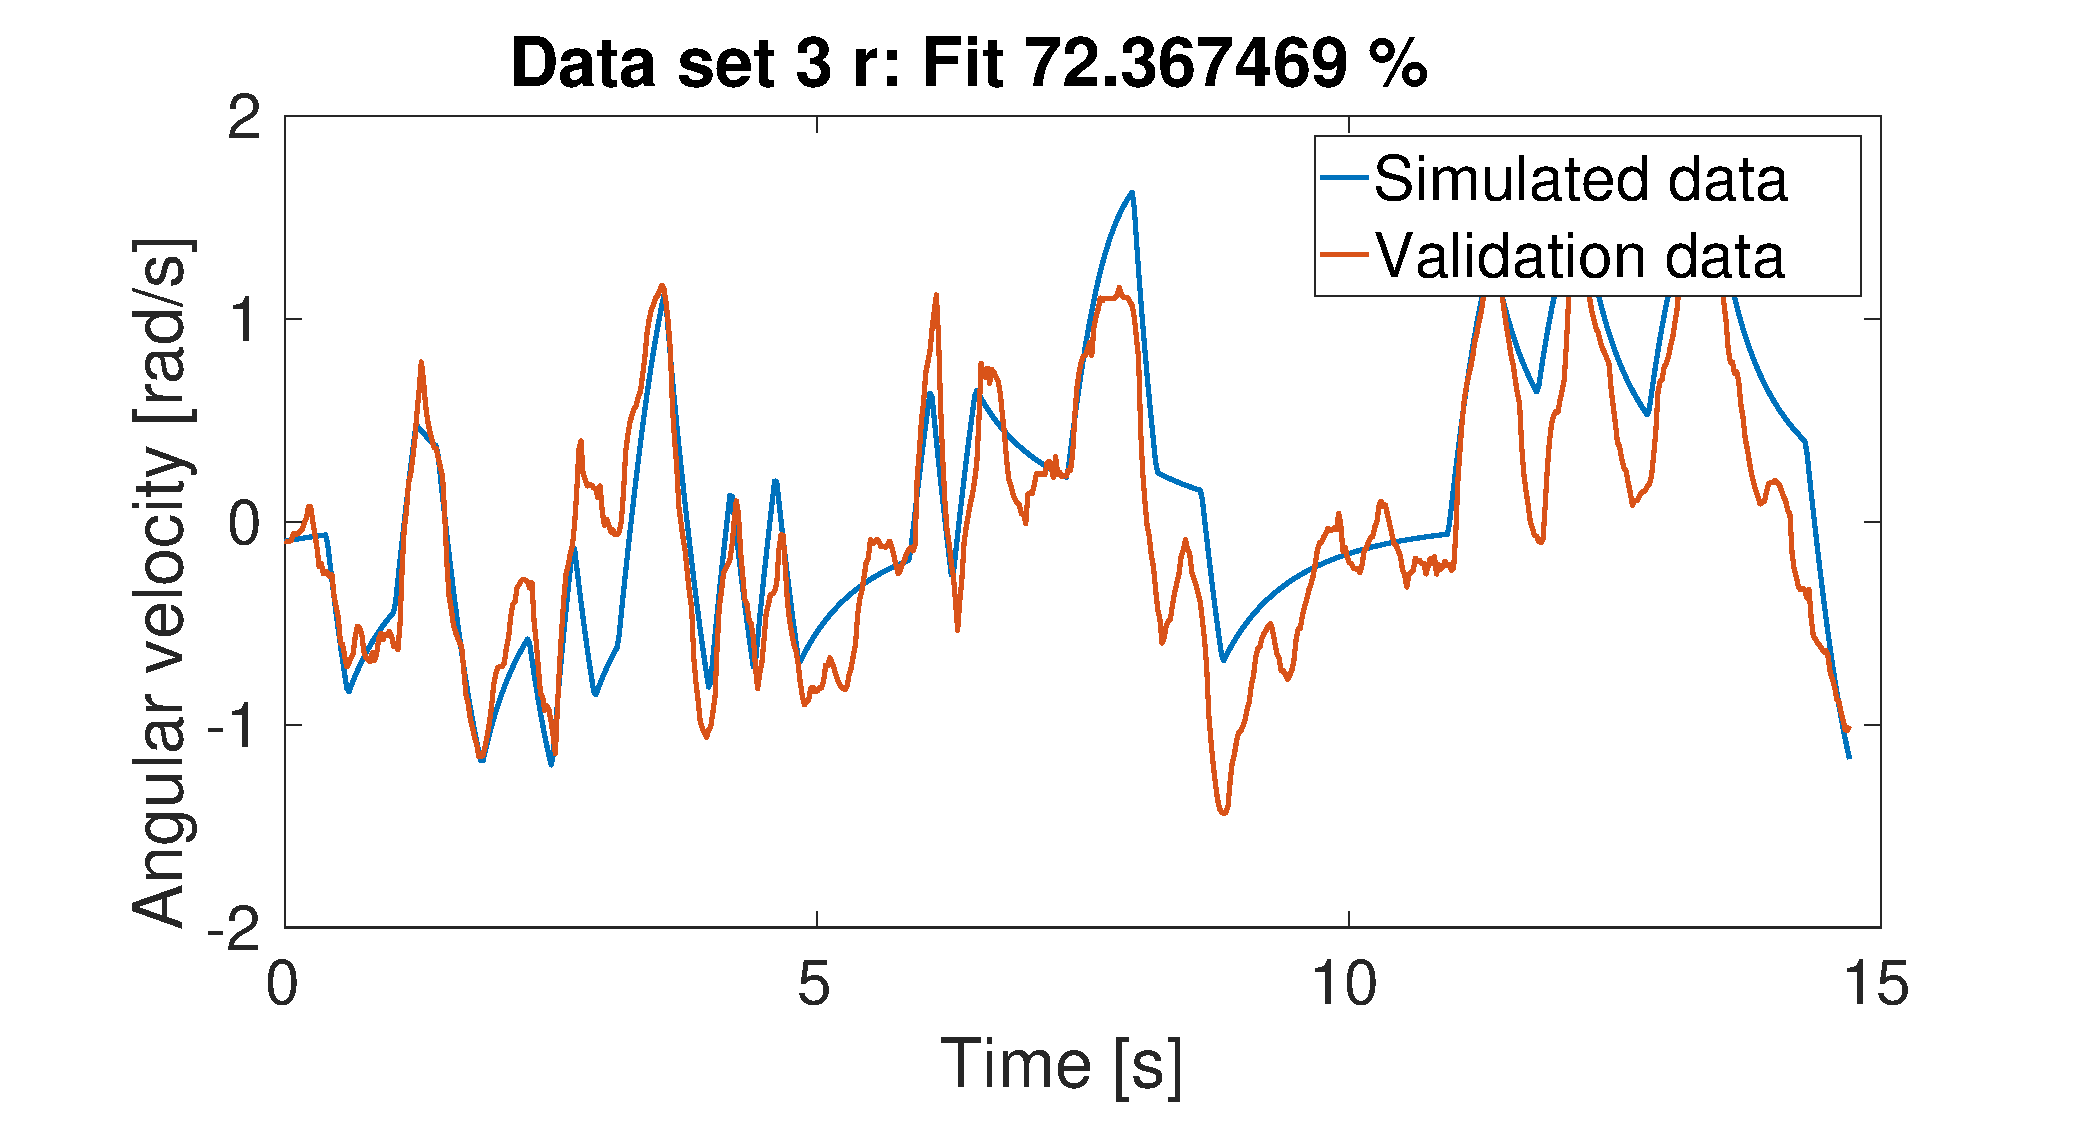
\includegraphics[width=0.7\textwidth]{ResultKalmanFixedMomentRLz0}}
  \caption{\label{fig:ResultKalmanFixedMomentArmsLz6}%
    Comparison between simulation of $\nuVector$ (blue) with validation data (red). Moment-arm parameters are fixed and \distance{z}{6} is set to zero. Goodness of fit statistic is displayed at the top of each sub-figure.}
\end{figure}


\section{Discussion}
To estimate parameters in the reduced 6-\abbrDOF model was harder than it at first seemed. When using the error-prediction method problems were encountered with bad fit in $p$ and the estimate of $\etaVector$ did not follow the kinematic relations described in \sectionref{sec:coordinates}. The problem with $\etaVector$ not following the kinematic relations was further investigated by comparing integration of \eqref{eq:eulerAnglesdot} with $\hat{\etaVector}$ from the sensor fusion. As can be seen in \Figureref{fig:integratedAngleVelocities} the result was not satisfactory, with the estimated angles and the integration of \eqref{eq:eulerAnglesdot} being very dissimilar. It was therefore concluded that the estimated angles were unfit for use as outputs during parameter estimation unless a new motion model for the sensor fusion was created to solve the issue. It is therefore recommended that the validity of the observer is controlled using relations such as those in \sectionref{sec:coordinates} before collecting data. 

\begin{figure}[htbp]
  \centering
  \subfloat[][\label{fig:velocityAnglePhi}Comparison between integration of $\dot{\phi}$ and $\hat{\phi}$ from the \abbrEKF]{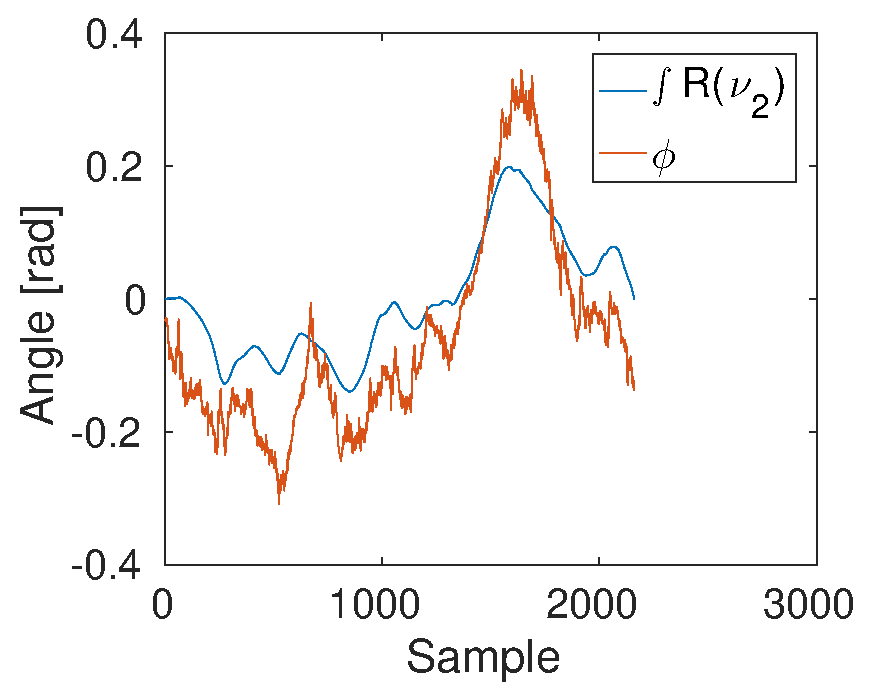
\includegraphics[width=0.7\textwidth]{velocityAnglePhi}}
  \qquad
  \subfloat[][\label{fig:velocityAngleTheta}Comparison between integration of $\dot{\theta}$ and $\hat{\theta}$ from the \abbrEKF]{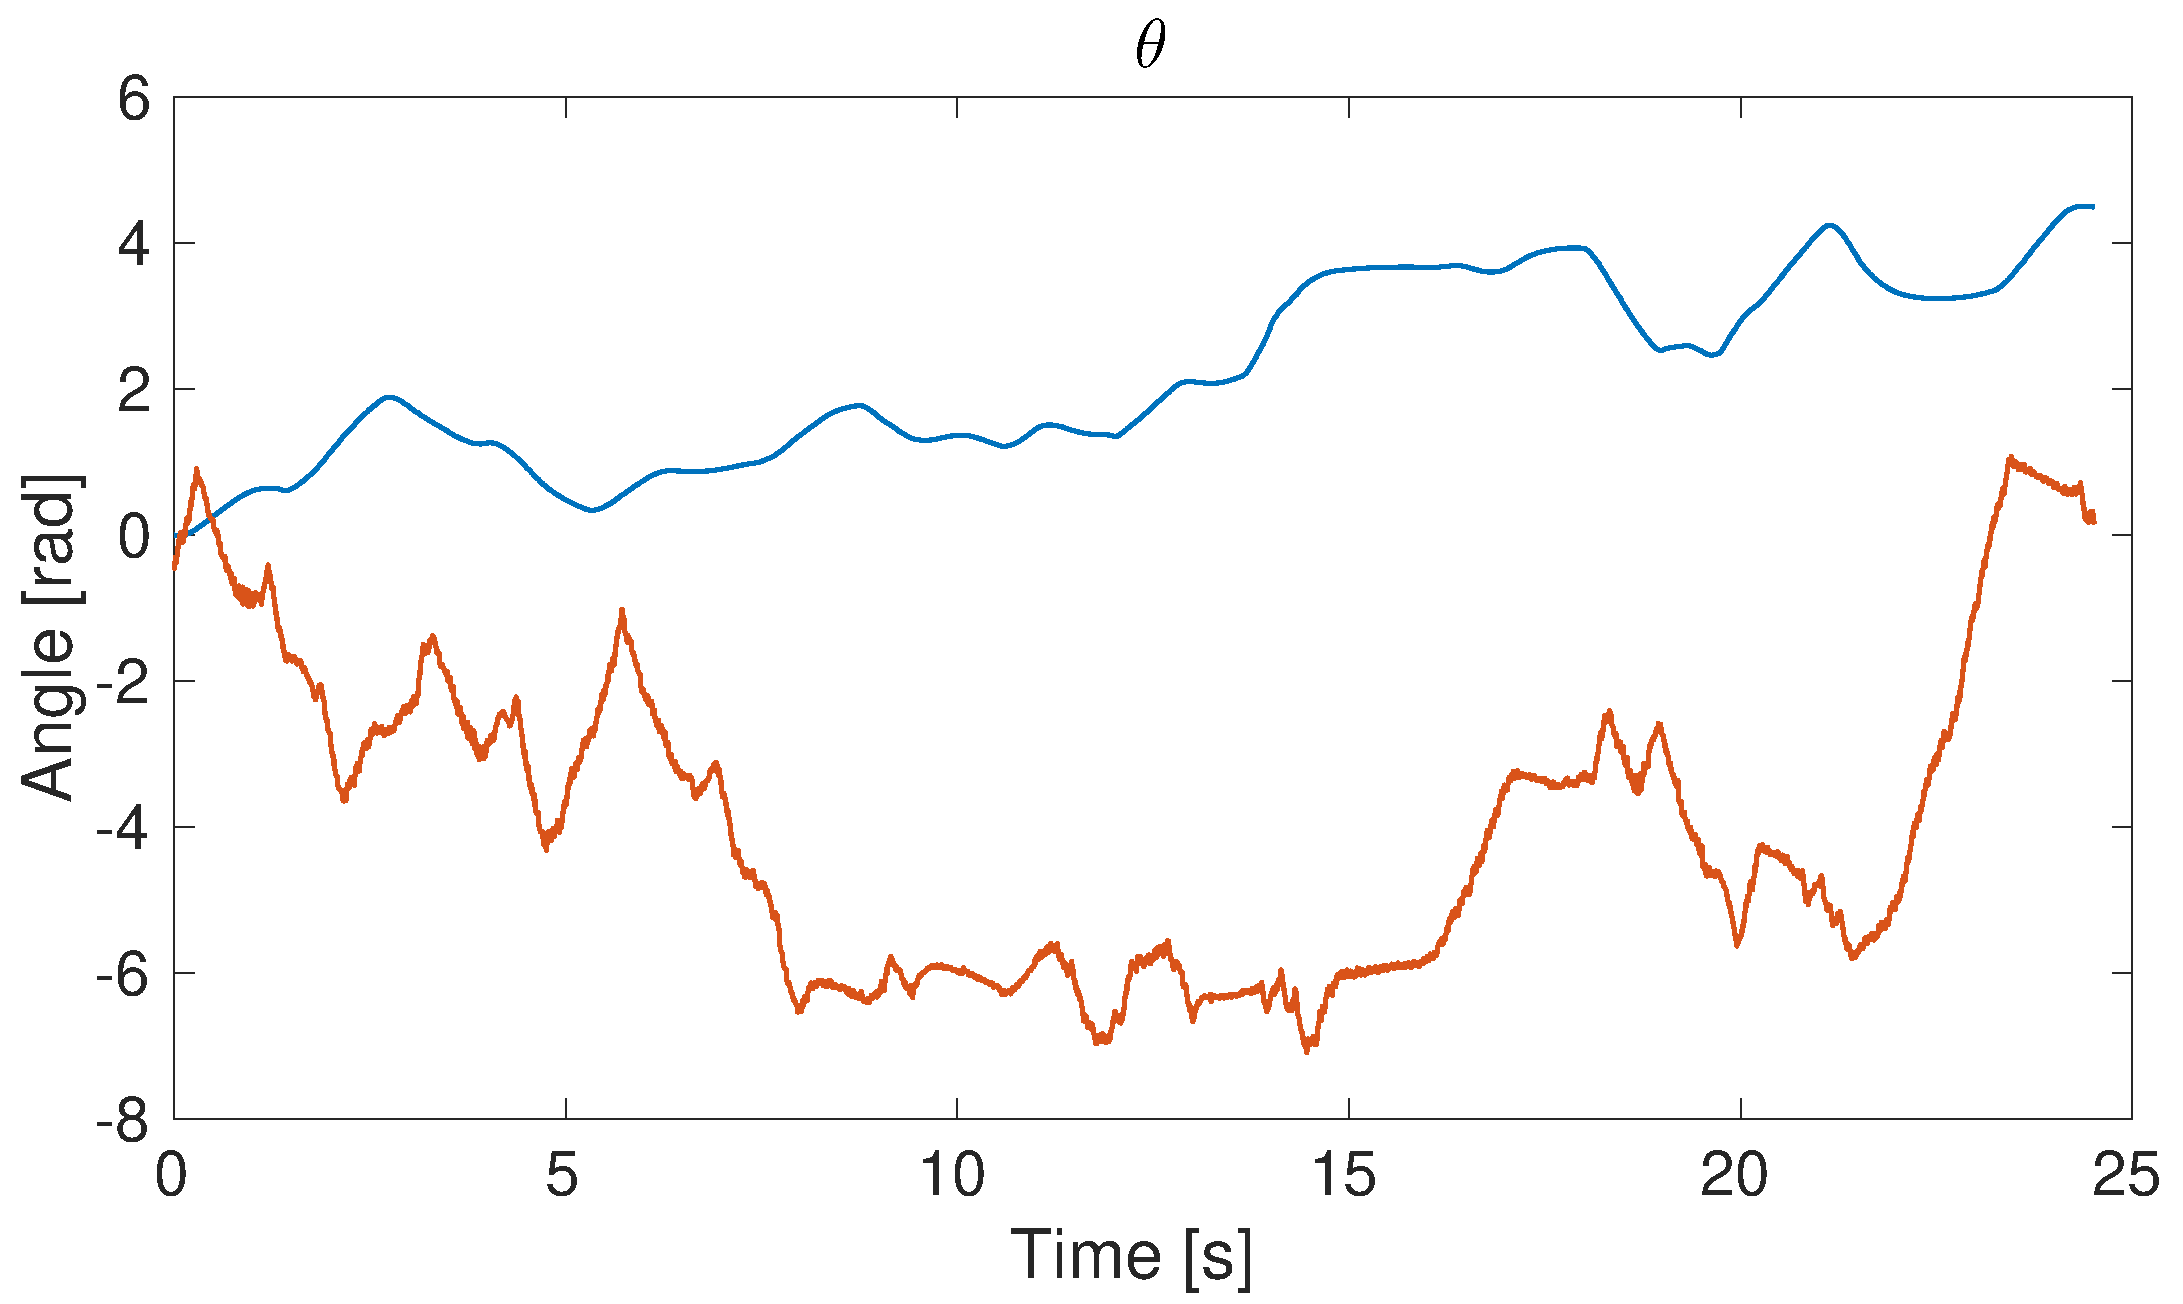
\includegraphics[width=0.7\textwidth]{velocityAngleTheta}}
  \\
  \subfloat[][\label{fig:velocityAnglePsi}Comparison between integration of $\dot{\psi}$ and $\hat{\psi}$ from the \abbrEKF]{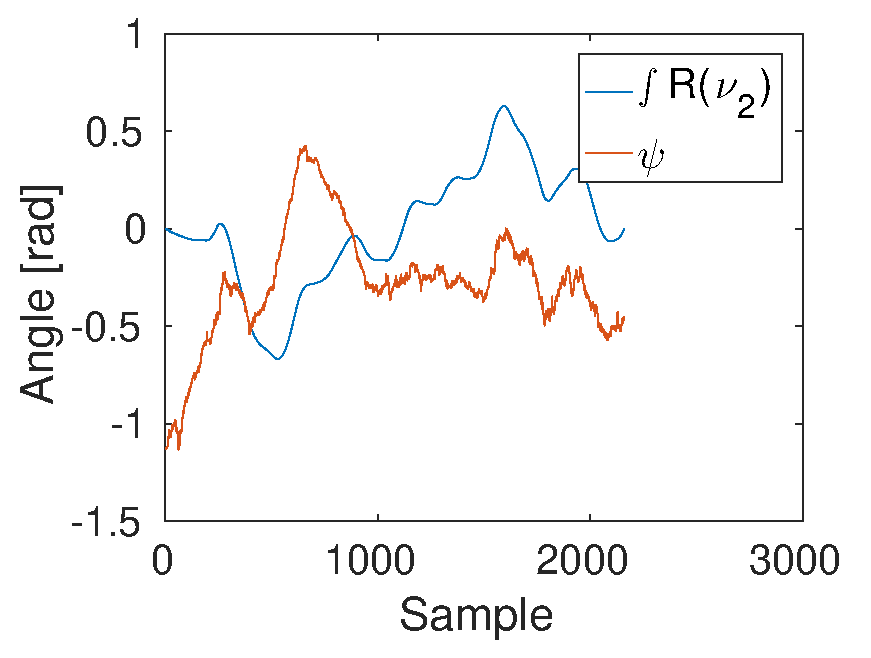
\includegraphics[width=0.7\textwidth]{velocityAnglePsi}}
  \caption{\label{fig:integratedAngleVelocities}%
  A comparison between integration of euler angles (blue) using \eqref{eq:eulerAnglesdot} and the estimated euler angles from the \abbrEKF (red). The angles are poorly estimated and thus not suitable to use as outputs in parameter estimation.}
\end{figure}

Another issue that was encountered when using the prediction-error method was that when angular velocities and linear accelerations were used as outputs, the model was extremely sensitive to the initial value of $\etaVector$. This was even more complicated since the model was modified to use quaternions to represent the \abbrROV's attitude. To examine this problem further data was generated using a simulator and the simulated data was used in the prediction-error method. The estimator was initialised with the correct initial parameter values from the simulator, but it was free to estimate the initial value of the quaternions. As expected, the estimated starting quaternion was not well estimated, which in turn led to the parameters diverging from their true values and a low fit was obtained. A result from such a test can be seen in \Figureref{fig:angVelSim}.

\begin{figure}[htbp]
  \centering %comparison betwwen two simulations
  \subfloat[][\label{fig:angVelSimp}Comparison of simulated angular velocity around the \abbrROV's x-axis with simulated validation data.]{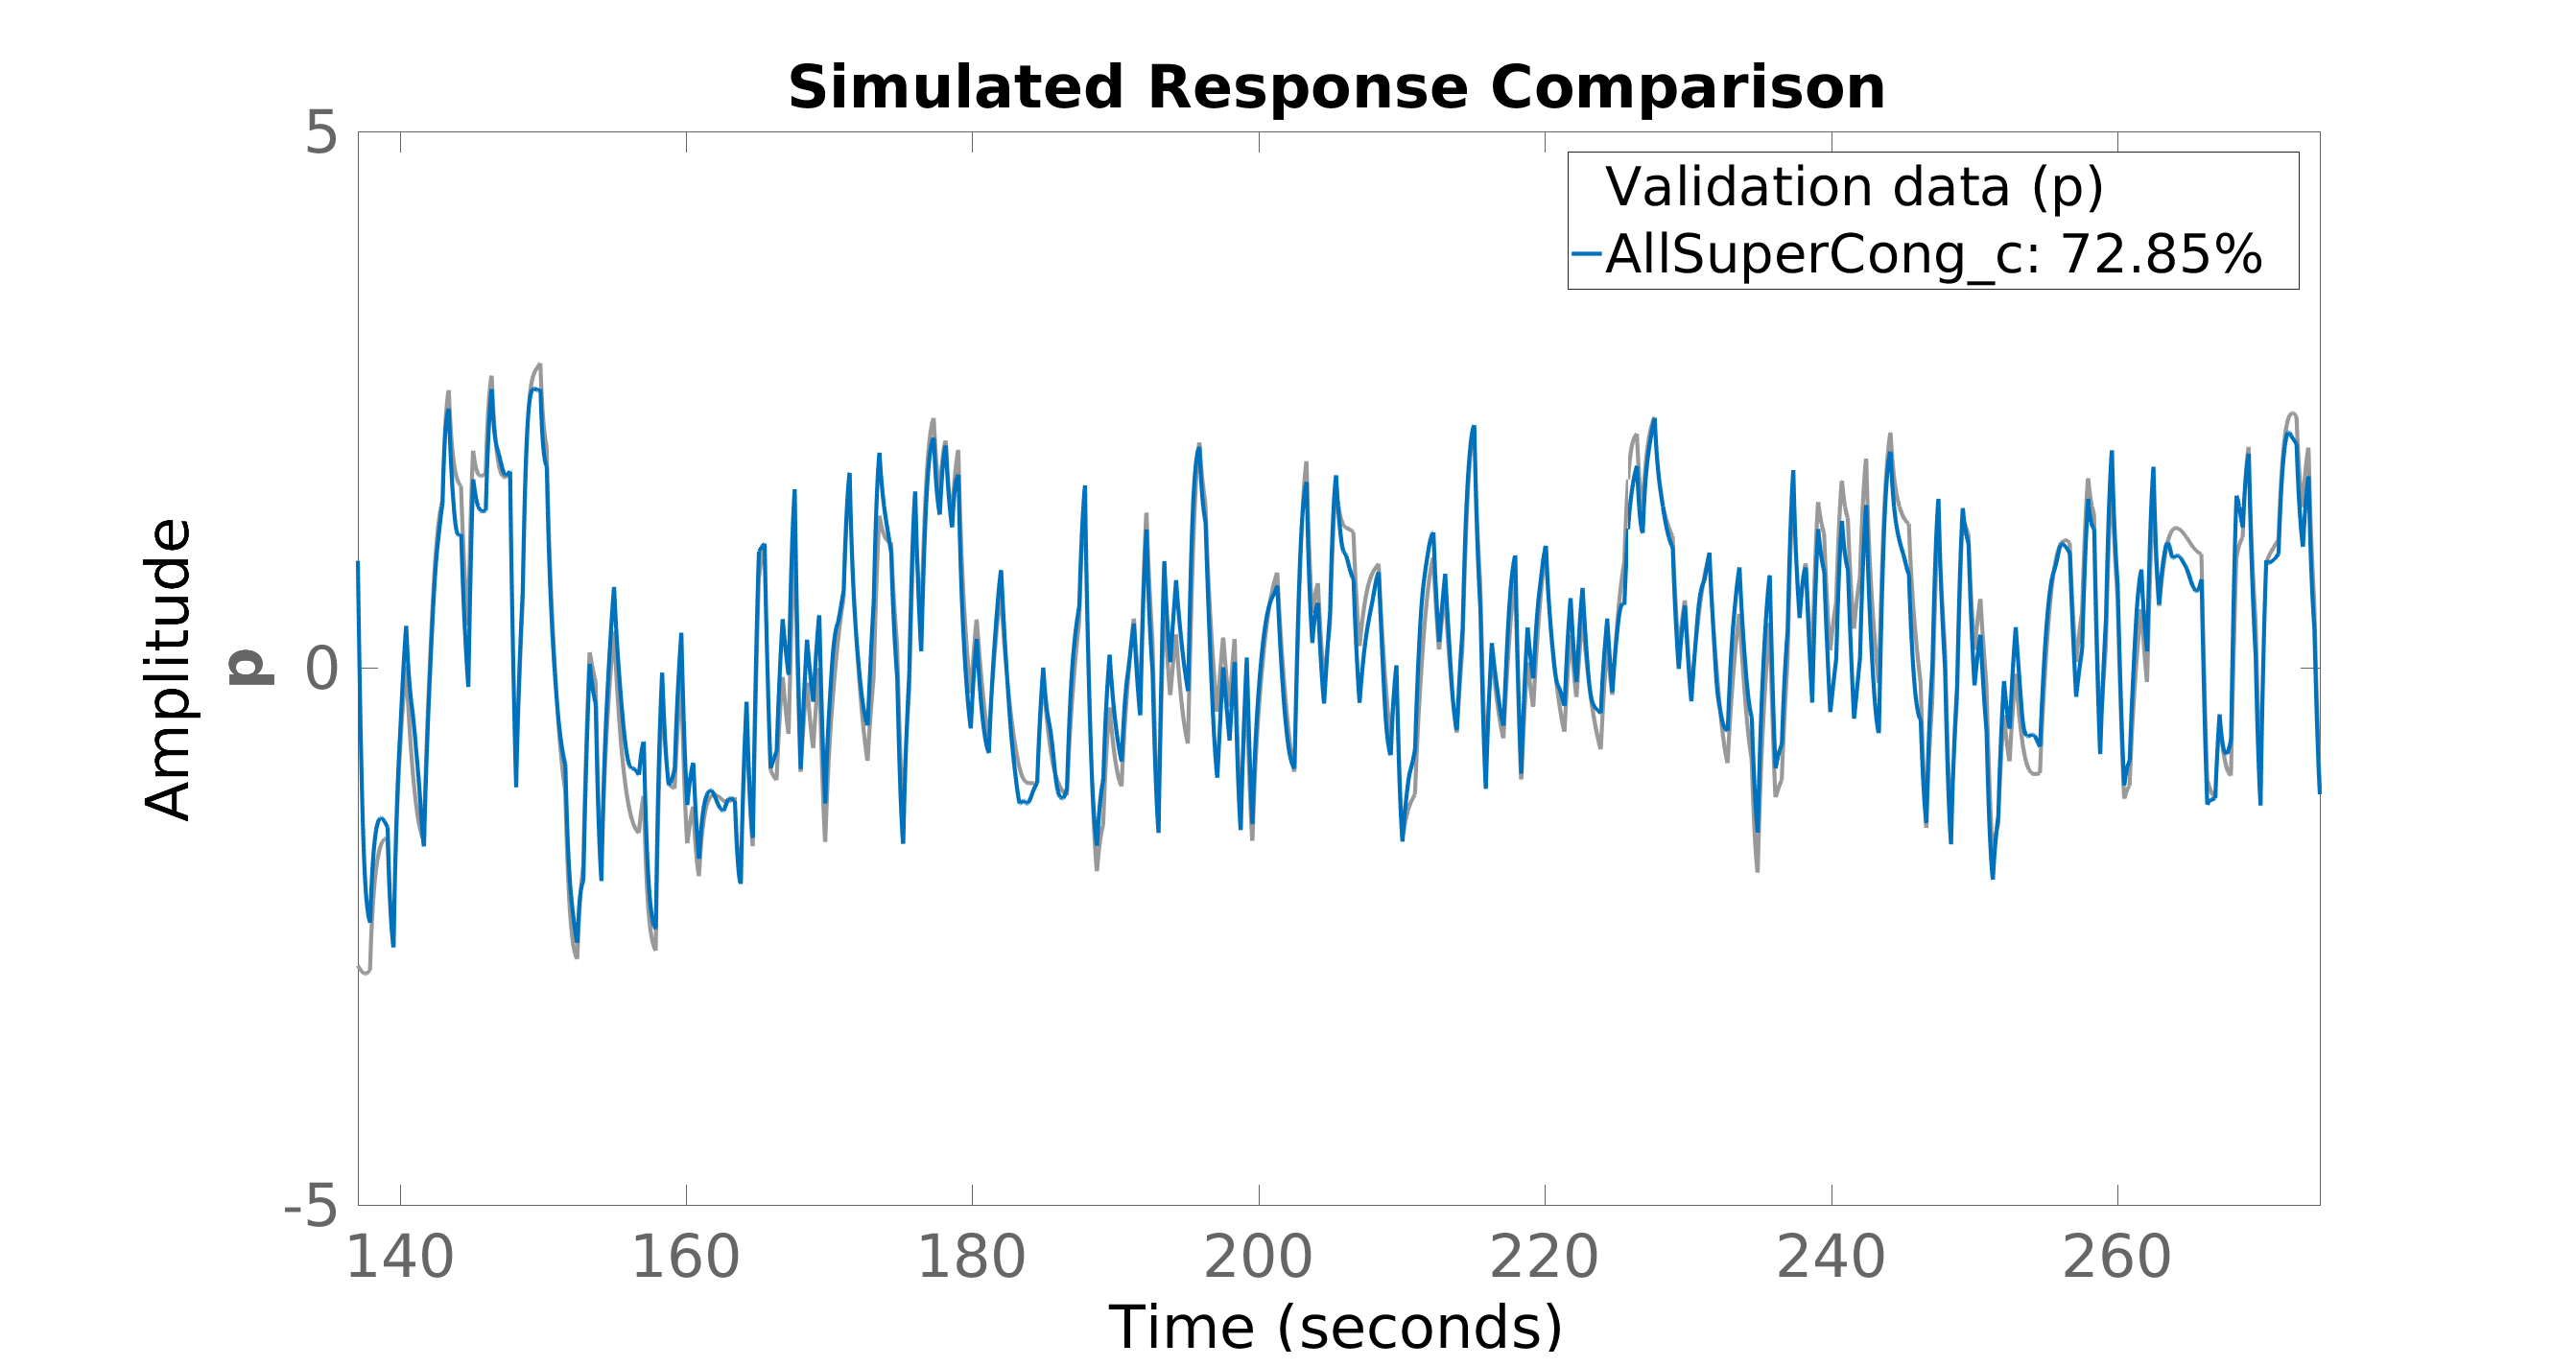
\includegraphics[width=0.4\textwidth]{angVelSimp}}
  \qquad
  \subfloat[][\label{fig:angVelSimq}Comparison of simulated angular velocity around the \abbrROV's y-axis with simulated validation data.]{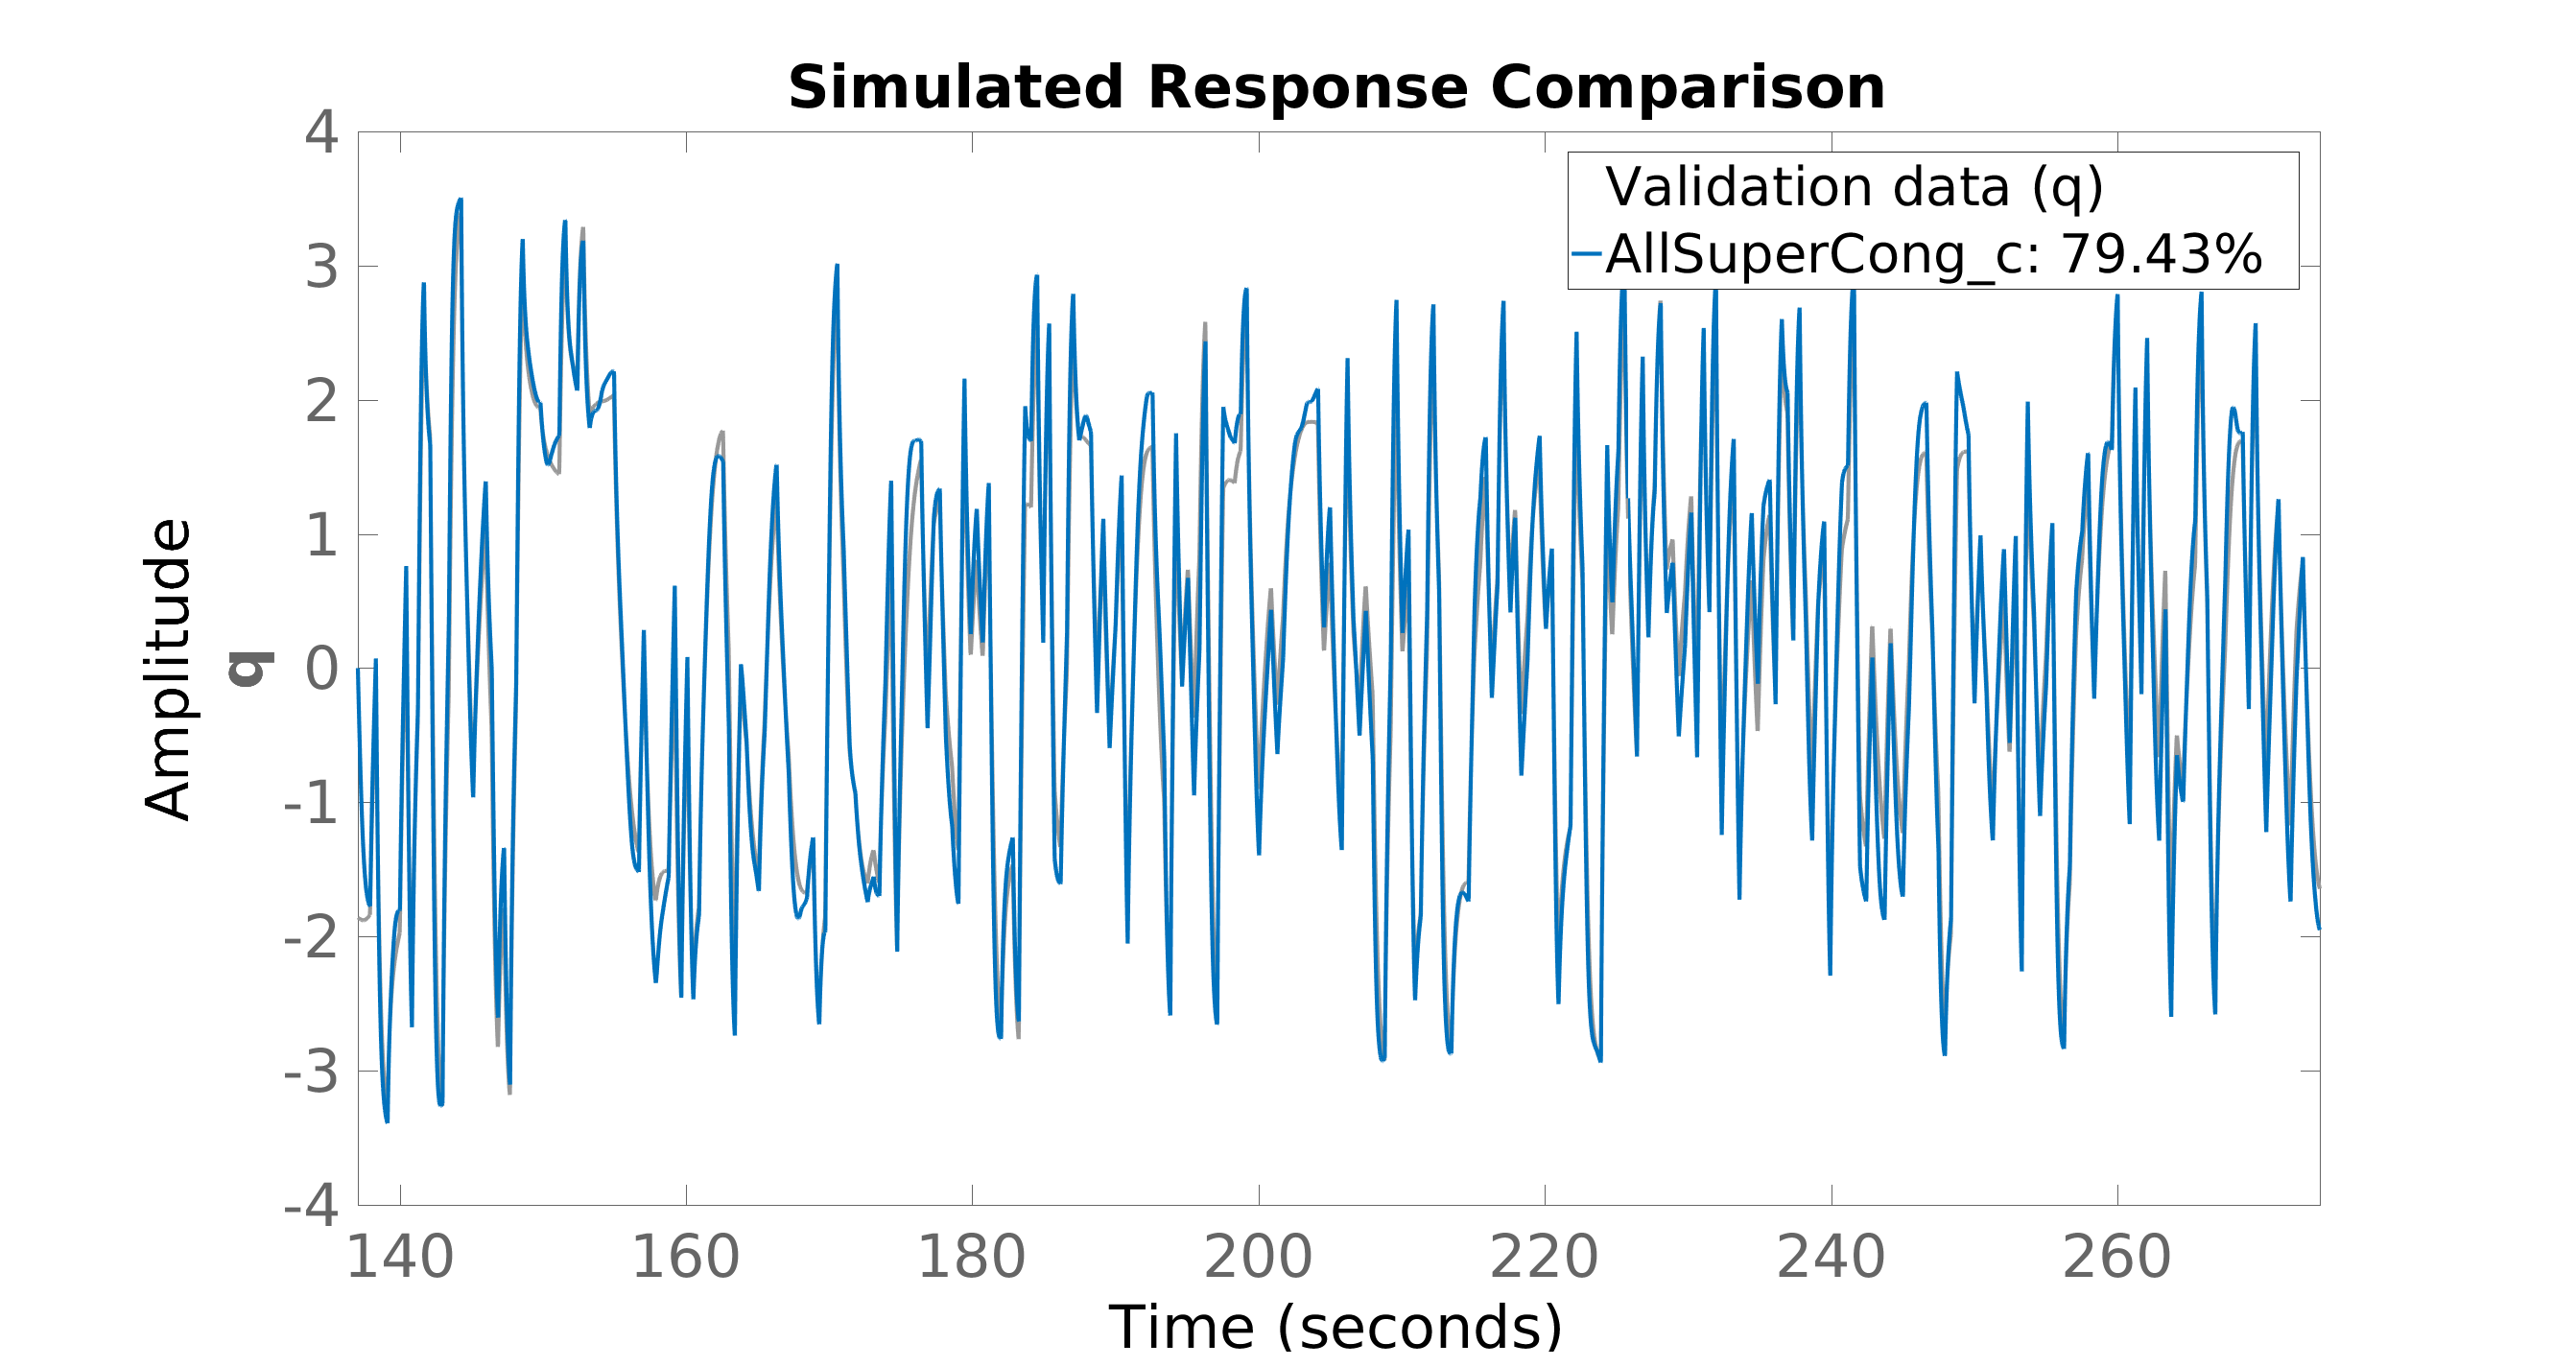
\includegraphics[width=0.4\textwidth]{angVelSimq}}
  \qquad
  \subfloat[][\label{fig:angVelSimr}Comparison of simulated angular velocity around the \abbrROV's z-axis with simulated validation data.]{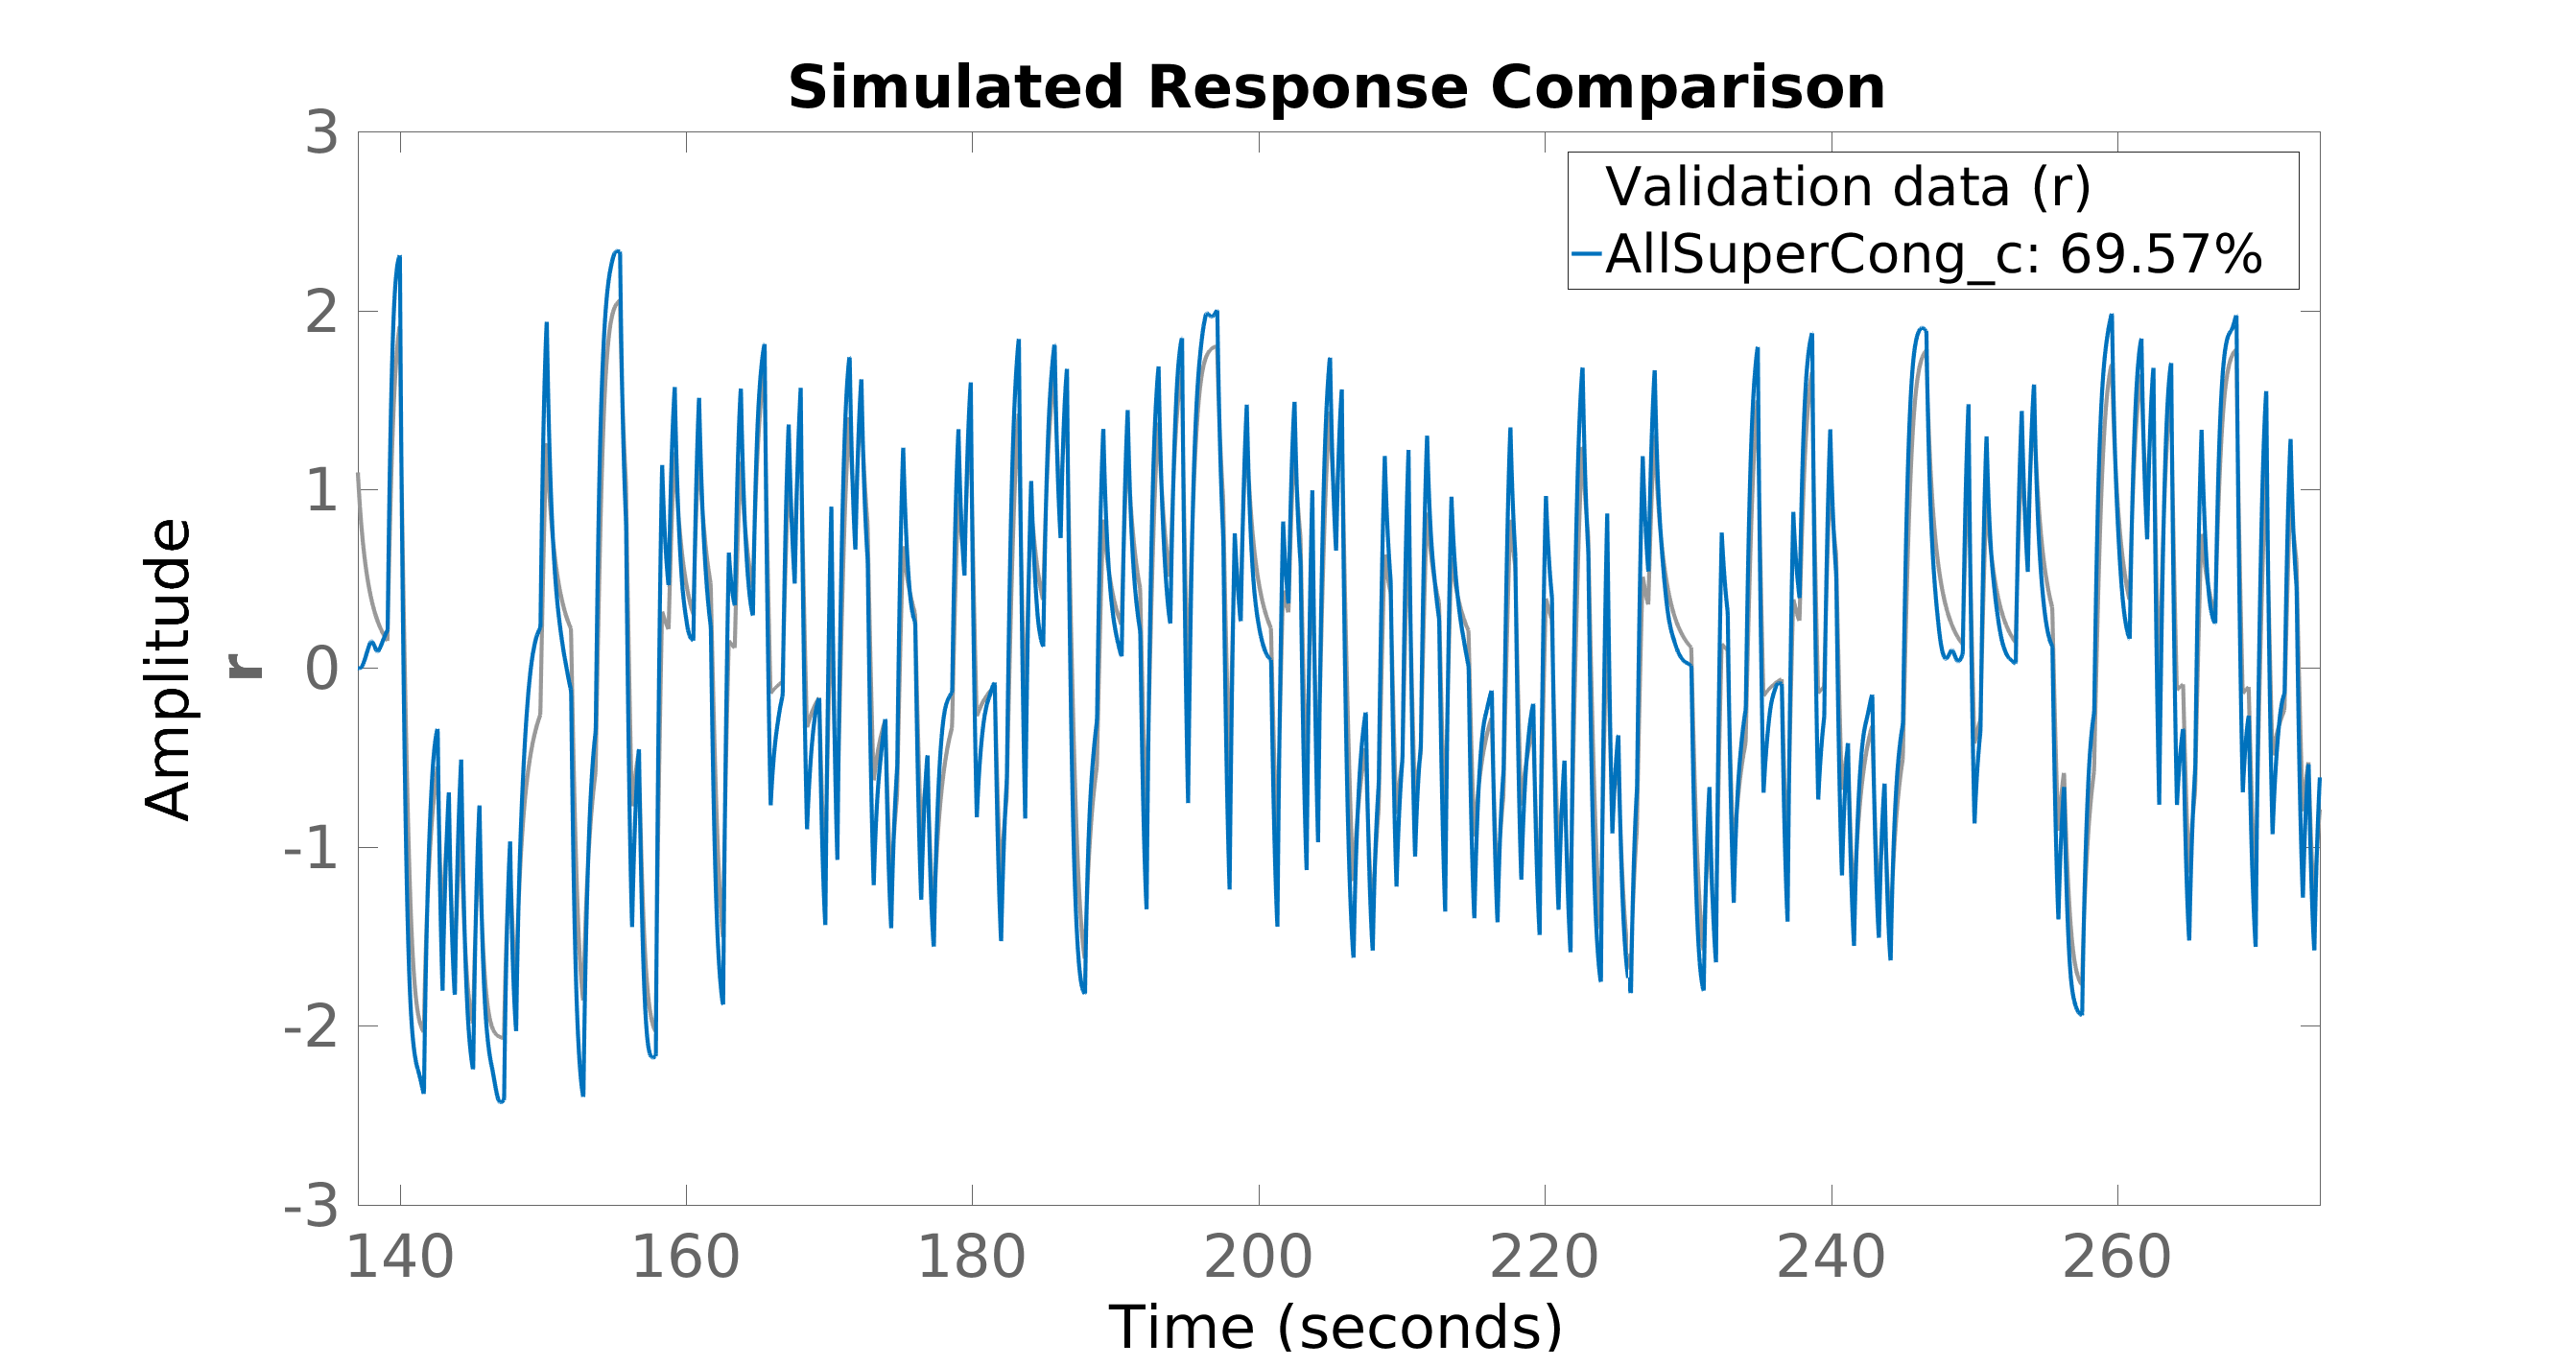
\includegraphics[width=0.4\textwidth]{angVelSimr}}
    \qquad
  \subfloat[][\label{fig:linAccSimx}Comparison of simulated linear acceleration in the \abbrROV's x-axis with simulated validation data.]{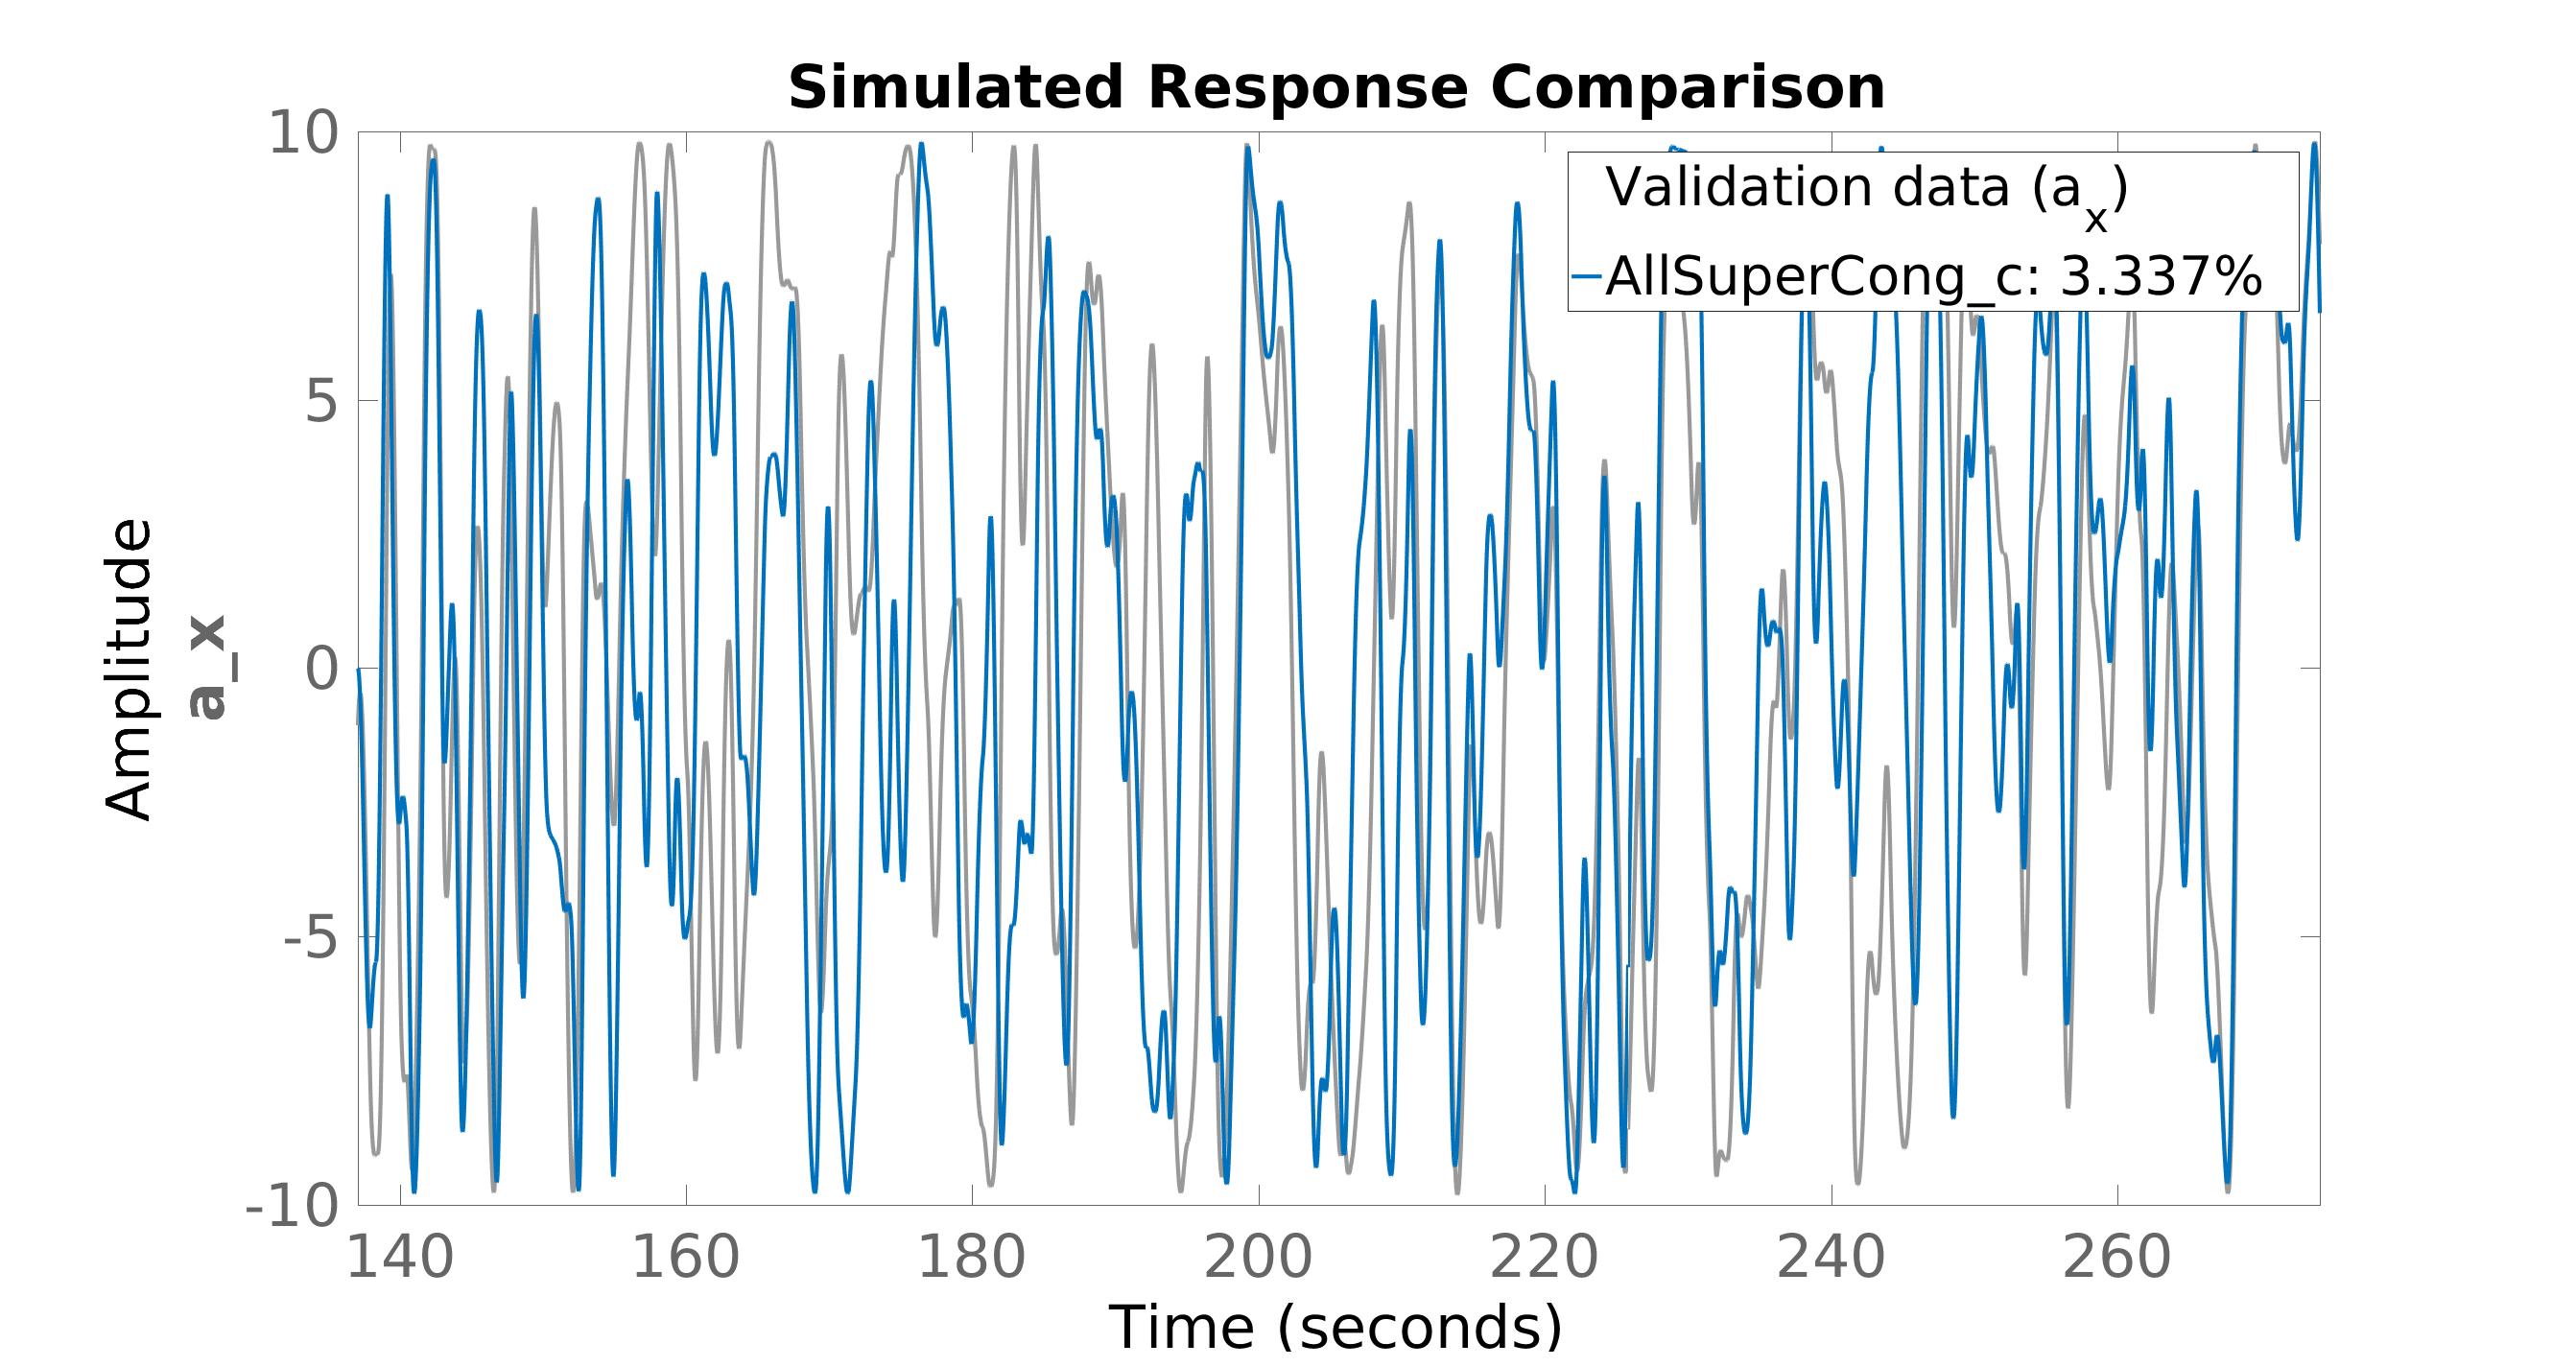
\includegraphics[width=0.4\textwidth]{linAccSimx}}
    \qquad
  \subfloat[][\label{fig:linAccSimy}Comparison of simulated linear acceleration in the \abbrROV's y-axis with simulated validation data.]{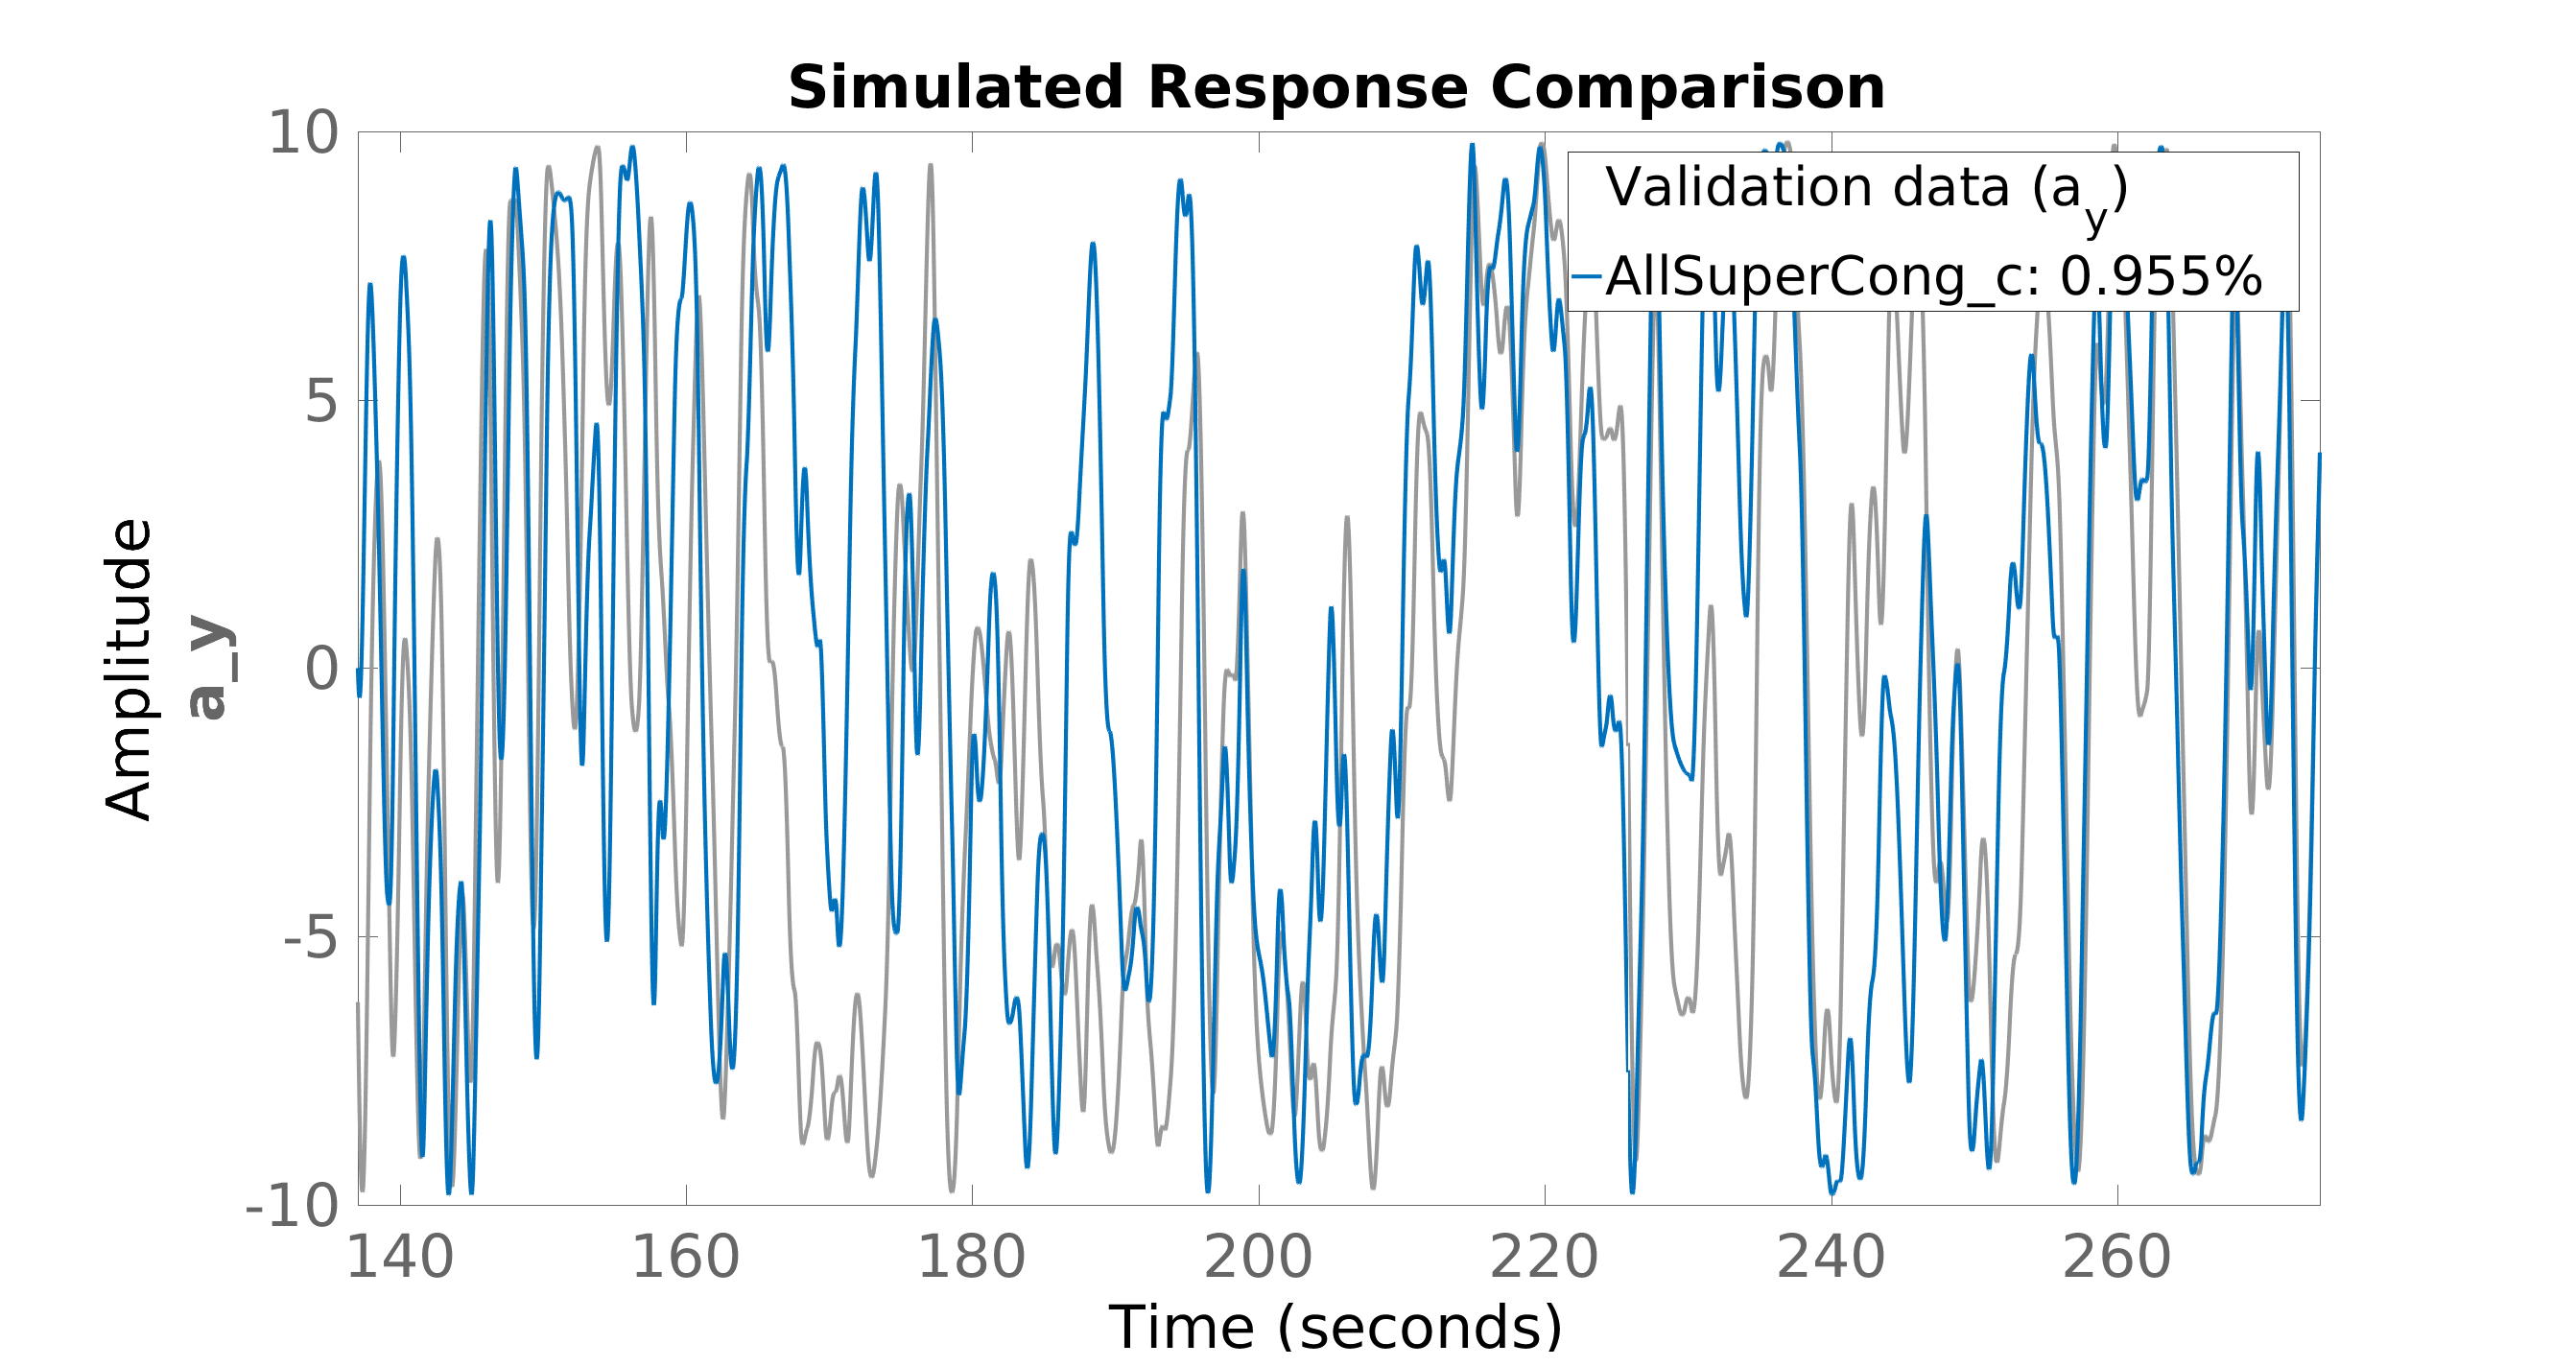
\includegraphics[width=0.4\textwidth]{linAccSimy}}
    \qquad
  \subfloat[][\label{fig:linAccSimz}Comparison of simulated linear acceleration  in the \abbrROV's z-axis with simulated validation data.]{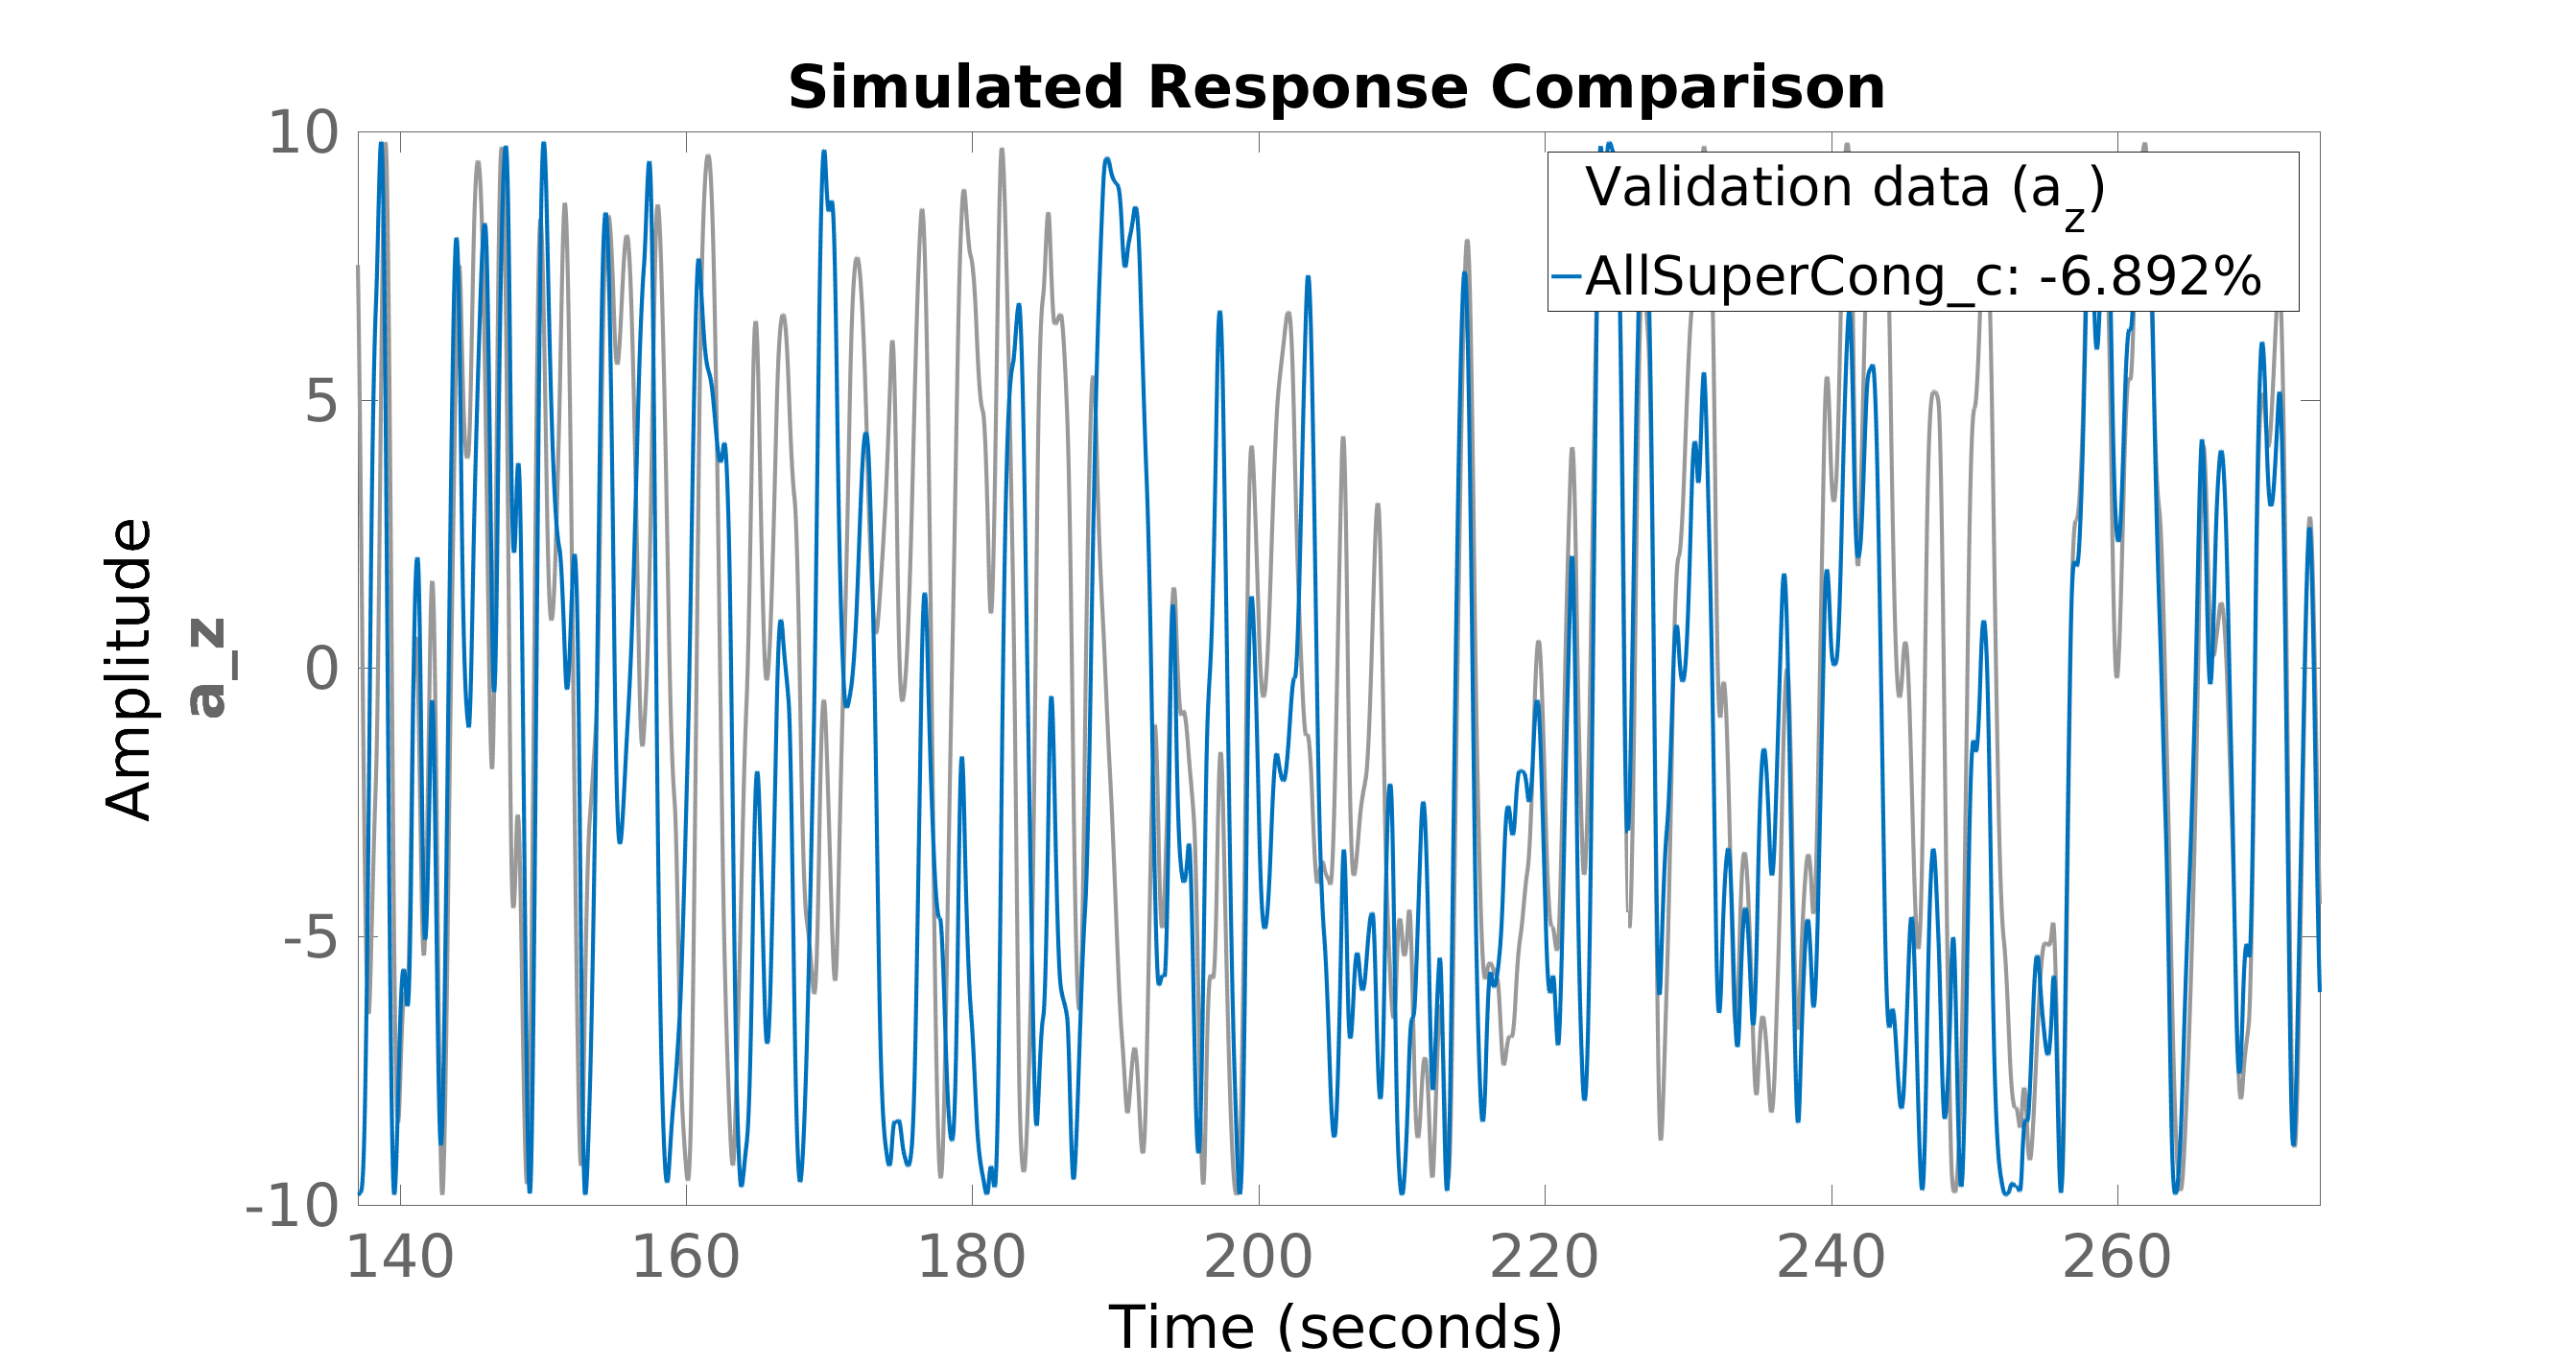
\includegraphics[width=0.4\textwidth]{linAccSimz}}
  \caption{\label{fig:angVelSim}%
    Comparison between simulated validation data (grey) and the simulated response from the estimated model(blue). The fit for the model in each state is stated in each plot. The validation data has been generated using the initial parameters used in the parameter estimation. The poor initial state estimate results in that the estimated parameters diverge from their true values.}
\end{figure}

Since data had been collected with Euler angles instead of quaternions and no simple way of estimating the initial state of the quaternions was thought of, a Kalman smoother as described in \citet{Wallin} was used introduced. The magnetometer was also added as a output, in the Kalman smoother, to further reduce the uncertainty of the initial quaternions. It is therefore recommended that when using quaternions during parameter estimation, that attitude data on quaternion form is logged so that the initial quaternions can easily be obtained. 

A problem that was consistent in all early estimations was a low fit value in $p$. Several adjustments were attempted in order to fix this issue and it was later found that the effect in $p$ of thruster 6 was minimal. A later test showed that thruster 6 only effected $p$ when it was quickly actuated. If the sixth thrusters power was incremented slowly an initial response in $p$ was noted before it settled at zero again. \todo{Add picture of this phenomenon}. This might be because of unmodelled translational dynamics of the \abbrROV meaning that the dynamics in $y$ may be coupled with $r$.

When deciding on which parameters to use for controller design, the choice was based solely on the fit of the simulated output had against validation data. The reasoning behind this being quite simple, the better the fit against validation data the less robust the controllers would have to be.



%%%%%%%%%%%%%%%%%%%%%%%%%%%%%%%%%%%%%%%%%%%%%%%%%%%%%%%%%%%
%\section{Decoupling the Model} \index{Decoupling}
% From \eqref{eq:WithoutTranslation} it can be seen that $r$ is not affected by the same thrusters as $p$ and $q$. Thus the $r$ model's parameters were initially estimated by themselves while the parameters in the $p$ and $q$ models were estimated together. 
%
%The estimation of the attitude model structure was divided into three estimation steps.
%
%The separately estimated parameters were then used as starting values for a complete attitude model parameter estimation, \eqref{eq:WithoutTranslation}. The reduced models for $r$, $p$ and $q$ that were used during initial estimation were
%
%The simplification could be done since excitation in the states not used in a particular estimation were kept at a minimum during data collection. Thus the coupled terms in each equation were approximated to be zero.

%%%%%%%%%%%%%%%%%%%%%%%%%%%%%%%%%%%%%%%%%%%%%%%%%%%%%%%%%%%
%\section{Parameter Estimation from Angular Velocities} \label{sec:estimation_angular}
%The estimated Euler angles from the sensor fusion model described in \Sectionref{sec:simple_model} did not follow the kinematic relation described in \Sectionref{sec:kinematics} which can be seen in \Figureref{fig:integratedAngleVelocities}. This also meant that the angles were unfit for use in as outputs in the parameter estimation since the angle estimates will not describe the system well since the estimates include the \abbrEKF's dynamics. The parameters were instead estimated using the angular velocities from the gyroscope as outputs an with the estimated euler angles as inputs. The model structure in which the parameters were estimated was thus \index{model structure}
%\begin{equation}
%\etaVectordot = f(\nuVector, \hat{\etaVector}, \tauVector),
%\end{equation}
%and
%\begin{equation}
%\boldsymbol{y} = \nuVector
%\end{equation}
%where $\hat{\etaVector}$ contains the estimated Euler angles from the sensor fusion.
%
%
%
%To get an initial estimate on the parameters in the yaw dynamics the reduced model parameters in \eqref{eq:r_dot_decouple}
%were estimated using data collected from a test that mainly excited the \abbrROV in $r$ which can be seen in \Figureref{r_rTest}.
%
%Since the dynamics in $p$ and $q$ are coupled \eqref{eq:pq_dot_decouple1} and \eqref{eq:pq_dot_decouple2} needed to be estimated at the same time. The cross terms in $r$ was assumed to be zero since the \abbrROV was mainly excited in $p$ and $q$ during collection of the used estimation data which can be seen in \Figureref{p_qTest}.
%
%The initial estimates of the parameters in \eqref{eq:pq_dot_decouple1} and \eqref{eq:r_dot_decouple} were used as initial estimates of the parameters in \eqref{eq:WithoutTranslation}. Due to observational problems the reparametrisation $A_p = \Ix - \Kpdot$, $B_q = \Iy - \Mqdot$ and $C_r = \Iz - \Nrdot$ was introduced. The fit can be seen in \Figureref{fig:velocityCompareCong} where the reparameterisation has been used.
%\index{Reduced model structure}
%
%%%%%%%%%%%%%%%%%%%%%%%%%%%%%%%%%%%%%%%%%%%%%%%%%%%%%%%%%%%%
%\section{Parameter Estimation from Angular Velocities and Linear Accelerations} \label{sec:angLinEstim}
%The parameters were also estimated using the angular velocities and the linear accelerations as outputs. This was done to avoid modelling the low-pass filtering effects in the sensor fusion described in \Chapterref{cha:sensor_fusion}. The model structure was modified to use quaternions instead of euler angles. Using quaternions in the model \eqref{eq:p_dotWithoutTranslation} - \eqref{eq:r_dotWithoutTranslation} with the reparameterision from \Sectionref{sec:estimation_angular} gave the model structure \todo{move model def to model chapter}
%\begin{multline}
%\pdot = \frac{\thrusterfun{1} \distance{y}{1} - \thrusterfun{2} \distance{y}{2} + \thrusterfun{6} \distance{z}{6}}{A_p} + \frac{B z_B (2 \quatII \quatIII + 2 \quatI \quatO)}{A_p} + \\ \frac{p (\Kp + \Kpabsp \abs{p})}{A_p} + \frac{q r (B_q - C_r)}{A_p},
%\end{multline}
%\begin{multline}
%\qdot = \frac{\thrusterfun{1} \distance{x}{1} + \thrusterfun{2} \distance{x}{2} - \thrusterfun{5} \distance{x}{5}}{B_q} - \frac{B z_B (2 \quatI \quatIII - 2 \quatII \quatO)}{B_q} + \\ \frac{q (\Mq + \Mqabsq \abs{q})}{B_q} - \frac{p r (A_p - C_r)}{B_q}
%\end{multline}
%and
%\begin{multline}
%\rdot = \frac{\thrusterfun{3} \distance{y}{3} - \thrusterfun{4} \distance{y}{4}}{C_r} + \frac{r (\Nr + \Nrabsr \abs{r}}{C_r} + \frac{p q (A_p  - B_q)}{C_r}
%\end{multline}
%
%Thus the model structure in which the parameters was estimated became \index{model structure}
%\begin{equation}
%\etaVectordot = J(\etaVector) \nuVector,
%\end{equation}
%\begin{equation}
%\dot{\nuVector} =  f(\etaVector, \nuVector, \tauVector)
%\end{equation}
%with 
%\begin{equation}
%\boldsymbol{y} = \begin{pmatrix}
%\etaVector \\
%\boldsymbol{a}
%\end{pmatrix}
%\end{equation}
%where $\boldsymbol{a}$ are the linear accelerations in the \abbrROV frame. 
%
%The fit of the model compared to validation data can be seen in \Figureref{fig:angVelCompare}. To properly estimate the parameters the initial states had to be well estimated. The importance of a correct initial state estimate can be seen in \Figureref{fig:angVelSim}. Here the estimator was fed simulated data and was initialised with the true parameter values but had to estimate the starting state.   The estimated starting state was not well estimated, which in turn led to the parameters diverging from the true parameters and a low fit. A Kalman smoother as described in \citet{Wallin} was used introduced in order to alleviate this problem. During initial state estimation using the Kalman smoother the magnetometer was added as a output to reduce the uncertainty of the initial quaternions.
%
%
%To handle noisy signals an error threshold was introduced. An error threshold means that after a breakpoint the cost function becomes linear instead of quadratic. This makes the parameter estimation less sensitive to outliers. To reduce the impact of the noise even further the used weight matrix in the cost function was the inverse of the estimated noise covariance. 

%%%%%%%%%%%%%%%%%%%%%%%%%%%%%%%%%%%%%%%%%%%%%%%%%%%%%%%%%%%%
\section{Estimated Parameters}\todo{Update Parameters, lz6 = 0}
\Tableref{tab:parameterConstants} shows the know and measured parameters used in the \abbrROV. The estimated parameters used in the \abbrROV model are shown in \Tableref{tab:parameterEstimation}.

\begin{table}[tbp]
  \centering
  \caption{\label{tab:parameterConstants}%
    The known parameters used in the \abbrROV model.}
  \begin{tabular}{l l p{0.7\linewidth}}
    \toprule%
    \textbf{Notation}   & \textbf{Value} & \textbf{Description} \\
    \otoprule%
    $m$                 & 6.621 \kilogram                    & Mass of the \abbrROV. \\            
    $g$                 & 9.82  \meter\per\second\squared    & Gravity acceleration.\\   
    $\rho$              & 1000  \kilogram\per\meter\cubed    & Density of water.\\       
    
    $\distance{x}{1}$   & 0.16 \meter & Distance from \abbrCG to thruster 1 in $\xPosition$-direction.\\
    $\distance{y}{1}$   & 0.11 \meter & Distance from \abbrCG to thruster 1 in $\yPosition$-direction.\\
    $\distance{y}{2}$   & 0.11 \meter & Distance from \abbrCG to thruster 2 in $\yPosition$-direction.\\
    $\distance{x}{2}$   & 0.16 \meter & Distance from \abbrCG to thruster 2 in $\xPosition$-direction.\\
    $\distance{y}{3}$   & 0.11 \meter & Distance from \abbrCG to thruster 3 in $\yPosition$-direction.\\
    $\distance{x}{5}$   & 0.20 \meter & Distance from \abbrCG to thruster 5 in $\xPosition$-direction.\\
    $\distance{y}{4}$   & 0.11 \meter & Distance from \abbrCG to thruster 4 in $\yPosition$-direction.\\
    $\distance{z}{6}$   & 0.11 \meter & Distance from \abbrCG to thruster 6 in $\zPosition$-direction.\\
    \bottomrule%
  \end{tabular}
\end{table}

\begin{table}[tbp]
  \centering
  \caption{\label{tab:parameterEstimation}%
    The estimated parameters used in the \abbrROV model.}
  \begin{tabular}{l l p{0.7\linewidth}}
    \toprule%
    \textbf{Notation}   & \textbf{Value} & \textbf{Description} \\
    \otoprule%   
    % Parameters that will be estimated
	$z_B$               & -0.0308 \meter                                      & Distance from \abbrCG to \abbrCB.\\
    $\Kp$               & -1.1082 \kilogram\usk\meter\squared                 & Linear damping coefficient due to rotation in water about the $\xPosition$-axis.\\
    $\Kpabsp$           & -0.3450 \kilogram\usk\meter\squared                 & Quadratic damping coefficient due to rotation in water about the $\xPosition$-axis.\\
    $\Mq$               & -1.2385 \kilogram\usk\meter\squared                 & Linear damping coefficient due to rotation in water about the $\yPosition$-axis.\\
    $\Mqabsq$           & -0.1111 \kilogram\usk\meter\squared                 & Quadratic damping coefficient due to rotation in water about the $\yPosition$-axis.\\
    $\Nr$               & -1.5325 \kilogram\usk\meter\squared                 & Linear damping coefficient due to rotation in water about the $\zPosition$-axis.\\
    $\Nrabsr$           & -1.3977 \kilogram\usk\meter\squared                 & Quadratic damping coefficient due to rotation in water about the $\zPosition$-axis.\\
    $A_p$               & 0.9625  \kilogram\usk\meter\squared                 & Inertia around the $\xPosition$-axis and increased inertia around the $\xPosition$-axis.\\
    $B_q$               & 0.7108  \kilogram\usk\meter\squared                 & Inertia around the $\yPosition$-axis and increased inertia around the $\yPosition$-axis.\\
    $C_r$               & 1.2649  \kilogram\usk\meter\squared                 & Inertia around the $\zPosition$-axis and increased inertia around the $\zPosition$-axis.\\
    \bottomrule%
  \end{tabular}
\end{table}
\chapter{Controlling the ROV} \label{cha:controller} \index{Open-Loop Control} \index{Controller} \index{Exact Linearisation}
Automatic control is way of regulating a process without direct human interaction. The complexity can vary from decentralised proportional, integral and derivative controllers (\abbrPID:s) to more advanced model-based control methods, such as model predictive control (\abbrMPC). 

There are two main concepts of control, open-loop and feedback control. An open-loop controller is a controller that computes its output based on a model of the system and sometimes the current states. A disadvantage of open-loop controllers is that they require exact knowledge of the controlled system \citep{reglerteknik}. \Figureref{fig:control_system_open} illustrates the open-loop control scheme used in the \abbrROV. 

A feedback controller is a controller that uses measurements of the states in a system to correct its actions. One such method is error-controlled regulation, where the difference between the desired value, setpoint, of a state and its actual value is used for control. The feedback control scheme used in the \abbrROV can be seen in \Figureref{fig:control_system}. 

Similarly to an open-loop controller, a feedback controller can use a model of the system. Using a model of the controlled system in the control structure can produce better performance and compensate for unwanted effects such as non-linearities. Compensating for non-linearities is desired due to the fact that a lot of control principles are based on linear systems \citep{reglerteori}. 

\begin{figure}
	\centering
		\begin{tikzpicture}[auto, thick, node distance=2cm,>=latex',
			 block/.style  = {draw, rectangle,minimum height=3em, minimum width=6em},
			 sum/.style    = {draw, circle, inner sep=0pt, text width=4mm,align=center, node distance=1cm},
			 input/.style  = {coordinate},
			 output/.style = {coordinate},
			 pinstyle/.style = {pin edge={to-,thin,black}}]
			 
		    \node [input, name=input] {};
		    \node [block, right of=input, node distance=3cm] (controller) {F};
		    \node [block, right of=controller, node distance=3cm] (system) {\abbrROV};
		
		    \draw [->] (controller) -- node[name=u] {$u$} (system);
		    \node [output, right of=system] (output) {};
		
		    \draw [draw,->] (input) -- node {$u_{\text{control}}$} (controller);
		    \draw [->] (system) -- node [name=y] {$y$}(output);
		\end{tikzpicture}
	\caption{The open-loop control scheme used in the \abbrROV. The control block F can be any type of open-loop control. Notice that this is an ideal case were no disturbances affect the system.}
	\label{fig:control_system_open}
\end{figure}

\begin{figure}
	\centering
		\begin{tikzpicture}[auto, thick, node distance=2cm,>=latex',
			 block/.style  = {draw, rectangle,minimum height=3em, minimum width=6em},
			 sum/.style    = {draw, circle, inner sep=0pt, text width=4mm,align=center, node distance=1cm},
			 input/.style  = {coordinate},
			 output/.style = {coordinate},
			 pinstyle/.style = {pin edge={to-,thin,black}}]
			 
		    \node [input, name=input] {};
		    \node [sum, right of=input] (sum) {+};
		    \node [block, right of=sum] (controller) {F};
		    \node [block, right of=controller, node distance=3cm] (system) {\abbrROV};
		
		    \draw [->] (controller) -- node[name=u] {$u$} (system);
		    \node [output, right of=system] (output) {};
		    \node [block, below of=u] (sensorfusion) {Observer};
		
		    \draw [draw,->] (input) -- node {$x_{\text{ref}}$} (sum);
		    \draw [->] (sum) -- node {$e$} (controller);
		    \draw [->] (system) -- node [name=y] {$y$}(output);
		    \draw [->] (y) |- (sensorfusion);
		    \draw [->] (sensorfusion) -| node[pos=0.99] {$-$} 
		        node [near end] {$\hat{x}$} (sum);
		\end{tikzpicture}
	\caption{The feedback control scheme used in the \abbrROV. The controller F can be any of the controllers discussed in this chapter. The observer in the \abbrROV is the sensor fusion described in \Chapterref{cha:sensor_fusion}. Notice that this is an ideal case were no disturbances effect the system.}
	\label{fig:control_system}
\end{figure}


%%%%%%%%%%%%%%%%%%%%%%%%%%%%%%%%%%%%%%%
\section{Open-Loop Control} \label{sec:openloop} \index{Open-Loop Control} \index{thrust allocation} \index{thruster geometry}
The open loop control of the \abbrROV consists of an static thrust allocation matrix which is
\begin{equation}
    \thrusterGeometryOnes[*] = \thrusterGeometryOnes[T](\thrusterGeometryOnes \thrusterGeometryOnes[T])^{-1}
\end{equation}
where $\thrusterGeometryOnes$ describes how the actuators effect the \abbrROV \citep{thrustallocation}. The thrust geometry matrix $\thrusterGeometryOnes$ has been derived from the thrust matrix $\thrusterGeometry$ and became 
\begin{equation*}
    \thrusterGeometryOnes = 
    \begin{bmatrix}
    0  & 0  & 1 & 1  &  0 &  0 \\
    0  & 0  & 0 & 0  &  0 & -1 \\
    -1 & -1 & 0 & 0  & -1 &  0 \\
    1  & -1 & 0 & 0  &  0 &  0 \\
    1  & 1  & 0 & 0  & -1 &  0 \\
    0  & 0  & 1 & -1 &  0 &  0 \\
    \end{bmatrix}
\end{equation*}
and thus $\thrusterGeometryOnes[*]$ is given by
\begin{equation}
\thrusterGeometryOnes= \begin{bmatrix}
0 & 0 & -0.25 & 0.5 & 0.25 & 0 \\
0 & 0 & -0.25 & -0.5 & 0.25 & 0 \\
0.5 & 0 & 0 & 0 & 0 & 0.5 \\
0.5 & 0 & 0 & 0 & 0 & -0.5 \\
0 & 0 & -0.5 & 0 & -0.5 & 0 \\
0 & -1 & 0 & 0 & 0 & 0 \\
\end{bmatrix}
\end{equation}
The static thrust allocation matrix $\thrusterGeometryOnes[*]$ is the pseudo inverse of the thrust geometry matrix $\thrusterGeometryOnes$. An approximately decoupled control is achieved when the static thrust allocation matrix is used and thus can the \abbrROV be controlled better without using any controllers. \Figureref{fig:open_control} illustrates how the control signals are allocated to the different thrusters when given an control input.

\begin{figure}
    \centering
    \begin{tikzpicture}[auto, thick, node distance=3cm, >=latex',%
        block/.style    = {draw, thick, rectangle, minimum height = 3em,%
        minimum width = 3em},%
      sum/.style      = {draw, circle, node distance = 2cm},% 
      input/.style    = {coordinate},%
      output/.style   = {coordinate} %
    ]
    \draw
    	% Drawing the blocks of first filter :
    	node at (0,0)[input, name=input1] (input1) {}
    	node [block, right of=input1] (inte1) {\thrusterGeometryOnes[*]}
    	node [output, right of=inte1] (output1) {};
        % Joining blocks. 
        % Commands \draw with options like [->] must be written individually
    	\draw[->](input1) -- node {$u_{\text{control}}$}(inte1);
     	\draw[->](inte1) -- node {$u$} (output1);
    \end{tikzpicture}
    \caption{The open-loop control allocate control signals by the thrust allocation matrix $\thrusterGeometryOnes[*]$. The static thrust allocation matrix gives an approximately decoupled control.}
    \label{fig:open_control}
\end{figure}

%%%%%%%%%%%%%%%%%%%%%%%%%%%%%%%%%%%%%%%%
\section{Exact Linearisation}
To compensate for the non-linearities in a system using a non-linear control law is called exact linearisation. Doing this makes the system linear from a input-output perspective \citep{reglerteori}. Using the model structure from \Chapterref{cha:modelling} and the estimated parameters from \Chapterref{cha:parameterEstimation} a non-linear control law was created 
\begin{equation}\label{eq:exactLin}
\tauVector_{\text{Lin}} = G^{-1}(\hat{\etaVector}_{2},\hat{\nuVector}_{2},\accVector^{\text{b}}) = \inertia \accVector^{\text{b}} + \damping(\hat{\nuVector}_{2})\hat{\nuVector}_{2} + \coriolis(\hat{\nuVector}_{2})\hat{\nuVector}_{2} + \gravity(\hat{\etaVector}_{2})
\end{equation}
where $\accVector^b$ is the desired angular acceleration in the body-fixed frame and $\tauVector_{\text{Lin}}$ is the estimated thrust needed to achieve the desired acceleration.
The desired control signal $\boldsymbol{u}_{\text{Lin}}$ was then chosen using 
\begin{equation}\label{eq:linControlSignal}
\boldsymbol{u}_{\text{Lin}} = \boldsymbol{T}^{-1}f^{-1}(\bar{\tauVector}_{\text{Lin}})
\end{equation} where $f$ is the look-up table from control signal to thrust defined in \appref{app:thrustmapping}, $T$ is the geometry matrix defined in \eqref{eq:actuatorGeometry} and $\bar{\tauVector}_{\text{Lin}}=[0~0~0~\tauVector_{\text{Lin}}^T]^T$.
In an ideal case, where the model is exact, using the non-linear control law \eqref{eq:exactLin} would produce the system
\begin{equation}\label{eq:exactLinSys}
\nuVectorAngdot = \accVector^b
\end{equation} 
where $\accVector^b$ could be chosen using any desired control method \citep[p.451]{fossen2011}.

%%%%%%%%%%%%%%%%%%%%%%%%%%%%%%%%%%%%%%%%
\section{Attitude Controller} \index{PID@\abbrPID!abbreviation} \index{Attitude Controller}
An attitude controller was also implemented on the \abbrROV. The controller was chosen as \abbrPID-controller utilising exact linearisation \eqref{eq:exactLin}.
Since \eqref{eq:exactLin} aimed to linearise the angular accelerations in the body-fixed frame and not the angular accelerations in the global coordinate system, an extra control law was needed.
Choosing 
\begin{equation}\label{eq:anLaw}
\accVector^b =L(\accVector^n,\hat{\eulerAngles},\hat{\nuVector}_2)=\boldsymbol{T}^{-1}_\theta(\hat{\eulerAngles})(\accVector^n - \dot{\boldsymbol{T}}_\theta(\hat{\eulerAngles})\hat{\nuVector}_2)\\
\end{equation} where $\accVector^n$ is the desired angular acceleration in the global-frame. This gives the following linear system \begin{equation}
\ddot{\boldsymbol{\eta}}_2=\accVector^n 
\end{equation}
Defining the control error as
\begin{equation}
\etaTildeAng = \hat{\etaVector}_2 - \etaVectorAng[,_{\text{ref}}] 
\end{equation}
$\accVector^n$ could be chosen using the following feedback 
\begin{equation}\label{eq:attitudeFeedback}
\accVector^n=-K_{\text{p}} \etaTildeAng - K_{\text{i}}\int \! \etaTildeAng \, \mathrm{d}t - K_{\text{d}} \etaTildeAngdot
\end{equation}
where $K_{\text{p}}$, $K_{\text{i}}$ and $K_{\text{d}}$ are positive definite design matrices \citep[p. 453]{fossen2011}. 
Using \eqref{eq:kinematicsticsEuler} and the assumption that $\etaVectorAng[,_{\text{ref}}]$ is piece-wise constant, the derivative of the attitude error could be defined as 
\begin{equation}\label{eq:etaTildeAngDot}
\etaTildeAngdot = \boldsymbol{T}_\theta(\hat{\boldsymbol{\Theta}})\hat{\nuVector}_{2}
\end{equation}
Combining \eqref{eq:etaTildeAngDot} with \eqref{eq:attitudeFeedback} gives the feedback
\begin{equation}
\accVector^n=-K_{\text{p}} \etaTildeAng - K_{\text{i}}\int \! \etaTildeAng \, \mathrm{d}t - K_{\text{d}} \boldsymbol{T}_\theta(\hat{\boldsymbol{\Theta}})\hat{\nuVector}_{2}
\end{equation}

%This gives the \abbrPID attitude controller
%\begin{equation}
%	\accVector^b = \begin{bmatrix} 
%	\zeroCol{3} \\
%	\boldsymbol{T}^{-1}_\theta(\eulerAngles)(-K_{\text{p}} \etaTildeAng - K_{\text{i}}\int \! \etaTildeAng \, \mathrm{d}t - K_{\text{d}} \etaTildeAngdot - \dot{\boldsymbol{T}}_\theta(\eulerAngles) \nuVectorAng)
%	\end{bmatrix}
%\end{equation}
%where $K_{\text{p}}$, $K_{\text{i}}$ and $K_{\text{d}}$ are positive definite design matrices \citep[p. 453]{fossen2011}. 
The attitude controller was also combined with an open-loop control of the linear velocities
\begin{equation}
	u_{\etaVector} = \boldsymbol{T}^{-1}f^{-1}(G^{-1}(\hat{\etaVector}_2,\hat{\nuVector}_2,L(\accVector^n,\hat{\eulerAngles},\hat{\nuVector}_2))) + \thrusterGeometryOnes[*] \begin{bmatrix} \nuVector_{1,\text{ref}} \\ \zeroCol{3} \end{bmatrix}
\end{equation}
or
\begin{equation}
	u_{\etaVector} = \boldsymbol{T}^{-1}f^{-1}(L(\accVector^n,\hat{\eulerAngles},\hat{\nuVector}_2)) + \thrusterGeometryOnes[*] \begin{bmatrix} \nuVector_{1,\text{ref}} \\ \zeroCol{3} \end{bmatrix}
\end{equation}
without the exact linearisation. This was implemented to allow the user to steer the \abbrROV while the controller unsures that the \abbrROV holds a given attitude. An illustration of how the attitude controller with open-loop control is implemented can be seen in \Figureref{fig:attitudecontroller}.

\begin{figure}
	\centering
	\begin{tikzpicture}[auto, thick, node distance=2cm, >=latex',%
        block/.style  = {draw, thick, rectangle, minimum height = 1cm,%
                           minimum width = 3em},%
        PID/.style    = {draw, thick, rectangle, minimum height = 1cm,%
                         minimum width = 0.6cm},%
        sum/.style    = {draw, circle,inner sep=0pt, text width=4mm,align=center,node distance = 1cm},%
        mux/.style    = {draw, thick, rectangle, minimum width=0.3cm,%
                        minimum height = 2cm ,fill= black!100,%
                        node distance=1cm},
        input/.style    = {coordinate},%
        output/.style   = {coordinate} %
    ]
   		\draw node at (0,0) [input] (vel_input) {};
   		\draw node [input,below of=vel_input, node distance=3cm] (ang_input) {};
   		\draw node[PID, right of=ang_input, node distance=1cm] (pid) {$\abbrPID$};
   		\draw node[block, right of=pid, node distance=1.3cm] (L) {$L(\cdot)$};
   		
   		%from input to pid
   		\draw[->] (ang_input) -- node[align=center, below] {$\etaTildeAng$} ($(pid.west)$);
   		\draw[->] (pid.east) -- (L.west);
   		\draw (L.east) -- ++(0.5,0) node[](switch){};
   		
   		%from pid to switch and making the switch 
   		\draw (L.east) ++(2,0.5) node[](switchup){};
   		\draw (L.east) ++(2,-0.5) node[block, name=exactlin] {$G^{-1}(\cdot)$};
   		\draw (L.east) ++(0.8,0.5) -| (switchup);
   		\draw (L.east) ++(0.8,-0.5) -| (exactlin.west);
   		\draw (L.east) ++(0.5,0) -- ++(0.3,0.5);
   		\draw[->] (L.east) ++(0.65,0.25) arc (30:-30:0.6);     		
   		
   		%Merge the switch  		
   		\draw (L.east) ++(3,0) node[coordinate](merge){};
   		\draw (switchup) -| (merge);
   		\draw (exactlin) -| (merge);
   		
   		%Input to thrust
   		\draw node[block, right of=vel_input] (thrust) {$\thrusterGeometryOnes[*]$};
   		\draw[->] (vel_input) -- node[align=center, below] {$\nuVectorLin[,\text{ref}]$} (thrust.west);
   		
   		
   		%To sum
   		\draw (thrust.east) ++(4,0) node[sum, name=sum] {$+$};
		\draw[->] (thrust.east) -- node[align=center, below] {$u_{\nuVectorLin}$} (sum.west);
		%From exact lin to sum
   		\draw node[block, below of=sum, node distance=1.5cm] (rotate) {$T^{-1}$};
   		\draw node[block, right of=merge, node distance=1cm] (inter) {$f^{-1}(\cdot)$};
   		\draw[->] (rotate.north) -- node[align=center, right] {$u_{\etaVectorAng}$} (sum.south);
   		\draw[->] (inter.north) -| (rotate.south);
   		\draw[->] (merge) -- (inter.west);   		   		
   		% From sum to output
   		\draw node [output, right of=sum, node distance=2cm] (output) {};
    		\draw[->] (sum.east) -- node[align=center, below] {$u$} (output);	
	\end{tikzpicture}
    \caption{The linear velocities are controlled in the same way as in \Sectionref{sec:openloop}. However, the attitude are controlled via an \abbrPID and exact linearisation can be enabled.} 
    \label{fig:attitudecontroller}
\end{figure}

%%%%%%%%%%%%%%%%%%%%%%%%%%%%%%%%%%%%%%%%
\section{Angular Velocities Controller} \index{Angular Velocities Controller} \index{PI@\abbrPI!abbreviation}
An angular velocity controller was also implemented using the exact linearisation \eqref{eq:exactLin}.
Since no transformation is needed in order to control angular velocities in the body-fixed frame
$\accVector^b$ can be chosen using the following \abbrPI feedback 
\begin{equation}
	\accVector^b =-K_{\text{p}} \nuTildeAng - K_{\text{i}}\int \! \nuTildeAng \, \mathrm{d}t
\end{equation}
where $K_{\text{p}}$ and $K_{\text{i}}^b$ are positive definite design matrices and 
\begin{equation}
\nuTildeAng = \hat{\nuVector}_2 - \nuVectorAng[,_{\text{ref}}]
\end{equation} \citep[p. 453]{fossen2011}.

The \abbrPI controller for the angular velocities controller was also expanded with a open-loop control solution for the linear velocities
\begin{equation}
	u_{\nuVectorAng} = \boldsymbol{T}^{-1}f^{-1}(G^{-1}(\hat{\etaVector}_2,\hat{\nuVector}_2,\accVector^b)) + \thrusterGeometryOnes[*] \begin{bmatrix}\nuVector_{1,\text{ref}} \\ \zeroCol{3} \end{bmatrix}	
\end{equation}
or alternatively 
\begin{equation}
	u_{\nuVectorAng} = \boldsymbol{T}^{-1}f^{-1}(\accVector^b) + \thrusterGeometryOnes[*] \begin{bmatrix} \nuVector_{1,\text{ref}} \\ \zeroCol{3} \end{bmatrix}
\end{equation}
if the exact linearisation is removed. \Figureref{fig:ratecontroller} illustrates how the angular velocity controller is implemented in conjunction with the open-loop control of the linear velocities.
\begin{figure}
	\centering
	\begin{tikzpicture}[auto, thick, node distance=2cm, >=latex',%
        block/.style  = {draw, thick, rectangle, minimum height = 1cm,%
                           minimum width = 3em},%
        PID/.style    = {draw, thick, rectangle, minimum height = 1cm,%
                         minimum width = 0.6cm},%
        sum/.style    = {draw, circle,inner sep=0pt, text width=4mm,align=center,node distance = 1cm},%
        mux/.style    = {draw, thick, rectangle, minimum width=0.3cm,%
                        minimum height = 2cm ,fill= black!100,%
                        node distance=1cm},
        input/.style    = {coordinate},%
        output/.style   = {coordinate} %
    ]
   		\draw node at (0,0) [input] (vel_input) {};
   		\draw node [input,below of=vel_input, node distance=3cm] (ang_input) {};
   		\draw node[PID, right of=ang_input] (pid) {$\abbrPI$};
   		
   		%from input to pid
   		\draw[->] (ang_input) -- node[align=center, below] {$\nuTildeAng$} ($(pid.west)$);
   		\draw (pid.east) -- ++(0.5,0) node[](switch){};
   		
   		%from pid to switch and making the switch 
   		\draw (pid.east) ++(2,0.5) node[](switchup){};
   		\draw (pid.east) ++(2,-0.5) node[block, name=exactlin] {$G^{-1}(\cdot)$};
   		\draw (pid.east) ++(0.8,0.5) -| (switchup);
   		\draw (pid.east) ++(0.8,-0.5) -| (exactlin.west);
   		\draw (pid.east) ++(0.5,0) -- ++(0.3,0.5);
   		\draw[->] (pid.east) ++(0.65,0.25) arc (30:-30:0.6);     		
   		
   		%Merge the switch  		
   		\draw (pid.east) ++(3,0) node[coordinate](merge){};
   		\draw (switchup) -| (merge);
   		\draw (exactlin) -| (merge);
   		
   		%Input to thrust
   		\draw node[block, right of=vel_input] (thrust) {$\thrusterGeometryOnes[*]$};
   		\draw[->] (vel_input) -- node[align=center, below] {$\nuVectorLin[,\text{ref}]$} (thrust.west);
   		
   		%To sum
   		\draw (thrust.east) ++(4,0) node[sum, name=sum] {$+$};
		\draw[->] (thrust.east) -- node[align=center, below] {$u_{\nuVectorLin}$} (sum.west);
		%From exact lin to sum
   		\draw node[block, below of=sum, node distance=1.5cm] (rotate) {$T^{-1}$};
   		\draw node[block, right of=merge, node distance=1.5cm] (inter) {$f^{-1}(\cdot)$};
   		\draw[->] (rotate.north) -- node[align=center, right] {$u_{\etaVectorAng}$} (sum.south);
   		\draw[->] (inter.north) -| (rotate.south);
   		\draw[->] (merge) -- (inter.west);
   		% From sum to output
   		\draw node [output, right of=sum, node distance=2cm] (output) {};
    		\draw[->] (sum.east) -- node[align=center, below] {$u$} (output);	  
	\end{tikzpicture}
    \caption{The linear velocities are controlled in the same way as in \Sectionref{sec:openloop}. However, the angular velocities are controlled via an \abbrPI and exact linearisation can be enabled.} 
    \label{fig:ratecontroller}
\end{figure}

%%%%%%%%%%%%%%%%%%%%%%%%%%%%%%%%%%%%%%%%
\section{Depth Controller} \index{Depth Controller} \index{PI@\abbrPI!abbreviation}
A \abbrPI-depth controller was also implemented on the \abbrROV. The depth controller was designed such that it could be used simultaneously with any other the aforementioned rate- and attitude controllers. 

If the error in depth $d$ is defined as 
\begin{equation}
\tilde{d} = d - d_{\text{ref}}
\end{equation}
then the \abbrPI depth controller can be defined as
\begin{equation}
u_{\zPosition} = \thrusterGeometryOnes[*]\begin{bmatrix} \boldsymbol{R}^n_b(\hat{\Theta})^T \begin{bmatrix}
0 \\
0 \\
- K_{\text{p}} \tilde{\zPosition} - K_{\text{i}}\int \! \tilde{\zPosition} \, \mathrm{d}t
\end{bmatrix} \\ \zeroCol{3}\end{bmatrix}
\end{equation}
where $K_{\text{p}}$ and $K_{\text{i}}$ are design parameters. The rotation matrix $\boldsymbol{R}^n_b(\hat{\Theta})^T$ is used to enable the depth controller to distribute control signals depending on the attitude of the \abbrROV. This enables the controller to regulate the depth regardless of the \abbrROV's attitude. The implementation of the depth controller can be seen in \Figureref{fig:depthcontroller}.


\begin{figure}
	\centering
	\begin{tikzpicture}[auto, thick, node distance=2cm, >=latex',%
        block/.style  = {draw, thick, rectangle, minimum height = 1cm,%
                           minimum width = 3em},%
        PID/.style    = {draw, thick, rectangle, minimum height = 1cm,%
                         minimum width = 0.6cm},%
        sum/.style    = {draw, circle,inner sep=0pt, text width=4mm,align=center,node distance = 1cm},%
        mux/.style    = {draw, thick, rectangle, minimum width=0.3cm,%
                        minimum height = 2cm ,fill= black!100,%
                        node distance=1cm},
        input/.style    = {coordinate},%
        output/.style   = {coordinate} %
    ]
   		\draw node at (0,0) [input] (vel_input) {};
		\draw node[input, below of=vel_input,node distance=2.5cm] (ang_input) {};
   		\draw node[PID, right of=ang_input] (pid) {$\abbrPI$};
   		
   		%from input to pid
   		\draw[->] (ang_input) -- node[align=center, below] {$\tilde{\zPosition}$} ($(pid.west)$);
   		\draw (pid.east) -- ++(0.5,0) node[](switch){};
   		
   		%from pid to switch and making the switch 
   		\draw (pid.east) ++(2,0) node[coordinate](switchup){};
  		\draw (pid.east) ++(1.2,0) -- (switchup);
   		\draw (pid.east) ++(0.5,0) -- ++(0.3,0.5);
   		\draw[->] (pid.east) ++(0.65,0.25) arc (30:0:0.6);     		
   		
   		%Merge the switch  		
   		%\draw (pid.east) ++(2,0) node[coordinate](merge){};
   		%\draw (switchup) -- (merge);
   		
   		%Input to thrust
   		\draw node[block, right of=vel_input] (controller) {F};
   		\draw[->] (vel_input) -- node[align=center, below] {$x_{\text{ref}}$} (controller.west);
   		
   		%To sum
   		\draw (controller.east) ++(4,0) node[sum, name=sum] {$+$};
		\draw[->] (controller.east) -- (sum.west);
		\draw node[block, right of=switchup,node distance=1cm] (rotate) {$\boldsymbol{R}^n_b(\hat{\Theta})^T$};
		\draw node[block, below of=sum,node distance=1.3cm] (thrust) {$\thrusterGeometryOnes[*]$};
		\draw[->] (switchup) -- (rotate.west); 
		\draw[->] (rotate.east) -| (thrust.south); 
   		\draw[->] (thrust.north) -- node[align=center, right] {$u_{\zPosition}$}  (sum.south);   		   		
   		% From sum to output
   		\draw node [output, right of=sum, node distance=2cm] (output) {};
    		\draw[->] (sum.east) -- node[align=center, right] {$u$} (output);
	\end{tikzpicture}
    \caption{The \abbrPI depth controller can be used when the open-loop control is engaged or when the other controllers are used. In this figure the F symbolises the chosen way of controlling the \abbrROV.} 
    \label{fig:depthcontroller}
\end{figure}

%%%%%%%%%%%%%%%%%%%%%%%%%%%%%%%%%%%%%%%%
\section{Benchmarking}
To be able to draw any conclusions about the performance of the controllers the following reference signals were used during tests
\begin{description}
\item[Constant] A constant reference was applied to all \abbrDOF. This reference signal was only used for trimming the controllers initially, thus will no results be presented except for the depth controller.

\item[Sine] A $\sin(\cdot)$ signal was applied to one \abbrDOF at the time and then to all \abbrDOF. Two $\sin$ signals with different amplitudes were used, amplitude $1$ and $0.5$. The used frequency was $0.5 \hertz$.

\item[Smooth step] A smooth step was applied to one \abbrDOF at the time and then to all \abbrDOF at the same time. The used smooth step was the same as in \citet[p. 192]{robotics}. The smooth step parameters were $q_{\text{0}} = 0$, $q_{\text{f}} = 1$, $t_{\text{s}} = 3$ ,$t_{\text{f}} = 15$ and $V = 1.5 (q_{\text{f}} - q_{\text{0}})/(t_{\text{f}} - t_{\text{s}}))$
\end{description}
for each controller separately. For each conducted test, except for depth tests, a simulated test was also performed. The \abbrROV model used during simulation used the parameters from \Sectionref{sec:parameterResults}. The exact linearisation, both in the simulator and the \abbrROV, used the parameters from \Sectionref{sec:parameterResults} with a scaling factor of 0.9 all parameters except for $z_B$ which was scaled by 0.5. In this Section a few representative test cases will be presented, several more tests were conducted and these can be seen in \Appref{app:controllerTestResults}. 
Tests were conducted with the \abbrPID attitude controller without exact linearisation, the \abbrPI rate controller with exact linearisation and with the \abbrPI depth controller. The control parameters used in the \abbrPID and the \abbrPI:s during simulation and real tests can be seen in \Tableref{tab:parametersAttitude} - \Tableref{tab:parametersDepth}. Different performance measures, overshoot, undershoot and steady-state error will be used to specify the performance of the controllers. These measures are defined as in \citet{reglerteori}. 

\begin{table}[tbp]
  \centering
  \caption{\label{tab:parametersAttitude}%
    The parameters used in the attitude controller's \abbrPID.}
  \begin{tabular}{l l l l}
    \toprule%
       & \textbf{$K_\text{p}$} & \textbf{$K_\text{i}$}& \textbf{$K_\text{d}$}\\
    \otoprule%   
    $\rollAngle$  & 2   & 0.1 & 0.1 \\
    $\pitchAngle$ & 2.7 & 0.1 & 0.1 \\
    $\yawAngle$   & 0.7 & 0.1 & 0.1 \\
    \bottomrule%
  \end{tabular}
\end{table}

\begin{table}[tbp]
  \centering
  \caption{\label{tab:parametersRate}%
    The parameters used in the rate controller's \abbrPI.}
  \begin{tabular}{l l l}
    \toprule%
       & \textbf{$K_\text{p}$} & \textbf{$K_\text{i}$}\\
    \otoprule%   
    $\rollVelocity$  & 3.5 & 2 \\
    $\pitchVelocity$ & 3.5 & 2 \\
    $\yawVelocity$   & 3.0 & 2 \\
    \bottomrule%
  \end{tabular}
\end{table}

\begin{table}[tbp]
  \centering
  \caption{\label{tab:parametersDepth}%
    The parameters used in the depth controller's \abbrPI.}
  \begin{tabular}{l l l}
    \toprule%
       & \textbf{$K_\text{p}$} & \textbf{$K_\text{i}$}\\
    \otoprule%   
    $\zPosition$  & 1 & 0.2 \\
    \bottomrule%
  \end{tabular}
\end{table}

\begin{figure}
\centering
  \subfloat[][\label{fig:testExactAttitudeRoll} The exact linearisation in $\rollAngle$.]{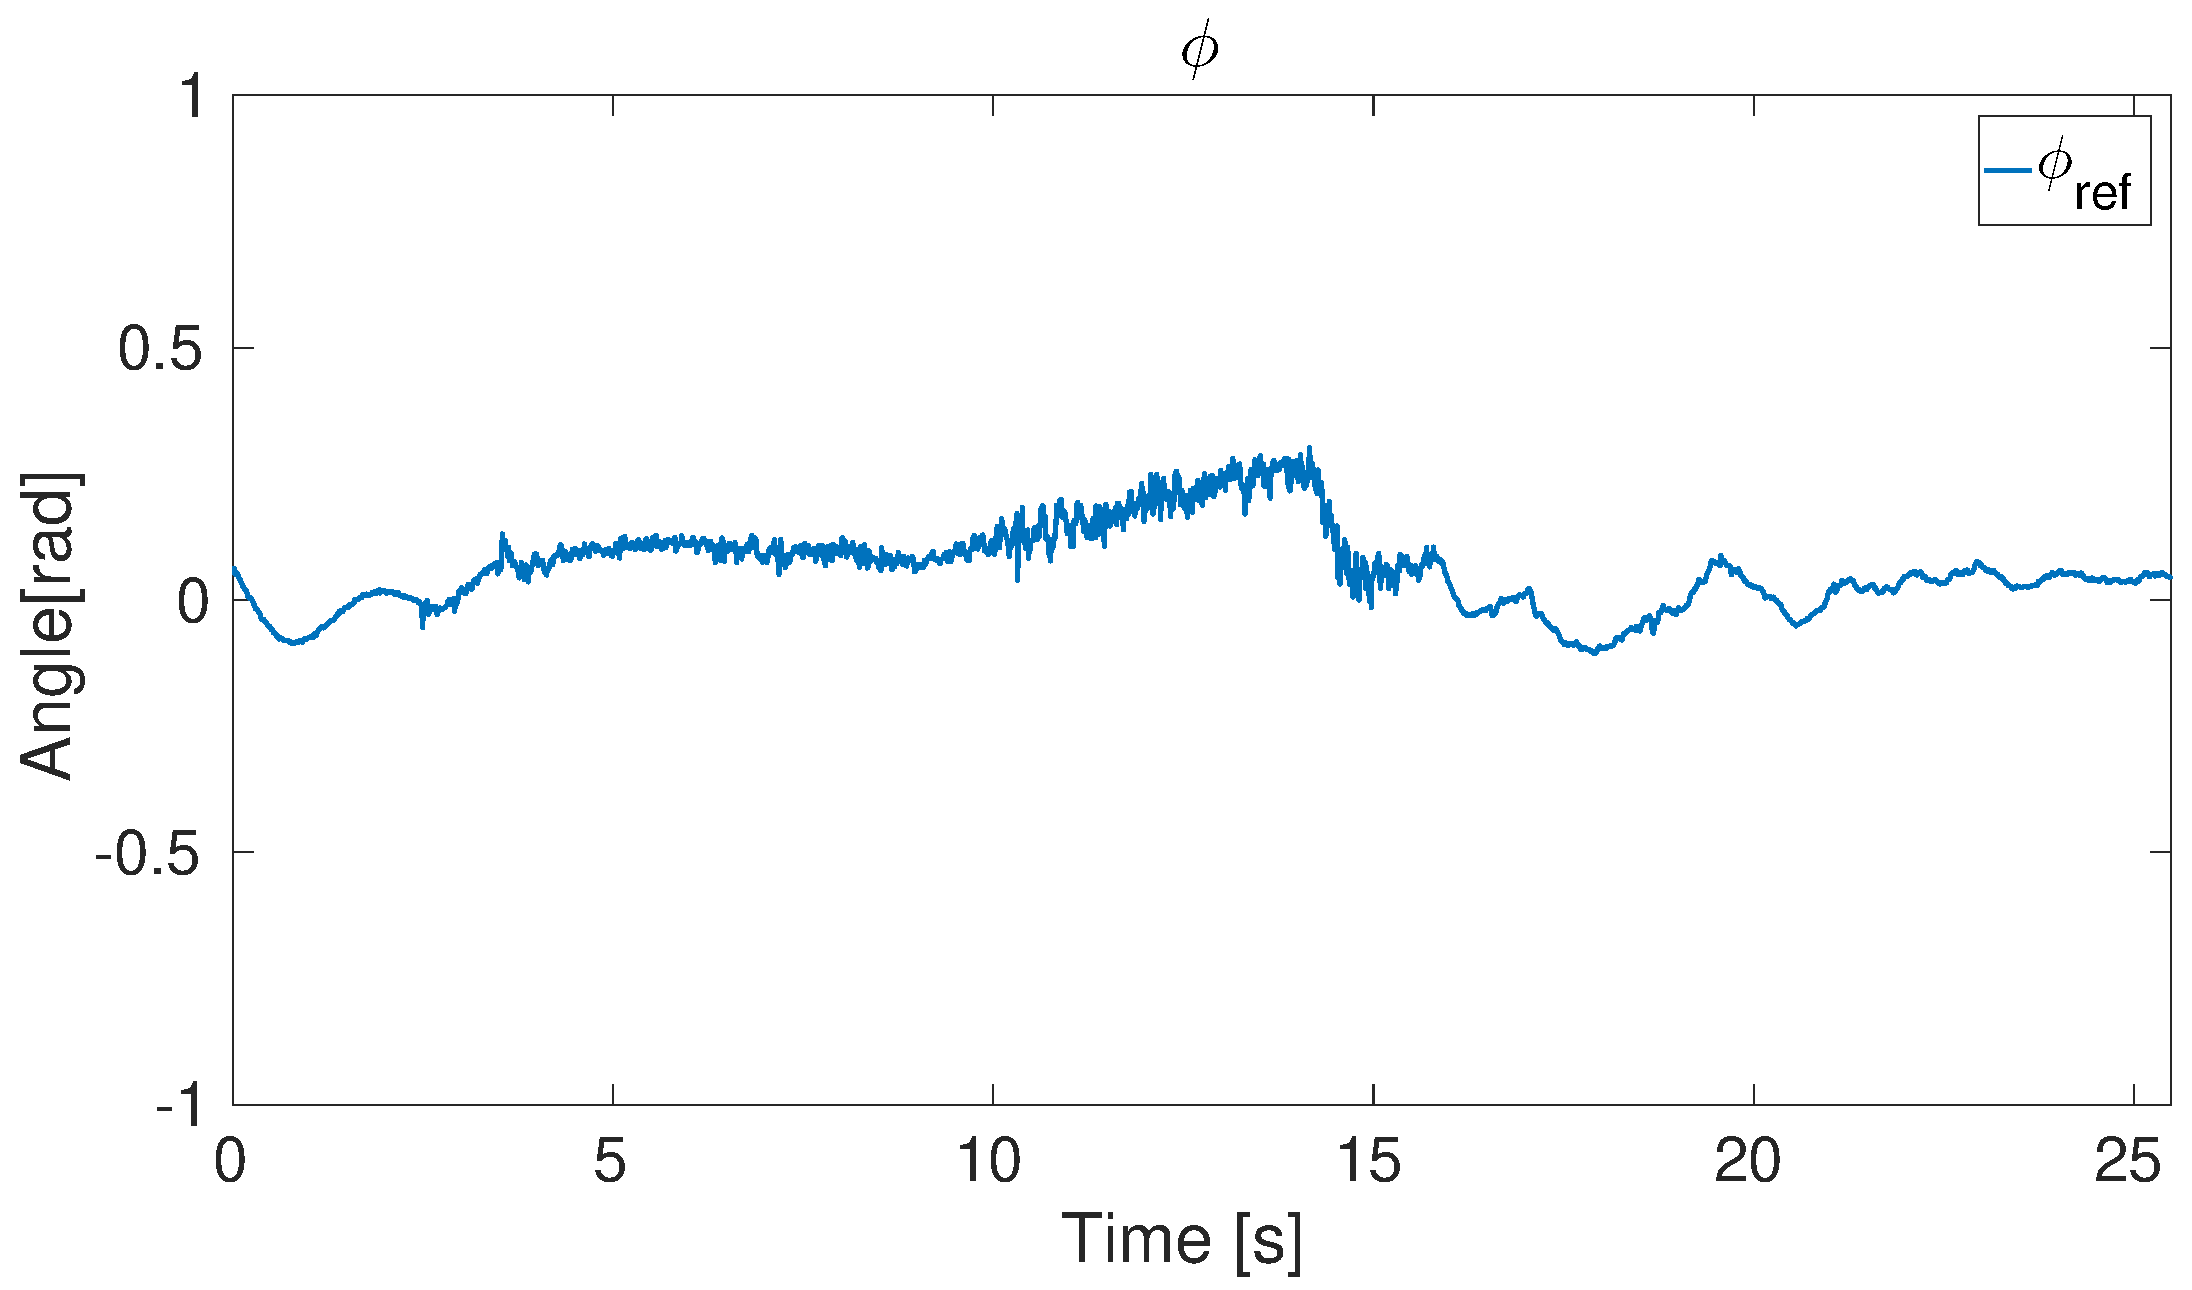
\includegraphics[width=0.4\textwidth]{testExactLinAttitudePhi}}
  \qquad
  \subfloat[][\label{fig:testExactAttitudePitch} The exact linearisation in $\pitchAngle$.]{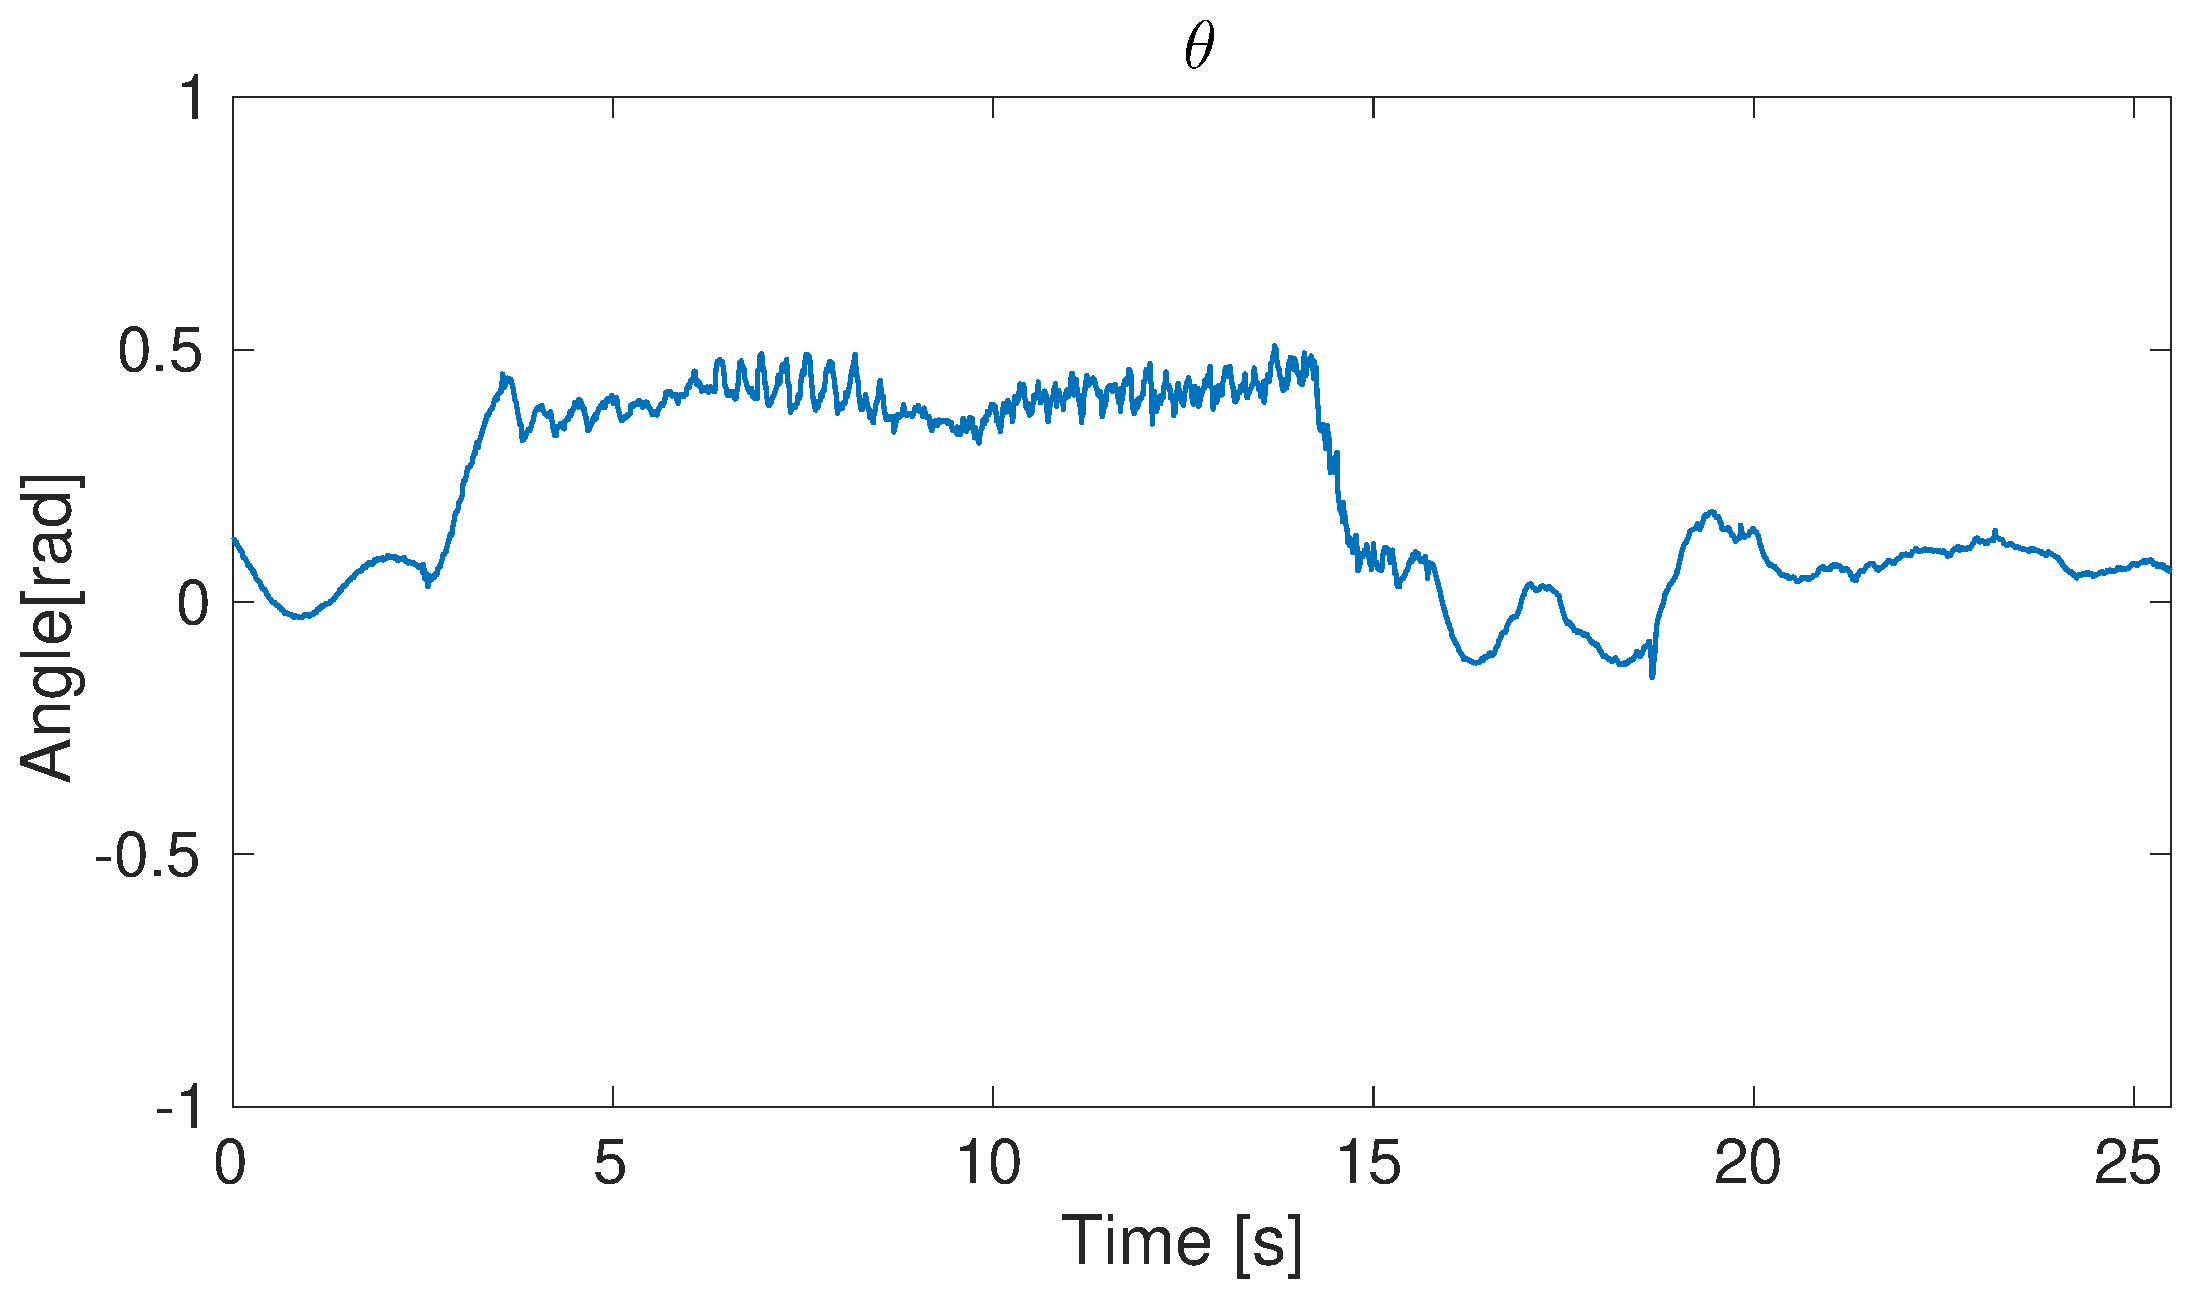
\includegraphics[width=0.4\textwidth]{testExactLinAttitudeTheta}}
  \qquad
  \subfloat[][\label{fig:testExactAttitudeYaw} The exact linearisation in $\yawAngle$.]{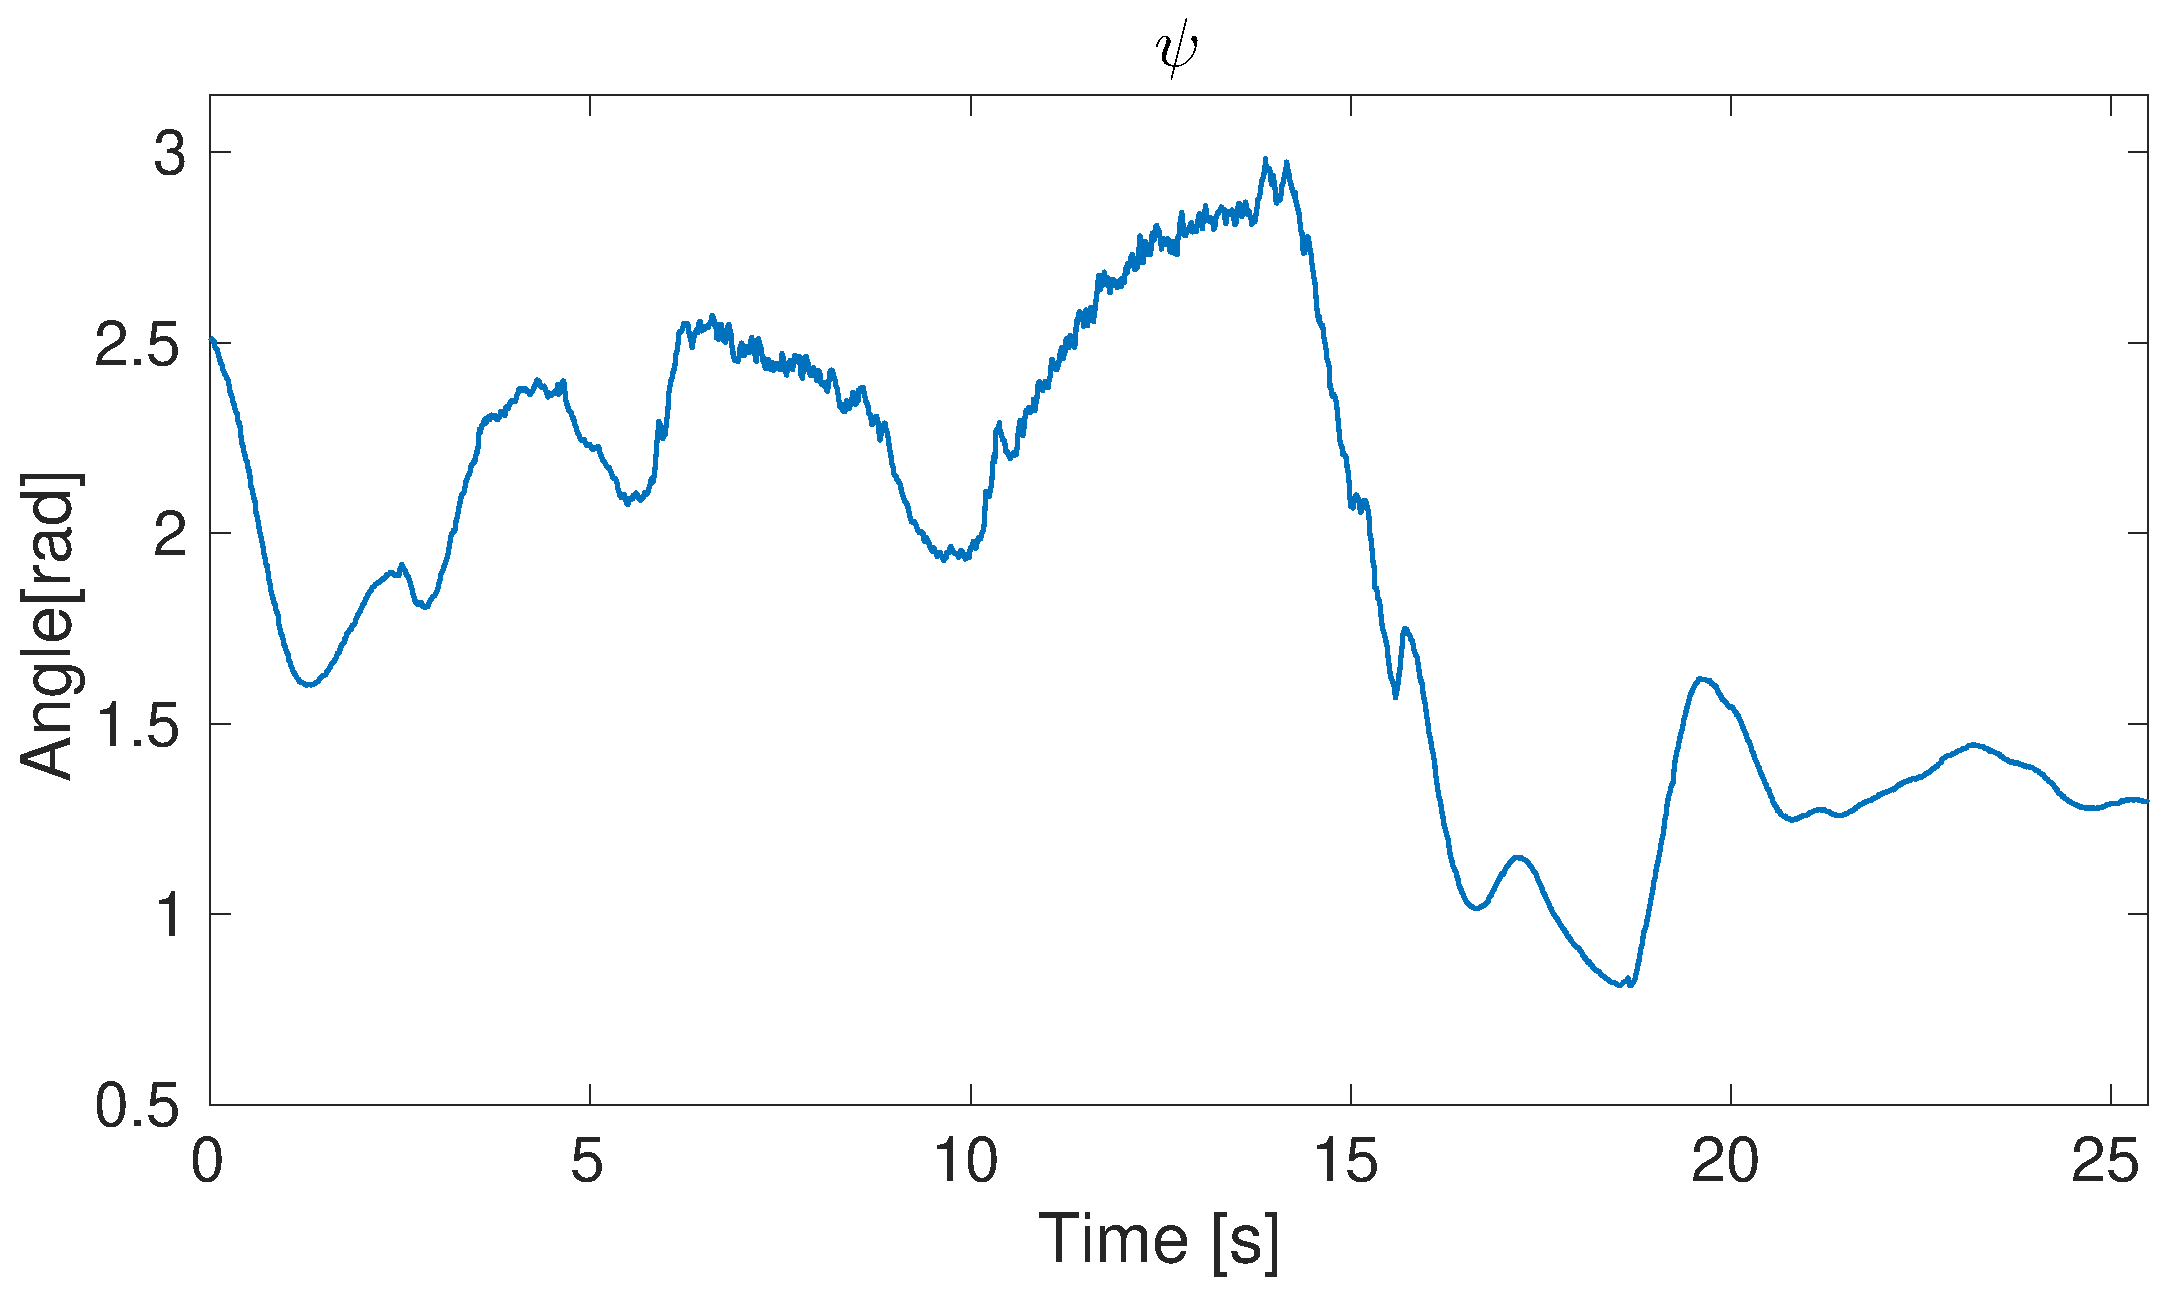
\includegraphics[width=0.4\textwidth]{testExactLinAttitudePsi}}
  \caption{\label{fig:ExactLinAttitude}% 
  The result of the exact linearisation attitude controller with setpoint $\phi_{ref}=0$, $\theta_{ref}=0$ and $\psi_{ref}=0$. Note the instability in $\theta$ and $\psi$.}
\end{figure}
Problems were encountered during trimming of the attitude \abbrPID using exact linearisation,
\Figureref{fig:ExactLinAttitude} shows this problem. Regardless of the strength of the feedback the \abbROV never stabilized. This problem might be caused by the magnetometer readings, which fluctuated mildly when the \abbrROV  engaged its thrusters. It is suspected that such fluctuations in magnetic field strength may cause rapid changes in the estimated quaternions and angular velocities, leading to problems when computing \eqref{eq:anLaw} in the exact-linearisation block. 
%%%%%%%%%%%%%%%%%%%%%%%%%%%Attitude%%%%%%%%%%%%%%%%%

\begin{figure}
\centering
  \subfloat[][\label{fig:testStepAllRollAttitude} A smooth step applied in $\rollAngle$.]{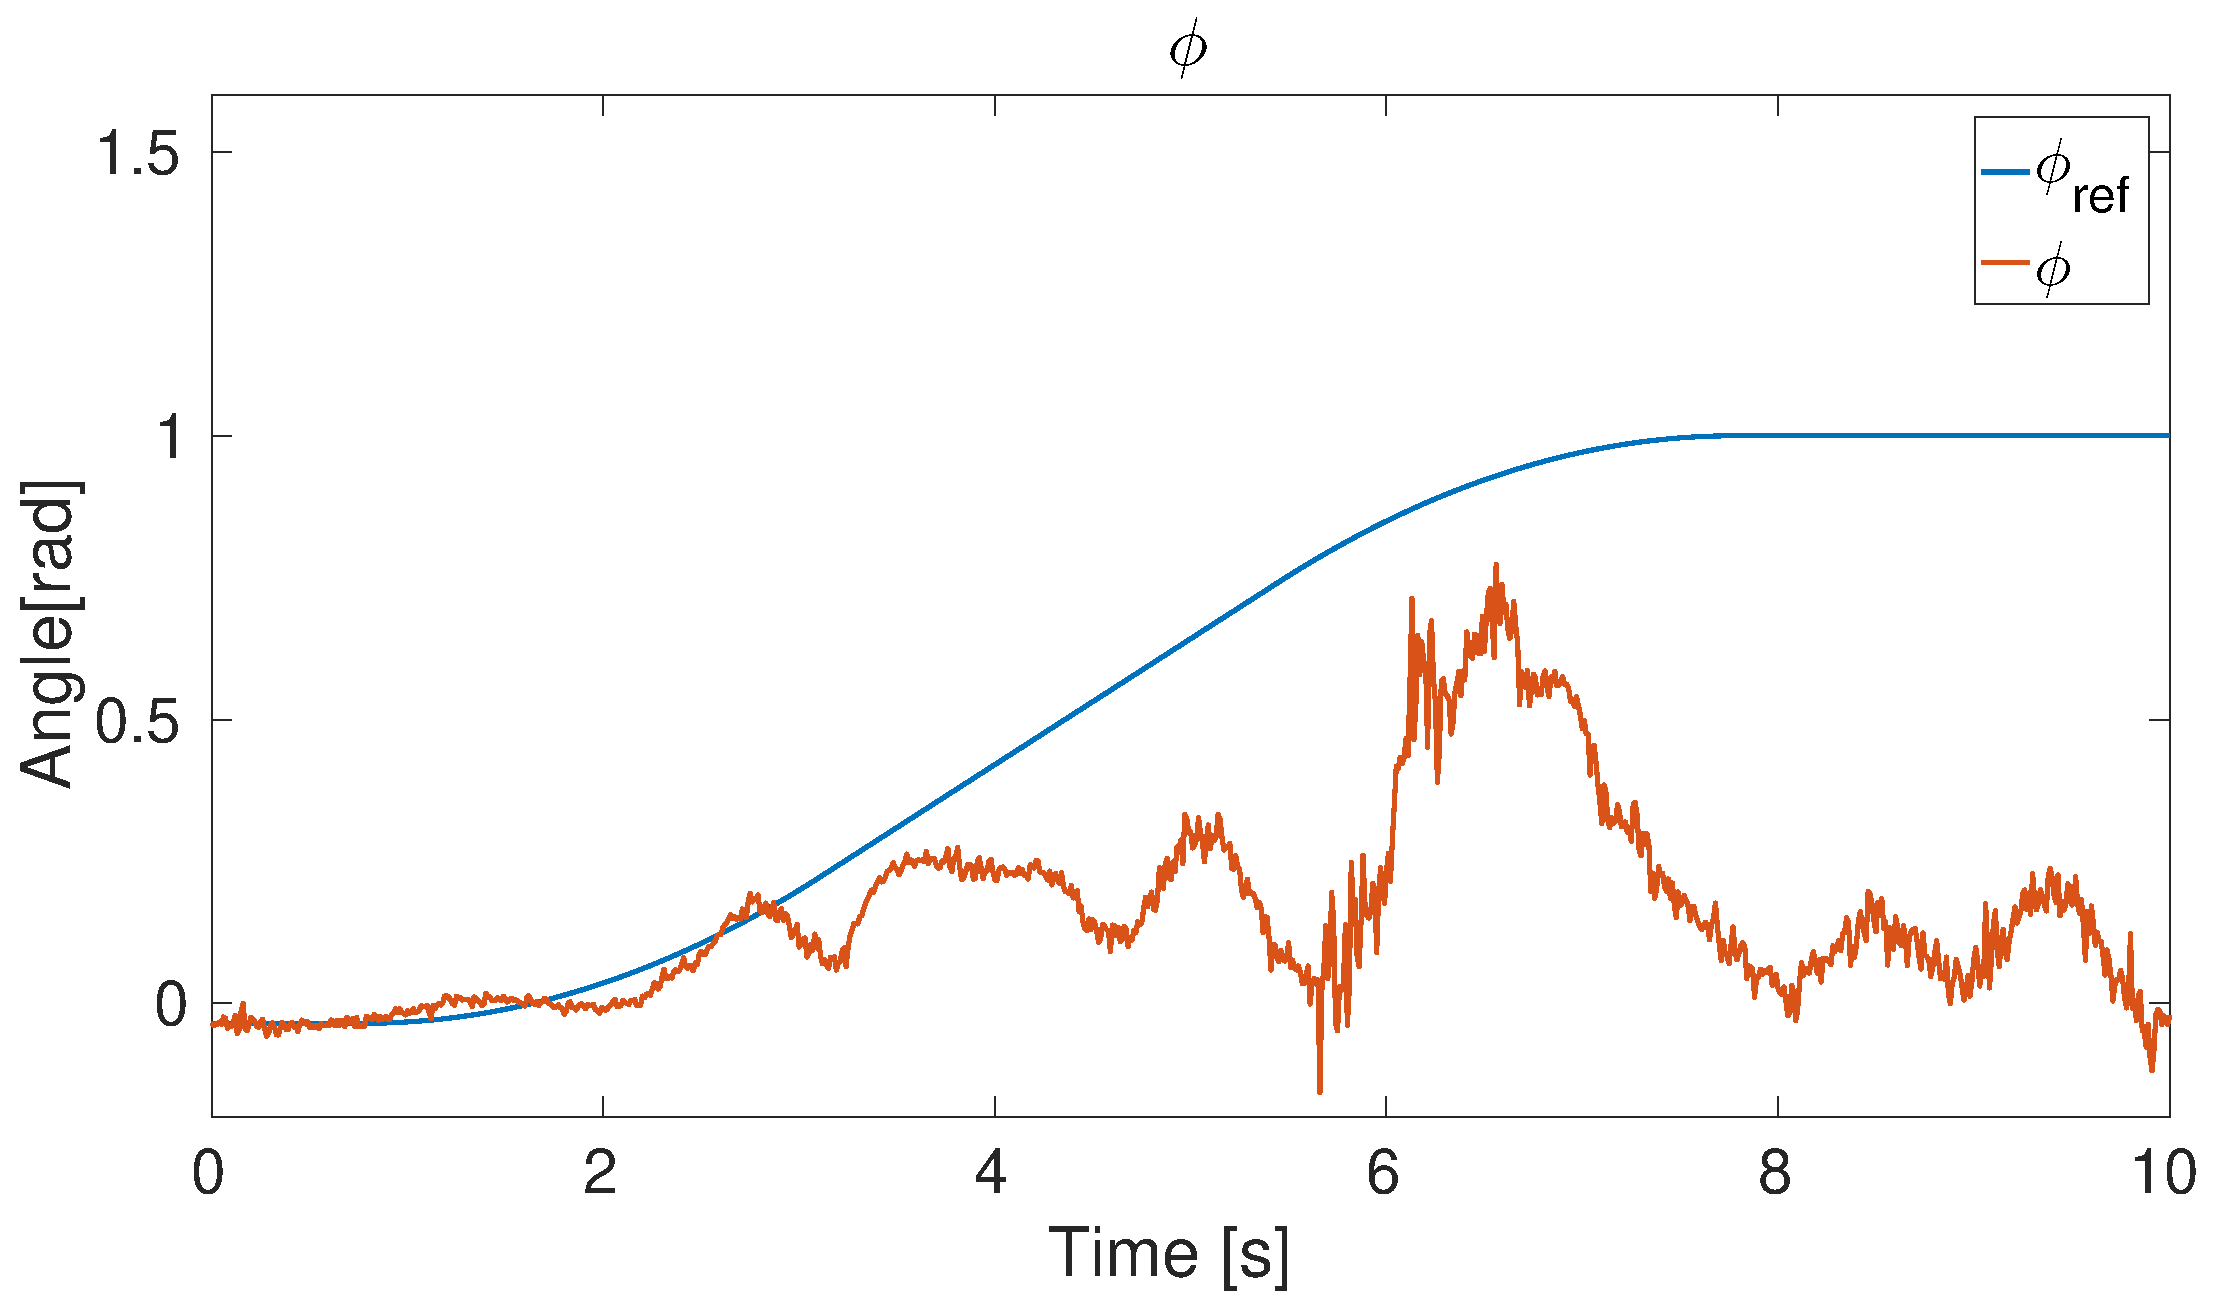
\includegraphics[width=0.4\textwidth]{testStepAllPhis3e10a1}}
  \qquad
  \subfloat[][\label{fig:simStepAllRollAttitude} A smooth step applied to the simulated \abbrROV in $\rollAngle$.]{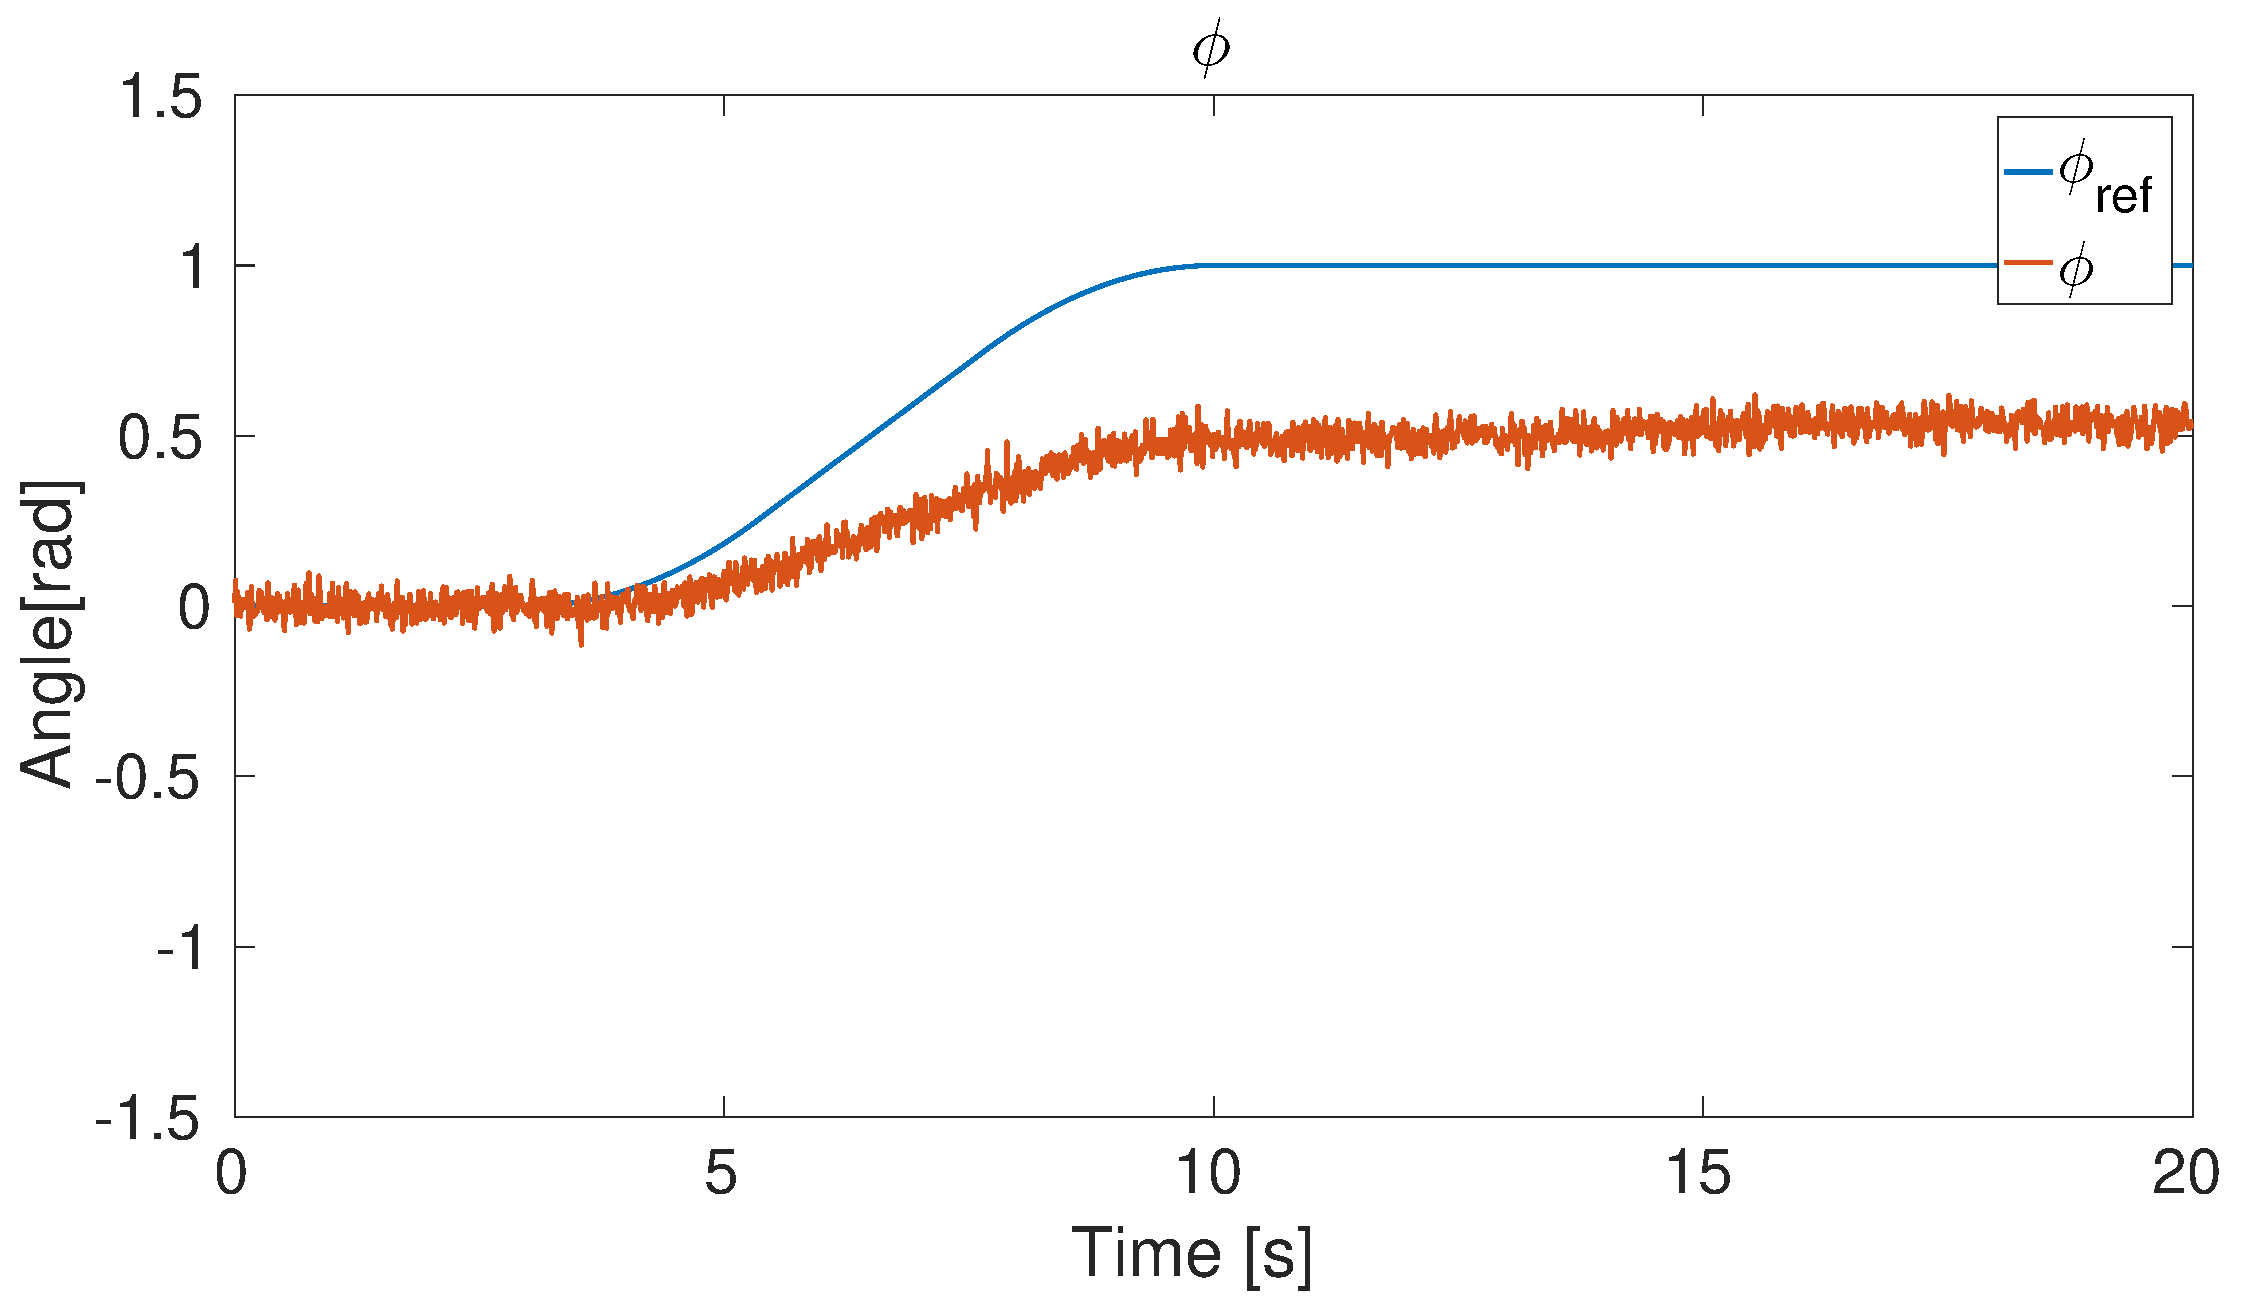
\includegraphics[width=0.4\textwidth]{simStepAllPhis3e10a1}}
  \qquad
  \subfloat[][\label{fig:TestStepAllPitchAttitude} A smooth step applied in $\pitchAngle$.]{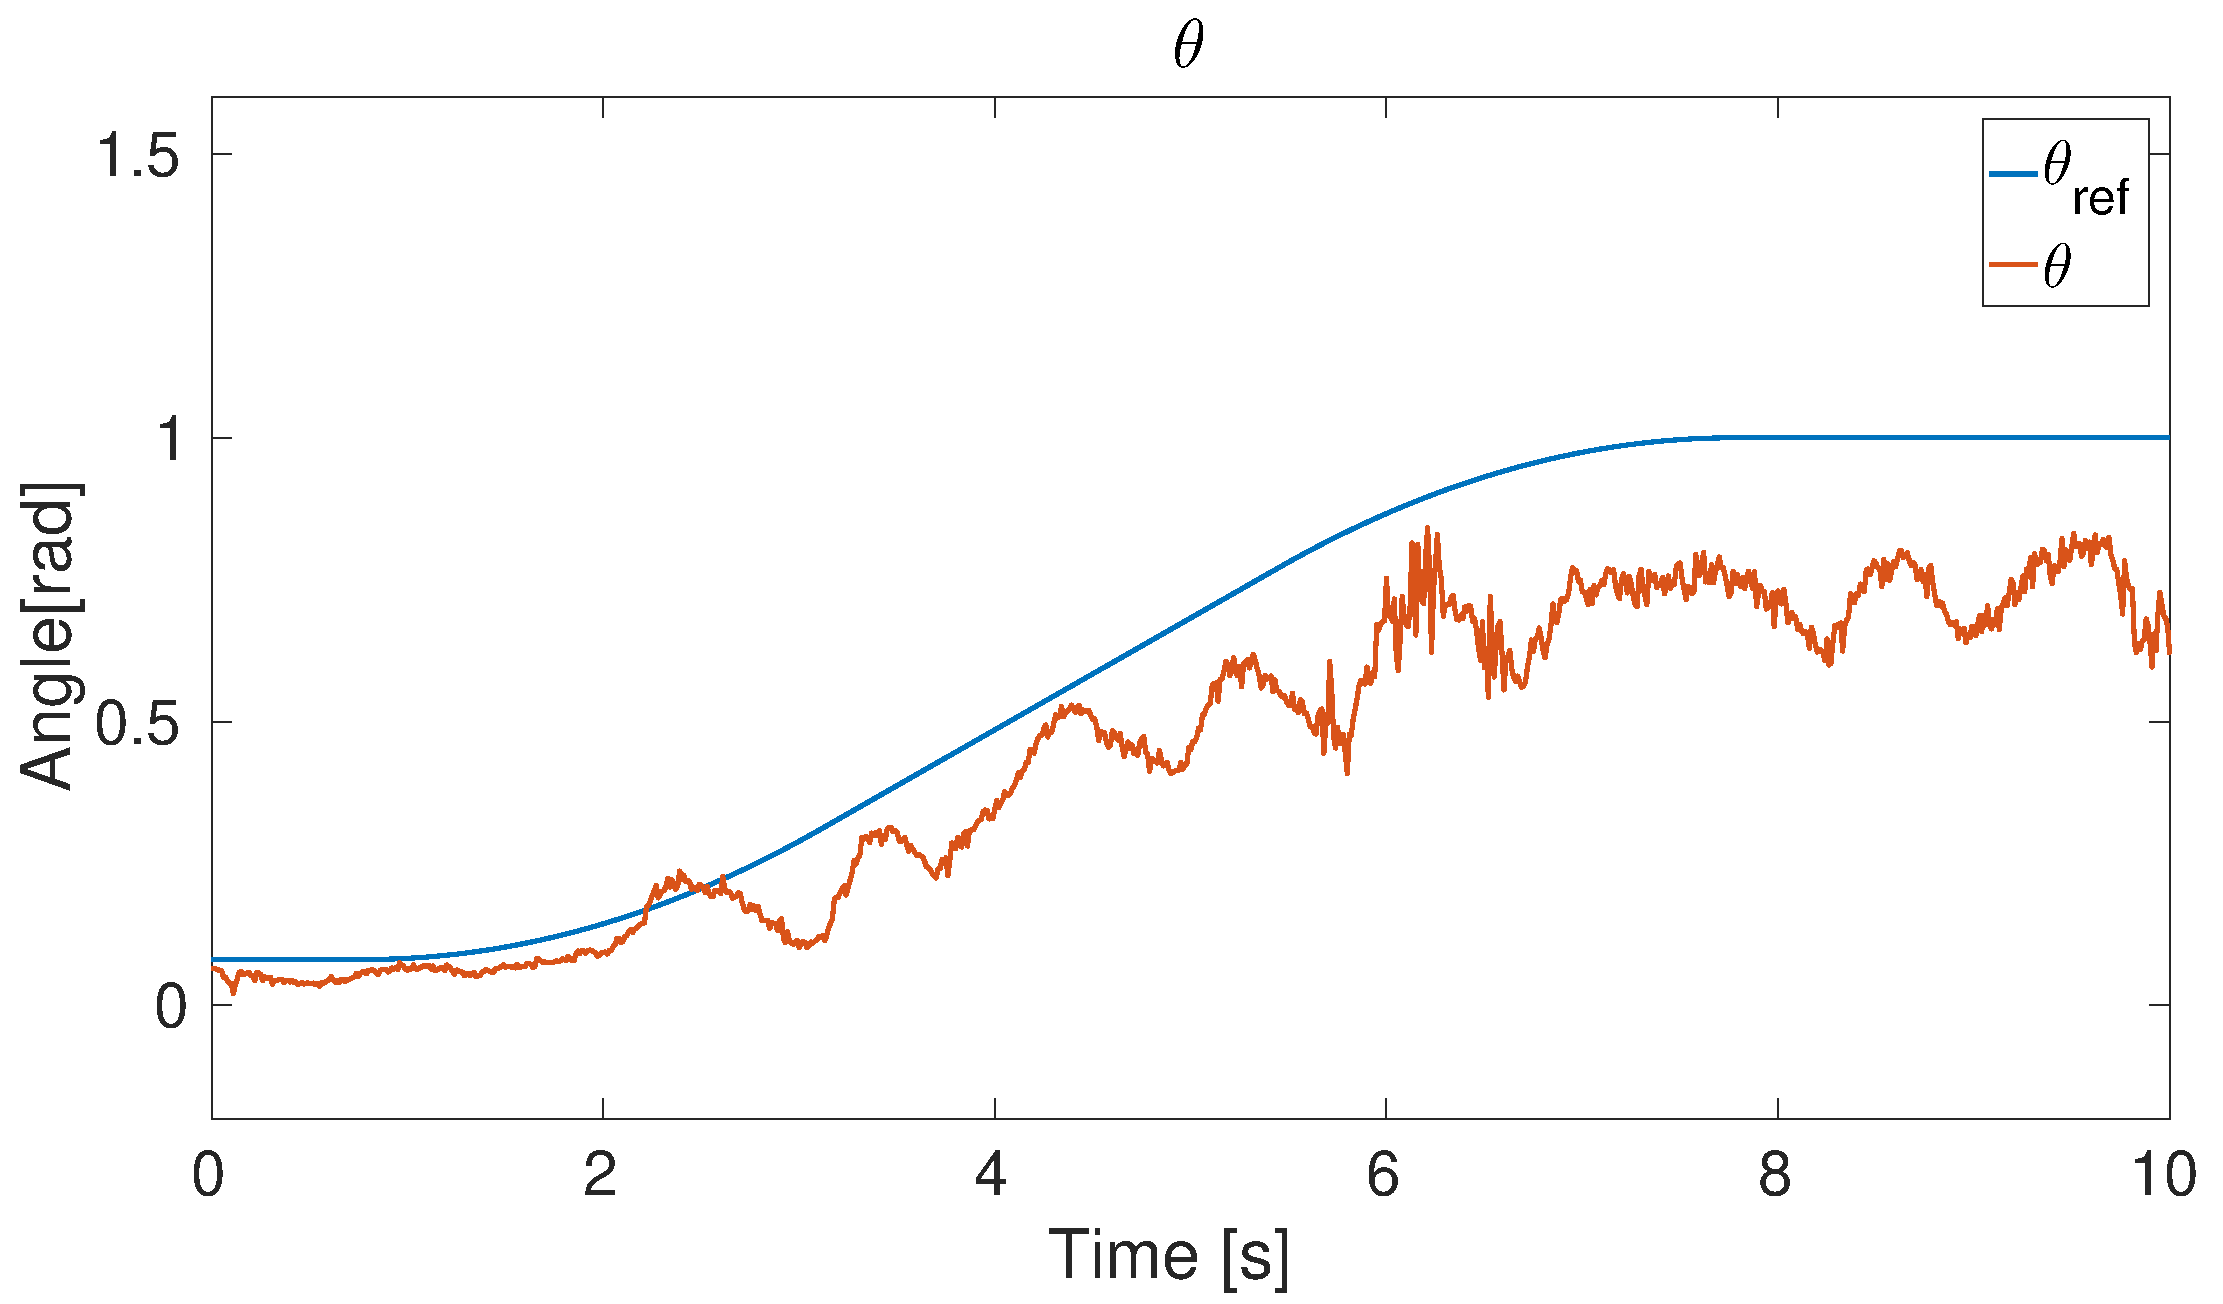
\includegraphics[width=0.4\textwidth]{testStepAllThetas3e10a1}}
  \qquad
  \subfloat[][\label{fig:simStepAllPitchAttitude} A smooth step applied to the simulated \abbrROV in $\pitchAngle$.]{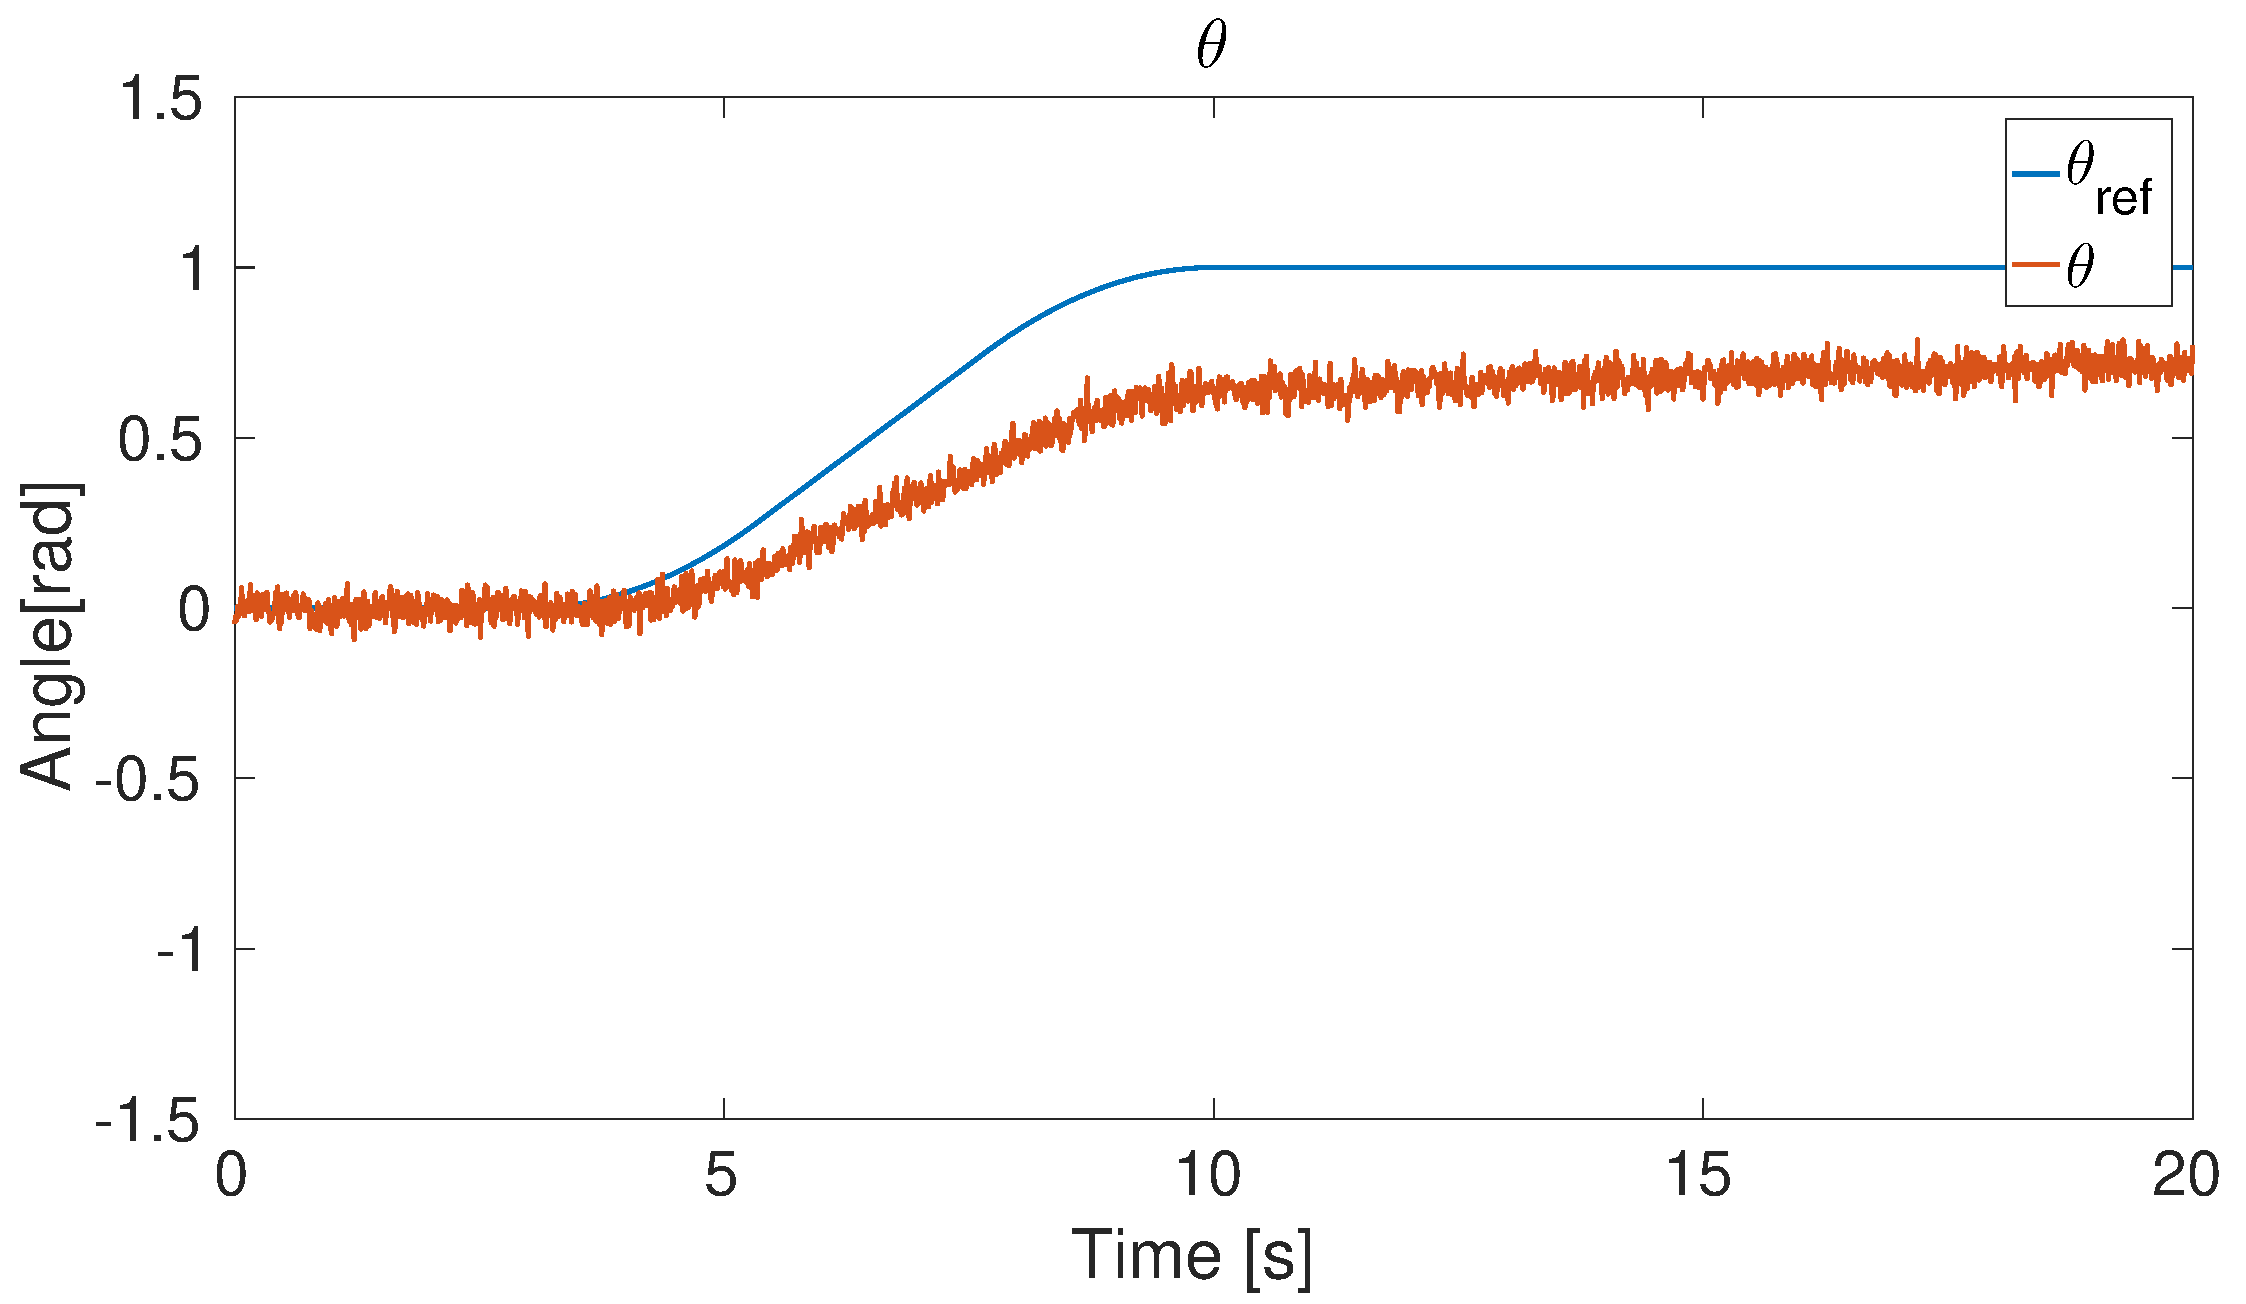
\includegraphics[width=0.4\textwidth]{simStepAllThetas3e10a1}}
  \qquad
  \subfloat[][\label{fig:TestStepAllYawAttitude} A smooth step applied in $\yawAngle$.]{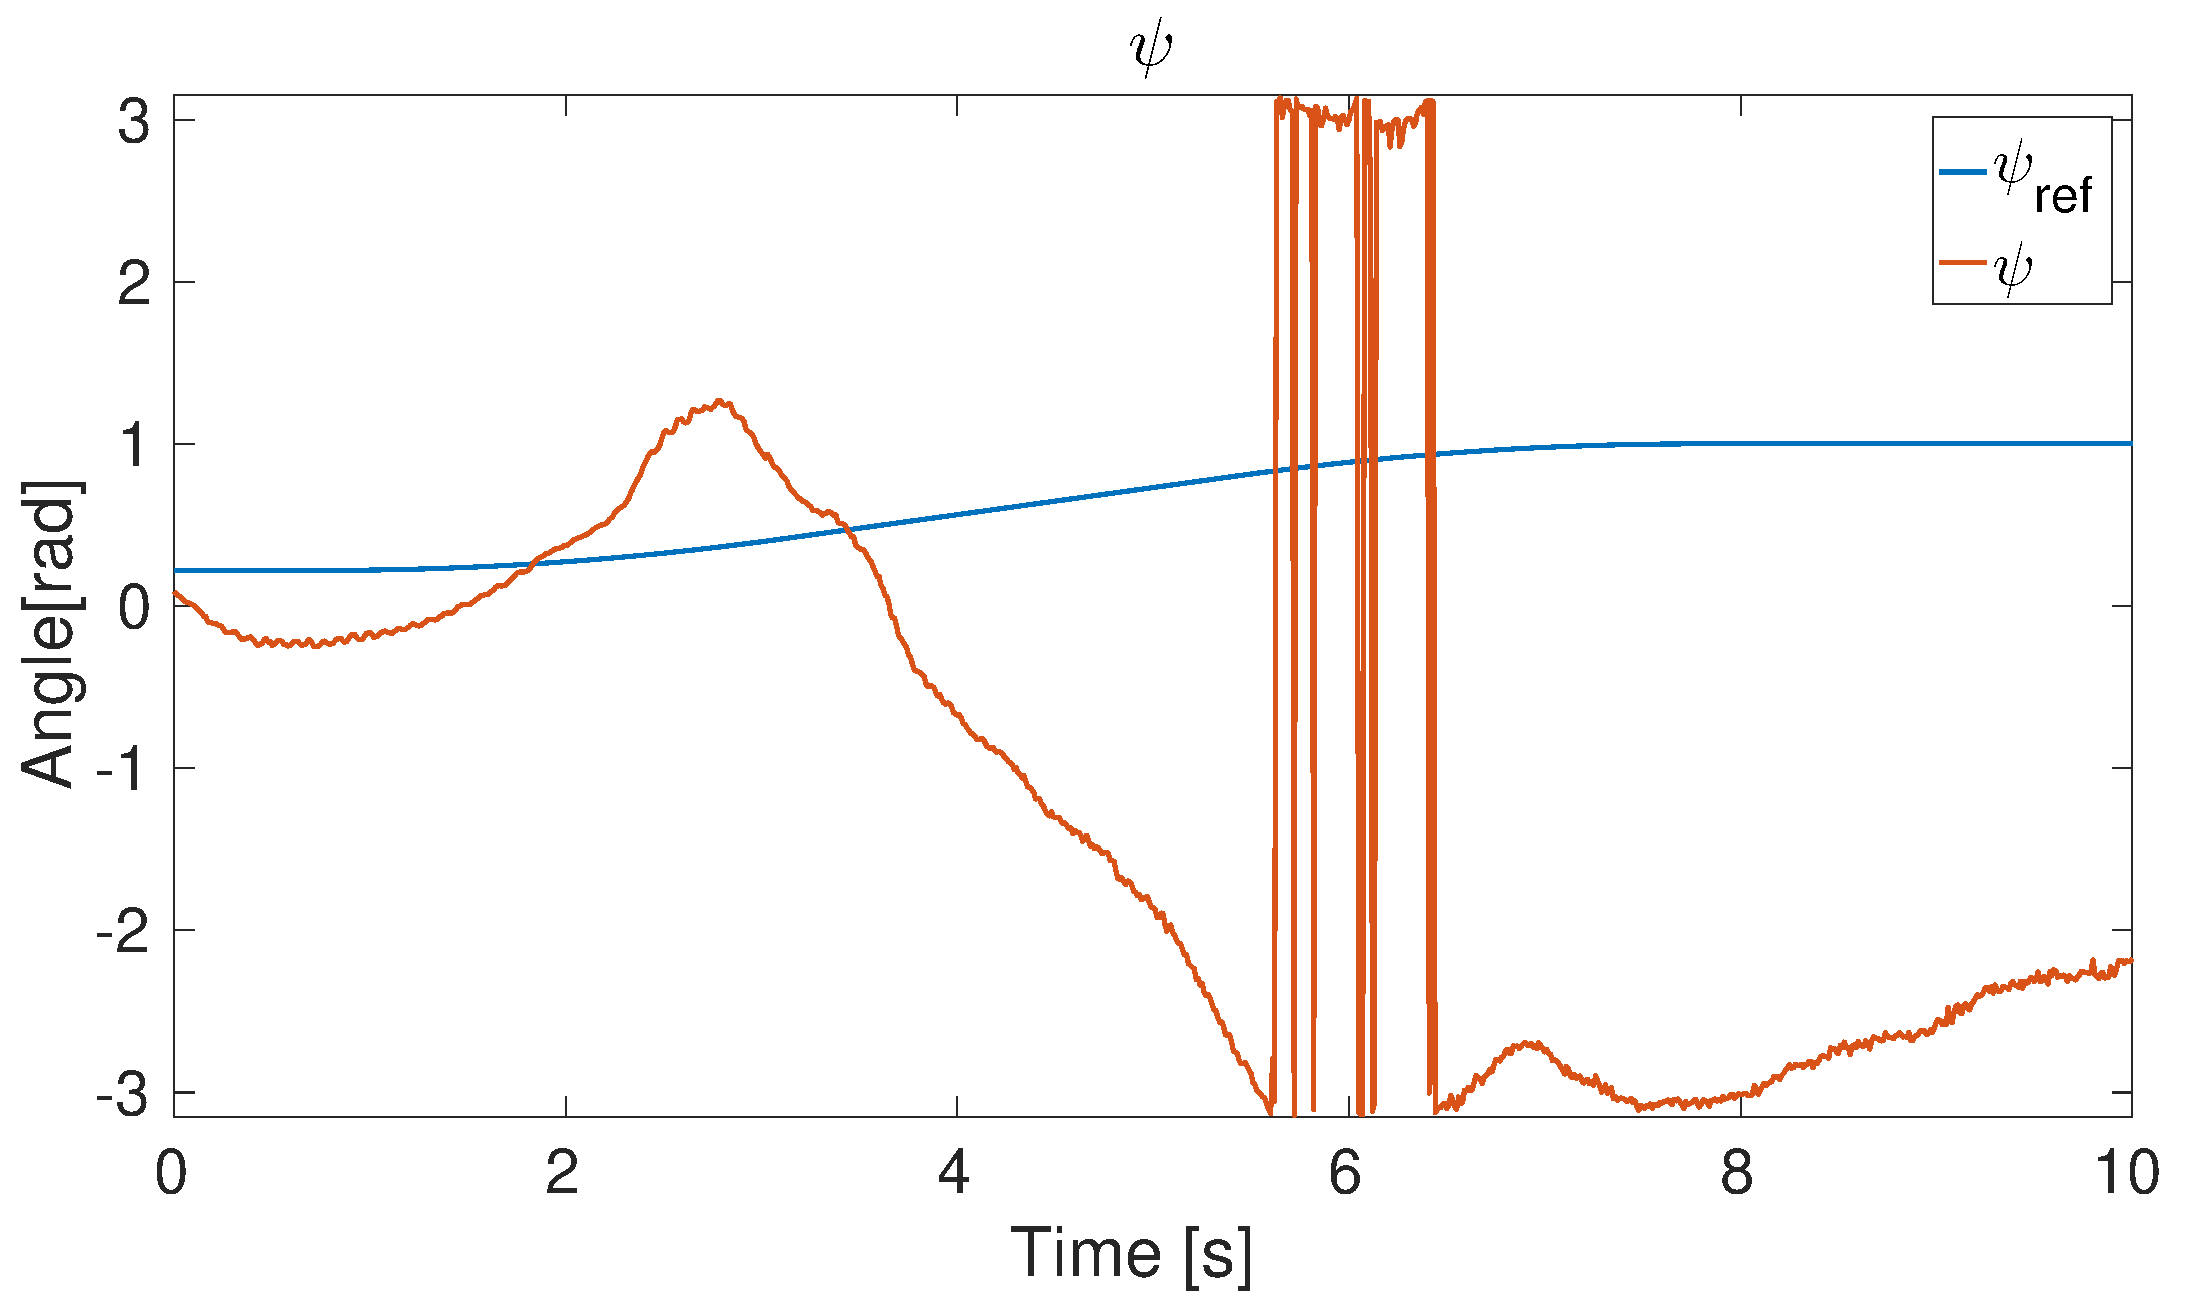
\includegraphics[width=0.4\textwidth]{testStepAllPsis3e10a1}}
  \qquad
  \subfloat[][\label{fig:simStepAllYawAttitude} A smooth step applied to the simulated \abbrROV in $\yawAngle$.]{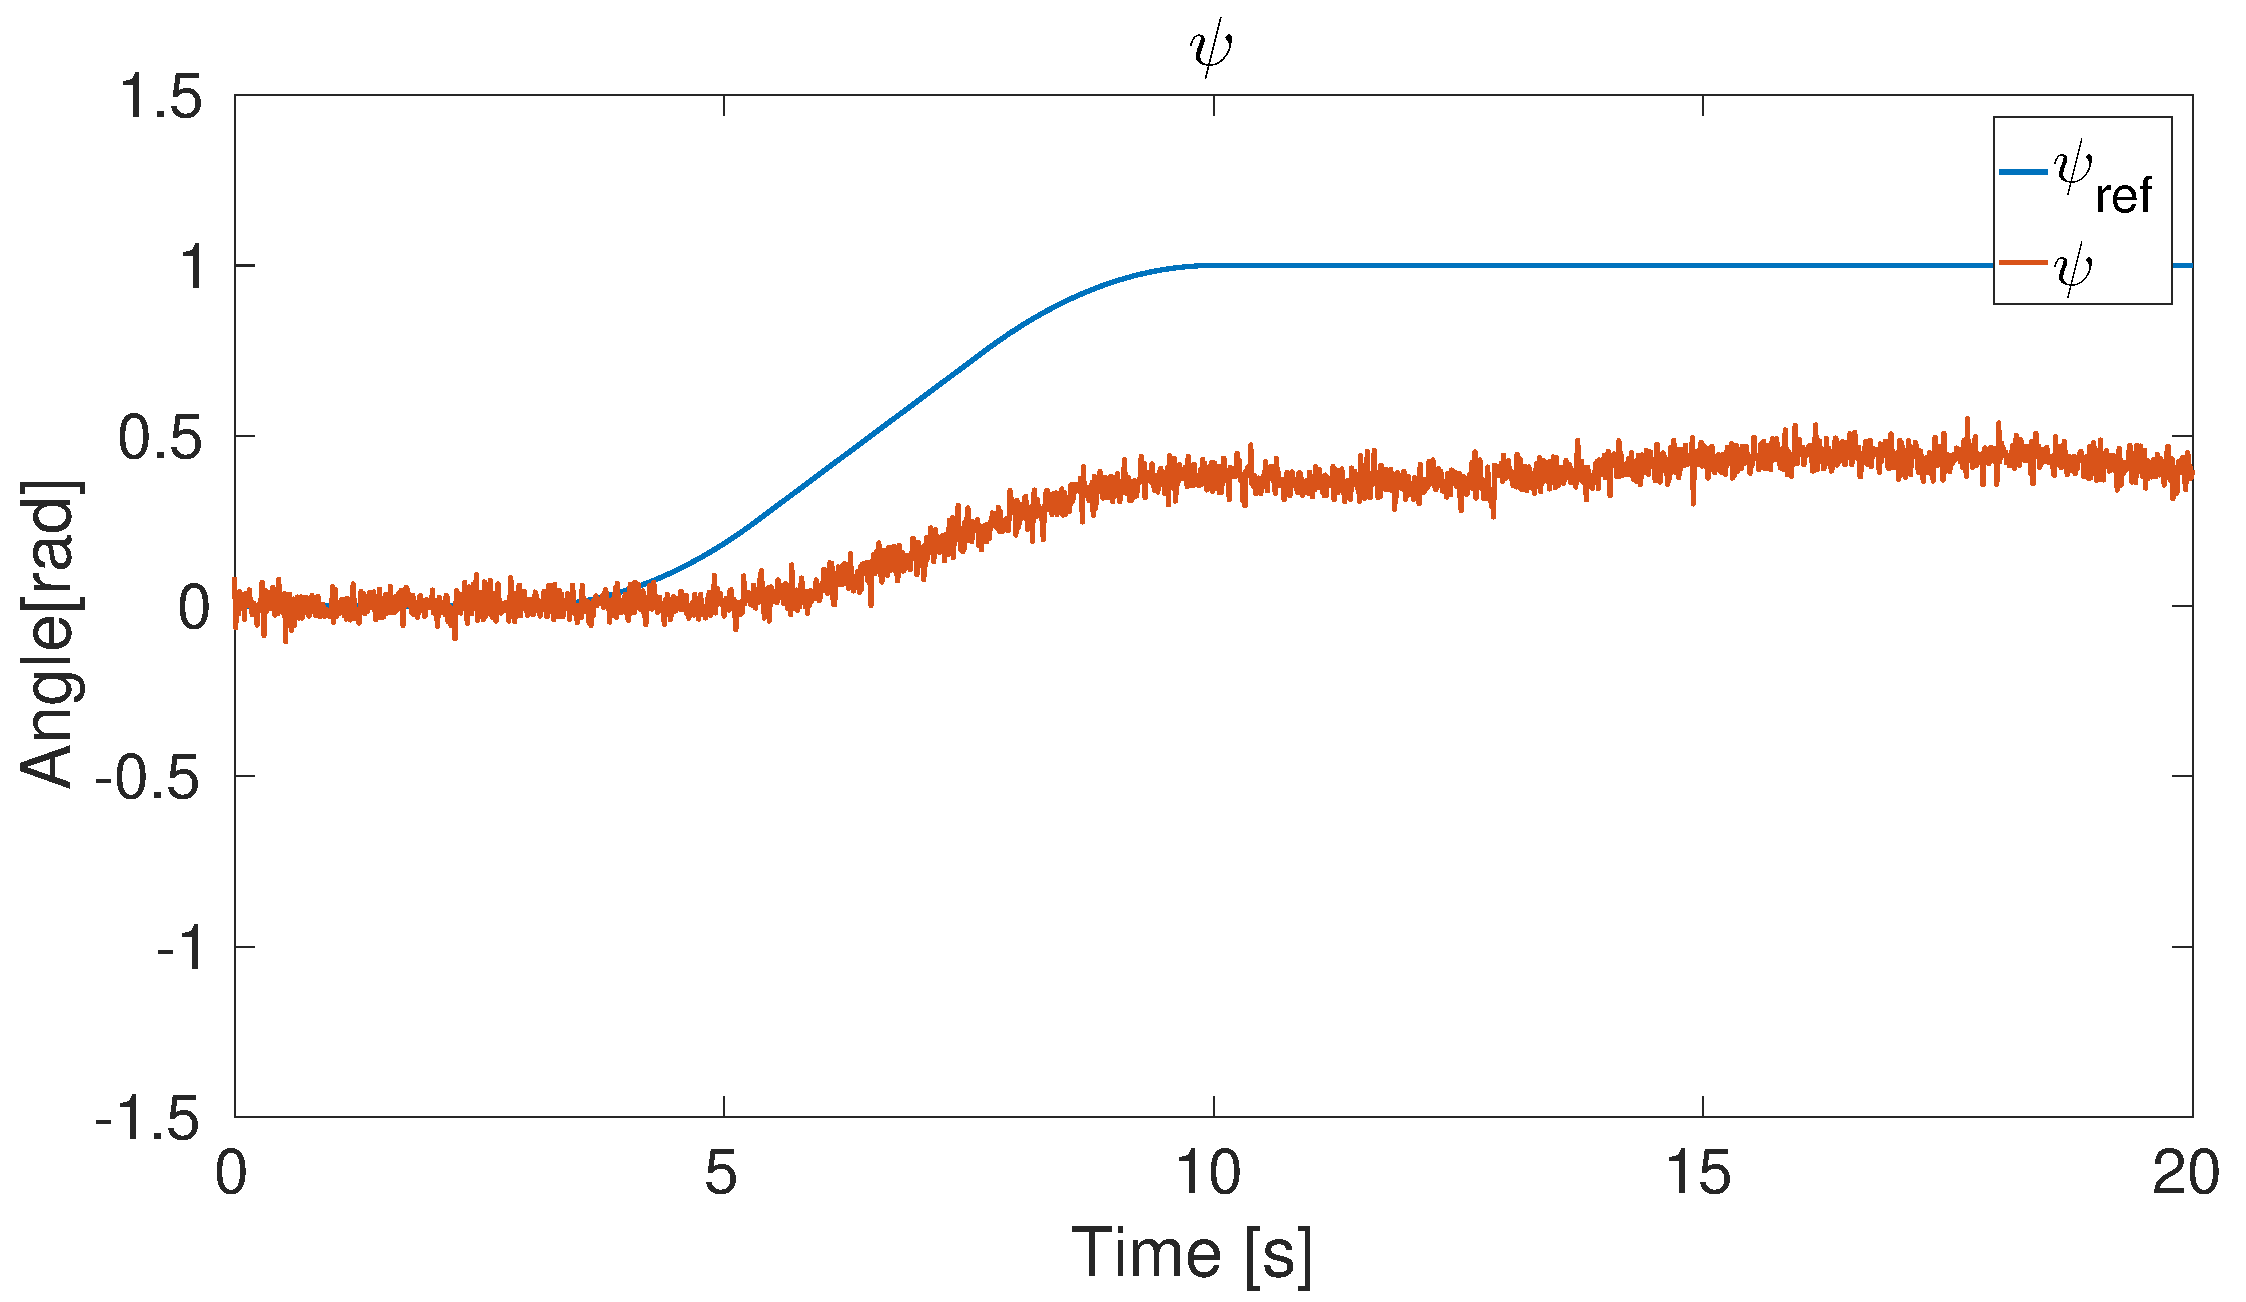
\includegraphics[width=0.4\textwidth]{simStepAllPsis3e10a1}}
  \caption{\label{fig:StepAllAttitude}% 
  Smooth steps were applied in all attitude angles at the same time while using the attitude controller.}
\end{figure}

\Figureref{fig:StepAllAttitude} shows smooth step reference signals applied in all attitude angles while using the attitude controller. Initially did $\rollAngle$ and $\pitchAngle$ follow the reference signals well in the real test. The $\rollAngle$ oscillated with a steady state error of 0.9 in the real test. However, $\pitchAngle$ was kept closer to the reference signal with a steady state error of 0.4. The attitude angle $\yawAngle$ could not be stabilised during the real test and drifted throughout the test. In the simulated test case did not the attitude angles reach the reference signal. The attitude angle $\pitchAngle$ had a steady state error of 0.3 and the other angles had a steady state error of 0.5.

\begin{figure}
\centering
  \subfloat[][\label{fig:testSinAllRollAttitude} A sine signal with amplitude $1$ and frequency $0.5\hertz$ applied in $\rollAngle$.]{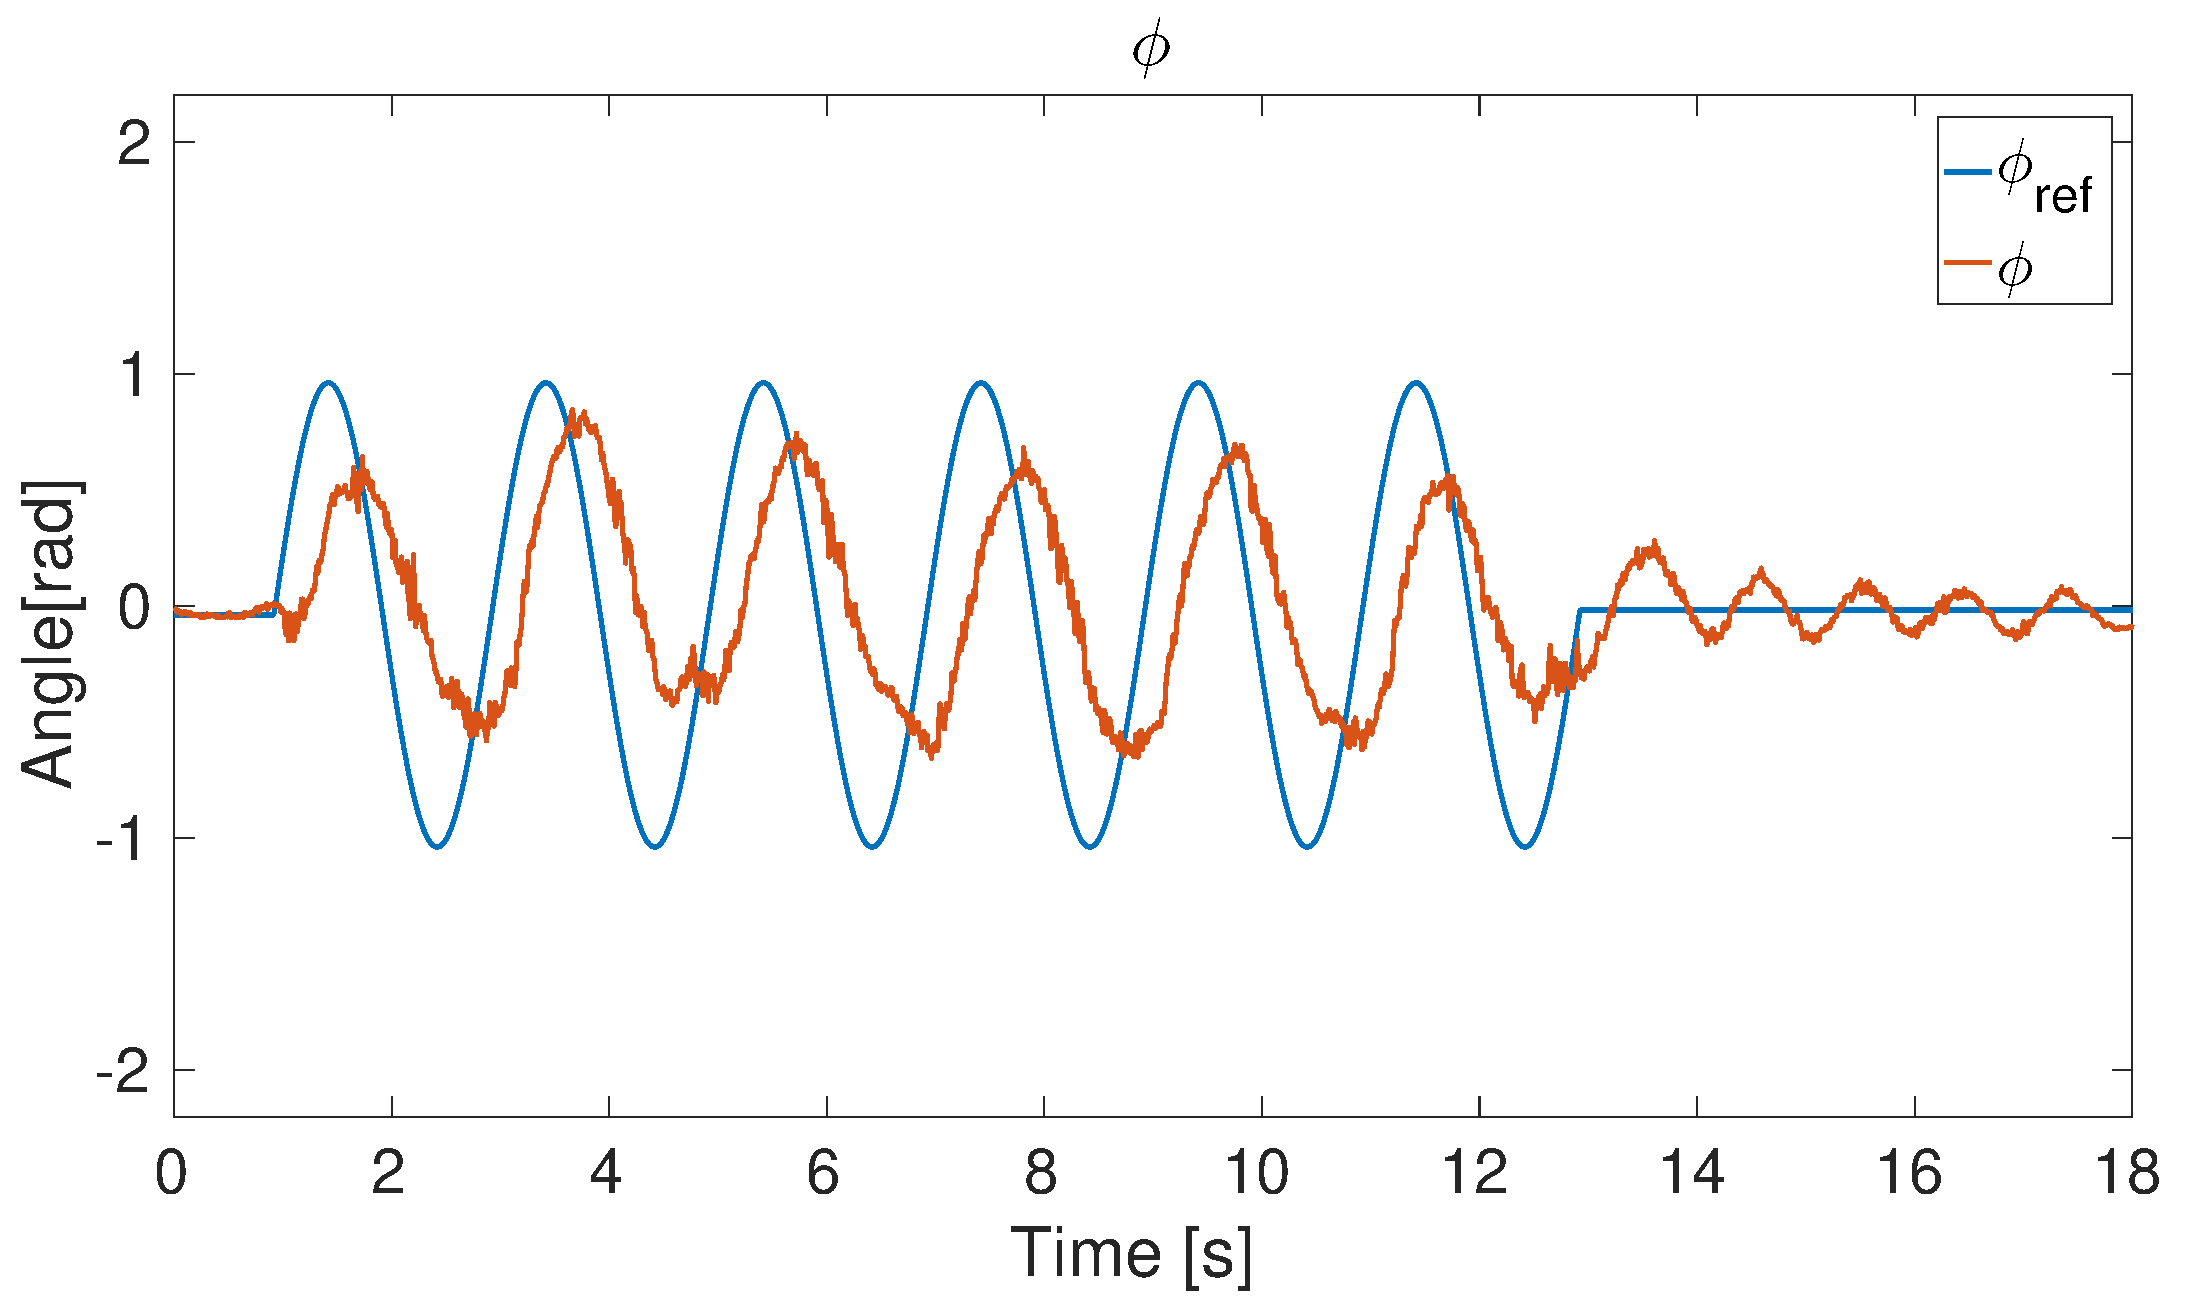
\includegraphics[width=0.4\textwidth]{testSinAllPhiA1}}
  \qquad
  \subfloat[][\label{fig:simSinAllRollAttitude} A sine signal with amplitude $1$ and frequency $0.5\hertz$ applied to the simulated \abbrROV in $\rollAngle$.]{\includegraphics[width=0.4\textwidth]{simSinAllPhiA1}}
  \qquad
  \subfloat[][\label{fig:testSinAllPitchAttitude} A sine signal with amplitude $1$ and frequency $0.5\hertz$ applied in $\pitchAngle$.]{\includegraphics[width=0.4\textwidth]{testSinAllThetaA1}}
  \qquad
  \subfloat[][\label{fig:simSinAllPitchAttitude} A sine signal with amplitude $1$ and frequency $0.5\hertz$ applied to the simulated \abbrROV in $\pitchAngle$.]{\includegraphics[width=0.4\textwidth]{simSinAllThetaA1}}
  \qquad
  \subfloat[][\label{fig:testSinAllYawAttitude} A sine signal with amplitude $1$ and frequency $0.5\hertz$ applied in $\yawAngle$.]{\includegraphics[width=0.4\textwidth]{testSinAllPsiA1}}
  \qquad
  \subfloat[][\label{fig:simSinAllYawAttitude} A sine signal with amplitude $1$ and frequency $0.5\hertz$ applied to the simulated \abbrROV in $\yawAngle$.]{\includegraphics[width=0.4\textwidth]{simSinAllPsiA1}}
  \caption{\label{fig:SinAllAttitude}%
  Sine signals were applied in all attitude angles at the same time while using the attitude controller.}
\end{figure}

Sine reference signals with amplitude 1 and frequency $0.5 \hertz$ can be seen in \Figureref{fig:SinAllAttitude}. The angles $\rollAngle$ and $\pitchAngle$ did not reached the assigned amplitude in the real test. However, did they have the general form of a sine but phase shifted relative to the reference signals. The $\yawAngle$ follows the reference signal well but with a phase shift and a bias. In simulation tests the same phase shift and lack of amplitude happened in $\rollAngle$ and $\pitchAngle$. The simulated result in $\yawAngle$ did not follow the reference signal at all. 

\begin{figure}
\centering
  \subfloat[][\label{fig:testStepPhiTheta05RollAttitude} A smooth step applied in $\rollAngle$.]{\includegraphics[width=0.4\textwidth]{testStepThetaPhiPhis3e10a1}}
  \qquad
  \subfloat[][\label{fig:simStepPhiTheta05RollAttitude} A smooth step applied to the simulated \abbrROV in $\rollAngle$.]{\includegraphics[width=0.4\textwidth]{simStepThetaPhiPhis3e10a1}}
  \qquad
  \subfloat[][\label{fig:testStepPhiTheta05PitchAttitude} A smooth step applied in $\pitchAngle$.]{\includegraphics[width=0.4\textwidth]{testStepThetaPhiThetas3e10a1}}
  \qquad
  \subfloat[][\label{fig:simStepPhiTheta05PitchAttitude} A smooth step applied to the simulated \abbrROV in $\pitchAngle$.]{\includegraphics[width=0.4\textwidth]{simStepThetaPhiThetas3e10a1}}
  \caption{\label{fig:StepPhiThetaAttitude}%
  Smooth steps were applied in \pitchAngle and \rollAngle at the same time while using the attitude controller. The attitude angle $\yawAngle$ was kept free during the test.}
\end{figure}

A smoothed step in $\rollAngle$ and $\pitchAngle$ can be seen in \Figureref{fig:StepPhiThetaAttitude}. During the test was the attitude angle $\yawAngle$ kept free. Both $\rollAngle$ and $\pitchAngle$ followed the reference signal well did not reach the reference angle. The steady state error for $\rollAngle$ and $\pitchAngle$ was approximately $0.35$. The simulated results in $\rollAngle$ and $\pitchAngle$ were worse than the real test. The attitude $\rollAngle$ had a steady state error 0.5 and the steady state error for $\pitchAngle$ was 0.4.

%%%%%%%%%%%%%%%%%%%%%%%%%%%Rate%%%%%%%%%%%%%%%%
\begin{figure}
\centering
  \subfloat[][\label{fig:testStepAllPRate} A smooth step applied in $\rollVelocity$.]{\includegraphics[width=0.4\textwidth]{testStepAllPs3e10a1}}
  \qquad
  \subfloat[][\label{fig:simStepAllPRate} A step applied to the simulated \abbrROV in $\rollVelocity$.]{\includegraphics[width=0.4\textwidth]{simStepAllPs3e10a1}}
  \qquad
  \subfloat[][\label{fig:testStepAllQRate} A smooth step applied in $\pitchVelocity$.]{\includegraphics[width=0.4\textwidth]{testStepAllQs3e10a1}}
  \qquad
  \subfloat[][\label{fig:simStepAllQRate} A step applied to the simulated \abbrROV in $\pitchVelocity$.]{\includegraphics[width=0.4\textwidth]{simStepAllQs3e10a1}}
  \qquad
  \subfloat[][\label{fig:testStepAllRRate} A smooth step applied in $\yawVelocity$.]{\includegraphics[width=0.4\textwidth]{testStepAllRs3e10a1}}
  \qquad
  \subfloat[][\label{fig:simStepAllRRate} A step applied to the simulated \abbrROV in $\yawVelocity$.]{\includegraphics[width=0.4\textwidth]{simStepAllRs3e10a1}}
  \caption{\label{fig:StepAllRate}% 
  Smooth steps were applied in all angular velocities at the same time while using the rate controller.}
\end{figure}

\Figureref{fig:StepAllRate} shows a smooth step applied in all angular velocities while using the rate controller. An overshoot of 0.5 is achieved in $\rollVelocity$ for the real test while in the simulation only has an overshoot of 0.2. Both the real test and the simulation in $\rollVelocity$ followed the reference signal well and had a small steady state error. The real and simulated test followed the reference value well in $\pitchVelocity$ and had negligible steady state errors. However, had the real test no overshoot while the simulation in $\pitchVelocity$ had an overshoot of 0.4. The simulated test in $\yawVelocity$ performed really well and almost followed the reference perfectly. The real test in $\yawVelocity$ performed well, but it was slow to rise to the requested reference signal and had a small steady state error of 0.1. 

\begin{figure}
\centering
  \subfloat[][\label{fig:testSinAllPRate} A sine signal with amplitude $1$ and frequency $0.5\hertz$ applied in $\rollVelocity$.]{\includegraphics[width=0.4\textwidth]{testSinAllPA1}}
  \qquad
  \subfloat[][\label{fig:simSinAllPRate}A sine signal with amplitude $1$ and frequency $0.5\hertz$ applied to the simulated \abbrROV in $\rollVelocity$.]{\includegraphics[width=0.4\textwidth]{simSinAllPA1}}
  \qquad
  \subfloat[][\label{fig:testSinAllQRate} A sine signal with amplitude $1$ and frequency $0.5\hertz$ applied in $\pitchVelocity$.]{\includegraphics[width=0.4\textwidth]{testSinAllQA1}}
  \qquad
  \subfloat[][\label{fig:simSinAllQRate} A sine signal with amplitude $1$ and frequency $0.5\hertz$ applied to the simulated \abbrROV in $\pitchVelocity$.]{\includegraphics[width=0.4\textwidth]{simSinAllQA1}}
  \qquad
  \subfloat[][\label{fig:testSinAllRRate} A sine signal with amplitude $1$ and frequency $0.5\hertz$ applied in $\yawVelocity$.]{\includegraphics[width=0.4\textwidth]{testSinAllRA1}}
  \qquad
  \subfloat[][\label{fig:simSinAllRRate} A sine signal with amplitude $1$ and frequency $0.5\hertz$ applied to the simulated \abbrROV in $\yawVelocity$.]{\includegraphics[width=0.4\textwidth]{simSinAllRA1}}
  \caption{\label{fig:SinAllRate}%
  Sine signals were applied in all angular velocities at the same time while using the rate controller.}
\end{figure}

Sine signals were applied to all angular velocities which can be seen in \Figureref{fig:SinAllRate} while using the rate controller. In the real test followed all the angular velocities the reference signals well, except for some overshoots and undershoots of the requested amplitude. The simulated test followed a general sine form but the reference amplitude was not reach and a phase shift could be noted.

%%%%%%%%%%%%%%%%%%%%%%%%%%%Depth%%%%%%%%%%%%%%%%
\begin{figure}[tbp]
  \centering
  \subfloat[][\label{fig:testStepD1} A smooth step applied in $\zPosition$.]{\includegraphics[width=0.4\textwidth]{testStepDepth3e10a1}}
  \qquad
  \subfloat[][\label{fig:testStepD2} A step applied in $\zPosition$.]{\includegraphics[width=0.4\textwidth]{testConstantD1}}
  \caption{\label{fig:StepD}%
    Steps applied to $\zPosition$. A smooth step from $0.4 \meter$ to $1 \meter$ is shown in (a) and a step from $0.5 \meter$ to $2 \meter$ is shown in (b).}
\end{figure}

\Figureref{fig:StepD} shows a smooth step from $0.4 \meter$ to $1 \meter$ and a step from $0.5 \meter$ to $2 \meter$. A delay in the response can be seen and overshoots of approximately 0.2.

%%%%%%%%%%%%%%%%%%%%%%%%%%%%%%%%%%%%%%%%
\section{Discussion}


\chapter{Conclusions and Future Work}\label{cha:conclusions}
In this thesis, has an attitude model for a \abbrROV been estimated. The model has then been used in controller synthesis to get satisfactory performance from the controllers. This chapter discuss and summarise the results from \Chapterref{cha:modelling} - \Chapterref{cha:controller}. 
Lastly, is there a presentation of ideas for future work and development.

%%%%%%%%%%%%%%%%%%%%%%%%%%%%%%%%%%%%%
\section{Conclusions}

%%%%%%%%%%%%%%%%%%%%%%%%%%%%%%%%%%%%%
\section{Future Work}
To get a better model of the \abbrROV an estimate of the \abbrROV's linear velocities. This 


\part*{Appendix}
\appendix
\chapter{Dependencies and Installation}\label{app:dependencies}
The following dependencies are some of the needed packages for compiling and running the \abbrROV.
\begin{itemize}
    \item Ubuntu 14.04
    \item ROS Indigo Igloo
    \item rosserial (Indigo)
    \item rosserial\_arduino (Indigo)
    \item image\_common (Indigo) 
    \item image\_transport (Indigo)
    \item joy (Indigo)
\end{itemize}

More details of the necessary packages are listed in the installation guide.

%%%%%%%%%%%%%%%%%%%%%%%%%%%%%%%%%%%%%%%%%%%%%%%%%%%%%%%%%%%%%%%%%%%%%%%%%%%%%%%%%%%
\section{Raspberry Pi installation}
This section summarises how to setup the Raspberry Pi. It is assumed that the Raspberry Pi is already running Ubuntu 14.04.

\subsection{\abbrROS Installation}
To install \abbrROS the \abbrROS source needs to be in the source listing run

\begin{lstlisting}[language=bash]
sudo sh -c 'echo "deb http://packages.ros.org/ros/ubuntu $(lsb_release -sc) main" > /etc/apt/sources.list.d/ros-latest.list' && sudo apt-get install ros-indigo-ros-base -y && sudo rosdep init && rosdep update && echo "source /opt/ros/indigo/setup.bash" >> ~/.bashrc && source ~/.bashrc && sudo apt-get upgrade -y && sudo ln -s /usr /opt/vc
\end{lstlisting}
to install \abbrROS and source the necessary files.

The packages needed and some other packages used in the \abbrROV is installed by
\begin{lstlisting}[language=bash]
sudo apt-get install libraspberrypi-bin libraspberrypi-dev openssh-server build-essential avahi-daemon linux-firmware python-rosinstall ros-indigo-rosserial ros-indigo-rosserial-arduino ros-indigo-image-common ros-indigo-image-transport-plugins git && sudo sh -c 'echo "start_x=1\ngpu_mem=128" >> /boot/config.txt'
\end{lstlisting}
then restart the Raspberry pi.

\subsection{Tether Setup}
For communication with the workstation the hostnames and Ethernet port needs to be setup.
Configure the host file 
\begin{lstlisting}
sudo nano /etc/hosts
\end{lstlisting}
add
\begin{lstlisting}
10.0.0.20 bluerov
10.0.0.10 workstation
\end{lstlisting}
to the host file. To use a static IP for the \abbrROV configure the interfaces file
\begin{lstlisting}
sudo nano /etc/network/interfaces
\end{lstlisting}
add 
\begin{lstlisting}
auto eth0
iface eth0 inet static
    address 10.0.0.20
    netmask 255.255.255.0
\end{lstlisting}
to the interfaces file. Reboot the computer or restart the networking services for changes to take effect.

\subsection{Installation of the \abbrROV package}
To download and to compile the package run
\begin{lstlisting}
git clone https://github.com/MrEkelund/ExjobbROV.git && cd ExjobbROV/catkin_ws && catkin_make && echo "source ~/path-to-package/ExjobbROV/catkin_ws/devel/setup.bash" >> ~/.bashrc 
\end{lstlisting}

Setup the communication with the arduino.
\begin{lstlisting}
sudo cp ExjobbROV/catkin_ws/src/bluerov/extra/99-bluerov.rules /etc/udev/rules.d/ && sudo udevadm trigger
\end{lstlisting}

Compile the arduino code and flash it to the arduino by running
\begin{lstlisting}
cd ExjobbROV/catkin_ws && catkin_make bluerov_arduino_firmware && catkin_make bluerov_arduino_firmware-upload
\end{lstlisting}

%%%%%%%%%%%%%%%%%%%%%%%%%%%%%%%%%%%%%%%%%%%%%%%%%%%%%%%%%%%%%%%%%%%%%%%%%%%%%%%%%%%
\section{Workstation Installation}
This section summarises how to setup the workstation for operation with the \abbrROV. It's assumed that the workstation is already running Ubuntu 14.04. 

\subsection{\abbrROS Installation}
To install \abbrROS run the following command
\begin{lstlisting}[language=bash]
sudo sh -c 'echo "deb http://packages.ros.org/ros/ubuntu $(lsb_release -sc) main" > /etc/apt/sources.list.d/ros-latest.list' && sudo apt-get install ros-indigo-ros-desktop-full && sudo rosdep init && rosdep update && echo "source /opt/ros/indigo/setup.bash" >> ~/.bashrc && source ~/.bashrc
\end{lstlisting}
then run 
\begin{lstlisting}
sudo apt-get install python-rosinstall ros-indigo-rosserial ros-indigo-rosserial-arduino ros-indigo-image-common ros-indigo-image-transport-plugins ros-indigo-joy sshpass git
\end{lstlisting}
to install some necessary packages.

\subsection{Tether Setup}
For communication with the \abbrROV the hostnames and Ethernet port needs to be setup.
Configure the host file 
\begin{lstlisting}
sudo nano /etc/hosts
\end{lstlisting}
add
\begin{lstlisting}
10.0.0.20 bluerov
10.0.0.10 workstation
\end{lstlisting}
to the host file. To use a static IP for the workstation configure the interfaces file
\begin{lstlisting}
sudo nano /etc/network/interfaces
\end{lstlisting}
add 
\begin{lstlisting}
auto eth0
iface eth0 inet static
    address 10.0.0.10
    netmask 255.255.255.0
\end{lstlisting}
to the interfaces file. Reboot the computer or restart the networking services for changes to take effect. The static IP can also be set in the network configuration GUI for Ubuntu.

\subsection{Installation of the \abbrROV package}
To download and to compile the package run
\begin{lstlisting}
git clone https://github.com/MrEkelund/ExjobbROV.git && cd ExjobbROV/catkin_ws && catkin_make
\end{lstlisting}
\chapter{Operation of the \abbrROV} \label{app:operation}
This Chapter describes normal operation of the \abbrROV, how to implement new controllers and some tips for troubleshooting.

\section{Wiring} \label{sec:wiring}
First connect the cat 6 Ethernet cable to the Raspberry Pi. Then connect the pressure sensor to the \abbrIC port on the HkPilot, see \Figureref{fig:i2c}.
\begin{figure}
\centering
\begin{tikzpicture}
    \node[anchor=south west,inner sep=0] (image) at (0,0) {\includegraphics[trim={0cm 0cm 0cm 0cm},clip,width=0.9\textwidth]{i2c}};
    \begin{scope}[x={(image.south east)},y={(image.north west)}]
        \draw[red,ultra thick,rounded corners] (0.48,0.71) rectangle (0.55,0.83);
        \draw[blue,ultra thick,rounded corners] (0.65,0.41) rectangle (0.55,0.69);
    \end{scope}
\end{tikzpicture}
\caption{The \abbrIC port where the pressure sensor ought to be connected is circled in red. Note that the HkPilot has to be soldered for enabling the red circled \abbrIC port. The HkPilot's output ports, were the \abbrESC ought to be connected, are circled in blue.}
\label{fig:i2c}
\end{figure}
Make sure that \abbrESC $i$ is connected to the HkPilot's output port $i$, see \Figureref{fig:i2c}. Connect the Raspberry Pi to the HkPilot by a \abbrUSB cable. By following the color coded cords, connect the thrusters and the \abbrESC:s. Connect the Raspberry Pi with the JST-XH to \abbrUSB converter. Finally, connect the battery with the JST-XH to \abbrUSB converter and to the \abbrESC:s.

%%%%%%%%%%%%%%%%%%%%%%%%%%%%%%%%%%%%%%%%%%%%%%%%
\section{Start up of the \abbrROV}
For starting the \abbrROV connect all cables according to \Sectionref{sec:wiring}.
\begin{itemize}
	\item Make sure that the battery is tightly fastened and fully charged. 
	\item Slide the cradle gently into the \abbrROV tube. 
	\item If needed apply some silicone grease to the O-rings of the end cap. Then slide the end cap into the \abbrROV tube.
	\item Insert the vent bolt in to the vent nut on the end cap.
	\item Insert the cat 6 cable to the workstation.
 \end{itemize} 
Navigate to the catkin\_ws folder on the workstation and run the start script in a terminal for the \abbrROV
\begin{lstlisting}
 ./startrov.sh
\end{lstlisting}
Then in a new terminal navigate to the catkin\_ws folder and run the workstation script
\begin{lstlisting}
 ./startworkstation.sh
\end{lstlisting} 

\section{Shutdown of the \abbrROV}
To shut down the \abbrROV run the following command
\begin{lstlisting}
 ./shutdownrasp.sh
\end{lstlisting}
otherwise can the micro SD card in the Raspberry Pi take damage.
%%%%%%%%%%%%%%%%%%%%%%%%%%%%%%%%%%%%%%%%%%%%%%%%
\section{Operating the \abbrROV}
The \abbrROV can be controlled via the \abbrGUI and by an xbox controller. Three different controllers are implemented in the \abbrROV.
Choose which controller that is enabled by Dynamic Reconfigure $\rightarrow$ controller $\rightarrow$ controllers and choose wanted controller. To chose if xbox or \abbrGUI is enabled do  Dynamic Reconfigure $\rightarrow$ controller $\rightarrow$ xbox and chose either \abbrGUI or xbox. The exact linearisation can be enabled and disabled by Dynamic Reconfigure $\rightarrow$ controller $\rightarrow$ lin\_active. Note that the \abbrROV has to be armed in either mode for the thruster to work.

\subsection{Xbox Mode}
In manual mode is the \abbrROV controlled via the xbox controller. Three different controllers can be used, the angular velocity controller depth controller and the open-loop controller. \Tableref{tab:xbox} summarises the xbox controllers default configuration.
\begin{table}[htbp]
  \centering
  \caption{\label{tab:xbox}%
    The xbox controllers default configuration. Note that X and Y button only has any effect when the depth controller is enabled.}
  \begin{tabular}{l  p{0.58\linewidth}}
    \toprule%
    \textbf{Button/Stick}  & \textbf{Description} \\
    \otoprule%
    Left trigger & Increase depth. \\
    Right trigger & Decrease depth.\\
    Left bumper & Roll negative.\\
    Right bumper & Roll positive.\\
    Left stick & Translational velocities.\\
    Right stick & Angular velocities.\\
    A button & Arm the \abbrROV.\\
    B button & Disarm the \abbrROV.\\
    X button & Decrease depth reference (depth controller).\\
    Y button & Increase depth reference (depth controller).\\
    \bottomrule%
  \end{tabular}
\end{table}

\subsection{\abbrGUI Mode}
In \abbrGUI mode is the \abbrROV's attitude, angular velocities and depth controlled by the \abbrGUI. However, the translational velocities are controlled from the xbox controller. To send reference signals, enable the wanted attitude or angular velocities. Then choose the wanted reference signals, check and uncheck start\_reference\_signals. 

\subsection{Logging Data}\label{sec:logging}
For logging data rqt-bag or the supplied script can be used. In rqt on the workstation start rqt-bag by Plugins $\rightarrow$ Logging $\rightarrow$ Bag. Start the recording of data by pressing the red circle. A menu of available topics is showed, select the topics that you want to record. Then give the logfile a name in the pop-up.
To stop recording data press the red circle and close Bag by Running $\rightarrow$ Close:Bag. To use the supplied logging scripts type 
\begin{lstlisting}
./test.sh
\end{lstlisting}
in a terminal window and follow the instructions.

%\subsection{Sending Test Signals}
%To send telegraph signals to the \abbrROV the logging script in \Sectionref{sec:logging} or dynamic reconfigure can be used. Dynamic reconfigure can be used from the command line or rqt. In rqt start dynamic reconfigure by Plugins $\rightarrow$ Configuration $\rightarrow$ Dynamic Reconfigure. When the dynamic reconfigure box is shown choose matlab\_controller then check telegraph\_signals. In the submenu choose the scaling and switch factor for each thruster. Then the wanted thrusters has to be enabled/disabled by checking/unchecking the option \textit{enable\_thrusteri}. To enable tests change the test signal from off $\rightarrow$ on.    

\subsection{Displaying the Continuous Plots}
Displaying plots in rqt is enabled by Plugins $\rightarrow$ Visualization $\rightarrow$ Plot. In the plot plugin, data can be plotted by choosing topics in the topic field this is shown in \Figureref{fig:contplot}. The active topics can be seen in the command line by running 
\begin{lstlisting}
rostopic list
\end{lstlisting}
\begin{figure}
\centering
\begin{tikzpicture}
    \node[anchor=south west,inner sep=0] (image) at (0,0) {\includegraphics[trim={0cm 0cm 0cm 0.8cm},clip,width=0.9\textwidth]{contplot}};
    \begin{scope}[x={(image.south east)},y={(image.north west)}]
        \draw[red,ultra thick,rounded corners] (0.35,0.91) rectangle (0.67,0.96);
    \end{scope}
\end{tikzpicture}
\caption{The topic field where the specification of what data should be plotted is circled in red. The green plus adds data to be plotted and the red minus removes data from the graph.}
\label{fig:contplot}
\end{figure}

For multi-array messages an extra \textit{\textbackslash data} field has to be added to the topic. Data is then accessed by indexing with hard brackets. 
\begin{example}
Plot the data with index 1 in the multi-array message on topics \textit{/rovio/imu/data}. Type /rovio/imu/data/data[1] in the into the topic field and press the green plus.  
\end{example}

\subsection{\abbrLED lights on the HKPilot}
There are several different \abbrLED lights on the HKPilot Mega 2.7, \Tableref{tab:ledStatus} summaries some of \abbrLED statuses
 \begin{table}[tbp]
  \centering
  \caption{\label{tab:ledStatus}%
    Some of the \abbrLED statues used by the HKPilot Mega 2.7.}
  \begin{tabular}{l p{0.7\linewidth}}
    \toprule%
    \textbf{Light}  & \textbf{Description} \\
    \otoprule%
    Red 				& The HKPilot is setting up sensors and a connection to \abbrROS. The red light won't turn off until the connection to \abbrROS has been established.\\
    \midrule
    Pulsating blue 	& Pulsating blue light indicate that the HKPilot has connection with the workstation.\\
    \midrule
    Yellow 			& Shows that the \abbrROV is disarmed. \\
    \midrule
    Red, yellow and blue & Shows that the \abbrROV is calibrating a sensor. \\
    \bottomrule%
  \end{tabular}
\end{table}

%%%%%%%%%%%%%%%%%%%%%%%%%%%%%%%%%%%%%%%%%%%%%%%%
\section{New Parameter Estimation and New Controllers}
If a new parameter estimation is done or if a new controller is synthesised follow this section.

\subsection{New Parameter Estimation}
When a new parameter estimation is done the exact linearisation has to be updated. The model parameters that ought to be updated is in controller.h. If the simulator shall be used, ought the EstimatedParams.mat file be updated.

\subsection{New Controllers}
To implement a new controller edit the controller source files controller.cpp and controller.h. 
For easy online trimming use dynamic reconfigure parameters in the controller. Modify the controller.config file so that all wanted parameters can be modified. The controller.config file that ought to be modified is located in ExjobbROV/catkin\_ws/src/controller/config/controller.config. To implement the new controller in the simulator modify the simulator.slx file located in ExjobbROV/simulink.

%%%%%%%%%%%%%%%%%%%%%%%%%%%%%%%%%%%%%%%%%%%%%%%%
\section{Known Issues and Troubleshooting}
This sections brings up some of the known issues and how to solve them. Some general debugging and troubleshooting is also brought up.

\subsection{Calibration of Sensors}
If drift or bias is noted in the sensor fusion or in the raw sensor reading it could be due to bad calibration of the sensors.
Calibration of the gyroscope is done by
\begin{lstlisting}
rostopic pub --once /rovio/gyro/calibrate_offsets std_msgs/Bool true
\end{lstlisting}
The calibration of the accelerometer is done by running
\begin{lstlisting}
rostopic pub --once /rovio/accelerometer/calibrate_offsets std_msgs/Bool true
\end{lstlisting}
and following the instructions that shows up.
Calibration of the magnetometer is done by the command
\begin{lstlisting}
rostopic pub --once /rovio/magnetometer/calibrate_offsets std_msgs/Bool true
\end{lstlisting}
and following the commands that shows up.
For setting the magnetic field in the sensor fusion run 
\begin{lstlisting}
./calibratemag.sh
\end{lstlisting}

\subsection{\abbrROS Debugging}
Debugging \abbrROS nodes can be done by listening on \abbrROS messages. This is done by 
\begin{lstlisting}
rostopic echo /example/topic
\end{lstlisting}
In the nodes several different log messages can be generated for example by \textit{ROS\_INFO} and \textit{ROS\_DEBUG}.

\subsection{Check Ethernet Connection}
It is assumed that the setup from \Appref{app:dependencies} is done. To check the Ethernet connection from the \abbrROV to the workstation or the other way around do
\begin{lstlisting}
#From the ROV to the workstation
ping -c 10 10.0.0.10 
#From the workstation to the ROV
ping -c 10 10.0.0.20
\end{lstlisting}
If the connection is good the output ought to be something like 64 bytes received from 10.0.0.10... Otherwise the connection has to be checked. Check that the Ethernet cable is connected and that both the \abbrROV and workstation is powered on. Check that both the workstation and the \abbrROV has the correct \abbrIP by the command
\begin{lstlisting}
ifconfig
\end{lstlisting}
The output at eth0 ought to contain the correct \abbrIP. Otherwise the setup from the \Appref{app:dependencies} has to revisited.

\subsection{One or Several Thrusters Are Unresponsive}\label{subsec:unresponsive}
To check for unresponsive thrusters run the following commands 
\begin{lstlisting}
rostopic pub --once /rovio/thrusters_enable std_msgs/Bool true
./thrusterTest.sh
\end{lstlisting}
The thruster test will run the thrusters at a minimal torque in incremental order. If one or several thrusters are unresponsive check that the thrusters are connected according to \Sectionref{sec:wiring}. If all thrusters are unresponsive check that the HKPilot Mega 2.7 and the Raspberry has power and connected to each other. Note that if the \abbrROV is disarmed no control signals will be sent to the thrusters.

\subsection{Checking and Changing Rotation of Thrusters}
The rotation of thrusters are important due to the moments they create. Thus are two thruster pairs counter-rotating. For checking the rotation of the thrusters the script mentioned in \Subsectionref{subsec:unresponsive} can be run. \Figureref{fig:thrusterRotation12} - \Figureref{fig:thrusterRotation6} shows how the different thrusters should rotate when supplied with a positive control signal. If one or more thrusters are rotating in the wrong direction, change the order the corresponding thruster cables are connected. 
%\begin{tikzpicture}
%    \node[anchor=south west,inner sep=0] (image) at (0,0) {\includegraphics[trim={25cm 2cm 0cm 0cm},clip,width=0.9\textwidth]{thrusterlocationfront}};
%    \begin{scope}[x={(image.south east)},y={(image.north west)}]
%		
%        
%        \coordinate (O) at (0.48,0.55);
%        \draw[red, ultra thick,->] (O) ++(-\coordinateRadius,0) -- ++(-0.4,0) node[anchor=north east]{\large\color{red}$\yPosition$};
%        \draw[red, ultra thick,->] (O) ++(0,-\coordinateRadius)-- ++(0,-0.5) node[anchor=south east]{\large\color{red}$\zPosition$};
%        \draw[red, ultra thick] (O) circle (\coordinateRadius);        
%        \draw[red, ultra thick] (O) ++(0,\coordinateRadius) node[above]{\large\color{red}$\xPosition$};
%		\draw[red, ultra thick] (O) node[circle,fill,inner sep=1pt]{};
%        
%        \draw[yellow, thick, <->] (O) ++(0.04,0) -- ++(0,-0.37)  node [midway, right]{\large\distance{z}{6}};
%        \draw[red, thick] (O) ++(0.04,-0.37) node[right]{\large Thruster 6};
%    \end{scope}
%\end{tikzpicture}

\begin{figure}
\centering
\begin{tikzpicture}
    \node[anchor=south west,inner sep=0] (image) at (0,0) {\includegraphics[trim={0cm 0cm 0cm 0cm},clip,width=0.9\textwidth]{thrusterRotation12}};
    \begin{scope}[x={(image.south east)},y={(image.north west)}]
    		\pgfmathsetmacro\coordinateRadius{0.025}
        \pgfmathsetmacro\by{\coordinateRadius*sin(45)}
        \pgfmathsetmacro\bx{\coordinateRadius*cos(45)}
        \pgfmathsetmacro\ay{\coordinateRadius*sin(\coordRot)}
        \pgfmathsetmacro\ax{\coordinateRadius*cos(\coordRot)}
        \pgfmathsetmacro\coordYRot{sin(\coordRot)}
        \pgfmathsetmacro\coordXRot{cos(\coordRot)}
        
        \coordinate (left) at (0.28,0.205);
        \coordinate (right) at (0.78,0.205);
        \draw[->,red,ultra thick,rounded corners] (left) arc (-30:30:0.2);
        \draw[->,red,ultra thick,rounded corners] (right) arc (210:150:0.2);
 
    \end{scope}
    \coordinate (left) at (1.8,1.83);
    \draw[fill=yellow] (left) circle (0.06);
	\draw[yellow, ultra thick] (left) circle (0.25);
	\draw (left) ++(0,0.2) node[above]{\color{yellow}$\zForce$};
	\coordinate (right) at (9.85,1.85);
    \draw[fill=yellow] (right) circle (0.06);
	\draw[yellow, ultra thick] (right) circle (0.25);
	\draw (right) ++(0,0.2) node[above]{\color{yellow}$\zForce$};
\end{tikzpicture}
    \caption{The arrows indicate the direction of rotation of thruster 1 and thruster 2 when supplied with a positive control signal. The resulting positive forces are indicated in yellow.}
    \label{fig:thrusterRotation12}
\end{figure}

\begin{figure}
\centering
\begin{tikzpicture}
    \node[anchor=south west,inner sep=0] (image) at (0,0) {\includegraphics[trim={0cm 0cm 0cm 4cm},clip,width=0.9\textwidth]{thrusterRotation34}};
    \begin{scope}[x={(image.south east)},y={(image.north west)}]
        \draw[->,red,ultra thick,rounded corners] (0.24,0.405) arc (-30:30:0.2);
        \draw[->,red,ultra thick,rounded corners] (0.74,0.405) arc (210:150:0.2);
        
  	  	\coordinate (left) at (0.24,0.405);
		\draw[->, yellow, ultra thick] (left) ++(-0.12,-0.06) -- ++(-0.05,-0.25) node[right]{\color{yellow}$\xForce$};
		\coordinate (right) at (0.74,0.405);
		\draw[->, yellow, ultra thick] (right) ++(0.13,-0.06) -- ++(0.08,-0.25) node[right]{\color{yellow}$\xForce$};
    \end{scope}

\end{tikzpicture}
    \caption{The arrows indicate the direction of rotation of thruster 3 and thruster 4 when supplied with a positive control signal. The resulting positive forces are indicated in yellow.}
    \label{fig:thrusterRotation34}
\end{figure}

\begin{figure}
\centering
\begin{tikzpicture}
    \node[anchor=south west,inner sep=0] (image) at (0,0) {\includegraphics[trim={0cm 0cm 0cm 14cm},clip,width=0.9\textwidth]{thrusterRotation5}};
    \begin{scope}[x={(image.south east)},y={(image.north west)}]
        \draw[->,red,ultra thick,rounded corners] (0.44,0.445) arc (210:150:0.2);
    \end{scope}
    \coordinate (left) at (5.8,3);
    \draw[fill=yellow] (left) circle (0.06);
	\draw[yellow, ultra thick] (left) circle (0.25);
	\draw (left) ++(0,0.2) node[above]{\color{yellow}$\zForce$};
\end{tikzpicture}
    \caption{The arrows indicate the direction of rotation of thruster 5 when supplied with a positive control signal. The resulting positive forces are indicated in yellow.}
    \label{fig:thrusterRotation5}
\end{figure}

\begin{figure}
\centering
\begin{tikzpicture}
    \node[anchor=south west,inner sep=0] (image) at (0,0) {\includegraphics[trim={0cm 0cm 0cm 9cm},clip,width=0.9\textwidth]{thrusterRotation6}};
    \begin{scope}[x={(image.south east)},y={(image.north west)}]
        \draw[->,red,ultra thick,rounded corners] (0.40,0.45) arc (210:150:0.2);
    \end{scope}
    \coordinate (left) at (5.45,3.10);
    \draw[fill=yellow] (left) circle (0.06);
	\draw[yellow, ultra thick] (left) circle (0.25);
	\draw (left) ++(0,0.2) node[above]{\color{yellow}$\zForce$};
\end{tikzpicture}
    \caption{The arrows indicate the direction of rotation of thruster 6 when supplied with a positive control signal. The resulting positive forces are indicated in yellow.}
    \label{fig:thrusterRotation6}
\end{figure}

\chapter{Thruster mapping}\label{app:thrustmapping}

\VerbatimInput{sections/measuredthrust.txt}

\chapter{Controller Test Results}\label{app:controllerTestResults}
\todo[inline]{Fix figures with sim results.}
\begin{figure}[tbp]
  \centering
  \subfloat[][\label{fig:ApptestStepRoll} A smooth step applied in $\rollAngle$.]{\includegraphics[width=0.4\textwidth]{testStepPhis3e10a1}}
  \qquad
  \subfloat[][\label{fig:AppsimStepRoll} A step applied to the simulated \abbrROV in $\rollAngle$.]{\includegraphics[width=0.4\textwidth]{velocityCompareq}}
  \qquad
  \subfloat[][\label{fig:ApptestStepPitch} A smooth step applied in $\pitchAngle$.]{\includegraphics[width=0.4\textwidth]{testStepThetas3e10a1}}
  \qquad
  \subfloat[][\label{fig:AppsimStepPitch} A smooth step applied to the simulated \abbrROV in $\pitchAngle$.]{\includegraphics[width=0.4\textwidth]{velocityCompareq}}
  \qquad
  \subfloat[][\label{fig:ApptestStepYaw} A smooth step applied in $\yawAngle$.]{\includegraphics[width=0.4\textwidth]{testStepPsis3e10a1}}
  \qquad
  \subfloat[][\label{fig:AppsimStepYaw} A smooth step applied to the simulated \abbrROV in $\yawAngle$.]{\includegraphics[width=0.4\textwidth]{velocityCompareq}}
   \caption{\label{fig:AppStepAttitude}%
   A smooth step was applied in one attitude angle at a time while using the attitude controller. While a smooth step was applied in one attitude angle the other attitude angles were not controlled.}
\end{figure}

\begin{figure}
\centering
  \subfloat[][\label{fig:ApptestStepAllRollAttitude} A smooth step applied in $\rollAngle$.]{\includegraphics[width=0.4\textwidth]{testStepAllPhis3e10a1}}
  \qquad
  \subfloat[][\label{fig:AppsimStepAllRollAttitude} A smooth step applied to the simulated \abbrROV in $\rollAngle$.]{\includegraphics[width=0.4\textwidth]{simStepAllPhis3e10a1}}
  \qquad
  \subfloat[][\label{fig:AppTestStepAllPitchAttitude} A smooth step applied in $\pitchAngle$.]{\includegraphics[width=0.4\textwidth]{testStepAllThetas3e10a1}}
  \qquad
  \subfloat[][\label{fig:AppsimStepAllPitchAttitude} A smooth step applied to the simulated \abbrROV in $\pitchAngle$.]{\includegraphics[width=0.4\textwidth]{simStepAllThetas3e10a1}}
  \qquad
  \subfloat[][\label{fig:AppTestStepAllYawAttitude} A smooth step applied in $\yawAngle$.]{\includegraphics[width=0.4\textwidth]{testStepAllPsis3e10a1}}
  \qquad
  \subfloat[][\label{fig:AppsimStepAllYawAttitude} A smooth step applied to the simulated \abbrROV in $\yawAngle$.]{\includegraphics[width=0.4\textwidth]{simStepAllPsis3e10a1}}
  \caption{\label{fig:AppStepAllAttitude}% 
  Smooth steps were applied in all attitude angles at the same time while using the attitude controller.}
\end{figure}

\begin{figure}[tbp]
  \centering
  \subfloat[][\label{fig:ApptestSinRoll} A sine signal with amplitude $1$ and frequency $0.5\hertz$ applied in $\rollAngle$.]{\includegraphics[width=0.4\textwidth]{testSinPhiA1}}
  \qquad
  \subfloat[][\label{fig:AppsimSinRoll} A sine signal with amplitude $1$ and frequency $0.5\hertz$ applied to the simulated \abbrROV in $\rollAngle$.]{\includegraphics[width=0.4\textwidth]{velocityCompareq}}
  \qquad
  \subfloat[][\label{fig:ApptestSinPitch} A sine signal with amplitude $1$ and frequency $0.5\hertz$ applied in $\pitchAngle$.]{\includegraphics[width=0.4\textwidth]{testSinThetaA1}}
  \qquad
  \subfloat[][\label{fig:AppsimSinPitch} A sine signal with amplitude $1$ and frequency $0.5\hertz$ applied to the simulated \abbrROV in $\pitchAngle$.]{\includegraphics[width=0.4\textwidth]{velocityCompareq}}
  \qquad
  \subfloat[][\label{fig:ApptestSinYaw} A sine signal with amplitude $1$ and frequency $0.5\hertz$ applied in $\yawAngle$.]{\includegraphics[width=0.4\textwidth]{testSinPsiA1}}
  \qquad
  \subfloat[][\label{fig:AppsimSinYaw} A sine signal with amplitude $1$ and frequency $0.5\hertz$ applied to the simulated \abbrROV in $\yawAngle$.]{\includegraphics[width=0.4\textwidth]{velocityCompareq}}
    \caption{\label{fig:AppSin1Attitude}% 
   A sine signal was applied in one attitude angle at a time while using the attitude controller. While a sine signal was applied in one attitude angle the other attitude angles were not controlled.}
\end{figure}

\begin{figure}
\centering
  \subfloat[][\label{fig:ApptestSinAllRollAttitude} A sine signal with amplitude $1$ and frequency $0.5\hertz$ applied in $\rollAngle$.]{\includegraphics[width=0.4\textwidth]{testSinAllPhiA1}}
  \qquad
  \subfloat[][\label{fig:AppsimSinAllRollAttitude} A sine signal with amplitude $1$ and frequency $0.5\hertz$ applied to the simulated \abbrROV in $\rollAngle$.]{\includegraphics[width=0.4\textwidth]{simSinAllPhiA1}}
  \qquad
  \subfloat[][\label{fig:ApptestSinAllPitchAttitude} A sine signal with amplitude $1$ and frequency $0.5\hertz$ applied in $\pitchAngle$.]{\includegraphics[width=0.4\textwidth]{testSinAllThetaA1}}
  \qquad
  \subfloat[][\label{fig:AppsimSinAllPitchAttitude} A sine signal with amplitude $1$ and frequency $0.5\hertz$ applied to the simulated \abbrROV in $\pitchAngle$.]{\includegraphics[width=0.4\textwidth]{simSinAllThetaA1}}
  \qquad
  \subfloat[][\label{fig:ApptestSinAllYawAttitude} A sine signal with amplitude $1$ and frequency $0.5\hertz$ applied in $\yawAngle$.]{\includegraphics[width=0.4\textwidth]{testSinAllPsiA1}}
  \qquad
  \subfloat[][\label{fig:AppsimSinAllYawAttitude} A sine signal with amplitude $1$ and frequency $0.5\hertz$ applied to the simulated \abbrROV in $\yawAngle$.]{\includegraphics[width=0.4\textwidth]{simSinAllPsiA1}}
  \caption{\label{fig:AppSinAllAttitude}%
  Sine signals were applied in all attitude angles at the same time while using the attitude controller.}
\end{figure}


\begin{figure}[tbp]
  \centering
  \subfloat[][\label{fig:ApptestSin05Roll} A sine signal with amplitude $0.5$ and frequency $0.5\hertz$ applied in $\rollAngle$.]{\includegraphics[width=0.4\textwidth]{testSinPhiA05}}
  \qquad
  \subfloat[][\label{fig:AppsimSin05Roll} A sine signal with amplitude $0.5$ and frequency $0.5\hertz$ applied to the simulated \abbrROV in $\rollAngle$.]{\includegraphics[width=0.4\textwidth]{velocityCompareq}}
  \qquad
  \subfloat[][\label{fig:ApptestSin05Pitch} A sine signal with amplitude $0.5$ and frequency $0.5\hertz$ applied in $\pitchAngle$.]{\includegraphics[width=0.4\textwidth]{testSinThetaA05}}
  \qquad
  \subfloat[][\label{fig:AppsimSin05Pitch} A sine signal with amplitude $0.5$ and frequency $0.5\hertz$ applied to the simulated \abbrROV in $\pitchAngle$.]{\includegraphics[width=0.4\textwidth]{velocityCompareq}}
  \qquad
  \subfloat[][\label{fig:ApptestSin05Yaw} A sine signal with amplitude $0.5$ and frequency $0.5\hertz$ applied in $\yawAngle$.]{\includegraphics[width=0.4\textwidth]{testSinPsiA05}}
  \qquad
  \subfloat[][\label{fig:AppsimSin50Yaw} A sine signal with amplitude $0.5$ and frequency $0.5\hertz$ applied to the simulated \abbrROV in $\yawAngle$.]{\includegraphics[width=0.4\textwidth]{velocityCompareq}}
    \caption{\label{fig:AppSin05Attitude}%
   A sine signal was applied in one attitude angle at a time while using the attitude controller. While a sine signal was applied in one attitude angle the other attitude angles were not controlled.}
\end{figure}

\begin{figure}
\centering
  \subfloat[][\label{fig:ApptestSinAll05RollAttitude} A sine signal with amplitude $0.5$ and frequency $0.5\hertz$ applied in $\rollAngle$.]{\includegraphics[width=0.4\textwidth]{testSinAllPhiA05}}
  \qquad
  \subfloat[][\label{fig:AppsimSinAll05RollAttitude} A sine signal with amplitude $0.5$ and frequency $0.5\hertz$ applied to the simulated \abbrROV in $\rollAngle$.]{\includegraphics[width=0.4\textwidth]{velocityCompareq}}
  \qquad
  \subfloat[][\label{fig:AppTestSinAll05PitchAttitude} A sine signal with amplitude $0.5$ and frequency $0.5\hertz$ applied in $\pitchAngle$.]{\includegraphics[width=0.4\textwidth]{testSinAllThetaA05}}
  \qquad
  \subfloat[][\label{fig:AppsimSinAll05PitchAttitude} A sine signal with amplitude $0.5$ and frequency $0.5\hertz$ applied to the simulated \abbrROV in $\pitchAngle$.]{\includegraphics[width=0.4\textwidth]{velocityCompareq}}
  \qquad
  \subfloat[][\label{fig:AppTestSinAll05YawAttitude} A sine signal with amplitude $0.5$ and frequency $0.5\hertz$ applied in $\yawAngle$.]{\includegraphics[width=0.4\textwidth]{testSinAllPsiA05}}
  \qquad
  \subfloat[][\label{fig:AppsimSinAll05YawAttitude} A sine signal with amplitude $0.5$ and frequency $0.5\hertz$ applied to the simulated \abbrROV in $\yawAngle$.]{\includegraphics[width=0.4\textwidth]{velocityCompareq}}
  \caption{\label{fig:AppSinAll05Attitude}%
  Sine signals were applied in all attitude angles at the same time while using the attitude controller.}
\end{figure}

\begin{figure}
\centering
  \subfloat[][\label{fig:ApptestStepPhiTheta05RollAttitude} A smooth step applied in $\rollAngle$.]{\includegraphics[width=0.4\textwidth]{testStepThetaPhiPhis3e10a1}}
  \qquad
  \subfloat[][\label{fig:AppsimStepPhiTheta05RollAttitude} A smooth step applied to the simulated \abbrROV in $\rollAngle$.]{\includegraphics[width=0.4\textwidth]{simStepThetaPhiPhis3e10a1}}
  \qquad
  \subfloat[][\label{fig:ApptestStepPhiTheta05PitchAttitude} A smooth step applied in $\pitchAngle$.]{\includegraphics[width=0.4\textwidth]{testStepThetaPhiThetas3e10a1}}
  \qquad
  \subfloat[][\label{fig:AppsimStepPhiTheta05PitchAttitude} A smooth step applied to the simulated \abbrROV in $\pitchAngle$.]{\includegraphics[width=0.4\textwidth]{simStepThetaPhiThetas3e10a1}}
  \caption{\label{fig:AppStepPhiThetaAttitude}%
  Smooth steps were applied in \pitchAngle and \rollAngle at the same time while using the attitude controller. The attitude angle \yawAngle was kept free during the test.}
\end{figure}

%%%%%%%%%%%%%%%%%%%%%%%%%%%Rate%%%%%%%%%%%%%%%%
\begin{figure}[tbp]
  \centering
  \subfloat[][\label{fig:ApptestStepP} A smooth step applied in $\rollVelocity$.]{\includegraphics[width=0.4\textwidth]{testStepPs3e10a1}}
  \qquad
  \subfloat[][\label{fig:AppsimStepP} A step applied to the simulated \abbrROV in $\rollVelocity$.]{\includegraphics[width=0.4\textwidth]{simStepPs3e10a1}}
  \qquad
  \subfloat[][\label{fig:ApptestStepQ} A smooth step applied in $\pitchVelocity$.]{\includegraphics[width=0.4\textwidth]{testStepQs3e10a1}}
  \qquad
  \subfloat[][\label{fig:AppsimStepQ} A step applied to the simulated \abbrROV in $\pitchVelocity$.]{\includegraphics[width=0.4\textwidth]{simStepQs3e10a1}}
  \qquad
  \subfloat[][\label{fig:ApptestStepR} A smooth step applied in $\yawVelocity$.]{\includegraphics[width=0.4\textwidth]{testStepRs3e10a1}}
  \qquad
  \subfloat[][\label{fig:AppsimStepR} A step applied to the simulated \abbrROV in $\yawVelocity$.]{\includegraphics[width=0.4\textwidth]{simStepRs3e10a1}}
   \caption{\label{fig:AppStepRate}%
   A smooth step was applied in one angular velocity at a time while using the rate controller. While a smooth step was applied in one angular velocity the other angular velocities were controlled with the reference zero.}
\end{figure}

\begin{figure}
\centering
  \subfloat[][\label{fig:ApptestStepAllPRate} A smooth step applied in $\rollVelocity$.]{\includegraphics[width=0.4\textwidth]{testStepAllPs3e10a1}}
  \qquad
  \subfloat[][\label{fig:AppsimStepAllPRate} A step applied to the simulated \abbrROV in $\rollVelocity$.]{\includegraphics[width=0.4\textwidth]{simStepAllPs3e10a1}}
  \qquad
  \subfloat[][\label{fig:ApptestStepAllQRate} A smooth step applied in $\pitchVelocity$.]{\includegraphics[width=0.4\textwidth]{testStepAllQs3e10a1}}
  \qquad
  \subfloat[][\label{fig:AppsimStepAllQRate} A step applied to the simulated \abbrROV in $\pitchVelocity$.]{\includegraphics[width=0.4\textwidth]{simStepAllQs3e10a1}}
  \qquad
  \subfloat[][\label{fig:ApptestStepAllRRate} A smooth step applied in $\yawVelocity$.]{\includegraphics[width=0.4\textwidth]{testStepAllRs3e10a1}}
  \qquad
  \subfloat[][\label{fig:AppsimStepAllRRate} A step applied to the simulated \abbrROV in $\yawVelocity$.]{\includegraphics[width=0.4\textwidth]{simStepAllRs3e10a1}}
  \caption{\label{fig:AppStepAllRate}% 
  Smooth steps were applied in all angular velocities at the same time while using the rate controller.}
\end{figure}

\begin{figure}[tbp]
  \centering
  \subfloat[][\label{fig:ApptestSinP} A sine signal with amplitude $1$ and frequency $0.5\hertz$ applied in $\rollVelocity$.]{\includegraphics[width=0.4\textwidth]{testSinPA1}}
  \qquad
  \subfloat[][\label{fig:AppsimSinP} A sine signal with amplitude $1$ and frequency $0.5\hertz$ applied to the simulated \abbrROV in $\rollVelocity$.]{\includegraphics[width=0.4\textwidth]{simSinPA1}}
  \qquad
  \subfloat[][\label{fig:ApptestSinQ} A sine signal with amplitude $1$ and frequency $0.5\hertz$ applied in $\pitchVelocity$.]{\includegraphics[width=0.4\textwidth]{testSinQA1}}
  \qquad
  \subfloat[][\label{fig:AppsimSinQ} A sine signal with amplitude $1$ and frequency $0.5\hertz$ applied to the simulated \abbrROV in $\pitchVelocity$.]{\includegraphics[width=0.4\textwidth]{simSinQA1}}
  \qquad
  \subfloat[][\label{fig:ApptestSinR} A sine signal with amplitude $1$ and frequency $0.5\hertz$ applied in $\yawVelocity$.]{\includegraphics[width=0.4\textwidth]{testSinRA1}}
  \qquad
  \subfloat[][\label{fig:AppsimSinR} A sine signal with amplitude $1$ and frequency $0.5\hertz$ applied to the simulated \abbrROV in $\yawVelocity$.]{\includegraphics[width=0.4\textwidth]{simSinRA1}}
    \caption{\label{fig:AppSin1Rate}% 
   A sine signal was applied in one angular velocity at a time while using the rate controller. While a sine signal was applied in one angular velocity the other angular velocities were controlled with the reference zero.}
\end{figure}

\begin{figure}
\centering
  \subfloat[][\label{fig:ApptestSinAllPRate} A sine signal with amplitude $1$ and frequency $0.5\hertz$ applied in $\rollVelocity$.]{\includegraphics[width=0.4\textwidth]{testSinAllPA1}}
  \qquad
  \subfloat[][\label{fig:AppsimSinAllPRate}A sine signal with amplitude $1$ and frequency $0.5\hertz$ applied to the simulated \abbrROV in $\rollVelocity$.]{\includegraphics[width=0.4\textwidth]{simSinAllPA1}}
  \qquad
  \subfloat[][\label{fig:ApptestSinAllQRate} A sine signal with amplitude $1$ and frequency $0.5\hertz$ applied in $\pitchVelocity$.]{\includegraphics[width=0.4\textwidth]{testSinAllQA1}}
  \qquad
  \subfloat[][\label{fig:AppsimSinAllQRate} A sine signal with amplitude $1$ and frequency $0.5\hertz$ applied to the simulated \abbrROV in $\pitchVelocity$.]{\includegraphics[width=0.4\textwidth]{simSinAllQA1}}
  \qquad
  \subfloat[][\label{fig:ApptestSinAllRRate} A sine signal with amplitude $1$ and frequency $0.5\hertz$ applied in $\yawVelocity$.]{\includegraphics[width=0.4\textwidth]{testSinAllRA1}}
  \qquad
  \subfloat[][\label{fig:AppsimSinAllRRate} A sine signal with amplitude $1$ and frequency $0.5\hertz$ applied to the simulated \abbrROV in $\yawVelocity$.]{\includegraphics[width=0.4\textwidth]{simSinAllRA1}}
  \caption{\label{fig:AppSinAllRate}%
  Sine signals were applied in all angular velocities at the same time while using the rate controller.}
\end{figure}


\begin{figure}[tbp]
  \centering
  \subfloat[][\label{fig:ApptestSin05P} A sine signal with amplitude $0.5$ and frequency $0.5\hertz$ applied in $\rollVelocity$.]{\includegraphics[width=0.4\textwidth]{testSinPA05}}
  \qquad
  \subfloat[][\label{fig:AppsimSin05P} A sine signal with amplitude $0.5$ and frequency $0.5\hertz$ applied to the simulated \abbrROV in $\rollVelocity$.]{\includegraphics[width=0.4\textwidth]{simSinPA05}}
  \qquad
  \subfloat[][\label{fig:ApptestSin05Q} A sine signal with amplitude $0.5$ and frequency $0.5\hertz$ applied in $\pitchVelocity$.]{\includegraphics[width=0.4\textwidth]{testSinQA05}}
  \qquad
  \subfloat[][\label{fig:AppsimSin05Q} A sine signal with amplitude $0.5$ and frequency $0.5\hertz$ applied to the simulated \abbrROV in $\pitchVelocity$.]{\includegraphics[width=0.4\textwidth]{simSinQA05}}
  \qquad
  \subfloat[][\label{fig:ApptestSin05R}  A sine signal with amplitude $0.5$ and frequency $0.5\hertz$ applied in $\yawVelocity$.]{\includegraphics[width=0.4\textwidth]{testSinRA05}}
  \qquad
  \subfloat[][\label{fig:AppsimSin50R}  A sine signal with amplitude $0.5$ and frequency $0.5\hertz$ applied to the simulated \abbrROV in $\yawVelocity$.]{\includegraphics[width=0.4\textwidth]{simSinRA05}}
    \caption{\label{fig:AppSin05Rate}%
      A sine signal was applied in one angular velocity at a time while using the rate controller. While a sine signal was applied in one angular velocity the other angular velocities were controlled with the reference zero.}
\end{figure}

\begin{figure}
\centering
  \subfloat[][\label{fig:ApptestSinAll05PRate} A sine signal with amplitude $0.5$ and frequency $0.5\hertz$ applied in $\rollVelocity$.]{\includegraphics[width=0.4\textwidth]{testSinAllPA05}}
  \qquad
  \subfloat[][\label{fig:AppsimSinAll05PRate} A sine signal with amplitude $0.5$ and frequency $0.5\hertz$ applied to the simulated \abbrROV in $\rollVelocity$.]{\includegraphics[width=0.4\textwidth]{simSinAllPA05}}
  \qquad
  \subfloat[][\label{fig:AppTestSinAll05QRate} A sine signal with amplitude $0.5$ and frequency $0.5\hertz$ applied in $\pitchVelocity$.]{\includegraphics[width=0.4\textwidth]{testSinAllQA05}}
  \qquad
  \subfloat[][\label{fig:AppsimSinAll05QRate} A sine signal with amplitude $0.5$ and frequency $0.5\hertz$ applied to the simulated \abbrROV in $\pitchVelocity$.]{\includegraphics[width=0.4\textwidth]{simSinAllRA05}}
  \qquad
  \subfloat[][\label{fig:AppTestSinAll05RRate} A sine signal with amplitude $0.5$ and frequency $0.5\hertz$ applied in $\yawVelocity$.]{\includegraphics[width=0.4\textwidth]{testSinAllRA05}}
  \qquad
  \subfloat[][\label{fig:AppsimSinAll05RRate} A sine signal with amplitude $0.5$ and frequency $0.5\hertz$ applied to the simulated \abbrROV in $\yawVelocity$.]{\includegraphics[width=0.4\textwidth]{simSinAllQA05}}
  \caption{\label{fig:AppSinAll05Rate}%
  Sine signals were applied in all angular velocities at the same time while using the rate controller.}
\end{figure}

%%%%%%%%%%%%%%%%%%%%%%%%%%%Depth%%%%%%%%%%%%%%%%
\begin{figure}[tbp]
  \centering
  \subfloat[][\label{fig:ApptestStepD1} A smooth step applied in $\zPosition$.]{\includegraphics[width=0.4\textwidth]{testStepDepth3e10a1}}
  \qquad
  \subfloat[][\label{fig:ApptestStepD2} A step applied in $\zPosition$.]{\includegraphics[width=0.4\textwidth]{testConstantD1}}
  \caption{\label{fig:AppStepD}%
      Steps applied to $\zPosition$. A smooth step from $0.4 \meter$ to $1 \meter$ is shown in (a) and a step from $0.5 \meter$ to $2 \meter$ is shown in (b).}
\end{figure}
\clearemptydoublepage
\backmatter

\bibliography{bib/IEEEfull,bib/references}

\printindex

\end{document}
